
The core formalism and all the necessary steps towards building a \pdf to describe the amplitude properties and angular structure of \BJpsiKst decays are presented in
the current section. A brief description of the angular \pdf derivation is given in \secref{Diferential_Decay_Rate}.
Treatment of the angular acceptance is addressed in \secref{Accceptance} and \secref{Accceptance_Corrections}.
In \secref{Kpi_Invariant_mass} the implications arising from the \mkpi dependence are discussed.
The effect of asymmetries introduced by detector imperfections such as production and detection asymmetries are dealt with
in \secref{experimentalAssym}. Some aspects of the maximum likelihood fit are presented in \secref{Simutaneous_Likelihood_fit},
along with the \Acp{k} parameters of interest, which are introduced in a special way in the angular fit when building the full decay rate \pdf.


%%%%%%%%%%%%%%%%%%%%%%%%%%%%%%%
\subsection{Angular Dependence}
\label{Diferential_Decay_Rate}
%%%%%%%%%%%%%%%%%%%%%%%%%%%%%%%

The decay of interest, \BsJpsiKst, is a \PtoVV process with 4 charged particles in the final state.
The symbols in \PtoVV refers to the spin of the particles involved in the decay.
Specifically, the \Bs (and \Bd) is a spin zero parity minus particle (or pseudo-scalar), whereas the intermediate resonances
\jpsi and \Kstarzb are spin one (or vector) particles. The final state particles are
two muons, \mmu, and a kaon-pion pair, $\kaon\pion$, coming from the decay of the \jpsi and \Kstarzb respectively.
The angular dependence of the \BsJpsiKst decay can be described using either the transversity framework \cite{transvFrameworkI,transvFrameworkII}
or the helicity formalism \cite{helicityFormI,helicityFormII}. For the current analysis the helicity
formalism is adopted. This implies that the angular dependence is introduced by summing all possible
spin configurations of the intermediate vector particles relative to their momentum direction in the
\Bs rest mass frame and squaring the sum. Or, in more compact wording, from summing up all possible
helicity configurations of the intermediate vector particles. A detailed derivation of both approaches
within the scope of a \PtoVV decay can be found in \cite{daanThesis} and \cite{jeroenThesis} respectively
for the transversity and helicity formalism.

\begin{figure}[t]
  \centering
  \includegraphics[width=\textwidth]{Figures/Chapter4/helAngles}
  \caption{Definition of helicity angles.}
  \label{helAngles}
\end{figure}

Here, the steps to arrive at an expression for the angular decay rate of \BsJpsiKst are briefly described.
The total decay amplitude $\mathcal{A}(\text{\BJpsiKst})$ is decomposed in its \pwave ($0$, $\parallel$, $\perp$)
and \swave ($S$) polarizations as shown in the following equation:

\begin{align}
  \centering
  \frac{d\Gamma(\text{\BJpsiKst})}{d\Omega\;d\mkpi} &\propto |\mathcal{A}(\text{\BJpsiKst})|^2 = \nonumber \\
                                                    &= \left| \sum_i^{0,\parallel,\perp,S} A_i(\Omega,\mkpi) \right|^2  \propto \sum_n a_n h_n \mKpiAmp.
  \label{ang_terms}
\end{align}

\noindent The terms $a_n$ originate from squaring the amplitude and their exact expressions are shown in \tabref{ang_distr}.
Note the appearance of the $\Re$ and $\Im$ interference terms as well. The full derivation of the above table can be found in \cite{jeroenThesis}.
The functions $h_n$ and $\mKpiAmp$ represent the angular dependence of each $a_n$ term and the \mkpi
dependence of the amplitude respectively. The description of the \mkpi dependence is postponed for the next section. \tabref{ang_distr}
lists the angular part of the decay rate equation, \ie the $h_n$ functions, which are the result of
applying the helicity formalism in the \BJpsiKst decay. In order to describe the 4-body decay \BJpsiKst, three
angles, denoted by $\Omega$, plus \mkpi are required. As shown in \figref{helAngles}, the three \emph{helicity angles} angles
$\thetaK$, $\thetamu$ and $\phihel$, are defined as follows: $\thetamu$ is the angle of the positive $\mu$ with respect to the
momentum of the \jpsi in the \Bs rest frame; similarly for $\thetaK$, the \kaon is used to define the angle with respect to
the momentum of the intermediate \Kpi resonance; finally $\phihel$ is the relative angle between the \Kpi and dimuon decay
planes, where each plane is defined in the rest frame of the corresponding intermediate resonance.

\begin{table}[t]
  \centering
  \renewcommand{\arraystretch}{1.2}
  \begin{tabular}{cc}
    \hline
      $a_n$  &
      $h_n(\Omega) \times 16\sqrt{\pi}$       \\ %&
      % $h_n(\Omega) \times \tfrac{32\pi}{9}$   \\

    \hline
      $\AmpSq{0}$   &
      $4\, (P_0^0 + 2\, P_2^0)\, (Y_{0,\,0} - \tfrac{1}{\sqrt{5}}\, Y_{2,\,0})$  \\ %&
      % $2\, \cos^2\thetaK\, \sin^2\thetamu$  \\

    $\AmpSq{\parallel}$  &
      $P_2^2\, (2\, Y_{0,\,0} + \tfrac{1}{\sqrt{5}}\, Y_{2,\,0} - \sqrt{\tfrac{3}{5}}\, Y_{2,\,+2})$ \\ % &
      % $\sin^2\thetaK\, (1 - \sin^2\thetamu\, \cos^2\phihel)$  \\

    $\AmpSq{\perp}$  &
      $P_2^2\, (2\, Y_{0,\,0} + \tfrac{1}{\sqrt{5}}\, Y_{2,\,0} + \sqrt{\tfrac{3}{5}}\, Y_{2,\,+2})$  \\ %&
      % $\sin^2\thetaK\, (1 - \sin^2\thetamu\, \sin^2\phihel)$  \\

    $\ReAmp{0}{\parallel}$  &
      $+2\sqrt{2}\sqrt{\tfrac{3}{5}}\, P_2^1\, Y_{2,\,+1}$  \\ %&
      % $+\frac{1}{\sqrt{2}}\, \sin2\thetaK\, \sin2\thetamu\, \cos\phihel$  \\

    $\ImAmp{0}{\perp}$  &
      $-2\sqrt{2}\sqrt{\tfrac{3}{5}}\, P_2^1\, Y_{2,\,-1}$  \\ %&
      % $-\frac{1}{\sqrt{2}}\, \sin2\thetaK\, \sin2\thetamu\, \sin\phihel$  \\


    $\ImAmp{\parallel}{\perp}$  &
      $+2\sqrt{\tfrac{3}{5}}\, P_2^2\, Y_{2,\,-2}$  \\ %&
      % $+\sin^2\thetaK\, \sin^2\thetamu\, \sin2\phihel$  \\

    \hline
    $\AmpSq{{\text{S}}}$  &
      $4\, P_0^0\, (Y_{0,\,0} - \tfrac{1}{\sqrt{5}}\, Y_{2,\,0})$  \\ %&
      % $\tfrac{2}{3}\, \sin^2\thetamu$  \\

    $\ReAmp{0}{{\text{S}}}$  &
      $8\sqrt{3}\, P_1^0\, (Y_{0,\,0} - \tfrac{1}{\sqrt{5}}\, Y_{2,\,0})$ \\ % &
      % $\tfrac{4}{3}\sqrt{3}\, \cos\thetaK\, \sin^2\thetamu$  \\

    $\ReAmp{\parallel}{{\text{S}}}$  &
      $+6\sqrt{2}\tfrac{1}{\sqrt{5}}\, P_1^1\, Y_{2,\,+1}$  \\ % &
      % $+\tfrac{1}{3}\sqrt{6}\, \sin\thetaK\, \sin2\thetamu\, \cos\phihel$  \\

    $\ImAmp{\perp}{{\text{S}}}$  &
      $+6\sqrt{2}\tfrac{1}{\sqrt{5}}\, P_1^1\, Y_{2,\,-1}$  \\ %&
      % $+\tfrac{1}{3}\sqrt{6}\, \sin\thetaK\, \sin2\thetamu\, \sin\phihel$  \\
    \hline
  \end{tabular}
  \caption{Angular functions corresponding to each term in \equref{ang_terms}. Pure and interference \pwave terms are shown in the upper part,
    whereas the \swave plus \spwave interference in the lower. The angular functions, $h_n$, are expressed in the helicity basis.
    The $P$ and $Y$ denote associated Legendre polynomials and real valued spherical harmonics respectively.}
  \label{ang_distr}
\end{table}

Lastly, the orthogonal angular basis of $P$ and $Y$ is adopted in the current analysis.
This choice is favoured by the fact that the integrals of the product of two $P$ or two $Y$ are known analytically.
The latter significantly improves the description and implementation of the angular acceptance described in the following section.
Note that the decomposition of angular functions in an orthogonal basis follows naturally from the fact that spherical
harmonics can be expressed as Wigner-$D$ matrices.

%%%%%%%%%%%%%%%%%%%%%%%%%%%%%%%%%%%%%%
\subsection{Acceptance}
\label{Accceptance}
%%%%%%%%%%%%%%%%%%%%%%%%%%%%%%%%%%%%%%

The effects of angular resolution are known to be small for this analysis \cite{tristanThesis},
however, sources introducing angular acceptance need to be explicitly accounted for.
Deviations from a perfect angular acceptance can be introduced by selection criteria mentioned in \secref{Event_Selection} or by the detector itself.
As explained in \secref{lhcb_detector} the \lhcb detector does not cover the full $4\pi$ solid angle.
The current section introduces the treatment of the angular acceptance function. After that the parametrization
of the acceptance is discussed and finally an important issue related to the choice of parametrization is dealt with.

\begin{figure}[t]
  \centering
  \begin{subfigure}{0.49\textwidth}
    \raggedright
    \tikzsetnextfilename{eff_mc_helcosthetaK_allKaons_binall}
    \scalebox{1.12}{\input{Figures/Chapter4/eff_mc_helcosthetaK_allKaons_binall}}
    \caption{}
    \label{angAcc_ctk}
  \end{subfigure}%
  \hfill%
  \begin{subfigure}{0.49\textwidth}
    \raggedleft
    \tikzsetnextfilename{eff_mc_helcosthetaL_allKaons_binall}
    \scalebox{1.12}{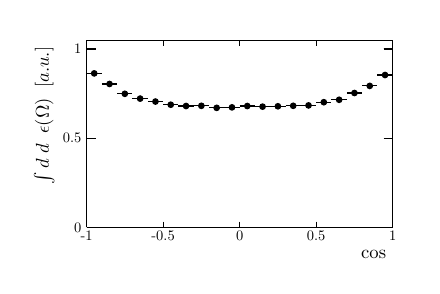
\begin{tikzpicture}
\pgfdeclareplotmark{cross} {
\pgfpathmoveto{\pgfpoint{-0.3\pgfplotmarksize}{\pgfplotmarksize}}
\pgfpathlineto{\pgfpoint{+0.3\pgfplotmarksize}{\pgfplotmarksize}}
\pgfpathlineto{\pgfpoint{+0.3\pgfplotmarksize}{0.3\pgfplotmarksize}}
\pgfpathlineto{\pgfpoint{+1\pgfplotmarksize}{0.3\pgfplotmarksize}}
\pgfpathlineto{\pgfpoint{+1\pgfplotmarksize}{-0.3\pgfplotmarksize}}
\pgfpathlineto{\pgfpoint{+0.3\pgfplotmarksize}{-0.3\pgfplotmarksize}}
\pgfpathlineto{\pgfpoint{+0.3\pgfplotmarksize}{-1.\pgfplotmarksize}}
\pgfpathlineto{\pgfpoint{-0.3\pgfplotmarksize}{-1.\pgfplotmarksize}}
\pgfpathlineto{\pgfpoint{-0.3\pgfplotmarksize}{-0.3\pgfplotmarksize}}
\pgfpathlineto{\pgfpoint{-1.\pgfplotmarksize}{-0.3\pgfplotmarksize}}
\pgfpathlineto{\pgfpoint{-1.\pgfplotmarksize}{0.3\pgfplotmarksize}}
\pgfpathlineto{\pgfpoint{-0.3\pgfplotmarksize}{0.3\pgfplotmarksize}}
\pgfpathclose
\pgfusepathqstroke
}
\pgfdeclareplotmark{cross*} {
\pgfpathmoveto{\pgfpoint{-0.3\pgfplotmarksize}{\pgfplotmarksize}}
\pgfpathlineto{\pgfpoint{+0.3\pgfplotmarksize}{\pgfplotmarksize}}
\pgfpathlineto{\pgfpoint{+0.3\pgfplotmarksize}{0.3\pgfplotmarksize}}
\pgfpathlineto{\pgfpoint{+1\pgfplotmarksize}{0.3\pgfplotmarksize}}
\pgfpathlineto{\pgfpoint{+1\pgfplotmarksize}{-0.3\pgfplotmarksize}}
\pgfpathlineto{\pgfpoint{+0.3\pgfplotmarksize}{-0.3\pgfplotmarksize}}
\pgfpathlineto{\pgfpoint{+0.3\pgfplotmarksize}{-1.\pgfplotmarksize}}
\pgfpathlineto{\pgfpoint{-0.3\pgfplotmarksize}{-1.\pgfplotmarksize}}
\pgfpathlineto{\pgfpoint{-0.3\pgfplotmarksize}{-0.3\pgfplotmarksize}}
\pgfpathlineto{\pgfpoint{-1.\pgfplotmarksize}{-0.3\pgfplotmarksize}}
\pgfpathlineto{\pgfpoint{-1.\pgfplotmarksize}{0.3\pgfplotmarksize}}
\pgfpathlineto{\pgfpoint{-0.3\pgfplotmarksize}{0.3\pgfplotmarksize}}
\pgfpathclose
\pgfusepathqfillstroke
}
\pgfdeclareplotmark{newstar} {
\pgfpathmoveto{\pgfqpoint{0pt}{\pgfplotmarksize}}
\pgfpathlineto{\pgfqpointpolar{44}{0.5\pgfplotmarksize}}
\pgfpathlineto{\pgfqpointpolar{18}{\pgfplotmarksize}}
\pgfpathlineto{\pgfqpointpolar{-20}{0.5\pgfplotmarksize}}
\pgfpathlineto{\pgfqpointpolar{-54}{\pgfplotmarksize}}
\pgfpathlineto{\pgfqpointpolar{-90}{0.5\pgfplotmarksize}}
\pgfpathlineto{\pgfqpointpolar{234}{\pgfplotmarksize}}
\pgfpathlineto{\pgfqpointpolar{198}{0.5\pgfplotmarksize}}
\pgfpathlineto{\pgfqpointpolar{162}{\pgfplotmarksize}}
\pgfpathlineto{\pgfqpointpolar{134}{0.5\pgfplotmarksize}}
\pgfpathclose
\pgfusepathqstroke
}
\pgfdeclareplotmark{newstar*} {
\pgfpathmoveto{\pgfqpoint{0pt}{\pgfplotmarksize}}
\pgfpathlineto{\pgfqpointpolar{44}{0.5\pgfplotmarksize}}
\pgfpathlineto{\pgfqpointpolar{18}{\pgfplotmarksize}}
\pgfpathlineto{\pgfqpointpolar{-20}{0.5\pgfplotmarksize}}
\pgfpathlineto{\pgfqpointpolar{-54}{\pgfplotmarksize}}
\pgfpathlineto{\pgfqpointpolar{-90}{0.5\pgfplotmarksize}}
\pgfpathlineto{\pgfqpointpolar{234}{\pgfplotmarksize}}
\pgfpathlineto{\pgfqpointpolar{198}{0.5\pgfplotmarksize}}
\pgfpathlineto{\pgfqpointpolar{162}{\pgfplotmarksize}}
\pgfpathlineto{\pgfqpointpolar{134}{0.5\pgfplotmarksize}}
\pgfpathclose
\pgfusepathqfillstroke
}
\definecolor{c}{rgb}{1,1,1};
\draw [color=c, fill=c] (5.1,3.20034) rectangle (9.9,6.21242);
\draw [color=c, fill=c] (5.772,3.68227) rectangle (9.66,6.06181);
\definecolor{c}{rgb}{0,0,0};
\draw [c] (5.772,3.68227) -- (5.772,6.06181) -- (9.66,6.06181) -- (9.66,3.68227) -- (5.772,3.68227);
\draw [c,line width=0.4] (5.8692,5.62691) -- (5.8692,5.63874);
\draw [c,line width=0.4] (5.8692,5.63874) -- (5.8692,5.65057);
\draw [c,line width=0.4] (5.772,5.63874) -- (5.8692,5.63874);
\draw [c,line width=0.4] (5.8692,5.63874) -- (5.9664,5.63874);
\foreach \P in {(5.8692,5.63874)}{\draw[mark options={color=c,fill=c},mark size=2.402402pt,mark=*,mark size=1pt] plot coordinates {\P};}
\draw [c,line width=0.4] (6.0636,5.49391) -- (6.0636,5.50447);
\draw [c,line width=0.4] (6.0636,5.50447) -- (6.0636,5.51502);
\draw [c,line width=0.4] (5.9664,5.50447) -- (6.0636,5.50447);
\draw [c,line width=0.4] (6.0636,5.50447) -- (6.1608,5.50447);
\foreach \P in {(6.0636,5.50447)}{\draw[mark options={color=c,fill=c},mark size=2.402402pt,mark=*,mark size=1pt] plot coordinates {\P};}
\draw [c,line width=0.4] (6.258,5.36949) -- (6.258,5.37943);
\draw [c,line width=0.4] (6.258,5.37943) -- (6.258,5.38937);
\draw [c,line width=0.4] (6.1608,5.37943) -- (6.258,5.37943);
\draw [c,line width=0.4] (6.258,5.37943) -- (6.3552,5.37943);
\foreach \P in {(6.258,5.37943)}{\draw[mark options={color=c,fill=c},mark size=2.402402pt,mark=*,mark size=1pt] plot coordinates {\P};}
\draw [c,line width=0.4] (6.4524,5.30891) -- (6.4524,5.31858);
\draw [c,line width=0.4] (6.4524,5.31858) -- (6.4524,5.32825);
\draw [c,line width=0.4] (6.3552,5.31858) -- (6.4524,5.31858);
\draw [c,line width=0.4] (6.4524,5.31858) -- (6.5496,5.31858);
\foreach \P in {(6.4524,5.31858)}{\draw[mark options={color=c,fill=c},mark size=2.402402pt,mark=*,mark size=1pt] plot coordinates {\P};}
\draw [c,line width=0.4] (6.6468,5.27176) -- (6.6468,5.2813);
\draw [c,line width=0.4] (6.6468,5.2813) -- (6.6468,5.29083);
\draw [c,line width=0.4] (6.5496,5.2813) -- (6.6468,5.2813);
\draw [c,line width=0.4] (6.6468,5.2813) -- (6.744,5.2813);
\foreach \P in {(6.6468,5.2813)}{\draw[mark options={color=c,fill=c},mark size=2.402402pt,mark=*,mark size=1pt] plot coordinates {\P};}
\draw [c,line width=0.4] (6.8412,5.23139) -- (6.8412,5.24083);
\draw [c,line width=0.4] (6.8412,5.24083) -- (6.8412,5.25027);
\draw [c,line width=0.4] (6.744,5.24083) -- (6.8412,5.24083);
\draw [c,line width=0.4] (6.8412,5.24083) -- (6.9384,5.24083);
\foreach \P in {(6.8412,5.24083)}{\draw[mark options={color=c,fill=c},mark size=2.402402pt,mark=*,mark size=1pt] plot coordinates {\P};}
\draw [c,line width=0.4] (7.0356,5.21504) -- (7.0356,5.22447);
\draw [c,line width=0.4] (7.0356,5.22447) -- (7.0356,5.2339);
\draw [c,line width=0.4] (6.9384,5.22447) -- (7.0356,5.22447);
\draw [c,line width=0.4] (7.0356,5.22447) -- (7.1328,5.22447);
\foreach \P in {(7.0356,5.22447)}{\draw[mark options={color=c,fill=c},mark size=2.402402pt,mark=*,mark size=1pt] plot coordinates {\P};}
\draw [c,line width=0.4] (7.23,5.21749) -- (7.23,5.22703);
\draw [c,line width=0.4] (7.23,5.22703) -- (7.23,5.23658);
\draw [c,line width=0.4] (7.1328,5.22703) -- (7.23,5.22703);
\draw [c,line width=0.4] (7.23,5.22703) -- (7.3272,5.22703);
\foreach \P in {(7.23,5.22703)}{\draw[mark options={color=c,fill=c},mark size=2.402402pt,mark=*,mark size=1pt] plot coordinates {\P};}
\draw [c,line width=0.4] (7.4244,5.19173) -- (7.4244,5.20122);
\draw [c,line width=0.4] (7.4244,5.20122) -- (7.4244,5.21071);
\draw [c,line width=0.4] (7.3272,5.20122) -- (7.4244,5.20122);
\draw [c,line width=0.4] (7.4244,5.20122) -- (7.5216,5.20122);
\foreach \P in {(7.4244,5.20122)}{\draw[mark options={color=c,fill=c},mark size=2.402402pt,mark=*,mark size=1pt] plot coordinates {\P};}
\draw [c,line width=0.4] (7.6188,5.19782) -- (7.6188,5.20735);
\draw [c,line width=0.4] (7.6188,5.20735) -- (7.6188,5.21689);
\draw [c,line width=0.4] (7.5216,5.20735) -- (7.6188,5.20735);
\draw [c,line width=0.4] (7.6188,5.20735) -- (7.716,5.20735);
\foreach \P in {(7.6188,5.20735)}{\draw[mark options={color=c,fill=c},mark size=2.402402pt,mark=*,mark size=1pt] plot coordinates {\P};}
\draw [c,line width=0.4] (7.8132,5.21472) -- (7.8132,5.22439);
\draw [c,line width=0.4] (7.8132,5.22439) -- (7.8132,5.23406);
\draw [c,line width=0.4] (7.716,5.22439) -- (7.8132,5.22439);
\draw [c,line width=0.4] (7.8132,5.22439) -- (7.9104,5.22439);
\foreach \P in {(7.8132,5.22439)}{\draw[mark options={color=c,fill=c},mark size=2.402402pt,mark=*,mark size=1pt] plot coordinates {\P};}
\draw [c,line width=0.4] (8.0076,5.20692) -- (8.0076,5.21648);
\draw [c,line width=0.4] (8.0076,5.21648) -- (8.0076,5.22604);
\draw [c,line width=0.4] (7.9104,5.21648) -- (8.0076,5.21648);
\draw [c,line width=0.4] (8.0076,5.21648) -- (8.1048,5.21648);
\foreach \P in {(8.0076,5.21648)}{\draw[mark options={color=c,fill=c},mark size=2.402402pt,mark=*,mark size=1pt] plot coordinates {\P};}
\draw [c,line width=0.4] (8.202,5.21158) -- (8.202,5.22108);
\draw [c,line width=0.4] (8.202,5.22108) -- (8.202,5.23059);
\draw [c,line width=0.4] (8.1048,5.22108) -- (8.202,5.22108);
\draw [c,line width=0.4] (8.202,5.22108) -- (8.2992,5.22108);
\foreach \P in {(8.202,5.22108)}{\draw[mark options={color=c,fill=c},mark size=2.402402pt,mark=*,mark size=1pt] plot coordinates {\P};}
\draw [c,line width=0.4] (8.3964,5.21763) -- (8.3964,5.22708);
\draw [c,line width=0.4] (8.3964,5.22708) -- (8.3964,5.23653);
\draw [c,line width=0.4] (8.2992,5.22708) -- (8.3964,5.22708);
\draw [c,line width=0.4] (8.3964,5.22708) -- (8.4936,5.22708);
\foreach \P in {(8.3964,5.22708)}{\draw[mark options={color=c,fill=c},mark size=2.402402pt,mark=*,mark size=1pt] plot coordinates {\P};}
\draw [c,line width=0.4] (8.5908,5.22277) -- (8.5908,5.2322);
\draw [c,line width=0.4] (8.5908,5.2322) -- (8.5908,5.24164);
\draw [c,line width=0.4] (8.4936,5.2322) -- (8.5908,5.2322);
\draw [c,line width=0.4] (8.5908,5.2322) -- (8.688,5.2322);
\foreach \P in {(8.5908,5.2322)}{\draw[mark options={color=c,fill=c},mark size=2.402402pt,mark=*,mark size=1pt] plot coordinates {\P};}
\draw [c,line width=0.4] (8.7852,5.26319) -- (8.7852,5.27274);
\draw [c,line width=0.4] (8.7852,5.27274) -- (8.7852,5.28229);
\draw [c,line width=0.4] (8.688,5.27274) -- (8.7852,5.27274);
\draw [c,line width=0.4] (8.7852,5.27274) -- (8.8824,5.27274);
\foreach \P in {(8.7852,5.27274)}{\draw[mark options={color=c,fill=c},mark size=2.402402pt,mark=*,mark size=1pt] plot coordinates {\P};}
\draw [c,line width=0.4] (8.9796,5.29385) -- (8.9796,5.30347);
\draw [c,line width=0.4] (8.9796,5.30347) -- (8.9796,5.31309);
\draw [c,line width=0.4] (8.8824,5.30347) -- (8.9796,5.30347);
\draw [c,line width=0.4] (8.9796,5.30347) -- (9.0768,5.30347);
\foreach \P in {(8.9796,5.30347)}{\draw[mark options={color=c,fill=c},mark size=2.402402pt,mark=*,mark size=1pt] plot coordinates {\P};}
\draw [c,line width=0.4] (9.174,5.37964) -- (9.174,5.3896);
\draw [c,line width=0.4] (9.174,5.3896) -- (9.174,5.39955);
\draw [c,line width=0.4] (9.0768,5.3896) -- (9.174,5.3896);
\draw [c,line width=0.4] (9.174,5.3896) -- (9.2712,5.3896);
\foreach \P in {(9.174,5.3896)}{\draw[mark options={color=c,fill=c},mark size=2.402402pt,mark=*,mark size=1pt] plot coordinates {\P};}
\draw [c,line width=0.4] (9.3684,5.46945) -- (9.3684,5.47997);
\draw [c,line width=0.4] (9.3684,5.47997) -- (9.3684,5.49049);
\draw [c,line width=0.4] (9.2712,5.47997) -- (9.3684,5.47997);
\draw [c,line width=0.4] (9.3684,5.47997) -- (9.4656,5.47997);
\foreach \P in {(9.3684,5.47997)}{\draw[mark options={color=c,fill=c},mark size=2.402402pt,mark=*,mark size=1pt] plot coordinates {\P};}
\draw [c,line width=0.4] (9.5628,5.60608) -- (9.5628,5.61823);
\draw [c,line width=0.4] (9.5628,5.61823) -- (9.5628,5.63039);
\draw [c,line width=0.4] (9.4656,5.61823) -- (9.5628,5.61823);
\draw [c,line width=0.4] (9.5628,5.61823) -- (9.66,5.61823);
\foreach \P in {(9.5628,5.61823)}{\draw[mark options={color=c,fill=c},mark size=2.402402pt,mark=*,mark size=1pt] plot coordinates {\P};}
\draw [c,line width=0.4] (5.772,3.68227) -- (9.66,3.68227);
\draw [anchor= east] (9.66,3.34492) node[scale=0.672711, rotate=0]{$\cos\thetamu$};
\draw [c,line width=0.4] (5.772,3.75546) -- (5.772,3.68227);
\draw [c,line width=0.4] (6.744,3.75546) -- (6.744,3.68227);
\draw [c,line width=0.4] (7.716,3.75546) -- (7.716,3.68227);
\draw [c,line width=0.4] (8.688,3.75546) -- (8.688,3.68227);
\draw [c,line width=0.4] (9.66,3.75546) -- (9.66,3.68227);
\draw [anchor=base] (5.772,3.51962) node[scale=0.52322, rotate=0]{-1};
\draw [anchor=base] (6.744,3.51962) node[scale=0.52322, rotate=0]{-0.5};
\draw [anchor=base] (7.716,3.51962) node[scale=0.52322, rotate=0]{0};
\draw [anchor=base] (8.688,3.51962) node[scale=0.52322, rotate=0]{0.5};
\draw [anchor=base] (9.66,3.51962) node[scale=0.52322, rotate=0]{1};
\draw [c,line width=0.4] (5.772,6.06181) -- (9.66,6.06181);
\draw [c,line width=0.4] (5.772,5.98862) -- (5.772,6.06181);
\draw [c,line width=0.4] (6.744,5.98862) -- (6.744,6.06181);
\draw [c,line width=0.4] (7.716,5.98862) -- (7.716,6.06181);
\draw [c,line width=0.4] (8.688,5.98862) -- (8.688,6.06181);
\draw [c,line width=0.4] (9.66,5.98862) -- (9.66,6.06181);
\draw [c,line width=0.4] (5.772,3.68227) -- (5.772,6.06181);
\draw [anchor= east] (5.2344,6.06181) node[scale=0.672711, rotate=90]{$\int d\thetaK \; d\phihel \;\; \epsilon(\Omega) \;\; [\text{a.u.}]$};
\draw [c,line width=0.4] (5.88576,3.68227) -- (5.772,3.68227);
\draw [c,line width=0.4] (5.88576,4.81538) -- (5.772,4.81538);
\draw [c,line width=0.4] (5.88576,5.9485) -- (5.772,5.9485);
\draw [c,line width=0.4] (5.88576,5.9485) -- (5.772,5.9485);
\draw [anchor= east] (5.772,3.68227) node[scale=0.52322, rotate=0]{0};
\draw [anchor= east] (5.772,4.81538) node[scale=0.52322, rotate=0]{0.5};
\draw [anchor= east] (5.772,5.9485) node[scale=0.52322, rotate=0]{1};
\draw [c,line width=0.4] (9.66,3.68227) -- (9.66,6.06181);
\draw [c,line width=0.4] (9.54624,3.68227) -- (9.66,3.68227);
\draw [c,line width=0.4] (9.54624,4.81538) -- (9.66,4.81538);
\draw [c,line width=0.4] (9.54624,5.9485) -- (9.66,5.9485);
\draw [c,line width=0.4] (9.54624,5.9485) -- (9.66,5.9485);
\end{tikzpicture}
}
    \caption{}
    \label{angAcc_ctl}
  \end{subfigure}
  \vspace*{0.02\textwidth}
  \begin{subfigure}{0.49\textwidth}
    \raggedright
    \tikzsetnextfilename{eff_mc_helphi_allKaons_binall}
    \scalebox{1.12}{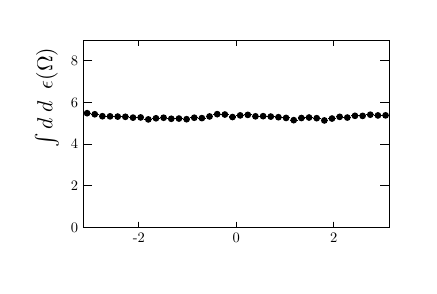
\begin{tikzpicture}
\pgfdeclareplotmark{cross} {
\pgfpathmoveto{\pgfpoint{-0.3\pgfplotmarksize}{\pgfplotmarksize}}
\pgfpathlineto{\pgfpoint{+0.3\pgfplotmarksize}{\pgfplotmarksize}}
\pgfpathlineto{\pgfpoint{+0.3\pgfplotmarksize}{0.3\pgfplotmarksize}}
\pgfpathlineto{\pgfpoint{+1\pgfplotmarksize}{0.3\pgfplotmarksize}}
\pgfpathlineto{\pgfpoint{+1\pgfplotmarksize}{-0.3\pgfplotmarksize}}
\pgfpathlineto{\pgfpoint{+0.3\pgfplotmarksize}{-0.3\pgfplotmarksize}}
\pgfpathlineto{\pgfpoint{+0.3\pgfplotmarksize}{-1.\pgfplotmarksize}}
\pgfpathlineto{\pgfpoint{-0.3\pgfplotmarksize}{-1.\pgfplotmarksize}}
\pgfpathlineto{\pgfpoint{-0.3\pgfplotmarksize}{-0.3\pgfplotmarksize}}
\pgfpathlineto{\pgfpoint{-1.\pgfplotmarksize}{-0.3\pgfplotmarksize}}
\pgfpathlineto{\pgfpoint{-1.\pgfplotmarksize}{0.3\pgfplotmarksize}}
\pgfpathlineto{\pgfpoint{-0.3\pgfplotmarksize}{0.3\pgfplotmarksize}}
\pgfpathclose
\pgfusepathqstroke
}
\pgfdeclareplotmark{cross*} {
\pgfpathmoveto{\pgfpoint{-0.3\pgfplotmarksize}{\pgfplotmarksize}}
\pgfpathlineto{\pgfpoint{+0.3\pgfplotmarksize}{\pgfplotmarksize}}
\pgfpathlineto{\pgfpoint{+0.3\pgfplotmarksize}{0.3\pgfplotmarksize}}
\pgfpathlineto{\pgfpoint{+1\pgfplotmarksize}{0.3\pgfplotmarksize}}
\pgfpathlineto{\pgfpoint{+1\pgfplotmarksize}{-0.3\pgfplotmarksize}}
\pgfpathlineto{\pgfpoint{+0.3\pgfplotmarksize}{-0.3\pgfplotmarksize}}
\pgfpathlineto{\pgfpoint{+0.3\pgfplotmarksize}{-1.\pgfplotmarksize}}
\pgfpathlineto{\pgfpoint{-0.3\pgfplotmarksize}{-1.\pgfplotmarksize}}
\pgfpathlineto{\pgfpoint{-0.3\pgfplotmarksize}{-0.3\pgfplotmarksize}}
\pgfpathlineto{\pgfpoint{-1.\pgfplotmarksize}{-0.3\pgfplotmarksize}}
\pgfpathlineto{\pgfpoint{-1.\pgfplotmarksize}{0.3\pgfplotmarksize}}
\pgfpathlineto{\pgfpoint{-0.3\pgfplotmarksize}{0.3\pgfplotmarksize}}
\pgfpathclose
\pgfusepathqfillstroke
}
\pgfdeclareplotmark{newstar} {
\pgfpathmoveto{\pgfqpoint{0pt}{\pgfplotmarksize}}
\pgfpathlineto{\pgfqpointpolar{44}{0.5\pgfplotmarksize}}
\pgfpathlineto{\pgfqpointpolar{18}{\pgfplotmarksize}}
\pgfpathlineto{\pgfqpointpolar{-20}{0.5\pgfplotmarksize}}
\pgfpathlineto{\pgfqpointpolar{-54}{\pgfplotmarksize}}
\pgfpathlineto{\pgfqpointpolar{-90}{0.5\pgfplotmarksize}}
\pgfpathlineto{\pgfqpointpolar{234}{\pgfplotmarksize}}
\pgfpathlineto{\pgfqpointpolar{198}{0.5\pgfplotmarksize}}
\pgfpathlineto{\pgfqpointpolar{162}{\pgfplotmarksize}}
\pgfpathlineto{\pgfqpointpolar{134}{0.5\pgfplotmarksize}}
\pgfpathclose
\pgfusepathqstroke
}
\pgfdeclareplotmark{newstar*} {
\pgfpathmoveto{\pgfqpoint{0pt}{\pgfplotmarksize}}
\pgfpathlineto{\pgfqpointpolar{44}{0.5\pgfplotmarksize}}
\pgfpathlineto{\pgfqpointpolar{18}{\pgfplotmarksize}}
\pgfpathlineto{\pgfqpointpolar{-20}{0.5\pgfplotmarksize}}
\pgfpathlineto{\pgfqpointpolar{-54}{\pgfplotmarksize}}
\pgfpathlineto{\pgfqpointpolar{-90}{0.5\pgfplotmarksize}}
\pgfpathlineto{\pgfqpointpolar{234}{\pgfplotmarksize}}
\pgfpathlineto{\pgfqpointpolar{198}{0.5\pgfplotmarksize}}
\pgfpathlineto{\pgfqpointpolar{162}{\pgfplotmarksize}}
\pgfpathlineto{\pgfqpointpolar{134}{0.5\pgfplotmarksize}}
\pgfpathclose
\pgfusepathqfillstroke
}
\definecolor{c}{rgb}{1,1,1};
\draw [color=c, fill=c] (0.1,0.0627517) rectangle (4.9,3.07483);
\draw [color=c, fill=c] (0.772,0.544685) rectangle (4.66,2.92423);
\definecolor{c}{rgb}{0,0,0};
\draw [c] (0.772,0.544685) -- (0.772,2.92423) -- (4.66,2.92423) -- (4.66,0.544685) -- (0.772,0.544685);
\draw [c,line width=0.4] (0.8206,1.98653) -- (0.8206,1.99592);
\draw [c,line width=0.4] (0.8206,1.99592) -- (0.8206,2.00531);
\draw [c,line width=0.4] (0.772,1.99592) -- (0.8206,1.99592);
\draw [c,line width=0.4] (0.8206,1.99592) -- (0.8692,1.99592);
\foreach \P in {(0.8206,1.99592)}{\draw[mark options={color=c,fill=c},mark size=2.402402pt,mark=*,mark size=1pt] plot coordinates {\P};}
\draw [c,line width=0.4] (0.9178,1.97266) -- (0.9178,1.982);
\draw [c,line width=0.4] (0.9178,1.982) -- (0.9178,1.99135);
\draw [c,line width=0.4] (0.8692,1.982) -- (0.9178,1.982);
\draw [c,line width=0.4] (0.9178,1.982) -- (0.9664,1.982);
\foreach \P in {(0.9178,1.982)}{\draw[mark options={color=c,fill=c},mark size=2.402402pt,mark=*,mark size=1pt] plot coordinates {\P};}
\draw [c,line width=0.4] (1.015,1.94805) -- (1.015,1.95731);
\draw [c,line width=0.4] (1.015,1.95731) -- (1.015,1.96658);
\draw [c,line width=0.4] (0.9664,1.95731) -- (1.015,1.95731);
\draw [c,line width=0.4] (1.015,1.95731) -- (1.0636,1.95731);
\foreach \P in {(1.015,1.95731)}{\draw[mark options={color=c,fill=c},mark size=2.402402pt,mark=*,mark size=1pt] plot coordinates {\P};}
\draw [c,line width=0.4] (1.1122,1.94635) -- (1.1122,1.9556);
\draw [c,line width=0.4] (1.1122,1.9556) -- (1.1122,1.96486);
\draw [c,line width=0.4] (1.0636,1.9556) -- (1.1122,1.9556);
\draw [c,line width=0.4] (1.1122,1.9556) -- (1.1608,1.9556);
\foreach \P in {(1.1122,1.9556)}{\draw[mark options={color=c,fill=c},mark size=2.402402pt,mark=*,mark size=1pt] plot coordinates {\P};}
\draw [c,line width=0.4] (1.2094,1.94343) -- (1.2094,1.95268);
\draw [c,line width=0.4] (1.2094,1.95268) -- (1.2094,1.96192);
\draw [c,line width=0.4] (1.1608,1.95268) -- (1.2094,1.95268);
\draw [c,line width=0.4] (1.2094,1.95268) -- (1.258,1.95268);
\foreach \P in {(1.2094,1.95268)}{\draw[mark options={color=c,fill=c},mark size=2.402402pt,mark=*,mark size=1pt] plot coordinates {\P};}
\draw [c,line width=0.4] (1.3066,1.94072) -- (1.3066,1.94996);
\draw [c,line width=0.4] (1.3066,1.94996) -- (1.3066,1.9592);
\draw [c,line width=0.4] (1.258,1.94996) -- (1.3066,1.94996);
\draw [c,line width=0.4] (1.3066,1.94996) -- (1.3552,1.94996);
\foreach \P in {(1.3066,1.94996)}{\draw[mark options={color=c,fill=c},mark size=2.402402pt,mark=*,mark size=1pt] plot coordinates {\P};}
\draw [c,line width=0.4] (1.4038,1.93026) -- (1.4038,1.93947);
\draw [c,line width=0.4] (1.4038,1.93947) -- (1.4038,1.94867);
\draw [c,line width=0.4] (1.3552,1.93947) -- (1.4038,1.93947);
\draw [c,line width=0.4] (1.4038,1.93947) -- (1.4524,1.93947);
\foreach \P in {(1.4038,1.93947)}{\draw[mark options={color=c,fill=c},mark size=2.402402pt,mark=*,mark size=1pt] plot coordinates {\P};}
\draw [c,line width=0.4] (1.501,1.93278) -- (1.501,1.94199);
\draw [c,line width=0.4] (1.501,1.94199) -- (1.501,1.9512);
\draw [c,line width=0.4] (1.4524,1.94199) -- (1.501,1.94199);
\draw [c,line width=0.4] (1.501,1.94199) -- (1.5496,1.94199);
\foreach \P in {(1.501,1.94199)}{\draw[mark options={color=c,fill=c},mark size=2.402402pt,mark=*,mark size=1pt] plot coordinates {\P};}
\draw [c,line width=0.4] (1.5982,1.9078) -- (1.5982,1.91693);
\draw [c,line width=0.4] (1.5982,1.91693) -- (1.5982,1.92606);
\draw [c,line width=0.4] (1.5496,1.91693) -- (1.5982,1.91693);
\draw [c,line width=0.4] (1.5982,1.91693) -- (1.6468,1.91693);
\foreach \P in {(1.5982,1.91693)}{\draw[mark options={color=c,fill=c},mark size=2.402402pt,mark=*,mark size=1pt] plot coordinates {\P};}
\draw [c,line width=0.4] (1.6954,1.922) -- (1.6954,1.93118);
\draw [c,line width=0.4] (1.6954,1.93118) -- (1.6954,1.94036);
\draw [c,line width=0.4] (1.6468,1.93118) -- (1.6954,1.93118);
\draw [c,line width=0.4] (1.6954,1.93118) -- (1.744,1.93118);
\foreach \P in {(1.6954,1.93118)}{\draw[mark options={color=c,fill=c},mark size=2.402402pt,mark=*,mark size=1pt] plot coordinates {\P};}
\draw [c,line width=0.4] (1.7926,1.92905) -- (1.7926,1.93825);
\draw [c,line width=0.4] (1.7926,1.93825) -- (1.7926,1.94746);
\draw [c,line width=0.4] (1.744,1.93825) -- (1.7926,1.93825);
\draw [c,line width=0.4] (1.7926,1.93825) -- (1.8412,1.93825);
\foreach \P in {(1.7926,1.93825)}{\draw[mark options={color=c,fill=c},mark size=2.402402pt,mark=*,mark size=1pt] plot coordinates {\P};}
\draw [c,line width=0.4] (1.8898,1.91573) -- (1.8898,1.92489);
\draw [c,line width=0.4] (1.8898,1.92489) -- (1.8898,1.93405);
\draw [c,line width=0.4] (1.8412,1.92489) -- (1.8898,1.92489);
\draw [c,line width=0.4] (1.8898,1.92489) -- (1.9384,1.92489);
\foreach \P in {(1.8898,1.92489)}{\draw[mark options={color=c,fill=c},mark size=2.402402pt,mark=*,mark size=1pt] plot coordinates {\P};}
\draw [c,line width=0.4] (1.987,1.91853) -- (1.987,1.9277);
\draw [c,line width=0.4] (1.987,1.9277) -- (1.987,1.93687);
\draw [c,line width=0.4] (1.9384,1.9277) -- (1.987,1.9277);
\draw [c,line width=0.4] (1.987,1.9277) -- (2.0356,1.9277);
\foreach \P in {(1.987,1.9277)}{\draw[mark options={color=c,fill=c},mark size=2.402402pt,mark=*,mark size=1pt] plot coordinates {\P};}
\draw [c,line width=0.4] (2.0842,1.91024) -- (2.0842,1.91938);
\draw [c,line width=0.4] (2.0842,1.91938) -- (2.0842,1.92852);
\draw [c,line width=0.4] (2.0356,1.91938) -- (2.0842,1.91938);
\draw [c,line width=0.4] (2.0842,1.91938) -- (2.1328,1.91938);
\foreach \P in {(2.0842,1.91938)}{\draw[mark options={color=c,fill=c},mark size=2.402402pt,mark=*,mark size=1pt] plot coordinates {\P};}
\draw [c,line width=0.4] (2.1814,1.92902) -- (2.1814,1.93822);
\draw [c,line width=0.4] (2.1814,1.93822) -- (2.1814,1.94742);
\draw [c,line width=0.4] (2.1328,1.93822) -- (2.1814,1.93822);
\draw [c,line width=0.4] (2.1814,1.93822) -- (2.23,1.93822);
\foreach \P in {(2.1814,1.93822)}{\draw[mark options={color=c,fill=c},mark size=2.402402pt,mark=*,mark size=1pt] plot coordinates {\P};}
\draw [c,line width=0.4] (2.2786,1.92407) -- (2.2786,1.93325);
\draw [c,line width=0.4] (2.2786,1.93325) -- (2.2786,1.94244);
\draw [c,line width=0.4] (2.23,1.93325) -- (2.2786,1.93325);
\draw [c,line width=0.4] (2.2786,1.93325) -- (2.3272,1.93325);
\foreach \P in {(2.2786,1.93325)}{\draw[mark options={color=c,fill=c},mark size=2.402402pt,mark=*,mark size=1pt] plot coordinates {\P};}
\draw [c,line width=0.4] (2.3758,1.94534) -- (2.3758,1.95459);
\draw [c,line width=0.4] (2.3758,1.95459) -- (2.3758,1.96385);
\draw [c,line width=0.4] (2.3272,1.95459) -- (2.3758,1.95459);
\draw [c,line width=0.4] (2.3758,1.95459) -- (2.4244,1.95459);
\foreach \P in {(2.3758,1.95459)}{\draw[mark options={color=c,fill=c},mark size=2.402402pt,mark=*,mark size=1pt] plot coordinates {\P};}
\draw [c,line width=0.4] (2.473,1.97421) -- (2.473,1.98356);
\draw [c,line width=0.4] (2.473,1.98356) -- (2.473,1.99291);
\draw [c,line width=0.4] (2.4244,1.98356) -- (2.473,1.98356);
\draw [c,line width=0.4] (2.473,1.98356) -- (2.5216,1.98356);
\foreach \P in {(2.473,1.98356)}{\draw[mark options={color=c,fill=c},mark size=2.402402pt,mark=*,mark size=1pt] plot coordinates {\P};}
\draw [c,line width=0.4] (2.5702,1.96938) -- (2.5702,1.97871);
\draw [c,line width=0.4] (2.5702,1.97871) -- (2.5702,1.98805);
\draw [c,line width=0.4] (2.5216,1.97871) -- (2.5702,1.97871);
\draw [c,line width=0.4] (2.5702,1.97871) -- (2.6188,1.97871);
\foreach \P in {(2.5702,1.97871)}{\draw[mark options={color=c,fill=c},mark size=2.402402pt,mark=*,mark size=1pt] plot coordinates {\P};}
\draw [c,line width=0.4] (2.6674,1.93764) -- (2.6674,1.94687);
\draw [c,line width=0.4] (2.6674,1.94687) -- (2.6674,1.9561);
\draw [c,line width=0.4] (2.6188,1.94687) -- (2.6674,1.94687);
\draw [c,line width=0.4] (2.6674,1.94687) -- (2.716,1.94687);
\foreach \P in {(2.6674,1.94687)}{\draw[mark options={color=c,fill=c},mark size=2.402402pt,mark=*,mark size=1pt] plot coordinates {\P};}
\draw [c,line width=0.4] (2.7646,1.9586) -- (2.7646,1.9679);
\draw [c,line width=0.4] (2.7646,1.9679) -- (2.7646,1.9772);
\draw [c,line width=0.4] (2.716,1.9679) -- (2.7646,1.9679);
\draw [c,line width=0.4] (2.7646,1.9679) -- (2.8132,1.9679);
\foreach \P in {(2.7646,1.9679)}{\draw[mark options={color=c,fill=c},mark size=2.402402pt,mark=*,mark size=1pt] plot coordinates {\P};}
\draw [c,line width=0.4] (2.8618,1.96503) -- (2.8618,1.97435);
\draw [c,line width=0.4] (2.8618,1.97435) -- (2.8618,1.98367);
\draw [c,line width=0.4] (2.8132,1.97435) -- (2.8618,1.97435);
\draw [c,line width=0.4] (2.8618,1.97435) -- (2.9104,1.97435);
\foreach \P in {(2.8618,1.97435)}{\draw[mark options={color=c,fill=c},mark size=2.402402pt,mark=*,mark size=1pt] plot coordinates {\P};}
\draw [c,line width=0.4] (2.959,1.94673) -- (2.959,1.95599);
\draw [c,line width=0.4] (2.959,1.95599) -- (2.959,1.96525);
\draw [c,line width=0.4] (2.9104,1.95599) -- (2.959,1.95599);
\draw [c,line width=0.4] (2.959,1.95599) -- (3.0076,1.95599);
\foreach \P in {(2.959,1.95599)}{\draw[mark options={color=c,fill=c},mark size=2.402402pt,mark=*,mark size=1pt] plot coordinates {\P};}
\draw [c,line width=0.4] (3.0562,1.9488) -- (3.0562,1.95807);
\draw [c,line width=0.4] (3.0562,1.95807) -- (3.0562,1.96733);
\draw [c,line width=0.4] (3.0076,1.95807) -- (3.0562,1.95807);
\draw [c,line width=0.4] (3.0562,1.95807) -- (3.1048,1.95807);
\foreach \P in {(3.0562,1.95807)}{\draw[mark options={color=c,fill=c},mark size=2.402402pt,mark=*,mark size=1pt] plot coordinates {\P};}
\draw [c,line width=0.4] (3.1534,1.94343) -- (3.1534,1.95268);
\draw [c,line width=0.4] (3.1534,1.95268) -- (3.1534,1.96193);
\draw [c,line width=0.4] (3.1048,1.95268) -- (3.1534,1.95268);
\draw [c,line width=0.4] (3.1534,1.95268) -- (3.202,1.95268);
\foreach \P in {(3.1534,1.95268)}{\draw[mark options={color=c,fill=c},mark size=2.402402pt,mark=*,mark size=1pt] plot coordinates {\P};}
\draw [c,line width=0.4] (3.2506,1.93572) -- (3.2506,1.94495);
\draw [c,line width=0.4] (3.2506,1.94495) -- (3.2506,1.95417);
\draw [c,line width=0.4] (3.202,1.94495) -- (3.2506,1.94495);
\draw [c,line width=0.4] (3.2506,1.94495) -- (3.2992,1.94495);
\foreach \P in {(3.2506,1.94495)}{\draw[mark options={color=c,fill=c},mark size=2.402402pt,mark=*,mark size=1pt] plot coordinates {\P};}
\draw [c,line width=0.4] (3.3478,1.92627) -- (3.3478,1.93546);
\draw [c,line width=0.4] (3.3478,1.93546) -- (3.3478,1.94465);
\draw [c,line width=0.4] (3.2992,1.93546) -- (3.3478,1.93546);
\draw [c,line width=0.4] (3.3478,1.93546) -- (3.3964,1.93546);
\foreach \P in {(3.3478,1.93546)}{\draw[mark options={color=c,fill=c},mark size=2.402402pt,mark=*,mark size=1pt] plot coordinates {\P};}
\draw [c,line width=0.4] (3.445,1.8983) -- (3.445,1.9074);
\draw [c,line width=0.4] (3.445,1.9074) -- (3.445,1.91649);
\draw [c,line width=0.4] (3.3964,1.9074) -- (3.445,1.9074);
\draw [c,line width=0.4] (3.445,1.9074) -- (3.4936,1.9074);
\foreach \P in {(3.445,1.9074)}{\draw[mark options={color=c,fill=c},mark size=2.402402pt,mark=*,mark size=1pt] plot coordinates {\P};}
\draw [c,line width=0.4] (3.5422,1.9253) -- (3.5422,1.93448);
\draw [c,line width=0.4] (3.5422,1.93448) -- (3.5422,1.94367);
\draw [c,line width=0.4] (3.4936,1.93448) -- (3.5422,1.93448);
\draw [c,line width=0.4] (3.5422,1.93448) -- (3.5908,1.93448);
\foreach \P in {(3.5422,1.93448)}{\draw[mark options={color=c,fill=c},mark size=2.402402pt,mark=*,mark size=1pt] plot coordinates {\P};}
\draw [c,line width=0.4] (3.6394,1.93164) -- (3.6394,1.94085);
\draw [c,line width=0.4] (3.6394,1.94085) -- (3.6394,1.95006);
\draw [c,line width=0.4] (3.5908,1.94085) -- (3.6394,1.94085);
\draw [c,line width=0.4] (3.6394,1.94085) -- (3.688,1.94085);
\foreach \P in {(3.6394,1.94085)}{\draw[mark options={color=c,fill=c},mark size=2.402402pt,mark=*,mark size=1pt] plot coordinates {\P};}
\draw [c,line width=0.4] (3.7366,1.92319) -- (3.7366,1.93238);
\draw [c,line width=0.4] (3.7366,1.93238) -- (3.7366,1.94156);
\draw [c,line width=0.4] (3.688,1.93238) -- (3.7366,1.93238);
\draw [c,line width=0.4] (3.7366,1.93238) -- (3.7852,1.93238);
\foreach \P in {(3.7366,1.93238)}{\draw[mark options={color=c,fill=c},mark size=2.402402pt,mark=*,mark size=1pt] plot coordinates {\P};}
\draw [c,line width=0.4] (3.8338,1.89466) -- (3.8338,1.90375);
\draw [c,line width=0.4] (3.8338,1.90375) -- (3.8338,1.91283);
\draw [c,line width=0.4] (3.7852,1.90375) -- (3.8338,1.90375);
\draw [c,line width=0.4] (3.8338,1.90375) -- (3.8824,1.90375);
\foreach \P in {(3.8338,1.90375)}{\draw[mark options={color=c,fill=c},mark size=2.402402pt,mark=*,mark size=1pt] plot coordinates {\P};}
\draw [c,line width=0.4] (3.931,1.91882) -- (3.931,1.92799);
\draw [c,line width=0.4] (3.931,1.92799) -- (3.931,1.93716);
\draw [c,line width=0.4] (3.8824,1.92799) -- (3.931,1.92799);
\draw [c,line width=0.4] (3.931,1.92799) -- (3.9796,1.92799);
\foreach \P in {(3.931,1.92799)}{\draw[mark options={color=c,fill=c},mark size=2.402402pt,mark=*,mark size=1pt] plot coordinates {\P};}
\draw [c,line width=0.4] (4.0282,1.94005) -- (4.0282,1.94929);
\draw [c,line width=0.4] (4.0282,1.94929) -- (4.0282,1.95853);
\draw [c,line width=0.4] (3.9796,1.94929) -- (4.0282,1.94929);
\draw [c,line width=0.4] (4.0282,1.94929) -- (4.0768,1.94929);
\foreach \P in {(4.0282,1.94929)}{\draw[mark options={color=c,fill=c},mark size=2.402402pt,mark=*,mark size=1pt] plot coordinates {\P};}
\draw [c,line width=0.4] (4.1254,1.93127) -- (4.1254,1.94048);
\draw [c,line width=0.4] (4.1254,1.94048) -- (4.1254,1.94969);
\draw [c,line width=0.4] (4.0768,1.94048) -- (4.1254,1.94048);
\draw [c,line width=0.4] (4.1254,1.94048) -- (4.174,1.94048);
\foreach \P in {(4.1254,1.94048)}{\draw[mark options={color=c,fill=c},mark size=2.402402pt,mark=*,mark size=1pt] plot coordinates {\P};}
\draw [c,line width=0.4] (4.2226,1.95317) -- (4.2226,1.96245);
\draw [c,line width=0.4] (4.2226,1.96245) -- (4.2226,1.97173);
\draw [c,line width=0.4] (4.174,1.96245) -- (4.2226,1.96245);
\draw [c,line width=0.4] (4.2226,1.96245) -- (4.2712,1.96245);
\foreach \P in {(4.2226,1.96245)}{\draw[mark options={color=c,fill=c},mark size=2.402402pt,mark=*,mark size=1pt] plot coordinates {\P};}
\draw [c,line width=0.4] (4.3198,1.95225) -- (4.3198,1.96153);
\draw [c,line width=0.4] (4.3198,1.96153) -- (4.3198,1.9708);
\draw [c,line width=0.4] (4.2712,1.96153) -- (4.3198,1.96153);
\draw [c,line width=0.4] (4.3198,1.96153) -- (4.3684,1.96153);
\foreach \P in {(4.3198,1.96153)}{\draw[mark options={color=c,fill=c},mark size=2.402402pt,mark=*,mark size=1pt] plot coordinates {\P};}
\draw [c,line width=0.4] (4.417,1.96738) -- (4.417,1.97671);
\draw [c,line width=0.4] (4.417,1.97671) -- (4.417,1.98603);
\draw [c,line width=0.4] (4.3684,1.97671) -- (4.417,1.97671);
\draw [c,line width=0.4] (4.417,1.97671) -- (4.4656,1.97671);
\foreach \P in {(4.417,1.97671)}{\draw[mark options={color=c,fill=c},mark size=2.402402pt,mark=*,mark size=1pt] plot coordinates {\P};}
\draw [c,line width=0.4] (4.5142,1.95805) -- (4.5142,1.96735);
\draw [c,line width=0.4] (4.5142,1.96735) -- (4.5142,1.97665);
\draw [c,line width=0.4] (4.4656,1.96735) -- (4.5142,1.96735);
\draw [c,line width=0.4] (4.5142,1.96735) -- (4.5628,1.96735);
\foreach \P in {(4.5142,1.96735)}{\draw[mark options={color=c,fill=c},mark size=2.402402pt,mark=*,mark size=1pt] plot coordinates {\P};}
\draw [c,line width=0.4] (4.6114,1.95904) -- (4.6114,1.96834);
\draw [c,line width=0.4] (4.6114,1.96834) -- (4.6114,1.97764);
\draw [c,line width=0.4] (4.5628,1.96834) -- (4.6114,1.96834);
\draw [c,line width=0.4] (4.6114,1.96834) -- (4.66,1.96834);
\foreach \P in {(4.6114,1.96834)}{\draw[mark options={color=c,fill=c},mark size=2.402402pt,mark=*,mark size=1pt] plot coordinates {\P};}
\draw [c,line width=0.4] (0.772,0.544685) -- (4.66,0.544685);
\draw [anchor= east] (4.66,0.255525) node[scale=0.78483, rotate=0]{$\phihel$};
\draw [c,line width=0.4] (1.47778,0.617878) -- (1.47778,0.544685);
\draw [c,line width=0.4] (2.716,0.617878) -- (2.716,0.544685);
\draw [c,line width=0.4] (3.95422,0.617878) -- (3.95422,0.544685);
\draw [c,line width=0.4] (1.47778,0.617878) -- (1.47778,0.544685);
\draw [c,line width=0.4] (3.95422,0.617878) -- (3.95422,0.544685);
\draw [anchor=base] (1.47778,0.351911) node[scale=0.52322, rotate=0]{-2};
\draw [anchor=base] (2.716,0.351911) node[scale=0.52322, rotate=0]{0};
\draw [anchor=base] (3.95422,0.351911) node[scale=0.52322, rotate=0]{2};
\draw [c,line width=0.4] (0.772,2.92423) -- (4.66,2.92423);
\draw [c,line width=0.4] (1.47778,2.85103) -- (1.47778,2.92423);
\draw [c,line width=0.4] (2.716,2.85103) -- (2.716,2.92423);
\draw [c,line width=0.4] (3.95422,2.85103) -- (3.95422,2.92423);
\draw [c,line width=0.4] (1.47778,2.85103) -- (1.47778,2.92423);
\draw [c,line width=0.4] (3.95422,2.85103) -- (3.95422,2.92423);
\draw [c,line width=0.4] (0.772,0.544685) -- (0.772,2.92423);
\draw [anchor= east] (0.3112,2.92423) node[scale=0.78483, rotate=90]{$\int d\thetaK \; d\thetamu \;\; \epsilon(\Omega) $};
\draw [c,line width=0.4] (0.88576,0.544685) -- (0.772,0.544685);
\draw [c,line width=0.4] (0.88576,1.07347) -- (0.772,1.07347);
\draw [c,line width=0.4] (0.88576,1.60226) -- (0.772,1.60226);
\draw [c,line width=0.4] (0.88576,2.13105) -- (0.772,2.13105);
\draw [c,line width=0.4] (0.88576,2.65983) -- (0.772,2.65983);
\draw [c,line width=0.4] (0.88576,2.65983) -- (0.772,2.65983);
\draw [anchor= east] (0.772,0.544685) node[scale=0.52322, rotate=0]{0};
\draw [anchor= east] (0.772,1.07347) node[scale=0.52322, rotate=0]{2};
\draw [anchor= east] (0.772,1.60226) node[scale=0.52322, rotate=0]{4};
\draw [anchor= east] (0.772,2.13105) node[scale=0.52322, rotate=0]{6};
\draw [anchor= east] (0.772,2.65983) node[scale=0.52322, rotate=0]{8};
\draw [c,line width=0.4] (4.66,0.544685) -- (4.66,2.92423);
\draw [c,line width=0.4] (4.54624,0.544685) -- (4.66,0.544685);
\draw [c,line width=0.4] (4.54624,1.07347) -- (4.66,1.07347);
\draw [c,line width=0.4] (4.54624,1.60226) -- (4.66,1.60226);
\draw [c,line width=0.4] (4.54624,2.13105) -- (4.66,2.13105);
\draw [c,line width=0.4] (4.54624,2.65983) -- (4.66,2.65983);
\draw [c,line width=0.4] (4.54624,2.65983) -- (4.66,2.65983);
\end{tikzpicture}
}
    \caption{}
    \label{angAcc_phi}
  \end{subfigure}
  \caption{Angular acceptance shape from simulated data. Each candidate has been assigned a weight. Each weight is
           equal to one over the integral of the \pdf that was used to generate the angular distribution of the simulated data.}
  \label{angAcc_all}
\end{figure}

The shape of the acceptance can be seen in \figref{angAcc_all}. The most striking feature is the drop of efficiency
close to $\cos\thetaK=1$. The later is mainly caused by one of the candidate selection requirements of \tabref{Bs2JpsiKstSelection},
specifically the requirement on the \kaon and \pion transverse momentum, \pt, to be larger that $500\mevc$.
Before attempting to explain the acceptance shape it is useful to illustrate how the decay angles are
distributed according to the \pdf of \equref{ang_terms}, \ie without any acceptance effect, see \figref{angDistr_all}.

Understanding the shape of the acceptance in the $\cos\thetaK$ projection begins with the observation
that the phase space region of $(\ptrans{\pi}-\cos\thetaK)$ is not uniformly populated. This is related to kinematic
constrains, explained in the next paragraph. Qualitatively speaking, it turns out that \Bs decays tend to cluster
close to the region of $(\ptrans{\pi}-\cos\thetaK|_{-1})$ compared to the $(\ptrans{\pi}-\cos\thetaK|_{+1})$ region.
This picture is less pronounced in the case of $(\ptrans{\kaon}-\cos\thetaK)$ phase space region, where the $\ptrans{\kaon}$
spectrum is harder and the $(\ptrans{\kaon}-\cos\thetaK)$ is more symmetric with respect to $\cos\thetaK$, see \figref{ctk_hadrons_pt}.
Given these correlations it follows that applying the \pt requirement on both \kaon and \pion makes the $\cos\thetaK$ distribution
asymmetric around $\cos\thetaK=0$.

\begin{figure}[t]
  \centering
  \begin{subfigure}{0.33\textwidth}
    \tikzsetnextfilename{mc_ang_ctk}
    \scalebox{0.65}{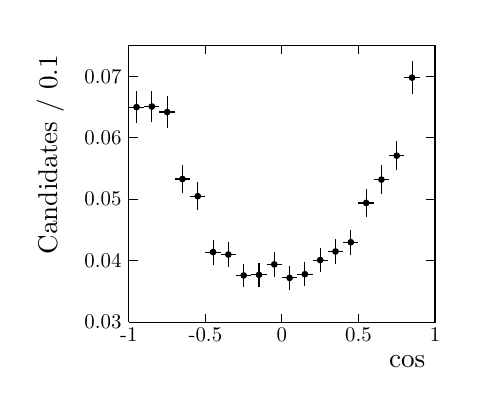
\begin{tikzpicture}
\pgfdeclareplotmark{cross} {
\pgfpathmoveto{\pgfpoint{-0.3\pgfplotmarksize}{\pgfplotmarksize}}
\pgfpathlineto{\pgfpoint{+0.3\pgfplotmarksize}{\pgfplotmarksize}}
\pgfpathlineto{\pgfpoint{+0.3\pgfplotmarksize}{0.3\pgfplotmarksize}}
\pgfpathlineto{\pgfpoint{+1\pgfplotmarksize}{0.3\pgfplotmarksize}}
\pgfpathlineto{\pgfpoint{+1\pgfplotmarksize}{-0.3\pgfplotmarksize}}
\pgfpathlineto{\pgfpoint{+0.3\pgfplotmarksize}{-0.3\pgfplotmarksize}}
\pgfpathlineto{\pgfpoint{+0.3\pgfplotmarksize}{-1.\pgfplotmarksize}}
\pgfpathlineto{\pgfpoint{-0.3\pgfplotmarksize}{-1.\pgfplotmarksize}}
\pgfpathlineto{\pgfpoint{-0.3\pgfplotmarksize}{-0.3\pgfplotmarksize}}
\pgfpathlineto{\pgfpoint{-1.\pgfplotmarksize}{-0.3\pgfplotmarksize}}
\pgfpathlineto{\pgfpoint{-1.\pgfplotmarksize}{0.3\pgfplotmarksize}}
\pgfpathlineto{\pgfpoint{-0.3\pgfplotmarksize}{0.3\pgfplotmarksize}}
\pgfpathclose
\pgfusepathqstroke
}
\pgfdeclareplotmark{cross*} {
\pgfpathmoveto{\pgfpoint{-0.3\pgfplotmarksize}{\pgfplotmarksize}}
\pgfpathlineto{\pgfpoint{+0.3\pgfplotmarksize}{\pgfplotmarksize}}
\pgfpathlineto{\pgfpoint{+0.3\pgfplotmarksize}{0.3\pgfplotmarksize}}
\pgfpathlineto{\pgfpoint{+1\pgfplotmarksize}{0.3\pgfplotmarksize}}
\pgfpathlineto{\pgfpoint{+1\pgfplotmarksize}{-0.3\pgfplotmarksize}}
\pgfpathlineto{\pgfpoint{+0.3\pgfplotmarksize}{-0.3\pgfplotmarksize}}
\pgfpathlineto{\pgfpoint{+0.3\pgfplotmarksize}{-1.\pgfplotmarksize}}
\pgfpathlineto{\pgfpoint{-0.3\pgfplotmarksize}{-1.\pgfplotmarksize}}
\pgfpathlineto{\pgfpoint{-0.3\pgfplotmarksize}{-0.3\pgfplotmarksize}}
\pgfpathlineto{\pgfpoint{-1.\pgfplotmarksize}{-0.3\pgfplotmarksize}}
\pgfpathlineto{\pgfpoint{-1.\pgfplotmarksize}{0.3\pgfplotmarksize}}
\pgfpathlineto{\pgfpoint{-0.3\pgfplotmarksize}{0.3\pgfplotmarksize}}
\pgfpathclose
\pgfusepathqfillstroke
}
\pgfdeclareplotmark{newstar} {
\pgfpathmoveto{\pgfqpoint{0pt}{\pgfplotmarksize}}
\pgfpathlineto{\pgfqpointpolar{44}{0.5\pgfplotmarksize}}
\pgfpathlineto{\pgfqpointpolar{18}{\pgfplotmarksize}}
\pgfpathlineto{\pgfqpointpolar{-20}{0.5\pgfplotmarksize}}
\pgfpathlineto{\pgfqpointpolar{-54}{\pgfplotmarksize}}
\pgfpathlineto{\pgfqpointpolar{-90}{0.5\pgfplotmarksize}}
\pgfpathlineto{\pgfqpointpolar{234}{\pgfplotmarksize}}
\pgfpathlineto{\pgfqpointpolar{198}{0.5\pgfplotmarksize}}
\pgfpathlineto{\pgfqpointpolar{162}{\pgfplotmarksize}}
\pgfpathlineto{\pgfqpointpolar{134}{0.5\pgfplotmarksize}}
\pgfpathclose
\pgfusepathqstroke
}
\pgfdeclareplotmark{newstar*} {
\pgfpathmoveto{\pgfqpoint{0pt}{\pgfplotmarksize}}
\pgfpathlineto{\pgfqpointpolar{44}{0.5\pgfplotmarksize}}
\pgfpathlineto{\pgfqpointpolar{18}{\pgfplotmarksize}}
\pgfpathlineto{\pgfqpointpolar{-20}{0.5\pgfplotmarksize}}
\pgfpathlineto{\pgfqpointpolar{-54}{\pgfplotmarksize}}
\pgfpathlineto{\pgfqpointpolar{-90}{0.5\pgfplotmarksize}}
\pgfpathlineto{\pgfqpointpolar{234}{\pgfplotmarksize}}
\pgfpathlineto{\pgfqpointpolar{198}{0.5\pgfplotmarksize}}
\pgfpathlineto{\pgfqpointpolar{162}{\pgfplotmarksize}}
\pgfpathlineto{\pgfqpointpolar{134}{0.5\pgfplotmarksize}}
\pgfpathclose
\pgfusepathqfillstroke
}
\definecolor{c}{rgb}{1,1,1};
\draw [color=c, fill=c] (0.1,0.0925676) rectangle (4.9,4.53581);
\draw [color=c, fill=c] (0.772,0.803486) rectangle (4.66,4.31365);
\definecolor{c}{rgb}{0,0,0};
\draw [c] (0.772,0.803486) -- (0.772,4.31365) -- (4.66,4.31365) -- (4.66,0.803486) -- (0.772,0.803486);
\draw [c,line width=0.4] (0.8692,3.33474) -- (0.8692,3.53361);
\draw [c,line width=0.4] (0.8692,3.53361) -- (0.8692,3.73248);
\draw [c,line width=0.4] (0.772,3.53361) -- (0.8692,3.53361);
\draw [c,line width=0.4] (0.8692,3.53361) -- (0.9664,3.53361);
\foreach \P in {(0.8692,3.53361)}{\draw[mark options={color=c,fill=c},mark size=1.201201pt,mark=*,mark size=1pt] plot coordinates {\P};}
\draw [c,line width=0.4] (1.0636,3.34239) -- (1.0636,3.54141);
\draw [c,line width=0.4] (1.0636,3.54141) -- (1.0636,3.74044);
\draw [c,line width=0.4] (0.9664,3.54141) -- (1.0636,3.54141);
\draw [c,line width=0.4] (1.0636,3.54141) -- (1.1608,3.54141);
\foreach \P in {(1.0636,3.54141)}{\draw[mark options={color=c,fill=c},mark size=1.201201pt,mark=*,mark size=1pt] plot coordinates {\P};}
\draw [c,line width=0.4] (1.258,3.27357) -- (1.258,3.47121);
\draw [c,line width=0.4] (1.258,3.47121) -- (1.258,3.66885);
\draw [c,line width=0.4] (1.1608,3.47121) -- (1.258,3.47121);
\draw [c,line width=0.4] (1.258,3.47121) -- (1.3552,3.47121);
\foreach \P in {(1.258,3.47121)}{\draw[mark options={color=c,fill=c},mark size=1.201201pt,mark=*,mark size=1pt] plot coordinates {\P};}
\draw [c,line width=0.4] (1.4524,2.44089) -- (1.4524,2.62097);
\draw [c,line width=0.4] (1.4524,2.62097) -- (1.4524,2.80106);
\draw [c,line width=0.4] (1.3552,2.62097) -- (1.4524,2.62097);
\draw [c,line width=0.4] (1.4524,2.62097) -- (1.5496,2.62097);
\foreach \P in {(1.4524,2.62097)}{\draw[mark options={color=c,fill=c},mark size=1.201201pt,mark=*,mark size=1pt] plot coordinates {\P};}
\draw [c,line width=0.4] (1.6468,2.22727) -- (1.6468,2.40256);
\draw [c,line width=0.4] (1.6468,2.40256) -- (1.6468,2.57785);
\draw [c,line width=0.4] (1.5496,2.40256) -- (1.6468,2.40256);
\draw [c,line width=0.4] (1.6468,2.40256) -- (1.744,2.40256);
\foreach \P in {(1.6468,2.40256)}{\draw[mark options={color=c,fill=c},mark size=1.201201pt,mark=*,mark size=1pt] plot coordinates {\P};}
\draw [c,line width=0.4] (1.8412,1.53401) -- (1.8412,1.69273);
\draw [c,line width=0.4] (1.8412,1.69273) -- (1.8412,1.85144);
\draw [c,line width=0.4] (1.744,1.69273) -- (1.8412,1.69273);
\draw [c,line width=0.4] (1.8412,1.69273) -- (1.9384,1.69273);
\foreach \P in {(1.8412,1.69273)}{\draw[mark options={color=c,fill=c},mark size=1.201201pt,mark=*,mark size=1pt] plot coordinates {\P};}
\draw [c,line width=0.4] (2.0356,1.50358) -- (2.0356,1.66153);
\draw [c,line width=0.4] (2.0356,1.66153) -- (2.0356,1.81947);
\draw [c,line width=0.4] (1.9384,1.66153) -- (2.0356,1.66153);
\draw [c,line width=0.4] (2.0356,1.66153) -- (2.1328,1.66153);
\foreach \P in {(2.0356,1.66153)}{\draw[mark options={color=c,fill=c},mark size=1.201201pt,mark=*,mark size=1pt] plot coordinates {\P};}
\draw [c,line width=0.4] (2.23,1.24506) -- (2.23,1.39631);
\draw [c,line width=0.4] (2.23,1.39631) -- (2.23,1.54757);
\draw [c,line width=0.4] (2.1328,1.39631) -- (2.23,1.39631);
\draw [c,line width=0.4] (2.23,1.39631) -- (2.3272,1.39631);
\foreach \P in {(2.23,1.39631)}{\draw[mark options={color=c,fill=c},mark size=1.201201pt,mark=*,mark size=1pt] plot coordinates {\P};}
\draw [c,line width=0.4] (2.4244,1.25266) -- (2.4244,1.40411);
\draw [c,line width=0.4] (2.4244,1.40411) -- (2.4244,1.55557);
\draw [c,line width=0.4] (2.3272,1.40411) -- (2.4244,1.40411);
\draw [c,line width=0.4] (2.4244,1.40411) -- (2.5216,1.40411);
\foreach \P in {(2.4244,1.40411)}{\draw[mark options={color=c,fill=c},mark size=1.201201pt,mark=*,mark size=1pt] plot coordinates {\P};}
\draw [c,line width=0.4] (2.6188,1.38189) -- (2.6188,1.53672);
\draw [c,line width=0.4] (2.6188,1.53672) -- (2.6188,1.69155);
\draw [c,line width=0.4] (2.5216,1.53672) -- (2.6188,1.53672);
\draw [c,line width=0.4] (2.6188,1.53672) -- (2.716,1.53672);
\foreach \P in {(2.6188,1.53672)}{\draw[mark options={color=c,fill=c},mark size=1.201201pt,mark=*,mark size=1pt] plot coordinates {\P};}
\draw [c,line width=0.4] (2.8132,1.21466) -- (2.8132,1.36511);
\draw [c,line width=0.4] (2.8132,1.36511) -- (2.8132,1.51556);
\draw [c,line width=0.4] (2.716,1.36511) -- (2.8132,1.36511);
\draw [c,line width=0.4] (2.8132,1.36511) -- (2.9104,1.36511);
\foreach \P in {(2.8132,1.36511)}{\draw[mark options={color=c,fill=c},mark size=1.201201pt,mark=*,mark size=1pt] plot coordinates {\P};}
\draw [c,line width=0.4] (3.0076,1.26026) -- (3.0076,1.41191);
\draw [c,line width=0.4] (3.0076,1.41191) -- (3.0076,1.56357);
\draw [c,line width=0.4] (2.9104,1.41191) -- (3.0076,1.41191);
\draw [c,line width=0.4] (3.0076,1.41191) -- (3.1048,1.41191);
\foreach \P in {(3.0076,1.41191)}{\draw[mark options={color=c,fill=c},mark size=1.201201pt,mark=*,mark size=1pt] plot coordinates {\P};}
\draw [c,line width=0.4] (3.202,1.43512) -- (3.202,1.59132);
\draw [c,line width=0.4] (3.202,1.59132) -- (3.202,1.74752);
\draw [c,line width=0.4] (3.1048,1.59132) -- (3.202,1.59132);
\draw [c,line width=0.4] (3.202,1.59132) -- (3.2992,1.59132);
\foreach \P in {(3.202,1.59132)}{\draw[mark options={color=c,fill=c},mark size=1.201201pt,mark=*,mark size=1pt] plot coordinates {\P};}
\draw [c,line width=0.4] (3.3964,1.54162) -- (3.3964,1.70053);
\draw [c,line width=0.4] (3.3964,1.70053) -- (3.3964,1.85943);
\draw [c,line width=0.4] (3.2992,1.70053) -- (3.3964,1.70053);
\draw [c,line width=0.4] (3.3964,1.70053) -- (3.4936,1.70053);
\foreach \P in {(3.3964,1.70053)}{\draw[mark options={color=c,fill=c},mark size=1.201201pt,mark=*,mark size=1pt] plot coordinates {\P};}
\draw [c,line width=0.4] (3.5908,1.65578) -- (3.5908,1.81753);
\draw [c,line width=0.4] (3.5908,1.81753) -- (3.5908,1.97929);
\draw [c,line width=0.4] (3.4936,1.81753) -- (3.5908,1.81753);
\draw [c,line width=0.4] (3.5908,1.81753) -- (3.688,1.81753);
\foreach \P in {(3.5908,1.81753)}{\draw[mark options={color=c,fill=c},mark size=1.201201pt,mark=*,mark size=1pt] plot coordinates {\P};}
\draw [c,line width=0.4] (3.7852,2.14338) -- (3.7852,2.31676);
\draw [c,line width=0.4] (3.7852,2.31676) -- (3.7852,2.49013);
\draw [c,line width=0.4] (3.688,2.31676) -- (3.7852,2.31676);
\draw [c,line width=0.4] (3.7852,2.31676) -- (3.8824,2.31676);
\foreach \P in {(3.7852,2.31676)}{\draw[mark options={color=c,fill=c},mark size=1.201201pt,mark=*,mark size=1pt] plot coordinates {\P};}
\draw [c,line width=0.4] (3.9796,2.43325) -- (3.9796,2.61317);
\draw [c,line width=0.4] (3.9796,2.61317) -- (3.9796,2.79309);
\draw [c,line width=0.4] (3.8824,2.61317) -- (3.9796,2.61317);
\draw [c,line width=0.4] (3.9796,2.61317) -- (4.0768,2.61317);
\foreach \P in {(3.9796,2.61317)}{\draw[mark options={color=c,fill=c},mark size=1.201201pt,mark=*,mark size=1pt] plot coordinates {\P};}
\draw [c,line width=0.4] (4.174,2.73099) -- (4.174,2.91738);
\draw [c,line width=0.4] (4.174,2.91738) -- (4.174,3.10378);
\draw [c,line width=0.4] (4.0768,2.91738) -- (4.174,2.91738);
\draw [c,line width=0.4] (4.174,2.91738) -- (4.2712,2.91738);
\foreach \P in {(4.174,2.91738)}{\draw[mark options={color=c,fill=c},mark size=1.201201pt,mark=*,mark size=1pt] plot coordinates {\P};}
\draw [c,line width=0.4] (4.3684,3.70195) -- (4.3684,3.90803);
\draw [c,line width=0.4] (4.3684,3.90803) -- (4.3684,4.11411);
\draw [c,line width=0.4] (4.2712,3.90803) -- (4.3684,3.90803);
\draw [c,line width=0.4] (4.3684,3.90803) -- (4.4656,3.90803);
\foreach \P in {(4.3684,3.90803)}{\draw[mark options={color=c,fill=c},mark size=1.201201pt,mark=*,mark size=1pt] plot coordinates {\P};}
\draw [c,line width=0.4] (0.772,0.803486) -- (4.66,0.803486);
\draw [anchor= east] (4.66,0.305843) node[scale=0.979298, rotate=0]{$\cos\thetaK$};
\draw [c,line width=0.4] (0.772,0.911457) -- (0.772,0.803486);
\draw [c,line width=0.4] (1.744,0.911457) -- (1.744,0.803486);
\draw [c,line width=0.4] (2.716,0.911457) -- (2.716,0.803486);
\draw [c,line width=0.4] (3.688,0.911457) -- (3.688,0.803486);
\draw [c,line width=0.4] (4.66,0.911457) -- (4.66,0.803486);
\draw [anchor=base] (0.772,0.563551) node[scale=0.753306, rotate=0]{-1};
\draw [anchor=base] (1.744,0.563551) node[scale=0.753306, rotate=0]{-0.5};
\draw [anchor=base] (2.716,0.563551) node[scale=0.753306, rotate=0]{0};
\draw [anchor=base] (3.688,0.563551) node[scale=0.753306, rotate=0]{0.5};
\draw [anchor=base] (4.66,0.563551) node[scale=0.753306, rotate=0]{1};
\draw [c,line width=0.4] (0.772,4.31365) -- (4.66,4.31365);
\draw [c,line width=0.4] (0.772,4.20568) -- (0.772,4.31365);
\draw [c,line width=0.4] (1.744,4.20568) -- (1.744,4.31365);
\draw [c,line width=0.4] (2.716,4.20568) -- (2.716,4.31365);
\draw [c,line width=0.4] (3.688,4.20568) -- (3.688,4.31365);
\draw [c,line width=0.4] (4.66,4.20568) -- (4.66,4.31365);
\draw [c,line width=0.4] (0.772,0.803486) -- (0.772,4.31365);
\draw [anchor= east] (-0.2264,4.31365) node[scale=0.979298, rotate=90]{Candidates / 0.1};
\draw [c,line width=0.4] (0.88576,0.803486) -- (0.772,0.803486);
\draw [c,line width=0.4] (0.88576,1.58352) -- (0.772,1.58352);
\draw [c,line width=0.4] (0.88576,2.36356) -- (0.772,2.36356);
\draw [c,line width=0.4] (0.88576,3.14359) -- (0.772,3.14359);
\draw [c,line width=0.4] (0.88576,3.92363) -- (0.772,3.92363);
\draw [c,line width=0.4] (0.88576,3.92363) -- (0.772,3.92363);
\draw [anchor= east] (0.772,0.803486) node[scale=0.753306, rotate=0]{0.03};
\draw [anchor= east] (0.772,1.58352) node[scale=0.753306, rotate=0]{0.04};
\draw [anchor= east] (0.772,2.36356) node[scale=0.753306, rotate=0]{0.05};
\draw [anchor= east] (0.772,3.14359) node[scale=0.753306, rotate=0]{0.06};
\draw [anchor= east] (0.772,3.92363) node[scale=0.753306, rotate=0]{0.07};
\draw [c,line width=0.4] (4.66,0.803486) -- (4.66,4.31365);
\draw [c,line width=0.4] (4.54624,0.803486) -- (4.66,0.803486);
\draw [c,line width=0.4] (4.54624,1.58352) -- (4.66,1.58352);
\draw [c,line width=0.4] (4.54624,2.36356) -- (4.66,2.36356);
\draw [c,line width=0.4] (4.54624,3.14359) -- (4.66,3.14359);
\draw [c,line width=0.4] (4.54624,3.92363) -- (4.66,3.92363);
\draw [c,line width=0.4] (4.54624,3.92363) -- (4.66,3.92363);
\end{tikzpicture}
}
    \caption{}
    \label{angDistr_ctk}
  \end{subfigure}%
  \hfill%
  \begin{subfigure}{0.33\textwidth}
    \tikzsetnextfilename{mc_ang_ctl}
    \scalebox{0.65}{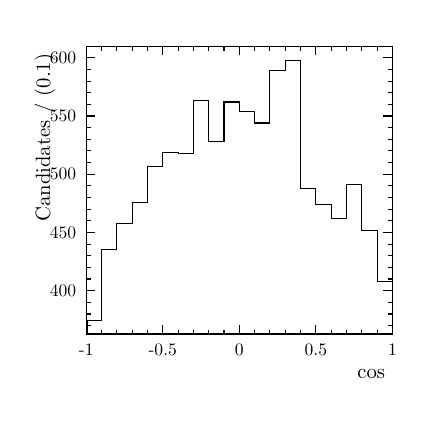
\begin{tikzpicture}
\pgfdeclareplotmark{cross} {
\pgfpathmoveto{\pgfpoint{-0.3\pgfplotmarksize}{\pgfplotmarksize}}
\pgfpathlineto{\pgfpoint{+0.3\pgfplotmarksize}{\pgfplotmarksize}}
\pgfpathlineto{\pgfpoint{+0.3\pgfplotmarksize}{0.3\pgfplotmarksize}}
\pgfpathlineto{\pgfpoint{+1\pgfplotmarksize}{0.3\pgfplotmarksize}}
\pgfpathlineto{\pgfpoint{+1\pgfplotmarksize}{-0.3\pgfplotmarksize}}
\pgfpathlineto{\pgfpoint{+0.3\pgfplotmarksize}{-0.3\pgfplotmarksize}}
\pgfpathlineto{\pgfpoint{+0.3\pgfplotmarksize}{-1.\pgfplotmarksize}}
\pgfpathlineto{\pgfpoint{-0.3\pgfplotmarksize}{-1.\pgfplotmarksize}}
\pgfpathlineto{\pgfpoint{-0.3\pgfplotmarksize}{-0.3\pgfplotmarksize}}
\pgfpathlineto{\pgfpoint{-1.\pgfplotmarksize}{-0.3\pgfplotmarksize}}
\pgfpathlineto{\pgfpoint{-1.\pgfplotmarksize}{0.3\pgfplotmarksize}}
\pgfpathlineto{\pgfpoint{-0.3\pgfplotmarksize}{0.3\pgfplotmarksize}}
\pgfpathclose
\pgfusepathqstroke
}
\pgfdeclareplotmark{cross*} {
\pgfpathmoveto{\pgfpoint{-0.3\pgfplotmarksize}{\pgfplotmarksize}}
\pgfpathlineto{\pgfpoint{+0.3\pgfplotmarksize}{\pgfplotmarksize}}
\pgfpathlineto{\pgfpoint{+0.3\pgfplotmarksize}{0.3\pgfplotmarksize}}
\pgfpathlineto{\pgfpoint{+1\pgfplotmarksize}{0.3\pgfplotmarksize}}
\pgfpathlineto{\pgfpoint{+1\pgfplotmarksize}{-0.3\pgfplotmarksize}}
\pgfpathlineto{\pgfpoint{+0.3\pgfplotmarksize}{-0.3\pgfplotmarksize}}
\pgfpathlineto{\pgfpoint{+0.3\pgfplotmarksize}{-1.\pgfplotmarksize}}
\pgfpathlineto{\pgfpoint{-0.3\pgfplotmarksize}{-1.\pgfplotmarksize}}
\pgfpathlineto{\pgfpoint{-0.3\pgfplotmarksize}{-0.3\pgfplotmarksize}}
\pgfpathlineto{\pgfpoint{-1.\pgfplotmarksize}{-0.3\pgfplotmarksize}}
\pgfpathlineto{\pgfpoint{-1.\pgfplotmarksize}{0.3\pgfplotmarksize}}
\pgfpathlineto{\pgfpoint{-0.3\pgfplotmarksize}{0.3\pgfplotmarksize}}
\pgfpathclose
\pgfusepathqfillstroke
}
\pgfdeclareplotmark{newstar} {
\pgfpathmoveto{\pgfqpoint{0pt}{\pgfplotmarksize}}
\pgfpathlineto{\pgfqpointpolar{44}{0.5\pgfplotmarksize}}
\pgfpathlineto{\pgfqpointpolar{18}{\pgfplotmarksize}}
\pgfpathlineto{\pgfqpointpolar{-20}{0.5\pgfplotmarksize}}
\pgfpathlineto{\pgfqpointpolar{-54}{\pgfplotmarksize}}
\pgfpathlineto{\pgfqpointpolar{-90}{0.5\pgfplotmarksize}}
\pgfpathlineto{\pgfqpointpolar{234}{\pgfplotmarksize}}
\pgfpathlineto{\pgfqpointpolar{198}{0.5\pgfplotmarksize}}
\pgfpathlineto{\pgfqpointpolar{162}{\pgfplotmarksize}}
\pgfpathlineto{\pgfqpointpolar{134}{0.5\pgfplotmarksize}}
\pgfpathclose
\pgfusepathqstroke
}
\pgfdeclareplotmark{newstar*} {
\pgfpathmoveto{\pgfqpoint{0pt}{\pgfplotmarksize}}
\pgfpathlineto{\pgfqpointpolar{44}{0.5\pgfplotmarksize}}
\pgfpathlineto{\pgfqpointpolar{18}{\pgfplotmarksize}}
\pgfpathlineto{\pgfqpointpolar{-20}{0.5\pgfplotmarksize}}
\pgfpathlineto{\pgfqpointpolar{-54}{\pgfplotmarksize}}
\pgfpathlineto{\pgfqpointpolar{-90}{0.5\pgfplotmarksize}}
\pgfpathlineto{\pgfqpointpolar{234}{\pgfplotmarksize}}
\pgfpathlineto{\pgfqpointpolar{198}{0.5\pgfplotmarksize}}
\pgfpathlineto{\pgfqpointpolar{162}{\pgfplotmarksize}}
\pgfpathlineto{\pgfqpointpolar{134}{0.5\pgfplotmarksize}}
\pgfpathclose
\pgfusepathqfillstroke
}
\definecolor{c}{rgb}{1,1,1};
\draw [color=c, fill=c] (0.1,4.91175) rectangle (4.9,9.53456);
\draw [color=c, fill=c] (0.772,5.6514) rectangle (4.66,9.30342);
\definecolor{c}{rgb}{0,0,0};
\draw [c] (0.772,5.6514) -- (0.772,9.30342) -- (4.66,9.30342) -- (4.66,5.6514) -- (0.772,5.6514);
\draw [c,line width=0.4] (0.788779,5.66817) -- (0.788779,5.81702) -- (0.9664,5.81702) -- (0.9664,6.71908) -- (1.1608,6.71908) -- (1.1608,7.05921) -- (1.3552,7.05921) -- (1.3552,7.32539) -- (1.5496,7.32539) -- (1.5496,7.78382) -- (1.744,7.78382) --
 (1.744,7.96127) -- (1.9384,7.96127) -- (1.9384,7.94648) -- (2.1328,7.94648) -- (2.1328,8.61194) -- (2.3272,8.61194) -- (2.3272,8.09436) -- (2.5216,8.09436) -- (2.5216,8.59715) -- (2.716,8.59715) -- (2.716,8.47885) -- (2.9104,8.47885) --
 (2.9104,8.33097) -- (3.1048,8.33097) -- (3.1048,8.99643) -- (3.2992,8.99643) -- (3.2992,9.12952) -- (3.4936,9.12952) -- (3.4936,7.50284) -- (3.688,7.50284) -- (3.688,7.29581) -- (3.8824,7.29581) -- (3.8824,7.11836) -- (4.0768,7.11836) --
 (4.0768,7.54721) -- (4.2712,7.54721) -- (4.2712,6.97048) -- (4.4656,6.97048) -- (4.4656,6.31981) -- (4.66,6.31981) -- (4.66,5.66817);
\draw [c,line width=0.4] (0.772,5.6514) -- (4.66,5.6514);
\draw [anchor= east] (4.66,5.14547) node[scale=0.746701, rotate=0]{$\cos\thetamu$};
\draw [c,line width=0.4] (0.772,5.76373) -- (0.772,5.6514);
\draw [c,line width=0.4] (0.9664,5.70756) -- (0.9664,5.6514);
\draw [c,line width=0.4] (1.1608,5.70756) -- (1.1608,5.6514);
\draw [c,line width=0.4] (1.3552,5.70756) -- (1.3552,5.6514);
\draw [c,line width=0.4] (1.5496,5.70756) -- (1.5496,5.6514);
\draw [c,line width=0.4] (1.744,5.76373) -- (1.744,5.6514);
\draw [c,line width=0.4] (1.9384,5.70756) -- (1.9384,5.6514);
\draw [c,line width=0.4] (2.1328,5.70756) -- (2.1328,5.6514);
\draw [c,line width=0.4] (2.3272,5.70756) -- (2.3272,5.6514);
\draw [c,line width=0.4] (2.5216,5.70756) -- (2.5216,5.6514);
\draw [c,line width=0.4] (2.716,5.76373) -- (2.716,5.6514);
\draw [c,line width=0.4] (2.9104,5.70756) -- (2.9104,5.6514);
\draw [c,line width=0.4] (3.1048,5.70756) -- (3.1048,5.6514);
\draw [c,line width=0.4] (3.2992,5.70756) -- (3.2992,5.6514);
\draw [c,line width=0.4] (3.4936,5.70756) -- (3.4936,5.6514);
\draw [c,line width=0.4] (3.688,5.76373) -- (3.688,5.6514);
\draw [c,line width=0.4] (3.8824,5.70756) -- (3.8824,5.6514);
\draw [c,line width=0.4] (4.0768,5.70756) -- (4.0768,5.6514);
\draw [c,line width=0.4] (4.2712,5.70756) -- (4.2712,5.6514);
\draw [c,line width=0.4] (4.4656,5.70756) -- (4.4656,5.6514);
\draw [c,line width=0.4] (4.66,5.76373) -- (4.66,5.6514);
\draw [anchor=base] (0.772,5.38327) node[scale=0.634696, rotate=0]{-1};
\draw [anchor=base] (1.744,5.38327) node[scale=0.634696, rotate=0]{-0.5};
\draw [anchor=base] (2.716,5.38327) node[scale=0.634696, rotate=0]{0};
\draw [anchor=base] (3.688,5.38327) node[scale=0.634696, rotate=0]{0.5};
\draw [anchor=base] (4.66,5.38327) node[scale=0.634696, rotate=0]{1};
\draw [c,line width=0.4] (0.772,9.30342) -- (4.66,9.30342);
\draw [c,line width=0.4] (0.772,9.19109) -- (0.772,9.30342);
\draw [c,line width=0.4] (0.9664,9.24726) -- (0.9664,9.30342);
\draw [c,line width=0.4] (1.1608,9.24726) -- (1.1608,9.30342);
\draw [c,line width=0.4] (1.3552,9.24726) -- (1.3552,9.30342);
\draw [c,line width=0.4] (1.5496,9.24726) -- (1.5496,9.30342);
\draw [c,line width=0.4] (1.744,9.19109) -- (1.744,9.30342);
\draw [c,line width=0.4] (1.9384,9.24726) -- (1.9384,9.30342);
\draw [c,line width=0.4] (2.1328,9.24726) -- (2.1328,9.30342);
\draw [c,line width=0.4] (2.3272,9.24726) -- (2.3272,9.30342);
\draw [c,line width=0.4] (2.5216,9.24726) -- (2.5216,9.30342);
\draw [c,line width=0.4] (2.716,9.19109) -- (2.716,9.30342);
\draw [c,line width=0.4] (2.9104,9.24726) -- (2.9104,9.30342);
\draw [c,line width=0.4] (3.1048,9.24726) -- (3.1048,9.30342);
\draw [c,line width=0.4] (3.2992,9.24726) -- (3.2992,9.30342);
\draw [c,line width=0.4] (3.4936,9.24726) -- (3.4936,9.30342);
\draw [c,line width=0.4] (3.688,9.19109) -- (3.688,9.30342);
\draw [c,line width=0.4] (3.8824,9.24726) -- (3.8824,9.30342);
\draw [c,line width=0.4] (4.0768,9.24726) -- (4.0768,9.30342);
\draw [c,line width=0.4] (4.2712,9.24726) -- (4.2712,9.30342);
\draw [c,line width=0.4] (4.4656,9.24726) -- (4.4656,9.30342);
\draw [c,line width=0.4] (4.66,9.19109) -- (4.66,9.30342);
\draw [c,line width=0.4] (0.772,5.6514) -- (0.772,9.30342);
\draw [anchor= east] (0.246688,9.30342) node[scale=0.746701, rotate=90]{Candidates / (0.1)};
\draw [c,line width=0.4] (0.88576,6.20151) -- (0.772,6.20151);
\draw [c,line width=0.4] (0.82888,6.34939) -- (0.772,6.34939);
\draw [c,line width=0.4] (0.82888,6.49727) -- (0.772,6.49727);
\draw [c,line width=0.4] (0.82888,6.64514) -- (0.772,6.64514);
\draw [c,line width=0.4] (0.82888,6.79302) -- (0.772,6.79302);
\draw [c,line width=0.4] (0.88576,6.9409) -- (0.772,6.9409);
\draw [c,line width=0.4] (0.82888,7.08878) -- (0.772,7.08878);
\draw [c,line width=0.4] (0.82888,7.23666) -- (0.772,7.23666);
\draw [c,line width=0.4] (0.82888,7.38454) -- (0.772,7.38454);
\draw [c,line width=0.4] (0.82888,7.53242) -- (0.772,7.53242);
\draw [c,line width=0.4] (0.88576,7.6803) -- (0.772,7.6803);
\draw [c,line width=0.4] (0.82888,7.82818) -- (0.772,7.82818);
\draw [c,line width=0.4] (0.82888,7.97606) -- (0.772,7.97606);
\draw [c,line width=0.4] (0.82888,8.12394) -- (0.772,8.12394);
\draw [c,line width=0.4] (0.82888,8.27182) -- (0.772,8.27182);
\draw [c,line width=0.4] (0.88576,8.4197) -- (0.772,8.4197);
\draw [c,line width=0.4] (0.82888,8.56758) -- (0.772,8.56758);
\draw [c,line width=0.4] (0.82888,8.71546) -- (0.772,8.71546);
\draw [c,line width=0.4] (0.82888,8.86333) -- (0.772,8.86333);
\draw [c,line width=0.4] (0.82888,9.01121) -- (0.772,9.01121);
\draw [c,line width=0.4] (0.88576,9.15909) -- (0.772,9.15909);
\draw [c,line width=0.4] (0.88576,6.20151) -- (0.772,6.20151);
\draw [c,line width=0.4] (0.82888,6.05363) -- (0.772,6.05363);
\draw [c,line width=0.4] (0.82888,5.90575) -- (0.772,5.90575);
\draw [c,line width=0.4] (0.82888,5.75787) -- (0.772,5.75787);
\draw [c,line width=0.4] (0.88576,9.15909) -- (0.772,9.15909);
\draw [anchor= east] (0.724,6.20151) node[scale=0.634696, rotate=0]{400};
\draw [anchor= east] (0.724,6.9409) node[scale=0.634696, rotate=0]{450};
\draw [anchor= east] (0.724,7.6803) node[scale=0.634696, rotate=0]{500};
\draw [anchor= east] (0.724,8.4197) node[scale=0.634696, rotate=0]{550};
\draw [anchor= east] (0.724,9.15909) node[scale=0.634696, rotate=0]{600};
\draw [c,line width=0.4] (4.66,5.6514) -- (4.66,9.30342);
\draw [c,line width=0.4] (4.54624,6.20151) -- (4.66,6.20151);
\draw [c,line width=0.4] (4.60312,6.34939) -- (4.66,6.34939);
\draw [c,line width=0.4] (4.60312,6.49727) -- (4.66,6.49727);
\draw [c,line width=0.4] (4.60312,6.64514) -- (4.66,6.64514);
\draw [c,line width=0.4] (4.60312,6.79302) -- (4.66,6.79302);
\draw [c,line width=0.4] (4.54624,6.9409) -- (4.66,6.9409);
\draw [c,line width=0.4] (4.60312,7.08878) -- (4.66,7.08878);
\draw [c,line width=0.4] (4.60312,7.23666) -- (4.66,7.23666);
\draw [c,line width=0.4] (4.60312,7.38454) -- (4.66,7.38454);
\draw [c,line width=0.4] (4.60312,7.53242) -- (4.66,7.53242);
\draw [c,line width=0.4] (4.54624,7.6803) -- (4.66,7.6803);
\draw [c,line width=0.4] (4.60312,7.82818) -- (4.66,7.82818);
\draw [c,line width=0.4] (4.60312,7.97606) -- (4.66,7.97606);
\draw [c,line width=0.4] (4.60312,8.12394) -- (4.66,8.12394);
\draw [c,line width=0.4] (4.60312,8.27182) -- (4.66,8.27182);
\draw [c,line width=0.4] (4.54624,8.4197) -- (4.66,8.4197);
\draw [c,line width=0.4] (4.60312,8.56758) -- (4.66,8.56758);
\draw [c,line width=0.4] (4.60312,8.71546) -- (4.66,8.71546);
\draw [c,line width=0.4] (4.60312,8.86333) -- (4.66,8.86333);
\draw [c,line width=0.4] (4.60312,9.01121) -- (4.66,9.01121);
\draw [c,line width=0.4] (4.54624,9.15909) -- (4.66,9.15909);
\draw [c,line width=0.4] (4.54624,6.20151) -- (4.66,6.20151);
\draw [c,line width=0.4] (4.60312,6.05363) -- (4.66,6.05363);
\draw [c,line width=0.4] (4.60312,5.90575) -- (4.66,5.90575);
\draw [c,line width=0.4] (4.60312,5.75787) -- (4.66,5.75787);
\draw [c,line width=0.4] (4.54624,9.15909) -- (4.66,9.15909);
\end{tikzpicture}
}
    \caption{}
    \label{angDistr_ctl}
  \end{subfigure}%
  \hfill%
  \begin{subfigure}{0.33\textwidth}
    \tikzsetnextfilename{mc_ang_phi}
    \scalebox{0.65}{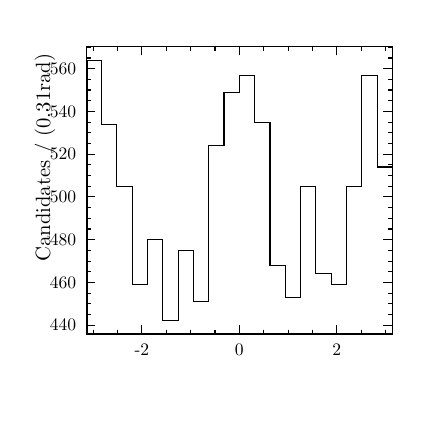
\begin{tikzpicture}
\pgfdeclareplotmark{cross} {
\pgfpathmoveto{\pgfpoint{-0.3\pgfplotmarksize}{\pgfplotmarksize}}
\pgfpathlineto{\pgfpoint{+0.3\pgfplotmarksize}{\pgfplotmarksize}}
\pgfpathlineto{\pgfpoint{+0.3\pgfplotmarksize}{0.3\pgfplotmarksize}}
\pgfpathlineto{\pgfpoint{+1\pgfplotmarksize}{0.3\pgfplotmarksize}}
\pgfpathlineto{\pgfpoint{+1\pgfplotmarksize}{-0.3\pgfplotmarksize}}
\pgfpathlineto{\pgfpoint{+0.3\pgfplotmarksize}{-0.3\pgfplotmarksize}}
\pgfpathlineto{\pgfpoint{+0.3\pgfplotmarksize}{-1.\pgfplotmarksize}}
\pgfpathlineto{\pgfpoint{-0.3\pgfplotmarksize}{-1.\pgfplotmarksize}}
\pgfpathlineto{\pgfpoint{-0.3\pgfplotmarksize}{-0.3\pgfplotmarksize}}
\pgfpathlineto{\pgfpoint{-1.\pgfplotmarksize}{-0.3\pgfplotmarksize}}
\pgfpathlineto{\pgfpoint{-1.\pgfplotmarksize}{0.3\pgfplotmarksize}}
\pgfpathlineto{\pgfpoint{-0.3\pgfplotmarksize}{0.3\pgfplotmarksize}}
\pgfpathclose
\pgfusepathqstroke
}
\pgfdeclareplotmark{cross*} {
\pgfpathmoveto{\pgfpoint{-0.3\pgfplotmarksize}{\pgfplotmarksize}}
\pgfpathlineto{\pgfpoint{+0.3\pgfplotmarksize}{\pgfplotmarksize}}
\pgfpathlineto{\pgfpoint{+0.3\pgfplotmarksize}{0.3\pgfplotmarksize}}
\pgfpathlineto{\pgfpoint{+1\pgfplotmarksize}{0.3\pgfplotmarksize}}
\pgfpathlineto{\pgfpoint{+1\pgfplotmarksize}{-0.3\pgfplotmarksize}}
\pgfpathlineto{\pgfpoint{+0.3\pgfplotmarksize}{-0.3\pgfplotmarksize}}
\pgfpathlineto{\pgfpoint{+0.3\pgfplotmarksize}{-1.\pgfplotmarksize}}
\pgfpathlineto{\pgfpoint{-0.3\pgfplotmarksize}{-1.\pgfplotmarksize}}
\pgfpathlineto{\pgfpoint{-0.3\pgfplotmarksize}{-0.3\pgfplotmarksize}}
\pgfpathlineto{\pgfpoint{-1.\pgfplotmarksize}{-0.3\pgfplotmarksize}}
\pgfpathlineto{\pgfpoint{-1.\pgfplotmarksize}{0.3\pgfplotmarksize}}
\pgfpathlineto{\pgfpoint{-0.3\pgfplotmarksize}{0.3\pgfplotmarksize}}
\pgfpathclose
\pgfusepathqfillstroke
}
\pgfdeclareplotmark{newstar} {
\pgfpathmoveto{\pgfqpoint{0pt}{\pgfplotmarksize}}
\pgfpathlineto{\pgfqpointpolar{44}{0.5\pgfplotmarksize}}
\pgfpathlineto{\pgfqpointpolar{18}{\pgfplotmarksize}}
\pgfpathlineto{\pgfqpointpolar{-20}{0.5\pgfplotmarksize}}
\pgfpathlineto{\pgfqpointpolar{-54}{\pgfplotmarksize}}
\pgfpathlineto{\pgfqpointpolar{-90}{0.5\pgfplotmarksize}}
\pgfpathlineto{\pgfqpointpolar{234}{\pgfplotmarksize}}
\pgfpathlineto{\pgfqpointpolar{198}{0.5\pgfplotmarksize}}
\pgfpathlineto{\pgfqpointpolar{162}{\pgfplotmarksize}}
\pgfpathlineto{\pgfqpointpolar{134}{0.5\pgfplotmarksize}}
\pgfpathclose
\pgfusepathqstroke
}
\pgfdeclareplotmark{newstar*} {
\pgfpathmoveto{\pgfqpoint{0pt}{\pgfplotmarksize}}
\pgfpathlineto{\pgfqpointpolar{44}{0.5\pgfplotmarksize}}
\pgfpathlineto{\pgfqpointpolar{18}{\pgfplotmarksize}}
\pgfpathlineto{\pgfqpointpolar{-20}{0.5\pgfplotmarksize}}
\pgfpathlineto{\pgfqpointpolar{-54}{\pgfplotmarksize}}
\pgfpathlineto{\pgfqpointpolar{-90}{0.5\pgfplotmarksize}}
\pgfpathlineto{\pgfqpointpolar{234}{\pgfplotmarksize}}
\pgfpathlineto{\pgfqpointpolar{198}{0.5\pgfplotmarksize}}
\pgfpathlineto{\pgfqpointpolar{162}{\pgfplotmarksize}}
\pgfpathlineto{\pgfqpointpolar{134}{0.5\pgfplotmarksize}}
\pgfpathclose
\pgfusepathqfillstroke
}
\definecolor{c}{rgb}{1,1,1};
\draw [color=c, fill=c] (5.1,4.91175) rectangle (9.9,9.53456);
\draw [color=c, fill=c] (5.772,5.6514) rectangle (9.66,9.30342);
\definecolor{c}{rgb}{0,0,0};
\draw [c] (5.772,5.6514) -- (5.772,9.30342) -- (9.66,9.30342) -- (9.66,5.6514) -- (5.772,5.6514);
\draw [c,line width=0.4] (5.78878,5.66817) -- (5.78878,9.12952) -- (5.9664,9.12952) -- (5.9664,8.31497) -- (6.1608,8.31497) -- (6.1608,7.52757) -- (6.3552,7.52757) -- (6.3552,6.2786) -- (6.5496,6.2786) -- (6.5496,6.84878) -- (6.744,6.84878) --
 (6.744,5.81702) -- (6.9384,5.81702) -- (6.9384,6.71302) -- (7.1328,6.71302) -- (7.1328,6.06139) -- (7.3272,6.06139) -- (7.3272,8.04345) -- (7.5216,8.04345) -- (7.5216,8.72224) -- (7.716,8.72224) -- (7.716,8.93946) -- (7.9104,8.93946) --
 (7.9104,8.34212) -- (8.1048,8.34212) -- (8.1048,6.52296) -- (8.2992,6.52296) -- (8.2992,6.11569) -- (8.4936,6.11569) -- (8.4936,7.52757) -- (8.688,7.52757) -- (8.688,6.41436) -- (8.8824,6.41436) -- (8.8824,6.2786) -- (9.0768,6.2786) --
 (9.0768,7.52757) -- (9.2712,7.52757) -- (9.2712,8.93946) -- (9.4656,8.93946) -- (9.4656,7.77194) -- (9.66,7.77194);
\draw [c,line width=0.4] (5.772,5.6514) -- (9.66,5.6514);
\draw [anchor= east] (9.66,5.14547) node[scale=0.746701, rotate=0]{$\phihel$};
\draw [c,line width=0.4] (6.47841,5.76373) -- (6.47841,5.6514);
\draw [c,line width=0.4] (6.78781,5.70756) -- (6.78781,5.6514);
\draw [c,line width=0.4] (7.09721,5.70756) -- (7.09721,5.6514);
\draw [c,line width=0.4] (7.4066,5.70756) -- (7.4066,5.6514);
\draw [c,line width=0.4] (7.716,5.76373) -- (7.716,5.6514);
\draw [c,line width=0.4] (8.0254,5.70756) -- (8.0254,5.6514);
\draw [c,line width=0.4] (8.33479,5.70756) -- (8.33479,5.6514);
\draw [c,line width=0.4] (8.64419,5.70756) -- (8.64419,5.6514);
\draw [c,line width=0.4] (8.95359,5.76373) -- (8.95359,5.6514);
\draw [c,line width=0.4] (6.47841,5.76373) -- (6.47841,5.6514);
\draw [c,line width=0.4] (6.16901,5.70756) -- (6.16901,5.6514);
\draw [c,line width=0.4] (5.85962,5.70756) -- (5.85962,5.6514);
\draw [c,line width=0.4] (8.95359,5.76373) -- (8.95359,5.6514);
\draw [c,line width=0.4] (9.26299,5.70756) -- (9.26299,5.6514);
\draw [c,line width=0.4] (9.57238,5.70756) -- (9.57238,5.6514);
\draw [anchor=base] (6.47841,5.38327) node[scale=0.634696, rotate=0]{-2};
\draw [anchor=base] (7.716,5.38327) node[scale=0.634696, rotate=0]{0};
\draw [anchor=base] (8.95359,5.38327) node[scale=0.634696, rotate=0]{2};
\draw [c,line width=0.4] (5.772,9.30342) -- (9.66,9.30342);
\draw [c,line width=0.4] (6.47841,9.19109) -- (6.47841,9.30342);
\draw [c,line width=0.4] (6.78781,9.24726) -- (6.78781,9.30342);
\draw [c,line width=0.4] (7.09721,9.24726) -- (7.09721,9.30342);
\draw [c,line width=0.4] (7.4066,9.24726) -- (7.4066,9.30342);
\draw [c,line width=0.4] (7.716,9.19109) -- (7.716,9.30342);
\draw [c,line width=0.4] (8.0254,9.24726) -- (8.0254,9.30342);
\draw [c,line width=0.4] (8.33479,9.24726) -- (8.33479,9.30342);
\draw [c,line width=0.4] (8.64419,9.24726) -- (8.64419,9.30342);
\draw [c,line width=0.4] (8.95359,9.19109) -- (8.95359,9.30342);
\draw [c,line width=0.4] (6.47841,9.19109) -- (6.47841,9.30342);
\draw [c,line width=0.4] (6.16901,9.24726) -- (6.16901,9.30342);
\draw [c,line width=0.4] (5.85962,9.24726) -- (5.85962,9.30342);
\draw [c,line width=0.4] (8.95359,9.19109) -- (8.95359,9.30342);
\draw [c,line width=0.4] (9.26299,9.24726) -- (9.26299,9.30342);
\draw [c,line width=0.4] (9.57238,9.24726) -- (9.57238,9.30342);
\draw [c,line width=0.4] (5.772,5.6514) -- (5.772,9.30342);
\draw [anchor= east] (5.24669,9.30342) node[scale=0.746701, rotate=90]{Candidates / (0.31rad)};
\draw [c,line width=0.4] (5.88576,5.76272) -- (5.772,5.76272);
\draw [c,line width=0.4] (5.82888,5.89848) -- (5.772,5.89848);
\draw [c,line width=0.4] (5.82888,6.03423) -- (5.772,6.03423);
\draw [c,line width=0.4] (5.82888,6.16999) -- (5.772,6.16999);
\draw [c,line width=0.4] (5.88576,6.30575) -- (5.772,6.30575);
\draw [c,line width=0.4] (5.82888,6.44151) -- (5.772,6.44151);
\draw [c,line width=0.4] (5.82888,6.57727) -- (5.772,6.57727);
\draw [c,line width=0.4] (5.82888,6.71302) -- (5.772,6.71302);
\draw [c,line width=0.4] (5.88576,6.84878) -- (5.772,6.84878);
\draw [c,line width=0.4] (5.82888,6.98454) -- (5.772,6.98454);
\draw [c,line width=0.4] (5.82888,7.1203) -- (5.772,7.1203);
\draw [c,line width=0.4] (5.82888,7.25606) -- (5.772,7.25606);
\draw [c,line width=0.4] (5.88576,7.39181) -- (5.772,7.39181);
\draw [c,line width=0.4] (5.82888,7.52757) -- (5.772,7.52757);
\draw [c,line width=0.4] (5.82888,7.66333) -- (5.772,7.66333);
\draw [c,line width=0.4] (5.82888,7.79909) -- (5.772,7.79909);
\draw [c,line width=0.4] (5.88576,7.93485) -- (5.772,7.93485);
\draw [c,line width=0.4] (5.82888,8.0706) -- (5.772,8.0706);
\draw [c,line width=0.4] (5.82888,8.20636) -- (5.772,8.20636);
\draw [c,line width=0.4] (5.82888,8.34212) -- (5.772,8.34212);
\draw [c,line width=0.4] (5.88576,8.47788) -- (5.772,8.47788);
\draw [c,line width=0.4] (5.82888,8.61364) -- (5.772,8.61364);
\draw [c,line width=0.4] (5.82888,8.74939) -- (5.772,8.74939);
\draw [c,line width=0.4] (5.82888,8.88515) -- (5.772,8.88515);
\draw [c,line width=0.4] (5.88576,9.02091) -- (5.772,9.02091);
\draw [c,line width=0.4] (5.88576,5.76272) -- (5.772,5.76272);
\draw [c,line width=0.4] (5.88576,9.02091) -- (5.772,9.02091);
\draw [c,line width=0.4] (5.82888,9.15667) -- (5.772,9.15667);
\draw [c,line width=0.4] (5.82888,9.29243) -- (5.772,9.29243);
\draw [anchor= east] (5.724,5.76272) node[scale=0.634696, rotate=0]{440};
\draw [anchor= east] (5.724,6.30575) node[scale=0.634696, rotate=0]{460};
\draw [anchor= east] (5.724,6.84878) node[scale=0.634696, rotate=0]{480};
\draw [anchor= east] (5.724,7.39181) node[scale=0.634696, rotate=0]{500};
\draw [anchor= east] (5.724,7.93485) node[scale=0.634696, rotate=0]{520};
\draw [anchor= east] (5.724,8.47788) node[scale=0.634696, rotate=0]{540};
\draw [anchor= east] (5.724,9.02091) node[scale=0.634696, rotate=0]{560};
\draw [c,line width=0.4] (9.66,5.6514) -- (9.66,9.30342);
\draw [c,line width=0.4] (9.54624,5.76272) -- (9.66,5.76272);
\draw [c,line width=0.4] (9.60312,5.89848) -- (9.66,5.89848);
\draw [c,line width=0.4] (9.60312,6.03423) -- (9.66,6.03423);
\draw [c,line width=0.4] (9.60312,6.16999) -- (9.66,6.16999);
\draw [c,line width=0.4] (9.54624,6.30575) -- (9.66,6.30575);
\draw [c,line width=0.4] (9.60312,6.44151) -- (9.66,6.44151);
\draw [c,line width=0.4] (9.60312,6.57727) -- (9.66,6.57727);
\draw [c,line width=0.4] (9.60312,6.71302) -- (9.66,6.71302);
\draw [c,line width=0.4] (9.54624,6.84878) -- (9.66,6.84878);
\draw [c,line width=0.4] (9.60312,6.98454) -- (9.66,6.98454);
\draw [c,line width=0.4] (9.60312,7.1203) -- (9.66,7.1203);
\draw [c,line width=0.4] (9.60312,7.25606) -- (9.66,7.25606);
\draw [c,line width=0.4] (9.54624,7.39181) -- (9.66,7.39181);
\draw [c,line width=0.4] (9.60312,7.52757) -- (9.66,7.52757);
\draw [c,line width=0.4] (9.60312,7.66333) -- (9.66,7.66333);
\draw [c,line width=0.4] (9.60312,7.79909) -- (9.66,7.79909);
\draw [c,line width=0.4] (9.54624,7.93485) -- (9.66,7.93485);
\draw [c,line width=0.4] (9.60312,8.0706) -- (9.66,8.0706);
\draw [c,line width=0.4] (9.60312,8.20636) -- (9.66,8.20636);
\draw [c,line width=0.4] (9.60312,8.34212) -- (9.66,8.34212);
\draw [c,line width=0.4] (9.54624,8.47788) -- (9.66,8.47788);
\draw [c,line width=0.4] (9.60312,8.61364) -- (9.66,8.61364);
\draw [c,line width=0.4] (9.60312,8.74939) -- (9.66,8.74939);
\draw [c,line width=0.4] (9.60312,8.88515) -- (9.66,8.88515);
\draw [c,line width=0.4] (9.54624,9.02091) -- (9.66,9.02091);
\draw [c,line width=0.4] (9.54624,5.76272) -- (9.66,5.76272);
\draw [c,line width=0.4] (9.54624,9.02091) -- (9.66,9.02091);
\draw [c,line width=0.4] (9.60312,9.15667) -- (9.66,9.15667);
\draw [c,line width=0.4] (9.60312,9.29243) -- (9.66,9.29243);
\end{tikzpicture}
}
    \caption{}
    \label{angDistr_phi}
  \end{subfigure}
  \caption{Decay angles distributions from simulation data. No detector effects and no selection are included.
           Histograms are normalized to unity area.}
  \label{angDistr_all}
\end{figure}

The above situation is related to kinematic constrains in two body decays particularly close to phase
space boundaries. The latter constraint manifests itself when computing the angle of the pion
with respect to the boost direction in the lab frame, as shown in the following equation:

\begin{equation}
  \centering
  \tan\thetapi^\lab = \frac{\ptrans{\pi}^\lab}{\plongd{\pi}^\lab}
               = \frac{\ptrans{\pi}}{\gamma\parenthesis{\plongd{\pi} + \beta E_\pi} }
               = \frac{\ptot_{\pi} \sin\thetapi}{\gamma\parenthesis{\ptot_{\pi} \cos\thetapi + \beta E_\pi} },
  \label{pi_angle}
\end{equation}

\begin{figure}[t]
  \centering
  \begin{subfigure}{0.49\textwidth}
    \raggedright
    \tikzsetnextfilename{ctk_kaon_kaon_pt}
    \scalebox{1.15}{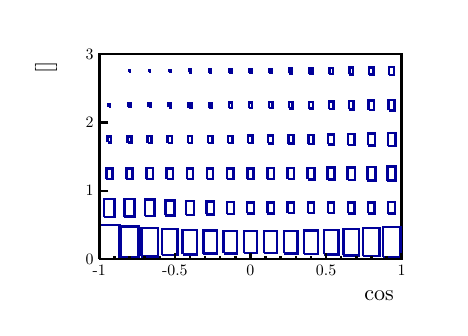
\begin{tikzpicture}
\pgfdeclareplotmark{cross} {
\pgfpathmoveto{\pgfpoint{-0.3\pgfplotmarksize}{\pgfplotmarksize}}
\pgfpathlineto{\pgfpoint{+0.3\pgfplotmarksize}{\pgfplotmarksize}}
\pgfpathlineto{\pgfpoint{+0.3\pgfplotmarksize}{0.3\pgfplotmarksize}}
\pgfpathlineto{\pgfpoint{+1\pgfplotmarksize}{0.3\pgfplotmarksize}}
\pgfpathlineto{\pgfpoint{+1\pgfplotmarksize}{-0.3\pgfplotmarksize}}
\pgfpathlineto{\pgfpoint{+0.3\pgfplotmarksize}{-0.3\pgfplotmarksize}}
\pgfpathlineto{\pgfpoint{+0.3\pgfplotmarksize}{-1.\pgfplotmarksize}}
\pgfpathlineto{\pgfpoint{-0.3\pgfplotmarksize}{-1.\pgfplotmarksize}}
\pgfpathlineto{\pgfpoint{-0.3\pgfplotmarksize}{-0.3\pgfplotmarksize}}
\pgfpathlineto{\pgfpoint{-1.\pgfplotmarksize}{-0.3\pgfplotmarksize}}
\pgfpathlineto{\pgfpoint{-1.\pgfplotmarksize}{0.3\pgfplotmarksize}}
\pgfpathlineto{\pgfpoint{-0.3\pgfplotmarksize}{0.3\pgfplotmarksize}}
\pgfpathclose
\pgfusepathqstroke
}
\pgfdeclareplotmark{cross*} {
\pgfpathmoveto{\pgfpoint{-0.3\pgfplotmarksize}{\pgfplotmarksize}}
\pgfpathlineto{\pgfpoint{+0.3\pgfplotmarksize}{\pgfplotmarksize}}
\pgfpathlineto{\pgfpoint{+0.3\pgfplotmarksize}{0.3\pgfplotmarksize}}
\pgfpathlineto{\pgfpoint{+1\pgfplotmarksize}{0.3\pgfplotmarksize}}
\pgfpathlineto{\pgfpoint{+1\pgfplotmarksize}{-0.3\pgfplotmarksize}}
\pgfpathlineto{\pgfpoint{+0.3\pgfplotmarksize}{-0.3\pgfplotmarksize}}
\pgfpathlineto{\pgfpoint{+0.3\pgfplotmarksize}{-1.\pgfplotmarksize}}
\pgfpathlineto{\pgfpoint{-0.3\pgfplotmarksize}{-1.\pgfplotmarksize}}
\pgfpathlineto{\pgfpoint{-0.3\pgfplotmarksize}{-0.3\pgfplotmarksize}}
\pgfpathlineto{\pgfpoint{-1.\pgfplotmarksize}{-0.3\pgfplotmarksize}}
\pgfpathlineto{\pgfpoint{-1.\pgfplotmarksize}{0.3\pgfplotmarksize}}
\pgfpathlineto{\pgfpoint{-0.3\pgfplotmarksize}{0.3\pgfplotmarksize}}
\pgfpathclose
\pgfusepathqfillstroke
}
\pgfdeclareplotmark{newstar} {
\pgfpathmoveto{\pgfqpoint{0pt}{\pgfplotmarksize}}
\pgfpathlineto{\pgfqpointpolar{44}{0.5\pgfplotmarksize}}
\pgfpathlineto{\pgfqpointpolar{18}{\pgfplotmarksize}}
\pgfpathlineto{\pgfqpointpolar{-20}{0.5\pgfplotmarksize}}
\pgfpathlineto{\pgfqpointpolar{-54}{\pgfplotmarksize}}
\pgfpathlineto{\pgfqpointpolar{-90}{0.5\pgfplotmarksize}}
\pgfpathlineto{\pgfqpointpolar{234}{\pgfplotmarksize}}
\pgfpathlineto{\pgfqpointpolar{198}{0.5\pgfplotmarksize}}
\pgfpathlineto{\pgfqpointpolar{162}{\pgfplotmarksize}}
\pgfpathlineto{\pgfqpointpolar{134}{0.5\pgfplotmarksize}}
\pgfpathclose
\pgfusepathqstroke
}
\pgfdeclareplotmark{newstar*} {
\pgfpathmoveto{\pgfqpoint{0pt}{\pgfplotmarksize}}
\pgfpathlineto{\pgfqpointpolar{44}{0.5\pgfplotmarksize}}
\pgfpathlineto{\pgfqpointpolar{18}{\pgfplotmarksize}}
\pgfpathlineto{\pgfqpointpolar{-20}{0.5\pgfplotmarksize}}
\pgfpathlineto{\pgfqpointpolar{-54}{\pgfplotmarksize}}
\pgfpathlineto{\pgfqpointpolar{-90}{0.5\pgfplotmarksize}}
\pgfpathlineto{\pgfqpointpolar{234}{\pgfplotmarksize}}
\pgfpathlineto{\pgfqpointpolar{198}{0.5\pgfplotmarksize}}
\pgfpathlineto{\pgfqpointpolar{162}{\pgfplotmarksize}}
\pgfpathlineto{\pgfqpointpolar{134}{0.5\pgfplotmarksize}}
\pgfpathclose
\pgfusepathqfillstroke
}
\definecolor{c}{rgb}{1,1,1};
\draw [color=c, fill=c] (0.1,3.46332) rectangle (4.9,6.72292);
\draw [color=c, fill=c] (0.58,3.78928) rectangle (4.42,6.39696);
\definecolor{c}{rgb}{0,0,0};
\draw [c,line width=0.9] (0.58,3.78928) -- (0.58,6.39696) -- (4.42,6.39696) -- (4.42,3.78928) -- (0.58,3.78928);
\definecolor{c}{rgb}{0,0,0.6};
\draw [c,line width=0.9] (0.58,3.78928) -- (0.58,4.2239) -- (0.836,4.2239) -- (0.836,3.78928) -- (0.58,3.78928);
\draw [c,line width=0.9] (0.84733,3.80852) -- (0.84733,4.20466) -- (1.08067,4.20466) -- (1.08067,3.80852) -- (0.84733,3.80852);
\draw [c,line width=0.9] (1.11404,3.8267) -- (1.11404,4.18648) -- (1.32596,4.18648) -- (1.32596,3.8267) -- (1.11404,3.8267);
\draw [c,line width=0.9] (1.3777,3.8397) -- (1.3777,4.17348) -- (1.5743,4.17348) -- (1.5743,3.8397) -- (1.3777,3.8397);
\draw [c,line width=0.9] (1.63999,3.85039) -- (1.63999,4.1628) -- (1.82401,4.1628) -- (1.82401,3.85039) -- (1.63999,3.85039);
\draw [c,line width=0.9] (1.90111,3.85907) -- (1.90111,4.15411) -- (2.07489,4.15411) -- (2.07489,3.85907) -- (1.90111,3.85907);
\draw [c,line width=0.9] (2.16018,3.86429) -- (2.16018,4.14889) -- (2.32782,4.14889) -- (2.32782,3.86429) -- (2.16018,3.86429);
\draw [c,line width=0.9] (2.41738,3.86632) -- (2.41738,4.14686) -- (2.58262,4.14686) -- (2.58262,3.86632) -- (2.41738,3.86632);
\draw [c,line width=0.9] (2.67349,3.86652) -- (2.67349,4.14666) -- (2.83851,4.14666) -- (2.83851,3.86652) -- (2.67349,3.86652);
\draw [c,line width=0.9] (2.92746,3.86307) -- (2.92746,4.15011) -- (3.09654,4.15011) -- (3.09654,3.86307) -- (2.92746,3.86307);
\draw [c,line width=0.9] (3.18025,3.85761) -- (3.18025,4.15557) -- (3.35575,4.15557) -- (3.35575,3.85761) -- (3.18025,3.85761);
\draw [c,line width=0.9] (3.4319,3.85023) -- (3.4319,4.16295) -- (3.6161,4.16295) -- (3.6161,3.85023) -- (3.4319,3.85023);
\draw [c,line width=0.9] (3.68148,3.83933) -- (3.68148,4.17385) -- (3.87852,4.17385) -- (3.87852,3.83933) -- (3.68148,3.83933);
\draw [c,line width=0.9] (3.9315,3.82918) -- (3.9315,4.184) -- (4.1405,4.184) -- (4.1405,3.82918) -- (3.9315,3.82918);
\draw [c,line width=0.9] (4.18015,3.81671) -- (4.18015,4.19648) -- (4.40385,4.19648) -- (4.40385,3.81671) -- (4.18015,3.81671);
\draw [c,line width=0.9] (0.64082,4.32715) -- (0.64082,4.55526) -- (0.77518,4.55526) -- (0.77518,4.32715) -- (0.64082,4.32715);
\draw [c,line width=0.9] (0.899106,4.33103) -- (0.899106,4.55137) -- (1.02889,4.55137) -- (1.02889,4.33103) -- (0.899106,4.33103);
\draw [c,line width=0.9] (1.15909,4.33779) -- (1.15909,4.54462) -- (1.28091,4.54462) -- (1.28091,4.33779) -- (1.15909,4.33779);
\draw [c,line width=0.9] (1.41921,4.34479) -- (1.41921,4.53761) -- (1.53279,4.53761) -- (1.53279,4.34479) -- (1.41921,4.34479);
\draw [c,line width=0.9] (1.67964,4.35231) -- (1.67964,4.5301) -- (1.78436,4.5301) -- (1.78436,4.35231) -- (1.67964,4.35231);
\draw [c,line width=0.9] (1.93958,4.35901) -- (1.93958,4.5234) -- (2.03642,4.5234) -- (2.03642,4.35901) -- (1.93958,4.35901);
\draw [c,line width=0.9] (2.19924,4.36521) -- (2.19924,4.5172) -- (2.28876,4.5172) -- (2.28876,4.36521) -- (2.19924,4.36521);
\draw [c,line width=0.9] (2.45814,4.37014) -- (2.45814,4.51227) -- (2.54186,4.51227) -- (2.54186,4.37014) -- (2.45814,4.37014);
\draw [c,line width=0.9] (2.71575,4.37288) -- (2.71575,4.50953) -- (2.79625,4.50953) -- (2.79625,4.37288) -- (2.71575,4.37288);
\draw [c,line width=0.9] (2.97247,4.3741) -- (2.97247,4.50831) -- (3.05153,4.50831) -- (3.05153,4.3741) -- (2.97247,4.3741);
\draw [c,line width=0.9] (3.22831,4.37382) -- (3.22831,4.50859) -- (3.30769,4.50859) -- (3.30769,4.37382) -- (3.22831,4.37382);
\draw [c,line width=0.9] (3.48439,4.37396) -- (3.48439,4.50845) -- (3.56361,4.50845) -- (3.56361,4.37396) -- (3.48439,4.37396);
\draw [c,line width=0.9] (3.73979,4.37294) -- (3.73979,4.50947) -- (3.82021,4.50947) -- (3.82021,4.37294) -- (3.73979,4.37294);
\draw [c,line width=0.9] (3.9945,4.37075) -- (3.9945,4.51165) -- (4.0775,4.51165) -- (4.0775,4.37075) -- (3.9945,4.37075);
\draw [c,line width=0.9] (4.2497,4.36939) -- (4.2497,4.51302) -- (4.3343,4.51302) -- (4.3343,4.36939) -- (4.2497,4.36939);
\draw [c,line width=0.9] (0.669015,4.80963) -- (0.669015,4.942) -- (0.746985,4.942) -- (0.746985,4.80963) -- (0.669015,4.80963);
\draw [c,line width=0.9] (0.923694,4.80739) -- (0.923694,4.94424) -- (1.00431,4.94424) -- (1.00431,4.80739) -- (0.923694,4.80739);
\draw [c,line width=0.9] (1.17945,4.80698) -- (1.17945,4.94466) -- (1.26055,4.94466) -- (1.26055,4.80698) -- (1.17945,4.80698);
\draw [c,line width=0.9] (1.43623,4.80829) -- (1.43623,4.94334) -- (1.51577,4.94334) -- (1.51577,4.80829) -- (1.43623,4.80829);
\draw [c,line width=0.9] (1.69297,4.80955) -- (1.69297,4.94208) -- (1.77103,4.94208) -- (1.77103,4.80955) -- (1.69297,4.80955);
\draw [c,line width=0.9] (1.94913,4.80983) -- (1.94913,4.9418) -- (2.02687,4.9418) -- (2.02687,4.80983) -- (1.94913,4.80983);
\draw [c,line width=0.9] (2.20509,4.80976) -- (2.20509,4.94188) -- (2.28291,4.94188) -- (2.28291,4.80976) -- (2.20509,4.80976);
\draw [c,line width=0.9] (2.46024,4.80832) -- (2.46024,4.94332) -- (2.53976,4.94332) -- (2.53976,4.80832) -- (2.46024,4.80832);
\draw [c,line width=0.9] (2.71526,4.80665) -- (2.71526,4.94498) -- (2.79674,4.94498) -- (2.79674,4.80665) -- (2.71526,4.80665);
\draw [c,line width=0.9] (2.97048,4.80533) -- (2.97048,4.94631) -- (3.05352,4.94631) -- (3.05352,4.80533) -- (2.97048,4.80533);
\draw [c,line width=0.9] (3.22504,4.80288) -- (3.22504,4.94876) -- (3.31096,4.94876) -- (3.31096,4.80288) -- (3.22504,4.80288);
\draw [c,line width=0.9] (3.47859,4.79873) -- (3.47859,4.95291) -- (3.56941,4.95291) -- (3.56941,4.79873) -- (3.47859,4.79873);
\draw [c,line width=0.9] (3.73304,4.79609) -- (3.73304,4.95555) -- (3.82696,4.95555) -- (3.82696,4.79609) -- (3.73304,4.79609);
\draw [c,line width=0.9] (3.98638,4.79158) -- (3.98638,4.96005) -- (4.08562,4.96005) -- (4.08562,4.79158) -- (3.98638,4.79158);
\draw [c,line width=0.9] (4.23997,4.78749) -- (4.23997,4.96414) -- (4.34403,4.96414) -- (4.34403,4.78749) -- (4.23997,4.78749);
\draw [c,line width=0.9] (0.68646,5.27386) -- (0.68646,5.347) -- (0.72954,5.347) -- (0.72954,5.27386) -- (0.68646,5.27386);
\draw [c,line width=0.9] (0.940401,5.27037) -- (0.940401,5.35049) -- (0.987599,5.35049) -- (0.987599,5.27037) -- (0.940401,5.27037);
\draw [c,line width=0.9] (1.19468,5.26744) -- (1.19468,5.35342) -- (1.24532,5.35342) -- (1.24532,5.26744) -- (1.19468,5.26744);
\draw [c,line width=0.9] (1.44956,5.26555) -- (1.44956,5.35531) -- (1.50244,5.35531) -- (1.50244,5.26555) -- (1.44956,5.26555);
\draw [c,line width=0.9] (1.70513,5.26481) -- (1.70513,5.35605) -- (1.75887,5.35605) -- (1.75887,5.26481) -- (1.70513,5.26481);
\draw [c,line width=0.9] (1.961,5.2646) -- (1.961,5.35626) -- (2.015,5.35626) -- (2.015,5.2646) -- (1.961,5.2646);
\draw [c,line width=0.9] (2.21669,5.26407) -- (2.21669,5.35679) -- (2.27131,5.35679) -- (2.27131,5.26407) -- (2.21669,5.26407);
\draw [c,line width=0.9] (2.47152,5.26209) -- (2.47152,5.35877) -- (2.52848,5.35877) -- (2.52848,5.26209) -- (2.47152,5.26209);
\draw [c,line width=0.9] (2.72589,5.25932) -- (2.72589,5.36154) -- (2.78611,5.36154) -- (2.78611,5.25932) -- (2.72589,5.25932);
\draw [c,line width=0.9] (2.98046,5.25689) -- (2.98046,5.36397) -- (3.04354,5.36397) -- (3.04354,5.25689) -- (2.98046,5.25689);
\draw [c,line width=0.9] (3.23427,5.25317) -- (3.23427,5.36769) -- (3.30173,5.36769) -- (3.30173,5.25317) -- (3.23427,5.25317);
\draw [c,line width=0.9] (3.48734,5.2482) -- (3.48734,5.37266) -- (3.56066,5.37266) -- (3.56066,5.2482) -- (3.48734,5.2482);
\draw [c,line width=0.9] (3.73948,5.24164) -- (3.73948,5.37922) -- (3.82052,5.37922) -- (3.82052,5.24164) -- (3.73948,5.24164);
\draw [c,line width=0.9] (3.99195,5.23565) -- (3.99195,5.38521) -- (4.08005,5.38521) -- (4.08005,5.23565) -- (3.99195,5.23565);
\draw [c,line width=0.9] (4.2448,5.23029) -- (4.2448,5.39057) -- (4.3392,5.39057) -- (4.3392,5.23029) -- (4.2448,5.23029);
\draw [c,line width=0.9] (0.697728,5.7276) -- (0.697728,5.76248) -- (0.718272,5.76248) -- (0.718272,5.7276) -- (0.697728,5.7276);
\draw [c,line width=0.9] (0.950787,5.72261) -- (0.950787,5.76748) -- (0.977213,5.76748) -- (0.977213,5.72261) -- (0.950787,5.72261);
\draw [c,line width=0.9] (1.20558,5.72056) -- (1.20558,5.76953) -- (1.23442,5.76953) -- (1.23442,5.72056) -- (1.20558,5.72056);
\draw [c,line width=0.9] (1.45953,5.71708) -- (1.45953,5.77301) -- (1.49247,5.77301) -- (1.49247,5.71708) -- (1.45953,5.71708);
\draw [c,line width=0.9] (1.71432,5.71503) -- (1.71432,5.77505) -- (1.74968,5.77505) -- (1.74968,5.71503) -- (1.71432,5.71503);
\draw [c,line width=0.9] (1.97034,5.71507) -- (1.97034,5.77502) -- (2.00566,5.77502) -- (2.00566,5.71507) -- (1.97034,5.71507);
\draw [c,line width=0.9] (2.22429,5.71159) -- (2.22429,5.7785) -- (2.26371,5.7785) -- (2.26371,5.71159) -- (2.22429,5.71159);
\draw [c,line width=0.9] (2.47907,5.70952) -- (2.47907,5.78057) -- (2.52093,5.78057) -- (2.52093,5.70952) -- (2.47907,5.70952);
\draw [c,line width=0.9] (2.73351,5.70686) -- (2.73351,5.78323) -- (2.77849,5.78323) -- (2.77849,5.70686) -- (2.73351,5.70686);
\draw [c,line width=0.9] (2.98764,5.70368) -- (2.98764,5.78641) -- (3.03636,5.78641) -- (3.03636,5.70368) -- (2.98764,5.70368);
\draw [c,line width=0.9] (3.24236,5.70152) -- (3.24236,5.78856) -- (3.29364,5.78856) -- (3.29364,5.70152) -- (3.24236,5.70152);
\draw [c,line width=0.9] (3.49636,5.69812) -- (3.49636,5.79197) -- (3.55164,5.79197) -- (3.55164,5.69812) -- (3.49636,5.69812);
\draw [c,line width=0.9] (3.74886,5.69218) -- (3.74886,5.79791) -- (3.81114,5.79791) -- (3.81114,5.69218) -- (3.74886,5.69218);
\draw [c,line width=0.9] (4.00158,5.6866) -- (4.00158,5.80348) -- (4.07042,5.80348) -- (4.07042,5.6866) -- (4.00158,5.6866);
\draw [c,line width=0.9] (4.2543,5.68104) -- (4.2543,5.80905) -- (4.3297,5.80905) -- (4.3297,5.68104) -- (4.2543,5.68104);
\draw [c,line width=0.9] (0.959602,6.17219) -- (0.959602,6.18712) -- (0.968398,6.18712) -- (0.968398,6.17219) -- (0.959602,6.17219);
\draw [c,line width=0.9] (1.21329,6.16827) -- (1.21329,6.19104) -- (1.22671,6.19104) -- (1.22671,6.16827) -- (1.21329,6.16827);
\draw [c,line width=0.9] (1.4676,6.16539) -- (1.4676,6.19392) -- (1.4844,6.19392) -- (1.4844,6.16539) -- (1.4676,6.16539);
\draw [c,line width=0.9] (1.72204,6.16274) -- (1.72204,6.19657) -- (1.74196,6.19657) -- (1.74196,6.16274) -- (1.72204,6.16274);
\draw [c,line width=0.9] (1.97651,6.16014) -- (1.97651,6.19917) -- (1.9995,6.19917) -- (1.9995,6.16014) -- (1.97651,6.16014);
\draw [c,line width=0.9] (2.23098,6.15755) -- (2.23098,6.20176) -- (2.25702,6.20176) -- (2.25702,6.15755) -- (2.23098,6.15755);
\draw [c,line width=0.9] (2.48575,6.15547) -- (2.48575,6.20384) -- (2.51425,6.20384) -- (2.51425,6.15547) -- (2.48575,6.15547);
\draw [c,line width=0.9] (2.74004,6.15256) -- (2.74004,6.20675) -- (2.77196,6.20675) -- (2.77196,6.15256) -- (2.74004,6.15256);
\draw [c,line width=0.9] (2.9941,6.14926) -- (2.9941,6.21005) -- (3.0299,6.21005) -- (3.0299,6.14926) -- (2.9941,6.14926);
\draw [c,line width=0.9] (3.2482,6.14604) -- (3.2482,6.21327) -- (3.2878,6.21327) -- (3.2878,6.14604) -- (3.2482,6.14604);
\draw [c,line width=0.9] (3.50233,6.14287) -- (3.50233,6.21644) -- (3.54567,6.21644) -- (3.54567,6.14287) -- (3.50233,6.14287);
\draw [c,line width=0.9] (3.75498,6.13719) -- (3.75498,6.22212) -- (3.80502,6.22212) -- (3.80502,6.13719) -- (3.75498,6.13719);
\draw [c,line width=0.9] (4.0085,6.13297) -- (4.0085,6.22635) -- (4.0635,6.22635) -- (4.0635,6.13297) -- (4.0085,6.13297);
\draw [c,line width=0.9] (4.26137,6.12766) -- (4.26137,6.23165) -- (4.32263,6.23165) -- (4.32263,6.12766) -- (4.26137,6.12766);
\definecolor{c}{rgb}{0,0,0};
\draw [c,line width=0.9] (0.58,3.78928) -- (4.42,3.78928);
\draw [anchor= east] (4.42,3.33033) node[scale=0.797299, color=c, rotate=0]{$\cos\thetaK$};
\draw [c,line width=0.9] (0.58,3.86751) -- (0.58,3.78928);
\draw [c,line width=0.9] (0.772,3.8284) -- (0.772,3.78928);
\draw [c,line width=0.9] (0.964,3.8284) -- (0.964,3.78928);
\draw [c,line width=0.9] (1.156,3.8284) -- (1.156,3.78928);
\draw [c,line width=0.9] (1.348,3.8284) -- (1.348,3.78928);
\draw [c,line width=0.9] (1.54,3.86751) -- (1.54,3.78928);
\draw [c,line width=0.9] (1.732,3.8284) -- (1.732,3.78928);
\draw [c,line width=0.9] (1.924,3.8284) -- (1.924,3.78928);
\draw [c,line width=0.9] (2.116,3.8284) -- (2.116,3.78928);
\draw [c,line width=0.9] (2.308,3.8284) -- (2.308,3.78928);
\draw [c,line width=0.9] (2.5,3.86751) -- (2.5,3.78928);
\draw [c,line width=0.9] (2.692,3.8284) -- (2.692,3.78928);
\draw [c,line width=0.9] (2.884,3.8284) -- (2.884,3.78928);
\draw [c,line width=0.9] (3.076,3.8284) -- (3.076,3.78928);
\draw [c,line width=0.9] (3.268,3.8284) -- (3.268,3.78928);
\draw [c,line width=0.9] (3.46,3.86751) -- (3.46,3.78928);
\draw [c,line width=0.9] (3.652,3.8284) -- (3.652,3.78928);
\draw [c,line width=0.9] (3.844,3.8284) -- (3.844,3.78928);
\draw [c,line width=0.9] (4.036,3.8284) -- (4.036,3.78928);
\draw [c,line width=0.9] (4.228,3.8284) -- (4.228,3.78928);
\draw [c,line width=0.9] (4.42,3.86751) -- (4.42,3.78928);
\draw [anchor=base] (0.58,3.58067) node[scale=0.574055, color=c, rotate=0]{-1};
\draw [anchor=base] (1.54,3.58067) node[scale=0.574055, color=c, rotate=0]{-0.5};
\draw [anchor=base] (2.5,3.58067) node[scale=0.574055, color=c, rotate=0]{0};
\draw [anchor=base] (3.46,3.58067) node[scale=0.574055, color=c, rotate=0]{0.5};
\draw [anchor=base] (4.42,3.58067) node[scale=0.574055, color=c, rotate=0]{1};
\draw [c,line width=0.9] (0.58,3.78928) -- (0.58,6.39696);
\draw [anchor= east] (-0.09584,6.39696) node[scale=0.797299, color=c, rotate=90]{$\ptrans{\kaon} [\gevcc]$};
\draw [c,line width=0.9] (0.6952,3.78928) -- (0.58,3.78928);
\draw [c,line width=0.9] (0.6952,4.65851) -- (0.58,4.65851);
\draw [c,line width=0.9] (0.6952,5.52774) -- (0.58,5.52774);
\draw [c,line width=0.9] (0.6952,6.39696) -- (0.58,6.39696);
\draw [anchor= east] (0.58,3.78928) node[scale=0.574055, color=c, rotate=0]{0};
\draw [anchor= east] (0.58,4.65851) node[scale=0.574055, color=c, rotate=0]{1};
\draw [anchor= east] (0.58,5.52774) node[scale=0.574055, color=c, rotate=0]{2};
\draw [anchor= east] (0.58,6.39696) node[scale=0.574055, color=c, rotate=0]{3};
\end{tikzpicture}
}
    \caption{}
    \label{ctk_kaon_pt}
  \end{subfigure}%
  \hfill%
  \begin{subfigure}{0.49\textwidth}
    \raggedleft
    \tikzsetnextfilename{ctk_kaon_pion_pt}
    \scalebox{1.15}{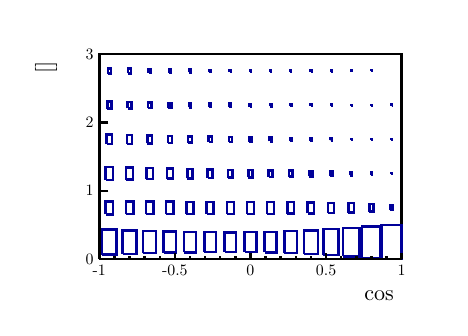
\begin{tikzpicture}
\pgfdeclareplotmark{cross} {
\pgfpathmoveto{\pgfpoint{-0.3\pgfplotmarksize}{\pgfplotmarksize}}
\pgfpathlineto{\pgfpoint{+0.3\pgfplotmarksize}{\pgfplotmarksize}}
\pgfpathlineto{\pgfpoint{+0.3\pgfplotmarksize}{0.3\pgfplotmarksize}}
\pgfpathlineto{\pgfpoint{+1\pgfplotmarksize}{0.3\pgfplotmarksize}}
\pgfpathlineto{\pgfpoint{+1\pgfplotmarksize}{-0.3\pgfplotmarksize}}
\pgfpathlineto{\pgfpoint{+0.3\pgfplotmarksize}{-0.3\pgfplotmarksize}}
\pgfpathlineto{\pgfpoint{+0.3\pgfplotmarksize}{-1.\pgfplotmarksize}}
\pgfpathlineto{\pgfpoint{-0.3\pgfplotmarksize}{-1.\pgfplotmarksize}}
\pgfpathlineto{\pgfpoint{-0.3\pgfplotmarksize}{-0.3\pgfplotmarksize}}
\pgfpathlineto{\pgfpoint{-1.\pgfplotmarksize}{-0.3\pgfplotmarksize}}
\pgfpathlineto{\pgfpoint{-1.\pgfplotmarksize}{0.3\pgfplotmarksize}}
\pgfpathlineto{\pgfpoint{-0.3\pgfplotmarksize}{0.3\pgfplotmarksize}}
\pgfpathclose
\pgfusepathqstroke
}
\pgfdeclareplotmark{cross*} {
\pgfpathmoveto{\pgfpoint{-0.3\pgfplotmarksize}{\pgfplotmarksize}}
\pgfpathlineto{\pgfpoint{+0.3\pgfplotmarksize}{\pgfplotmarksize}}
\pgfpathlineto{\pgfpoint{+0.3\pgfplotmarksize}{0.3\pgfplotmarksize}}
\pgfpathlineto{\pgfpoint{+1\pgfplotmarksize}{0.3\pgfplotmarksize}}
\pgfpathlineto{\pgfpoint{+1\pgfplotmarksize}{-0.3\pgfplotmarksize}}
\pgfpathlineto{\pgfpoint{+0.3\pgfplotmarksize}{-0.3\pgfplotmarksize}}
\pgfpathlineto{\pgfpoint{+0.3\pgfplotmarksize}{-1.\pgfplotmarksize}}
\pgfpathlineto{\pgfpoint{-0.3\pgfplotmarksize}{-1.\pgfplotmarksize}}
\pgfpathlineto{\pgfpoint{-0.3\pgfplotmarksize}{-0.3\pgfplotmarksize}}
\pgfpathlineto{\pgfpoint{-1.\pgfplotmarksize}{-0.3\pgfplotmarksize}}
\pgfpathlineto{\pgfpoint{-1.\pgfplotmarksize}{0.3\pgfplotmarksize}}
\pgfpathlineto{\pgfpoint{-0.3\pgfplotmarksize}{0.3\pgfplotmarksize}}
\pgfpathclose
\pgfusepathqfillstroke
}
\pgfdeclareplotmark{newstar} {
\pgfpathmoveto{\pgfqpoint{0pt}{\pgfplotmarksize}}
\pgfpathlineto{\pgfqpointpolar{44}{0.5\pgfplotmarksize}}
\pgfpathlineto{\pgfqpointpolar{18}{\pgfplotmarksize}}
\pgfpathlineto{\pgfqpointpolar{-20}{0.5\pgfplotmarksize}}
\pgfpathlineto{\pgfqpointpolar{-54}{\pgfplotmarksize}}
\pgfpathlineto{\pgfqpointpolar{-90}{0.5\pgfplotmarksize}}
\pgfpathlineto{\pgfqpointpolar{234}{\pgfplotmarksize}}
\pgfpathlineto{\pgfqpointpolar{198}{0.5\pgfplotmarksize}}
\pgfpathlineto{\pgfqpointpolar{162}{\pgfplotmarksize}}
\pgfpathlineto{\pgfqpointpolar{134}{0.5\pgfplotmarksize}}
\pgfpathclose
\pgfusepathqstroke
}
\pgfdeclareplotmark{newstar*} {
\pgfpathmoveto{\pgfqpoint{0pt}{\pgfplotmarksize}}
\pgfpathlineto{\pgfqpointpolar{44}{0.5\pgfplotmarksize}}
\pgfpathlineto{\pgfqpointpolar{18}{\pgfplotmarksize}}
\pgfpathlineto{\pgfqpointpolar{-20}{0.5\pgfplotmarksize}}
\pgfpathlineto{\pgfqpointpolar{-54}{\pgfplotmarksize}}
\pgfpathlineto{\pgfqpointpolar{-90}{0.5\pgfplotmarksize}}
\pgfpathlineto{\pgfqpointpolar{234}{\pgfplotmarksize}}
\pgfpathlineto{\pgfqpointpolar{198}{0.5\pgfplotmarksize}}
\pgfpathlineto{\pgfqpointpolar{162}{\pgfplotmarksize}}
\pgfpathlineto{\pgfqpointpolar{134}{0.5\pgfplotmarksize}}
\pgfpathclose
\pgfusepathqfillstroke
}
\definecolor{c}{rgb}{1,1,1};
\draw [color=c, fill=c] (5.1,3.46332) rectangle (9.9,6.72292);
\draw [color=c, fill=c] (5.58,3.78928) rectangle (9.42,6.39696);
\definecolor{c}{rgb}{0,0,0};
\draw [c,line width=0.9] (5.58,3.78928) -- (5.58,6.39696) -- (9.42,6.39696) -- (9.42,3.78928) -- (5.58,3.78928);
\definecolor{c}{rgb}{1,1,1};
\draw [color=c, fill=c] (5.58,3.78928) rectangle (9.42,6.39696);
\definecolor{c}{rgb}{0,0,0};
\draw [c,line width=0.9] (5.58,3.78928) -- (5.58,6.39696) -- (9.42,6.39696) -- (9.42,3.78928) -- (5.58,3.78928);
\definecolor{c}{rgb}{0,0,0.6};
\draw [c,line width=0.9] (5.6146,3.84803) -- (5.6146,4.16515) -- (5.8014,4.16515) -- (5.8014,3.84803) -- (5.6146,3.84803);
\draw [c,line width=0.9] (5.87575,3.85677) -- (5.87575,4.15641) -- (6.05225,4.15641) -- (6.05225,3.85677) -- (5.87575,3.85677);
\draw [c,line width=0.9] (6.13731,3.8662) -- (6.13731,4.14698) -- (6.30269,4.14698) -- (6.30269,3.8662) -- (6.13731,3.8662);
\draw [c,line width=0.9] (6.39701,3.87249) -- (6.39701,4.14069) -- (6.55499,4.14069) -- (6.55499,3.87249) -- (6.39701,3.87249);
\draw [c,line width=0.9] (6.65598,3.87753) -- (6.65598,4.13565) -- (6.80802,4.13565) -- (6.80802,3.87753) -- (6.65598,3.87753);
\draw [c,line width=0.9] (6.91419,3.88128) -- (6.91419,4.1319) -- (7.06181,4.1319) -- (7.06181,3.88128) -- (6.91419,3.88128);
\draw [c,line width=0.9] (7.17088,3.88246) -- (7.17088,4.13072) -- (7.31712,4.13072) -- (7.31712,3.88246) -- (7.17088,3.88246);
\draw [c,line width=0.9] (7.42583,3.88068) -- (7.42583,4.1325) -- (7.57417,4.1325) -- (7.57417,3.88068) -- (7.42583,3.88068);
\draw [c,line width=0.9] (7.67923,3.87627) -- (7.67923,4.13692) -- (7.83277,4.13692) -- (7.83277,3.87627) -- (7.67923,3.87627);
\draw [c,line width=0.9] (7.93036,3.86799) -- (7.93036,4.14519) -- (8.09364,4.14519) -- (8.09364,3.86799) -- (7.93036,3.86799);
\draw [c,line width=0.9] (8.17978,3.85683) -- (8.17978,4.15635) -- (8.35622,4.15635) -- (8.35622,3.85683) -- (8.17978,3.85683);
\draw [c,line width=0.9] (8.42754,3.84283) -- (8.42754,4.17035) -- (8.62046,4.17035) -- (8.62046,3.84283) -- (8.42754,3.84283);
\draw [c,line width=0.9] (8.67353,3.82584) -- (8.67353,4.18734) -- (8.88647,4.18734) -- (8.88647,3.82584) -- (8.67353,3.82584);
\draw [c,line width=0.9] (8.91885,3.8077) -- (8.91885,4.20548) -- (9.15315,4.20548) -- (9.15315,3.8077) -- (8.91885,3.8077);
\draw [c,line width=0.9] (9.164,3.78928) -- (9.164,4.2239) -- (9.42,4.2239) -- (9.42,3.78928) -- (9.164,3.78928);
\draw [c,line width=0.9] (5.66003,4.35977) -- (5.66003,4.52264) -- (5.75597,4.52264) -- (5.75597,4.35977) -- (5.66003,4.35977);
\draw [c,line width=0.9] (5.91643,4.36045) -- (5.91643,4.52196) -- (6.01157,4.52196) -- (6.01157,4.36045) -- (5.91643,4.36045);
\draw [c,line width=0.9] (6.17284,4.36113) -- (6.17284,4.52128) -- (6.26716,4.52128) -- (6.26716,4.36113) -- (6.17284,4.36113);
\draw [c,line width=0.9] (6.42953,4.36232) -- (6.42953,4.52009) -- (6.52247,4.52009) -- (6.52247,4.36232) -- (6.42953,4.36232);
\draw [c,line width=0.9] (6.68665,4.3642) -- (6.68665,4.5182) -- (6.77735,4.5182) -- (6.77735,4.3642) -- (6.68665,4.3642);
\draw [c,line width=0.9] (6.94316,4.36508) -- (6.94316,4.51733) -- (7.03284,4.51733) -- (7.03284,4.36508) -- (6.94316,4.36508);
\draw [c,line width=0.9] (7.19962,4.36586) -- (7.19962,4.51654) -- (7.28838,4.51654) -- (7.28838,4.36586) -- (7.19962,4.36586);
\draw [c,line width=0.9] (7.45581,4.36618) -- (7.45581,4.51623) -- (7.54419,4.51623) -- (7.54419,4.36618) -- (7.45581,4.36618);
\draw [c,line width=0.9] (7.71199,4.36648) -- (7.71199,4.51593) -- (7.80001,4.51593) -- (7.80001,4.36648) -- (7.71199,4.36648);
\draw [c,line width=0.9] (7.96874,4.36776) -- (7.96874,4.51465) -- (8.05526,4.51465) -- (8.05526,4.36776) -- (7.96874,4.36776);
\draw [c,line width=0.9] (8.2265,4.37075) -- (8.2265,4.51165) -- (8.3095,4.51165) -- (8.3095,4.37075) -- (8.2265,4.37075);
\draw [c,line width=0.9] (8.48563,4.37607) -- (8.48563,4.50634) -- (8.56237,4.50634) -- (8.56237,4.37607) -- (8.48563,4.37607);
\draw [c,line width=0.9] (8.74475,4.38136) -- (8.74475,4.50105) -- (8.81525,4.50105) -- (8.81525,4.38136) -- (8.74475,4.38136);
\draw [c,line width=0.9] (9.00873,4.39491) -- (9.00873,4.4875) -- (9.06327,4.4875) -- (9.06327,4.39491) -- (9.00873,4.39491);
\draw [c,line width=0.9] (9.27598,4.41401) -- (9.27598,4.4684) -- (9.30802,4.4684) -- (9.30802,4.41401) -- (9.27598,4.41401);
\draw [c,line width=0.9] (5.65948,4.79344) -- (5.65948,4.95819) -- (5.75652,4.95819) -- (5.75652,4.79344) -- (5.65948,4.79344);
\draw [c,line width=0.9] (5.91885,4.79917) -- (5.91885,4.95247) -- (6.00915,4.95247) -- (6.00915,4.79917) -- (5.91885,4.79917);
\draw [c,line width=0.9] (6.17889,4.80603) -- (6.17889,4.94561) -- (6.26111,4.94561) -- (6.26111,4.80603) -- (6.17889,4.80603);
\draw [c,line width=0.9] (6.43829,4.81179) -- (6.43829,4.93984) -- (6.51371,4.93984) -- (6.51371,4.81179) -- (6.43829,4.81179);
\draw [c,line width=0.9] (6.69762,4.81745) -- (6.69762,4.93419) -- (6.76638,4.93419) -- (6.76638,4.81745) -- (6.69762,4.81745);
\draw [c,line width=0.9] (6.95684,4.82292) -- (6.95684,4.92871) -- (7.01916,4.92871) -- (7.01916,4.82292) -- (6.95684,4.82292);
\draw [c,line width=0.9] (7.21527,4.82704) -- (7.21527,4.9246) -- (7.27273,4.9246) -- (7.27273,4.82704) -- (7.21527,4.82704);
\draw [c,line width=0.9] (7.47306,4.83007) -- (7.47306,4.92156) -- (7.52694,4.92156) -- (7.52694,4.83007) -- (7.47306,4.83007);
\draw [c,line width=0.9] (7.73081,4.83306) -- (7.73081,4.91858) -- (7.78119,4.91858) -- (7.78119,4.83306) -- (7.73081,4.83306);
\draw [c,line width=0.9] (7.98948,4.83759) -- (7.98948,4.91405) -- (8.03452,4.91405) -- (8.03452,4.83759) -- (7.98948,4.83759);
\draw [c,line width=0.9] (8.24832,4.84241) -- (8.24832,4.90922) -- (8.28768,4.90922) -- (8.28768,4.84241) -- (8.24832,4.84241);
\draw [c,line width=0.9] (8.50784,4.84837) -- (8.50784,4.90326) -- (8.54016,4.90326) -- (8.54016,4.84837) -- (8.50784,4.84837);
\draw [c,line width=0.9] (8.76773,4.85498) -- (8.76773,4.89665) -- (8.79227,4.89665) -- (8.79227,4.85498) -- (8.76773,4.85498);
\draw [c,line width=0.9] (9.02777,4.86185) -- (9.02777,4.88979) -- (9.04423,4.88979) -- (9.04423,4.86185) -- (9.02777,4.86185);
\draw [c,line width=0.9] (9.28822,4.8694) -- (9.28822,4.88223) -- (9.29578,4.88223) -- (9.29578,4.8694) -- (9.28822,4.8694);
\draw [c,line width=0.9] (5.67229,5.2498) -- (5.67229,5.37106) -- (5.74371,5.37106) -- (5.74371,5.2498) -- (5.67229,5.2498);
\draw [c,line width=0.9] (5.93165,5.2555) -- (5.93165,5.36536) -- (5.99635,5.36536) -- (5.99635,5.2555) -- (5.93165,5.2555);
\draw [c,line width=0.9] (6.19091,5.26105) -- (6.19091,5.35981) -- (6.24909,5.35981) -- (6.24909,5.26105) -- (6.19091,5.26105);
\draw [c,line width=0.9] (6.44996,5.26622) -- (6.44996,5.35464) -- (6.50204,5.35464) -- (6.50204,5.26622) -- (6.44996,5.26622);
\draw [c,line width=0.9] (6.70837,5.27032) -- (6.70837,5.35054) -- (6.75563,5.35054) -- (6.75563,5.27032) -- (6.70837,5.27032);
\draw [c,line width=0.9] (6.96737,5.2754) -- (6.96737,5.34546) -- (7.00863,5.34546) -- (7.00863,5.2754) -- (6.96737,5.2754);
\draw [c,line width=0.9] (7.22567,5.2793) -- (7.22567,5.34156) -- (7.26233,5.34156) -- (7.26233,5.2793) -- (7.22567,5.2793);
\draw [c,line width=0.9] (7.48373,5.2828) -- (7.48373,5.33806) -- (7.51627,5.33806) -- (7.51627,5.2828) -- (7.48373,5.2828);
\draw [c,line width=0.9] (7.74231,5.28718) -- (7.74231,5.33368) -- (7.76969,5.33368) -- (7.76969,5.28718) -- (7.74231,5.28718);
\draw [c,line width=0.9] (8,5.29006) -- (8,5.3308) -- (8.024,5.3308) -- (8.024,5.29006) -- (8,5.29006);
\draw [c,line width=0.9] (8.25805,5.29353) -- (8.25805,5.32733) -- (8.27795,5.32733) -- (8.27795,5.29353) -- (8.25805,5.29353);
\draw [c,line width=0.9] (8.51663,5.29792) -- (8.51663,5.32294) -- (8.53137,5.32294) -- (8.53137,5.29792) -- (8.51663,5.29792);
\draw [c,line width=0.9] (8.77491,5.30178) -- (8.77491,5.31908) -- (8.78509,5.31908) -- (8.78509,5.30178) -- (8.77491,5.30178);
\draw [c,line width=0.9] (9.03261,5.30468) -- (9.03261,5.31618) -- (9.03992,5.31618) -- (9.03992,5.30468) -- (9.03261,5.30468);
\draw [c,line width=0.9] (9.2905,5.30788) -- (9.2905,5.31518) -- (9.2978,5.31518) -- (9.2978,5.30788) -- (9.2905,5.30788);
\draw [c,line width=0.9] (5.68176,5.7005) -- (5.68176,5.78958) -- (5.73424,5.78958) -- (5.73424,5.7005) -- (5.68176,5.7005);
\draw [c,line width=0.9] (5.94049,5.70514) -- (5.94049,5.78495) -- (5.98751,5.78495) -- (5.98751,5.70514) -- (5.94049,5.70514);
\draw [c,line width=0.9] (6.19913,5.70961) -- (6.19913,5.78047) -- (6.24087,5.78047) -- (6.24087,5.70961) -- (6.19913,5.70961);
\draw [c,line width=0.9] (6.45771,5.71399) -- (6.45771,5.7761) -- (6.49429,5.7761) -- (6.49429,5.71399) -- (6.45771,5.71399);
\draw [c,line width=0.9] (6.71634,5.71846) -- (6.71634,5.77162) -- (6.74766,5.77162) -- (6.74766,5.71846) -- (6.71634,5.71846);
\draw [c,line width=0.9] (6.97476,5.72256) -- (6.97476,5.76752) -- (7.00124,5.76752) -- (7.00124,5.72256) -- (6.97476,5.72256);
\draw [c,line width=0.9] (7.2323,5.72517) -- (7.2323,5.76491) -- (7.2557,5.76491) -- (7.2557,5.72517) -- (7.2323,5.72517);
\draw [c,line width=0.9] (7.49002,5.7281) -- (7.49002,5.76198) -- (7.50998,5.76198) -- (7.50998,5.7281) -- (7.49002,5.7281);
\draw [c,line width=0.9] (7.74782,5.73116) -- (7.74782,5.75892) -- (7.76418,5.75892) -- (7.76418,5.73116) -- (7.74782,5.73116);
\draw [c,line width=0.9] (8.00543,5.73389) -- (8.00543,5.7562) -- (8.01857,5.7562) -- (8.01857,5.73389) -- (8.00543,5.73389);
\draw [c,line width=0.9] (8.26279,5.7362) -- (8.26279,5.75389) -- (8.27321,5.75389) -- (8.27321,5.7362) -- (8.26279,5.7362);
\draw [c,line width=0.9] (8.52009,5.7384) -- (8.52009,5.75169) -- (8.52791,5.75169) -- (8.52791,5.7384) -- (8.52009,5.7384);
\draw [c,line width=0.9] (8.7775,5.74079) -- (8.7775,5.74929) -- (8.7848,5.74929) -- (8.7848,5.74079) -- (8.7775,5.74079);
\draw [c,line width=0.9] (9.03438,5.7423) -- (9.03438,5.74961) -- (9.04169,5.74961) -- (9.04169,5.7423) -- (9.03438,5.7423);
\draw [c,line width=0.9] (9.29158,5.74433) -- (9.29158,5.75164) -- (9.29889,5.75164) -- (9.29889,5.74433) -- (9.29158,5.74433);
\draw [c,line width=0.9] (5.68796,6.14563) -- (5.68796,6.21369) -- (5.72804,6.21369) -- (5.72804,6.14563) -- (5.68796,6.14563);
\draw [c,line width=0.9] (5.94661,6.15013) -- (5.94661,6.20919) -- (5.98139,6.20919) -- (5.98139,6.15013) -- (5.94661,6.15013);
\draw [c,line width=0.9] (6.20544,6.15493) -- (6.20544,6.20438) -- (6.23456,6.20438) -- (6.23456,6.15493) -- (6.20544,6.15493);
\draw [c,line width=0.9] (6.46347,6.15838) -- (6.46347,6.20093) -- (6.48853,6.20093) -- (6.48853,6.15838) -- (6.46347,6.15838);
\draw [c,line width=0.9] (6.7215,6.16183) -- (6.7215,6.19748) -- (6.7425,6.19748) -- (6.7425,6.16183) -- (6.7215,6.16183);
\draw [c,line width=0.9] (6.97915,6.16463) -- (6.97915,6.19468) -- (6.99685,6.19468) -- (6.99685,6.16463) -- (6.97915,6.16463);
\draw [c,line width=0.9] (7.23682,6.16747) -- (7.23682,6.19184) -- (7.25118,6.19184) -- (7.25118,6.16747) -- (7.23682,6.16747);
\draw [c,line width=0.9] (7.49366,6.16889) -- (7.49366,6.19042) -- (7.50634,6.19042) -- (7.50634,6.16889) -- (7.49366,6.16889);
\draw [c,line width=0.9] (7.75082,6.17087) -- (7.75082,6.18845) -- (7.76118,6.18845) -- (7.76118,6.17087) -- (7.75082,6.17087);
\draw [c,line width=0.9] (8.00779,6.1725) -- (8.00779,6.18681) -- (8.01621,6.18681) -- (8.01621,6.1725) -- (8.00779,6.1725);
\draw [c,line width=0.9] (8.26485,6.17431) -- (8.26485,6.185) -- (8.27216,6.185) -- (8.27216,6.17431) -- (8.26485,6.17431);
\draw [c,line width=0.9] (8.52183,6.17598) -- (8.52183,6.18334) -- (8.52914,6.18334) -- (8.52914,6.17598) -- (8.52183,6.17598);
\draw [c,line width=0.9] (8.7785,6.1771) -- (8.7785,6.18441) -- (8.7858,6.18441) -- (8.7858,6.1771) -- (8.7785,6.1771);
\draw [c,line width=0.9] (9.03541,6.17865) -- (9.03541,6.18596) -- (9.04272,6.18596) -- (9.04272,6.17865) -- (9.03541,6.17865);
\definecolor{c}{rgb}{0,0,0};
\draw [c,line width=0.9] (5.58,3.78928) -- (9.42,3.78928);
\draw [anchor= east] (9.42,3.33033) node[scale=0.797299, color=c, rotate=0]{$\cos\thetaK$};
\draw [c,line width=0.9] (5.58,3.86751) -- (5.58,3.78928);
\draw [c,line width=0.9] (5.772,3.8284) -- (5.772,3.78928);
\draw [c,line width=0.9] (5.964,3.8284) -- (5.964,3.78928);
\draw [c,line width=0.9] (6.156,3.8284) -- (6.156,3.78928);
\draw [c,line width=0.9] (6.348,3.8284) -- (6.348,3.78928);
\draw [c,line width=0.9] (6.54,3.86751) -- (6.54,3.78928);
\draw [c,line width=0.9] (6.732,3.8284) -- (6.732,3.78928);
\draw [c,line width=0.9] (6.924,3.8284) -- (6.924,3.78928);
\draw [c,line width=0.9] (7.116,3.8284) -- (7.116,3.78928);
\draw [c,line width=0.9] (7.308,3.8284) -- (7.308,3.78928);
\draw [c,line width=0.9] (7.5,3.86751) -- (7.5,3.78928);
\draw [c,line width=0.9] (7.692,3.8284) -- (7.692,3.78928);
\draw [c,line width=0.9] (7.884,3.8284) -- (7.884,3.78928);
\draw [c,line width=0.9] (8.076,3.8284) -- (8.076,3.78928);
\draw [c,line width=0.9] (8.268,3.8284) -- (8.268,3.78928);
\draw [c,line width=0.9] (8.46,3.86751) -- (8.46,3.78928);
\draw [c,line width=0.9] (8.652,3.8284) -- (8.652,3.78928);
\draw [c,line width=0.9] (8.844,3.8284) -- (8.844,3.78928);
\draw [c,line width=0.9] (9.036,3.8284) -- (9.036,3.78928);
\draw [c,line width=0.9] (9.228,3.8284) -- (9.228,3.78928);
\draw [c,line width=0.9] (9.42,3.86751) -- (9.42,3.78928);
\draw [anchor=base] (5.58,3.58067) node[scale=0.574055, color=c, rotate=0]{-1};
\draw [anchor=base] (6.54,3.58067) node[scale=0.574055, color=c, rotate=0]{-0.5};
\draw [anchor=base] (7.5,3.58067) node[scale=0.574055, color=c, rotate=0]{0};
\draw [anchor=base] (8.46,3.58067) node[scale=0.574055, color=c, rotate=0]{0.5};
\draw [anchor=base] (9.42,3.58067) node[scale=0.574055, color=c, rotate=0]{1};
\draw [c,line width=0.9] (5.58,3.78928) -- (5.58,6.39696);
\draw [anchor= east] (4.90416,6.39696) node[scale=0.797299, color=c, rotate=90]{$\ptrans{\pion} [\mevcc]$};
\draw [c,line width=0.9] (5.6952,3.78928) -- (5.58,3.78928);
\draw [c,line width=0.9] (5.6952,4.65851) -- (5.58,4.65851);
\draw [c,line width=0.9] (5.6952,5.52774) -- (5.58,5.52774);
\draw [c,line width=0.9] (5.6952,6.39696) -- (5.58,6.39696);
\draw [anchor= east] (5.58,3.78928) node[scale=0.574055, color=c, rotate=0]{0};
\draw [anchor= east] (5.58,4.65851) node[scale=0.574055, color=c, rotate=0]{1};
\draw [anchor= east] (5.58,5.52774) node[scale=0.574055, color=c, rotate=0]{2};
\draw [anchor= east] (5.58,6.39696) node[scale=0.574055, color=c, rotate=0]{3};
\end{tikzpicture}
}
    \caption{}
    \label{ctk_pion_pt}
  \end{subfigure}
  \caption{Two dimensional histograms of kaon (left) and pion (right) transverse momentum in the lab frame versus $\cos\thetaK$.
           No detector effects and no selection are included. The area of the boxes reflect the number of bin entries.}
  \label{ctk_hadrons_pt}
\end{figure}

\noindent where, $\thetapi^\lab$ is the angle of the pion momentum vector with respect to the boost direction
in the lab frame. Absence of the \lab superscript refers to quantities computed in the \Kstarz rest frame.
The subscripts T,L label the transverse and longitudinal components of the pion momentum, $\ptot_{\pi}$.
The symbol $E$ stands for the energy of the pions. The Lorentz boost factor and the relativistic speed
are labeled by $\gamma$ and $\beta$ respectively. The angle $\thetapi$ is the angle of the pion momentum,
in the \Kstarz rest frame, which is related to $\thetaK$ in \figref{helAngles} as: $\thetapi = \thetaK + \pi$.
Now, the origin of the above-mentioned asymmetry is understood better in the limit of a massless pion,
in which case \equref{pi_angle} reduces to:

\begin{equation}
  \centering
  \tan\thetapi^\lab = \frac{\sin\thetapi}{\gamma\parenthesis{\cos\thetapi + 1} }.
  \label{pi_angle_massless}
\end{equation}

\noindent Note that the energy of a massless particle is equal to its total momentum and also that $\beta \simeq 1$
for pions coming from \BJpsiKpi decays in \lhcb. From \equref{pi_angle_massless} it follows that decays where $\cos\thetapi=-1$
are not allowed. The situation corresponds to a low transverse momentum pion for which $\cos\thetaK = -\cos\thetapi = +1$.
This explains why the shape of the $\cos\thetaK$ distribution becomes asymmetric when excluding low momenta pions.
This effect is more general and it is driven by the mass difference between the two particles in a two body decay.

Coming now to the case of the $\cos\thetamu$ acceptance shape, the two decay products of the \jpsi have
the same mass and thus get the same momentum fraction out of the mother \jpsi particle. A consequence of
the latter is that the transverse momentum spectrum of the two muons is identical, excluding detector
resolution, and thus the two muons populate the $(\pt-\cos\thetamu)$ plane similarly. Based on the latter
it follows that excluding low transverse momentum muons does not introduce any asymmetry in the $\cos\thetamu$ distribution.

As for the acceptance in the $\phihel$ plane it is very close to being uniform.
No strong acceptance effect in that projection is expected.

\subsubsection{Acceptance parametrization}
\label{Acceptance parametrization}
As for the parametrization of the angular acceptance, there are at least two ways to proceed,
namely the \emph{efficiency moments} \cite{jeroenThesis} and the \emph{normalization weights} \cite{tristanThesis,jeroenThesis}.
The current analysis implements the first one. The efficiency function is thus parameterized using orthogonal polynomials,
which, when combined with the angular description formalism in the previous subsection, allows for fast analytic
integration. Such a parametrization is:

\begin{equation}
  \centering
  \epsilon(\Omega) = \sum_{ijk} \; \moment{i}{j}{k} \; P_i^0(\cos\thetaK) \; Y_{jk}(\cos\thetamu,\phihel) \equiv \moment{i}{j}{k} \; \effbase,
  \label{eff_func}
\end{equation}

\noindent where the real-valued spherical harmonics ($Y$) and associated Legendre polynomials ($P$) are used as the basis
functions to which the angular acceptance is decomposed by means of the coefficients $c^i_{k}$, hereafter efficiency moments or simply moments.
Following the parametrization of \equref{eff_func} one just needs to obtain a set of $c^i_{jk}$. Note that there are \aprior infinite efficiency moments
since the sum in \equref{eff_func} runs through all possible values of the $ijk$ indices. However, in practice only a small number of efficiency moments
contribute significantly to the angular acceptance shape. This is due to the fact that higher moments introduce
variations on the acceptance shape that are effectively washed out by the finite angular resolution.

The efficiency moments used to describe the acceptance shape are shown in the first column of \tabref{eff_moms_table}.
The larger the value of a moment, the more the corresponding function contributes to the overall efficiency function.
The efficiency functions $P_1^0Y_{00}$ and $P_2^0Y_{00}$ account for most of the hard acceptance drop in the $\cos\thetaK$ projection.
This is supported by the large value of the corresponding moments $\moment{1}{0}{0}$ and $\moment{2}{0}{0}$.
The choice of the particular efficiency moments, is connected to an important
issue with the acceptance structure close to $\cos\thetaK=1$ and it is addressed at the end of the current section.

\begin{table}[!t]
  \centering
  \renewcommand{\arraystretch}{1.2}
  \begin{tabular}{ccc}
    \hline
    moment & central value & standard deviation \\
    \hline
  $\moment{0}{0}{0}$   & $+3.7454$  &  $0.0023$  \\
  $\moment{1}{0}{0}$   & $-2.0982$  &  $0.0084$  \\
  $\moment{2}{0}{0}$   & $-1.9116$  &  $0.0126$  \\
  $\moment{3}{0}{0}$   & $-0.0317$  &  $0.0151$  \\
  $\moment{4}{0}{0}$   & $+0.1146$  &  $0.0175$  \\
  $\moment{5}{0}{0}$   & $+0.1384$  &  $0.0193$  \\
  $\moment{0}{2}{0}$   & $+0.2820$  &  $0.0066$  \\
  $\moment{0}{2}{2}$   & $+0.0612$  &  $0.0058$  \\
  $\moment{0}{4}{0}$   & $+0.0864$  &  $0.0066$  \\
  $\moment{1}{2}{0}$   & $-0.1900$  &  $0.0115$  \\
  $\moment{1}{4}{0}$   & $-0.0720$  &  $0.0118$  \\
  $\moment{2}{2}{0}$   & $-0.1315$  &  $0.0161$  \\
  $\moment{2}{2}{2}$   & $-0.0674$  &  $0.0117$  \\
  \hline
  \end{tabular}
  \caption{Efficiency moments of \BsJpsiKst.}
   \label{eff_moms_table}
\end{table}

In order for the efficiency moments $c^i_{jk}$ to be computed a definition of the efficiency is necessary. Note that this computation relies on
simulated data where all the generating conditions are known. The efficiency is defined as the ratio of two angular \pdfs, namely
\Pobs and \Pgen. The first is the angular \pdf that the simulated data follow after all stages of selection, whereas
the latter is the angular \pdf with which the simulated data has been generated.
It follows that the efficiency is defined as:

\begin{equation}
  \centering
  \Pobs = \epsilon(\Omega) \Pgen \quad \Rightarrow \quad \epsilon(\Omega) \equiv \frac{\Pobs}{\Pgen}.
  \label{eff_def}
\end{equation}

\noindent Computing the efficiency moments is done by projecting the efficiency as defined in \equref{eff_def}
on the orthogonal $PY$ basis. This projection is shown in the following equation:

\begin{align}
  \centering
   c^i_{jk}  \equiv & \parenthesis{j + \frac{1}{2}} \; \int \; d\Omega \; \effbase \; \epsilon(\Omega) \nonumber \\
                 =  & \parenthesis{j + \frac{1}{2}} \; \int \; d\Omega \; \Pobs \; \frac{\effbase}{\Pgen}.
  \label{eff_moms_def}
\end{align}

\noindent The factor $j+\frac{1}{2}$ is used to make it such that the associated Legendre polynomials form an
orthonormal basis; implying that the integral of the product of two associated Legendre polynomials is equal
to the {\it Kronecker delta} symbol. The later fact is required to properly normalize the efficiency moments.
The final step in the calculation of the efficiency moments is the computation of the integral in \equref{eff_moms_def}.
This is done by means of simulated data and the integral is computed following the concept of Monte Carlo integration. This implies
that the integral in \equref{eff_moms_def} can be estimated by a sum over the simulated data (which they have passed through the exact
same selection steps as data) as:

\begin{equation}
\centering
  E\left[ \int \; d\Omega \; \effbase \frac{\Pobs}{\Pgen} \right] = \frac{1}{\Nobs} \sum_e^{\Nobs} \frac{\effbase}{\Pgen}.
  \label{eff_moms_calc}
\end{equation}

\noindent Combining \equref{eff_moms_def} and \equref{eff_moms_calc} the final expression for computing the efficiency moments is shown
in \equref{eff_moms_calc_final} and the result of the computations can be found it table \tabref{eff_moms_table}

\begin{equation}
\centering
 c^i_{jk} \equiv (j + \frac{1}{2})  \frac{1}{\Nobs} \sum_e^{\Nobs} \frac{\effbase}{\Pgen}.
  \label{eff_moms_calc_final}
\end{equation}

\noindent Acceptance effects in the $\cos\thetamu$ projection are less pronounced compared to the one $\cos\thetaK$.
This can be deduced from \figref{angAcc_ctl} as well as from the values of moments like $\moment{0}{j}{k}$
compared to the values of $\moment{1}{0}{0}$ and $\moment{2}{0}{0}$. Lastly, the efficiency moments are
correlated and the corresponding correlation matrix can be found in \tabref{eff_moms_corr}.

\subsubsection{Choice of efficiency moments}
The choice of efficiency moments has to do with the structure of the acceptance at $\cos\thetaK=1$. At that point the acceptance goes to zero
which is not a problem by itself. However, within the parametrization of the acceptance function, \equref{eff_func} may become negative.
In other words the method of efficiency moments does not guarantee that the acceptance function is a positive definite quantity.
Note that this is an artifact of the parametrization. The problem is mathematical in nature and there is no standard solution (known
to the author when these lines were written). The approach followed to solve this problem has two steps: First a constraint on the
efficiency function, \equref{eff_func}, is introduced to force it to be positive definite and second, a fit to the efficiency
moments is performed to optimize the acceptance shape description. The result is a hybrid acceptance function that is by
construction positive definite.

Before laying out the formulas behind the above-mentioned steps it is useful to visualize the problem caused by the parametrization, see \figref{angAcc_nom}
and the corresponding caption. Subsequently, the most natural thing to do before making any effort to force the value of \equref{eff_func}
positive at $\cos\thetaK=1$ is to make the best possible choice of efficiency moments. The moments are chosen such that the efficiency function becomes negative
at the largest possible value of $\cos\thetaK$. In other words the crossing point of the red curve with the horizontal axis in \figref{angAcc_nom},
has to be as close to $\cos\thetaK=1$ as possible.

\begin{figure}[t]
  \centering
  \begin{subfigure}{0.5\textwidth}
    \raggedright
    \tikzsetnextfilename{eff_helcosthetaK_neg_all_raw_zoom}
    \scalebox{1.15}{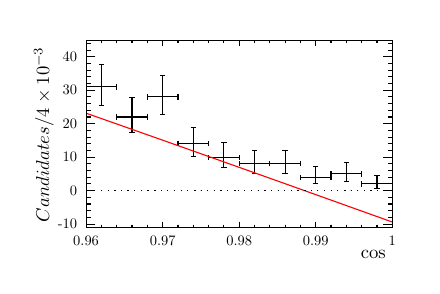
\begin{tikzpicture}
\pgfdeclareplotmark{cross} {
\pgfpathmoveto{\pgfpoint{-0.3\pgfplotmarksize}{\pgfplotmarksize}}
\pgfpathlineto{\pgfpoint{+0.3\pgfplotmarksize}{\pgfplotmarksize}}
\pgfpathlineto{\pgfpoint{+0.3\pgfplotmarksize}{0.3\pgfplotmarksize}}
\pgfpathlineto{\pgfpoint{+1\pgfplotmarksize}{0.3\pgfplotmarksize}}
\pgfpathlineto{\pgfpoint{+1\pgfplotmarksize}{-0.3\pgfplotmarksize}}
\pgfpathlineto{\pgfpoint{+0.3\pgfplotmarksize}{-0.3\pgfplotmarksize}}
\pgfpathlineto{\pgfpoint{+0.3\pgfplotmarksize}{-1.\pgfplotmarksize}}
\pgfpathlineto{\pgfpoint{-0.3\pgfplotmarksize}{-1.\pgfplotmarksize}}
\pgfpathlineto{\pgfpoint{-0.3\pgfplotmarksize}{-0.3\pgfplotmarksize}}
\pgfpathlineto{\pgfpoint{-1.\pgfplotmarksize}{-0.3\pgfplotmarksize}}
\pgfpathlineto{\pgfpoint{-1.\pgfplotmarksize}{0.3\pgfplotmarksize}}
\pgfpathlineto{\pgfpoint{-0.3\pgfplotmarksize}{0.3\pgfplotmarksize}}
\pgfpathclose
\pgfusepathqstroke
}
\pgfdeclareplotmark{cross*} {
\pgfpathmoveto{\pgfpoint{-0.3\pgfplotmarksize}{\pgfplotmarksize}}
\pgfpathlineto{\pgfpoint{+0.3\pgfplotmarksize}{\pgfplotmarksize}}
\pgfpathlineto{\pgfpoint{+0.3\pgfplotmarksize}{0.3\pgfplotmarksize}}
\pgfpathlineto{\pgfpoint{+1\pgfplotmarksize}{0.3\pgfplotmarksize}}
\pgfpathlineto{\pgfpoint{+1\pgfplotmarksize}{-0.3\pgfplotmarksize}}
\pgfpathlineto{\pgfpoint{+0.3\pgfplotmarksize}{-0.3\pgfplotmarksize}}
\pgfpathlineto{\pgfpoint{+0.3\pgfplotmarksize}{-1.\pgfplotmarksize}}
\pgfpathlineto{\pgfpoint{-0.3\pgfplotmarksize}{-1.\pgfplotmarksize}}
\pgfpathlineto{\pgfpoint{-0.3\pgfplotmarksize}{-0.3\pgfplotmarksize}}
\pgfpathlineto{\pgfpoint{-1.\pgfplotmarksize}{-0.3\pgfplotmarksize}}
\pgfpathlineto{\pgfpoint{-1.\pgfplotmarksize}{0.3\pgfplotmarksize}}
\pgfpathlineto{\pgfpoint{-0.3\pgfplotmarksize}{0.3\pgfplotmarksize}}
\pgfpathclose
\pgfusepathqfillstroke
}
\pgfdeclareplotmark{newstar} {
\pgfpathmoveto{\pgfqpoint{0pt}{\pgfplotmarksize}}
\pgfpathlineto{\pgfqpointpolar{44}{0.5\pgfplotmarksize}}
\pgfpathlineto{\pgfqpointpolar{18}{\pgfplotmarksize}}
\pgfpathlineto{\pgfqpointpolar{-20}{0.5\pgfplotmarksize}}
\pgfpathlineto{\pgfqpointpolar{-54}{\pgfplotmarksize}}
\pgfpathlineto{\pgfqpointpolar{-90}{0.5\pgfplotmarksize}}
\pgfpathlineto{\pgfqpointpolar{234}{\pgfplotmarksize}}
\pgfpathlineto{\pgfqpointpolar{198}{0.5\pgfplotmarksize}}
\pgfpathlineto{\pgfqpointpolar{162}{\pgfplotmarksize}}
\pgfpathlineto{\pgfqpointpolar{134}{0.5\pgfplotmarksize}}
\pgfpathclose
\pgfusepathqstroke
}
\pgfdeclareplotmark{newstar*} {
\pgfpathmoveto{\pgfqpoint{0pt}{\pgfplotmarksize}}
\pgfpathlineto{\pgfqpointpolar{44}{0.5\pgfplotmarksize}}
\pgfpathlineto{\pgfqpointpolar{18}{\pgfplotmarksize}}
\pgfpathlineto{\pgfqpointpolar{-20}{0.5\pgfplotmarksize}}
\pgfpathlineto{\pgfqpointpolar{-54}{\pgfplotmarksize}}
\pgfpathlineto{\pgfqpointpolar{-90}{0.5\pgfplotmarksize}}
\pgfpathlineto{\pgfqpointpolar{234}{\pgfplotmarksize}}
\pgfpathlineto{\pgfqpointpolar{198}{0.5\pgfplotmarksize}}
\pgfpathlineto{\pgfqpointpolar{162}{\pgfplotmarksize}}
\pgfpathlineto{\pgfqpointpolar{134}{0.5\pgfplotmarksize}}
\pgfpathclose
\pgfusepathqfillstroke
}
\definecolor{c}{rgb}{1,1,1};
\draw [color=c, fill=c] (0.1,3.20034) rectangle (4.9,6.21242);
\draw [color=c, fill=c] (0.772,3.68227) rectangle (4.66,6.06181);
\definecolor{c}{rgb}{0,0,0};
\draw [c] (0.772,3.68227) -- (0.772,6.06181) -- (4.66,6.06181) -- (4.66,3.68227) -- (0.772,3.68227);
\draw [c,line width=0.4] (0.772,3.68227) -- (4.66,3.68227);
\draw [anchor= east] (4.66,3.34492) node[scale=0.672711, rotate=0]{$\cos\thetaK$};
\draw [c,line width=0.4] (0.772,3.75546) -- (0.772,3.68227);
\draw [c,line width=0.4] (0.9664,3.71887) -- (0.9664,3.68227);
\draw [c,line width=0.4] (1.1608,3.71887) -- (1.1608,3.68227);
\draw [c,line width=0.4] (1.3552,3.71887) -- (1.3552,3.68227);
\draw [c,line width=0.4] (1.5496,3.71887) -- (1.5496,3.68227);
\draw [c,line width=0.4] (1.744,3.75546) -- (1.744,3.68227);
\draw [c,line width=0.4] (1.9384,3.71887) -- (1.9384,3.68227);
\draw [c,line width=0.4] (2.1328,3.71887) -- (2.1328,3.68227);
\draw [c,line width=0.4] (2.3272,3.71887) -- (2.3272,3.68227);
\draw [c,line width=0.4] (2.5216,3.71887) -- (2.5216,3.68227);
\draw [c,line width=0.4] (2.716,3.75546) -- (2.716,3.68227);
\draw [c,line width=0.4] (2.9104,3.71887) -- (2.9104,3.68227);
\draw [c,line width=0.4] (3.1048,3.71887) -- (3.1048,3.68227);
\draw [c,line width=0.4] (3.2992,3.71887) -- (3.2992,3.68227);
\draw [c,line width=0.4] (3.4936,3.71887) -- (3.4936,3.68227);
\draw [c,line width=0.4] (3.688,3.75546) -- (3.688,3.68227);
\draw [c,line width=0.4] (3.8824,3.71887) -- (3.8824,3.68227);
\draw [c,line width=0.4] (4.0768,3.71887) -- (4.0768,3.68227);
\draw [c,line width=0.4] (4.2712,3.71887) -- (4.2712,3.68227);
\draw [c,line width=0.4] (4.4656,3.71887) -- (4.4656,3.68227);
\draw [c,line width=0.4] (4.66,3.75546) -- (4.66,3.68227);
\draw [anchor=base] (0.772,3.45937) node[scale=0.52322, rotate=0]{0.96};
\draw [anchor=base] (1.744,3.45937) node[scale=0.52322, rotate=0]{0.97};
\draw [anchor=base] (2.716,3.45937) node[scale=0.52322, rotate=0]{0.98};
\draw [anchor=base] (3.688,3.45937) node[scale=0.52322, rotate=0]{0.99};
\draw [anchor=base] (4.66,3.45937) node[scale=0.52322, rotate=0]{1};
\draw [c,line width=0.4] (0.772,6.06181) -- (4.66,6.06181);
\draw [c,line width=0.4] (0.772,5.98862) -- (0.772,6.06181);
\draw [c,line width=0.4] (0.9664,6.02522) -- (0.9664,6.06181);
\draw [c,line width=0.4] (1.1608,6.02522) -- (1.1608,6.06181);
\draw [c,line width=0.4] (1.3552,6.02522) -- (1.3552,6.06181);
\draw [c,line width=0.4] (1.5496,6.02522) -- (1.5496,6.06181);
\draw [c,line width=0.4] (1.744,5.98862) -- (1.744,6.06181);
\draw [c,line width=0.4] (1.9384,6.02522) -- (1.9384,6.06181);
\draw [c,line width=0.4] (2.1328,6.02522) -- (2.1328,6.06181);
\draw [c,line width=0.4] (2.3272,6.02522) -- (2.3272,6.06181);
\draw [c,line width=0.4] (2.5216,6.02522) -- (2.5216,6.06181);
\draw [c,line width=0.4] (2.716,5.98862) -- (2.716,6.06181);
\draw [c,line width=0.4] (2.9104,6.02522) -- (2.9104,6.06181);
\draw [c,line width=0.4] (3.1048,6.02522) -- (3.1048,6.06181);
\draw [c,line width=0.4] (3.2992,6.02522) -- (3.2992,6.06181);
\draw [c,line width=0.4] (3.4936,6.02522) -- (3.4936,6.06181);
\draw [c,line width=0.4] (3.688,5.98862) -- (3.688,6.06181);
\draw [c,line width=0.4] (3.8824,6.02522) -- (3.8824,6.06181);
\draw [c,line width=0.4] (4.0768,6.02522) -- (4.0768,6.06181);
\draw [c,line width=0.4] (4.2712,6.02522) -- (4.2712,6.06181);
\draw [c,line width=0.4] (4.4656,6.02522) -- (4.4656,6.06181);
\draw [c,line width=0.4] (4.66,5.98862) -- (4.66,6.06181);
\draw [c,line width=0.4] (0.772,3.68227) -- (0.772,6.06181);
\draw [anchor= east] (0.2344,6.06181) node[scale=0.672711, rotate=90]{$\text{Candidates} / 4\times10^{-3}$};
\draw [c,line width=0.4] (0.88576,3.72536) -- (0.772,3.72536);
\draw [c,line width=0.4] (0.82888,3.81032) -- (0.772,3.81032);
\draw [c,line width=0.4] (0.82888,3.89528) -- (0.772,3.89528);
\draw [c,line width=0.4] (0.82888,3.98024) -- (0.772,3.98024);
\draw [c,line width=0.4] (0.82888,4.06521) -- (0.772,4.06521);
\draw [c,line width=0.4] (0.88576,4.15017) -- (0.772,4.15017);
\draw [c,line width=0.4] (0.82888,4.23513) -- (0.772,4.23513);
\draw [c,line width=0.4] (0.82888,4.32009) -- (0.772,4.32009);
\draw [c,line width=0.4] (0.82888,4.40505) -- (0.772,4.40505);
\draw [c,line width=0.4] (0.82888,4.49002) -- (0.772,4.49002);
\draw [c,line width=0.4] (0.88576,4.57498) -- (0.772,4.57498);
\draw [c,line width=0.4] (0.82888,4.65994) -- (0.772,4.65994);
\draw [c,line width=0.4] (0.82888,4.7449) -- (0.772,4.7449);
\draw [c,line width=0.4] (0.82888,4.82986) -- (0.772,4.82986);
\draw [c,line width=0.4] (0.82888,4.91482) -- (0.772,4.91482);
\draw [c,line width=0.4] (0.88576,4.99979) -- (0.772,4.99979);
\draw [c,line width=0.4] (0.82888,5.08475) -- (0.772,5.08475);
\draw [c,line width=0.4] (0.82888,5.16971) -- (0.772,5.16971);
\draw [c,line width=0.4] (0.82888,5.25467) -- (0.772,5.25467);
\draw [c,line width=0.4] (0.82888,5.33964) -- (0.772,5.33964);
\draw [c,line width=0.4] (0.88576,5.4246) -- (0.772,5.4246);
\draw [c,line width=0.4] (0.82888,5.50956) -- (0.772,5.50956);
\draw [c,line width=0.4] (0.82888,5.59452) -- (0.772,5.59452);
\draw [c,line width=0.4] (0.82888,5.67948) -- (0.772,5.67948);
\draw [c,line width=0.4] (0.82888,5.76445) -- (0.772,5.76445);
\draw [c,line width=0.4] (0.88576,5.84941) -- (0.772,5.84941);
\draw [c,line width=0.4] (0.88576,3.72536) -- (0.772,3.72536);
\draw [c,line width=0.4] (0.88576,5.84941) -- (0.772,5.84941);
\draw [c,line width=0.4] (0.82888,5.93437) -- (0.772,5.93437);
\draw [c,line width=0.4] (0.82888,6.01933) -- (0.772,6.01933);
\draw [anchor= east] (0.724,3.72536) node[scale=0.52322, rotate=0]{-10};
\draw [anchor= east] (0.724,4.15017) node[scale=0.52322, rotate=0]{0};
\draw [anchor= east] (0.724,4.57498) node[scale=0.52322, rotate=0]{10};
\draw [anchor= east] (0.724,4.99979) node[scale=0.52322, rotate=0]{20};
\draw [anchor= east] (0.724,5.4246) node[scale=0.52322, rotate=0]{30};
\draw [anchor= east] (0.724,5.84941) node[scale=0.52322, rotate=0]{40};
\draw [c,line width=0.4] (4.66,3.68227) -- (4.66,6.06181);
\draw [c,line width=0.4] (4.54624,3.72536) -- (4.66,3.72536);
\draw [c,line width=0.4] (4.60312,3.81032) -- (4.66,3.81032);
\draw [c,line width=0.4] (4.60312,3.89528) -- (4.66,3.89528);
\draw [c,line width=0.4] (4.60312,3.98024) -- (4.66,3.98024);
\draw [c,line width=0.4] (4.60312,4.06521) -- (4.66,4.06521);
\draw [c,line width=0.4] (4.54624,4.15017) -- (4.66,4.15017);
\draw [c,line width=0.4] (4.60312,4.23513) -- (4.66,4.23513);
\draw [c,line width=0.4] (4.60312,4.32009) -- (4.66,4.32009);
\draw [c,line width=0.4] (4.60312,4.40505) -- (4.66,4.40505);
\draw [c,line width=0.4] (4.60312,4.49002) -- (4.66,4.49002);
\draw [c,line width=0.4] (4.54624,4.57498) -- (4.66,4.57498);
\draw [c,line width=0.4] (4.60312,4.65994) -- (4.66,4.65994);
\draw [c,line width=0.4] (4.60312,4.7449) -- (4.66,4.7449);
\draw [c,line width=0.4] (4.60312,4.82986) -- (4.66,4.82986);
\draw [c,line width=0.4] (4.60312,4.91482) -- (4.66,4.91482);
\draw [c,line width=0.4] (4.54624,4.99979) -- (4.66,4.99979);
\draw [c,line width=0.4] (4.60312,5.08475) -- (4.66,5.08475);
\draw [c,line width=0.4] (4.60312,5.16971) -- (4.66,5.16971);
\draw [c,line width=0.4] (4.60312,5.25467) -- (4.66,5.25467);
\draw [c,line width=0.4] (4.60312,5.33964) -- (4.66,5.33964);
\draw [c,line width=0.4] (4.54624,5.4246) -- (4.66,5.4246);
\draw [c,line width=0.4] (4.60312,5.50956) -- (4.66,5.50956);
\draw [c,line width=0.4] (4.60312,5.59452) -- (4.66,5.59452);
\draw [c,line width=0.4] (4.60312,5.67948) -- (4.66,5.67948);
\draw [c,line width=0.4] (4.60312,5.76445) -- (4.66,5.76445);
\draw [c,line width=0.4] (4.54624,5.84941) -- (4.66,5.84941);
\draw [c,line width=0.4] (4.54624,3.72536) -- (4.66,3.72536);
\draw [c,line width=0.4] (4.54624,5.84941) -- (4.66,5.84941);
\draw [c,line width=0.4] (4.60312,5.93437) -- (4.66,5.93437);
\draw [c,line width=0.4] (4.60312,6.01933) -- (4.66,6.01933);
\draw [c,line width=0.4] (0.9664,5.46708) -- (0.772,5.46708);
\draw [c,line width=0.4] (0.772,5.43352) -- (0.772,5.50064);
\draw [c,line width=0.4] (0.9664,5.46708) -- (1.1608,5.46708);
\draw [c,line width=0.4] (1.1608,5.43352) -- (1.1608,5.50064);
\draw [c,line width=0.4] (0.9664,5.46708) -- (0.9664,5.74863);
\draw [c,line width=0.4] (0.932843,5.74863) -- (0.999957,5.74863);
\draw [c,line width=0.4] (0.9664,5.46708) -- (0.9664,5.23184);
\draw [c,line width=0.4] (0.932843,5.23184) -- (0.999957,5.23184);
\draw [c,line width=0.4] (1.3552,5.08475) -- (1.1608,5.08475);
\draw [c,line width=0.4] (1.1608,5.05119) -- (1.1608,5.11831);
\draw [c,line width=0.4] (1.3552,5.08475) -- (1.5496,5.08475);
\draw [c,line width=0.4] (1.5496,5.05119) -- (1.5496,5.11831);
\draw [c,line width=0.4] (1.3552,5.08475) -- (1.3552,5.3295);
\draw [c,line width=0.4] (1.32164,5.3295) -- (1.38876,5.3295);
\draw [c,line width=0.4] (1.3552,5.08475) -- (1.3552,4.88702);
\draw [c,line width=0.4] (1.32164,4.88702) -- (1.38876,4.88702);
\draw [c,line width=0.4] (1.744,5.33964) -- (1.5496,5.33964);
\draw [c,line width=0.4] (1.5496,5.30608) -- (1.5496,5.37319);
\draw [c,line width=0.4] (1.744,5.33964) -- (1.9384,5.33964);
\draw [c,line width=0.4] (1.9384,5.30608) -- (1.9384,5.37319);
\draw [c,line width=0.4] (1.744,5.33964) -- (1.744,5.60958);
\draw [c,line width=0.4] (1.71044,5.60958) -- (1.77756,5.60958);
\draw [c,line width=0.4] (1.744,5.33964) -- (1.744,5.1162);
\draw [c,line width=0.4] (1.71044,5.1162) -- (1.77756,5.1162);
\draw [c,line width=0.4] (2.1328,4.7449) -- (1.9384,4.7449);
\draw [c,line width=0.4] (1.9384,4.71134) -- (1.9384,4.77846);
\draw [c,line width=0.4] (2.1328,4.7449) -- (2.3272,4.7449);
\draw [c,line width=0.4] (2.3272,4.71134) -- (2.3272,4.77846);
\draw [c,line width=0.4] (2.1328,4.7449) -- (2.1328,4.9501);
\draw [c,line width=0.4] (2.09924,4.9501) -- (2.16636,4.9501);
\draw [c,line width=0.4] (2.1328,4.7449) -- (2.1328,4.58787);
\draw [c,line width=0.4] (2.09924,4.58787) -- (2.16636,4.58787);
\draw [c,line width=0.4] (2.5216,4.57498) -- (2.3272,4.57498);
\draw [c,line width=0.4] (2.3272,4.54142) -- (2.3272,4.60853);
\draw [c,line width=0.4] (2.5216,4.57498) -- (2.716,4.57498);
\draw [c,line width=0.4] (2.716,4.54142) -- (2.716,4.60853);
\draw [c,line width=0.4] (2.5216,4.57498) -- (2.5216,4.75624);
\draw [c,line width=0.4] (2.48804,4.75624) -- (2.55516,4.75624);
\draw [c,line width=0.4] (2.5216,4.57498) -- (2.5216,4.44292);
\draw [c,line width=0.4] (2.48804,4.44292) -- (2.55516,4.44292);
\draw [c,line width=0.4] (2.9104,4.49002) -- (2.716,4.49002);
\draw [c,line width=0.4] (2.716,4.45646) -- (2.716,4.52357);
\draw [c,line width=0.4] (2.9104,4.49002) -- (3.1048,4.49002);
\draw [c,line width=0.4] (3.1048,4.45646) -- (3.1048,4.52357);
\draw [c,line width=0.4] (2.9104,4.49002) -- (2.9104,4.65761);
\draw [c,line width=0.4] (2.87684,4.65761) -- (2.94396,4.65761);
\draw [c,line width=0.4] (2.9104,4.49002) -- (2.9104,4.37241);
\draw [c,line width=0.4] (2.87684,4.37241) -- (2.94396,4.37241);
\draw [c,line width=0.4] (3.2992,4.49002) -- (3.1048,4.49002);
\draw [c,line width=0.4] (3.1048,4.45646) -- (3.1048,4.52357);
\draw [c,line width=0.4] (3.2992,4.49002) -- (3.4936,4.49002);
\draw [c,line width=0.4] (3.4936,4.45646) -- (3.4936,4.52357);
\draw [c,line width=0.4] (3.2992,4.49002) -- (3.2992,4.65761);
\draw [c,line width=0.4] (3.26564,4.65761) -- (3.33276,4.65761);
\draw [c,line width=0.4] (3.2992,4.49002) -- (3.2992,4.37241);
\draw [c,line width=0.4] (3.26564,4.37241) -- (3.33276,4.37241);
\draw [c,line width=0.4] (3.688,4.32009) -- (3.4936,4.32009);
\draw [c,line width=0.4] (3.4936,4.28653) -- (3.4936,4.35365);
\draw [c,line width=0.4] (3.688,4.32009) -- (3.8824,4.32009);
\draw [c,line width=0.4] (3.8824,4.28653) -- (3.8824,4.35365);
\draw [c,line width=0.4] (3.688,4.32009) -- (3.688,4.45445);
\draw [c,line width=0.4] (3.65444,4.45445) -- (3.72156,4.45445);
\draw [c,line width=0.4] (3.688,4.32009) -- (3.688,4.23877);
\draw [c,line width=0.4] (3.65444,4.23877) -- (3.72156,4.23877);
\draw [c,line width=0.4] (4.0768,4.36257) -- (3.8824,4.36257);
\draw [c,line width=0.4] (3.8824,4.32901) -- (3.8824,4.39613);
\draw [c,line width=0.4] (4.0768,4.36257) -- (4.2712,4.36257);
\draw [c,line width=0.4] (4.2712,4.32901) -- (4.2712,4.39613);
\draw [c,line width=0.4] (4.0768,4.36257) -- (4.0768,4.50626);
\draw [c,line width=0.4] (4.04324,4.50626) -- (4.11036,4.50626);
\draw [c,line width=0.4] (4.0768,4.36257) -- (4.0768,4.27083);
\draw [c,line width=0.4] (4.04324,4.27083) -- (4.11036,4.27083);
\draw [c,line width=0.4] (4.4656,4.23513) -- (4.2712,4.23513);
\draw [c,line width=0.4] (4.2712,4.20157) -- (4.2712,4.26869);
\draw [c,line width=0.4] (4.4656,4.23513) -- (4.66,4.23513);
\draw [c,line width=0.4] (4.66,4.20157) -- (4.66,4.26869);
\draw [c,line width=0.4] (4.4656,4.23513) -- (4.4656,4.34719);
\draw [c,line width=0.4] (4.43204,4.34719) -- (4.49916,4.34719);
\draw [c,line width=0.4] (4.4656,4.23513) -- (4.4656,4.18025);
\draw [c,line width=0.4] (4.43204,4.18025) -- (4.49916,4.18025);
\foreach \P in {(0.9664,5.46708),(1.3552,5.08475),(1.744,5.33964),(2.1328,4.7449),(2.5216,4.57498),(2.9104,4.49002),(3.2992,4.49002),(3.688,4.32009),(4.0768,4.36257),(4.4656,4.23513)}{\draw[mark options={color=c,fill=c},mark size=0.960961pt,mark=]
 plot coordinates {\P};}
\definecolor{c}{rgb}{1,0,0};
\draw [c,line width=0.4] (0.772,5.13337) -- (0.772,5.13337);
\draw [c,line width=0.4] (0.772,5.13337) -- (1.1608,4.99651) -- (1.5496,4.85928) -- (1.9384,4.72173) -- (2.3272,4.58385) -- (2.716,4.44569) -- (3.1048,4.30726) -- (3.4936,4.16858) -- (3.8824,4.02969) -- (4.2712,3.89061) -- (4.66,3.75137) --
 (4.66,3.75137) -- (4.66,3.75137);
\definecolor{c}{rgb}{0,0,0};
\draw [c,line width=0.4] (0.772,3.68227) -- (4.66,3.68227);
\draw [c,line width=0.4] (0.772,3.75546) -- (0.772,3.68227);
\draw [c,line width=0.4] (0.9664,3.71887) -- (0.9664,3.68227);
\draw [c,line width=0.4] (1.1608,3.71887) -- (1.1608,3.68227);
\draw [c,line width=0.4] (1.3552,3.71887) -- (1.3552,3.68227);
\draw [c,line width=0.4] (1.5496,3.71887) -- (1.5496,3.68227);
\draw [c,line width=0.4] (1.744,3.75546) -- (1.744,3.68227);
\draw [c,line width=0.4] (1.9384,3.71887) -- (1.9384,3.68227);
\draw [c,line width=0.4] (2.1328,3.71887) -- (2.1328,3.68227);
\draw [c,line width=0.4] (2.3272,3.71887) -- (2.3272,3.68227);
\draw [c,line width=0.4] (2.5216,3.71887) -- (2.5216,3.68227);
\draw [c,line width=0.4] (2.716,3.75546) -- (2.716,3.68227);
\draw [c,line width=0.4] (2.9104,3.71887) -- (2.9104,3.68227);
\draw [c,line width=0.4] (3.1048,3.71887) -- (3.1048,3.68227);
\draw [c,line width=0.4] (3.2992,3.71887) -- (3.2992,3.68227);
\draw [c,line width=0.4] (3.4936,3.71887) -- (3.4936,3.68227);
\draw [c,line width=0.4] (3.688,3.75546) -- (3.688,3.68227);
\draw [c,line width=0.4] (3.8824,3.71887) -- (3.8824,3.68227);
\draw [c,line width=0.4] (4.0768,3.71887) -- (4.0768,3.68227);
\draw [c,line width=0.4] (4.2712,3.71887) -- (4.2712,3.68227);
\draw [c,line width=0.4] (4.4656,3.71887) -- (4.4656,3.68227);
\draw [c,line width=0.4] (4.66,3.75546) -- (4.66,3.68227);
\draw [c,line width=0.4] (0.772,6.06181) -- (4.66,6.06181);
\draw [c,line width=0.4] (0.772,5.98862) -- (0.772,6.06181);
\draw [c,line width=0.4] (0.9664,6.02522) -- (0.9664,6.06181);
\draw [c,line width=0.4] (1.1608,6.02522) -- (1.1608,6.06181);
\draw [c,line width=0.4] (1.3552,6.02522) -- (1.3552,6.06181);
\draw [c,line width=0.4] (1.5496,6.02522) -- (1.5496,6.06181);
\draw [c,line width=0.4] (1.744,5.98862) -- (1.744,6.06181);
\draw [c,line width=0.4] (1.9384,6.02522) -- (1.9384,6.06181);
\draw [c,line width=0.4] (2.1328,6.02522) -- (2.1328,6.06181);
\draw [c,line width=0.4] (2.3272,6.02522) -- (2.3272,6.06181);
\draw [c,line width=0.4] (2.5216,6.02522) -- (2.5216,6.06181);
\draw [c,line width=0.4] (2.716,5.98862) -- (2.716,6.06181);
\draw [c,line width=0.4] (2.9104,6.02522) -- (2.9104,6.06181);
\draw [c,line width=0.4] (3.1048,6.02522) -- (3.1048,6.06181);
\draw [c,line width=0.4] (3.2992,6.02522) -- (3.2992,6.06181);
\draw [c,line width=0.4] (3.4936,6.02522) -- (3.4936,6.06181);
\draw [c,line width=0.4] (3.688,5.98862) -- (3.688,6.06181);
\draw [c,line width=0.4] (3.8824,6.02522) -- (3.8824,6.06181);
\draw [c,line width=0.4] (4.0768,6.02522) -- (4.0768,6.06181);
\draw [c,line width=0.4] (4.2712,6.02522) -- (4.2712,6.06181);
\draw [c,line width=0.4] (4.4656,6.02522) -- (4.4656,6.06181);
\draw [c,line width=0.4] (4.66,5.98862) -- (4.66,6.06181);
\draw [c,line width=0.4] (0.772,3.68227) -- (0.772,6.06181);
\draw [c,line width=0.4] (0.88576,3.72536) -- (0.772,3.72536);
\draw [c,line width=0.4] (0.82888,3.81032) -- (0.772,3.81032);
\draw [c,line width=0.4] (0.82888,3.89528) -- (0.772,3.89528);
\draw [c,line width=0.4] (0.82888,3.98024) -- (0.772,3.98024);
\draw [c,line width=0.4] (0.82888,4.06521) -- (0.772,4.06521);
\draw [c,line width=0.4] (0.88576,4.15017) -- (0.772,4.15017);
\draw [c,line width=0.4] (0.82888,4.23513) -- (0.772,4.23513);
\draw [c,line width=0.4] (0.82888,4.32009) -- (0.772,4.32009);
\draw [c,line width=0.4] (0.82888,4.40505) -- (0.772,4.40505);
\draw [c,line width=0.4] (0.82888,4.49002) -- (0.772,4.49002);
\draw [c,line width=0.4] (0.88576,4.57498) -- (0.772,4.57498);
\draw [c,line width=0.4] (0.82888,4.65994) -- (0.772,4.65994);
\draw [c,line width=0.4] (0.82888,4.7449) -- (0.772,4.7449);
\draw [c,line width=0.4] (0.82888,4.82986) -- (0.772,4.82986);
\draw [c,line width=0.4] (0.82888,4.91482) -- (0.772,4.91482);
\draw [c,line width=0.4] (0.88576,4.99979) -- (0.772,4.99979);
\draw [c,line width=0.4] (0.82888,5.08475) -- (0.772,5.08475);
\draw [c,line width=0.4] (0.82888,5.16971) -- (0.772,5.16971);
\draw [c,line width=0.4] (0.82888,5.25467) -- (0.772,5.25467);
\draw [c,line width=0.4] (0.82888,5.33964) -- (0.772,5.33964);
\draw [c,line width=0.4] (0.88576,5.4246) -- (0.772,5.4246);
\draw [c,line width=0.4] (0.82888,5.50956) -- (0.772,5.50956);
\draw [c,line width=0.4] (0.82888,5.59452) -- (0.772,5.59452);
\draw [c,line width=0.4] (0.82888,5.67948) -- (0.772,5.67948);
\draw [c,line width=0.4] (0.82888,5.76445) -- (0.772,5.76445);
\draw [c,line width=0.4] (0.88576,5.84941) -- (0.772,5.84941);
\draw [c,line width=0.4] (0.88576,3.72536) -- (0.772,3.72536);
\draw [c,line width=0.4] (0.88576,5.84941) -- (0.772,5.84941);
\draw [c,line width=0.4] (0.82888,5.93437) -- (0.772,5.93437);
\draw [c,line width=0.4] (0.82888,6.01933) -- (0.772,6.01933);
\draw [c,line width=0.4] (4.66,3.68227) -- (4.66,6.06181);
\draw [c,line width=0.4] (4.54624,3.72536) -- (4.66,3.72536);
\draw [c,line width=0.4] (4.60312,3.81032) -- (4.66,3.81032);
\draw [c,line width=0.4] (4.60312,3.89528) -- (4.66,3.89528);
\draw [c,line width=0.4] (4.60312,3.98024) -- (4.66,3.98024);
\draw [c,line width=0.4] (4.60312,4.06521) -- (4.66,4.06521);
\draw [c,line width=0.4] (4.54624,4.15017) -- (4.66,4.15017);
\draw [c,line width=0.4] (4.60312,4.23513) -- (4.66,4.23513);
\draw [c,line width=0.4] (4.60312,4.32009) -- (4.66,4.32009);
\draw [c,line width=0.4] (4.60312,4.40505) -- (4.66,4.40505);
\draw [c,line width=0.4] (4.60312,4.49002) -- (4.66,4.49002);
\draw [c,line width=0.4] (4.54624,4.57498) -- (4.66,4.57498);
\draw [c,line width=0.4] (4.60312,4.65994) -- (4.66,4.65994);
\draw [c,line width=0.4] (4.60312,4.7449) -- (4.66,4.7449);
\draw [c,line width=0.4] (4.60312,4.82986) -- (4.66,4.82986);
\draw [c,line width=0.4] (4.60312,4.91482) -- (4.66,4.91482);
\draw [c,line width=0.4] (4.54624,4.99979) -- (4.66,4.99979);
\draw [c,line width=0.4] (4.60312,5.08475) -- (4.66,5.08475);
\draw [c,line width=0.4] (4.60312,5.16971) -- (4.66,5.16971);
\draw [c,line width=0.4] (4.60312,5.25467) -- (4.66,5.25467);
\draw [c,line width=0.4] (4.60312,5.33964) -- (4.66,5.33964);
\draw [c,line width=0.4] (4.54624,5.4246) -- (4.66,5.4246);
\draw [c,line width=0.4] (4.60312,5.50956) -- (4.66,5.50956);
\draw [c,line width=0.4] (4.60312,5.59452) -- (4.66,5.59452);
\draw [c,line width=0.4] (4.60312,5.67948) -- (4.66,5.67948);
\draw [c,line width=0.4] (4.60312,5.76445) -- (4.66,5.76445);
\draw [c,line width=0.4] (4.54624,5.84941) -- (4.66,5.84941);
\draw [c,line width=0.4] (4.54624,3.72536) -- (4.66,3.72536);
\draw [c,line width=0.4] (4.54624,5.84941) -- (4.66,5.84941);
\draw [c,line width=0.4] (4.60312,5.93437) -- (4.66,5.93437);
\draw [c,line width=0.4] (4.60312,6.01933) -- (4.66,6.01933);
\draw [c,dotted,line width=0.4] (0.79144,4.15017) -- (0.83032,4.15017) -- (0.8692,4.15017) -- (0.90808,4.15017) -- (0.94696,4.15017) -- (0.98584,4.15017) -- (1.02472,4.15017) -- (1.0636,4.15017) -- (1.10248,4.15017) -- (1.14136,4.15017) --
 (1.18024,4.15017) -- (1.21912,4.15017) -- (1.258,4.15017) -- (1.29688,4.15017) -- (1.33576,4.15017) -- (1.37464,4.15017) -- (1.41352,4.15017) -- (1.4524,4.15017) -- (1.49128,4.15017) -- (1.53016,4.15017) -- (1.56904,4.15017) -- (1.60792,4.15017) --
 (1.6468,4.15017) -- (1.68568,4.15017) -- (1.72456,4.15017) -- (1.76344,4.15017) -- (1.80232,4.15017) -- (1.8412,4.15017) -- (1.88008,4.15017) -- (1.91896,4.15017) -- (1.95784,4.15017) -- (1.99672,4.15017) -- (2.0356,4.15017) -- (2.07448,4.15017) --
 (2.11336,4.15017) -- (2.15224,4.15017) -- (2.19112,4.15017) -- (2.23,4.15017) -- (2.26888,4.15017) -- (2.30776,4.15017) -- (2.34664,4.15017) -- (2.38552,4.15017) -- (2.4244,4.15017) -- (2.46328,4.15017) -- (2.50216,4.15017) -- (2.54104,4.15017) --
 (2.57992,4.15017) -- (2.6188,4.15017) -- (2.65768,4.15017) -- (2.69656,4.15017);
\draw [c,dotted,line width=0.4] (2.69656,4.15017) -- (2.73544,4.15017) -- (2.77432,4.15017) -- (2.8132,4.15017) -- (2.85208,4.15017) -- (2.89096,4.15017) -- (2.92984,4.15017) -- (2.96872,4.15017) -- (3.0076,4.15017) -- (3.04648,4.15017) --
 (3.08536,4.15017) -- (3.12424,4.15017) -- (3.16312,4.15017) -- (3.202,4.15017) -- (3.24088,4.15017) -- (3.27976,4.15017) -- (3.31864,4.15017) -- (3.35752,4.15017) -- (3.3964,4.15017) -- (3.43528,4.15017) -- (3.47416,4.15017) -- (3.51304,4.15017) --
 (3.55192,4.15017) -- (3.5908,4.15017) -- (3.62968,4.15017) -- (3.66856,4.15017) -- (3.70744,4.15017) -- (3.74632,4.15017) -- (3.7852,4.15017) -- (3.82408,4.15017) -- (3.86296,4.15017) -- (3.90184,4.15017) -- (3.94072,4.15017) -- (3.9796,4.15017) --
 (4.01848,4.15017) -- (4.05736,4.15017) -- (4.09624,4.15017) -- (4.13512,4.15017) -- (4.174,4.15017) -- (4.21288,4.15017) -- (4.25176,4.15017) -- (4.29064,4.15017) -- (4.32952,4.15017) -- (4.3684,4.15017) -- (4.40728,4.15017) -- (4.44616,4.15017) --
 (4.48504,4.15017) -- (4.52392,4.15017) -- (4.5628,4.15017) -- (4.60168,4.15017);
\draw [c,dotted,line width=0.4] (4.60168,4.15017) -- (4.64056,4.15017);
\end{tikzpicture}
}
    \caption{}
    \label{angAcc_nom}
  \end{subfigure}%
  \hfill%
  \begin{subfigure}{0.5\textwidth}
    \raggedleft
    \tikzsetnextfilename{eff_helcosthetaK_neg_all_constr_fit_zoom}
    \scalebox{1.15}{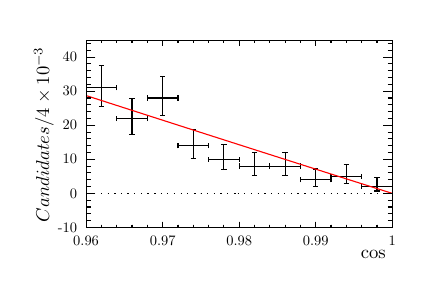
\begin{tikzpicture}
\pgfdeclareplotmark{cross} {
\pgfpathmoveto{\pgfpoint{-0.3\pgfplotmarksize}{\pgfplotmarksize}}
\pgfpathlineto{\pgfpoint{+0.3\pgfplotmarksize}{\pgfplotmarksize}}
\pgfpathlineto{\pgfpoint{+0.3\pgfplotmarksize}{0.3\pgfplotmarksize}}
\pgfpathlineto{\pgfpoint{+1\pgfplotmarksize}{0.3\pgfplotmarksize}}
\pgfpathlineto{\pgfpoint{+1\pgfplotmarksize}{-0.3\pgfplotmarksize}}
\pgfpathlineto{\pgfpoint{+0.3\pgfplotmarksize}{-0.3\pgfplotmarksize}}
\pgfpathlineto{\pgfpoint{+0.3\pgfplotmarksize}{-1.\pgfplotmarksize}}
\pgfpathlineto{\pgfpoint{-0.3\pgfplotmarksize}{-1.\pgfplotmarksize}}
\pgfpathlineto{\pgfpoint{-0.3\pgfplotmarksize}{-0.3\pgfplotmarksize}}
\pgfpathlineto{\pgfpoint{-1.\pgfplotmarksize}{-0.3\pgfplotmarksize}}
\pgfpathlineto{\pgfpoint{-1.\pgfplotmarksize}{0.3\pgfplotmarksize}}
\pgfpathlineto{\pgfpoint{-0.3\pgfplotmarksize}{0.3\pgfplotmarksize}}
\pgfpathclose
\pgfusepathqstroke
}
\pgfdeclareplotmark{cross*} {
\pgfpathmoveto{\pgfpoint{-0.3\pgfplotmarksize}{\pgfplotmarksize}}
\pgfpathlineto{\pgfpoint{+0.3\pgfplotmarksize}{\pgfplotmarksize}}
\pgfpathlineto{\pgfpoint{+0.3\pgfplotmarksize}{0.3\pgfplotmarksize}}
\pgfpathlineto{\pgfpoint{+1\pgfplotmarksize}{0.3\pgfplotmarksize}}
\pgfpathlineto{\pgfpoint{+1\pgfplotmarksize}{-0.3\pgfplotmarksize}}
\pgfpathlineto{\pgfpoint{+0.3\pgfplotmarksize}{-0.3\pgfplotmarksize}}
\pgfpathlineto{\pgfpoint{+0.3\pgfplotmarksize}{-1.\pgfplotmarksize}}
\pgfpathlineto{\pgfpoint{-0.3\pgfplotmarksize}{-1.\pgfplotmarksize}}
\pgfpathlineto{\pgfpoint{-0.3\pgfplotmarksize}{-0.3\pgfplotmarksize}}
\pgfpathlineto{\pgfpoint{-1.\pgfplotmarksize}{-0.3\pgfplotmarksize}}
\pgfpathlineto{\pgfpoint{-1.\pgfplotmarksize}{0.3\pgfplotmarksize}}
\pgfpathlineto{\pgfpoint{-0.3\pgfplotmarksize}{0.3\pgfplotmarksize}}
\pgfpathclose
\pgfusepathqfillstroke
}
\pgfdeclareplotmark{newstar} {
\pgfpathmoveto{\pgfqpoint{0pt}{\pgfplotmarksize}}
\pgfpathlineto{\pgfqpointpolar{44}{0.5\pgfplotmarksize}}
\pgfpathlineto{\pgfqpointpolar{18}{\pgfplotmarksize}}
\pgfpathlineto{\pgfqpointpolar{-20}{0.5\pgfplotmarksize}}
\pgfpathlineto{\pgfqpointpolar{-54}{\pgfplotmarksize}}
\pgfpathlineto{\pgfqpointpolar{-90}{0.5\pgfplotmarksize}}
\pgfpathlineto{\pgfqpointpolar{234}{\pgfplotmarksize}}
\pgfpathlineto{\pgfqpointpolar{198}{0.5\pgfplotmarksize}}
\pgfpathlineto{\pgfqpointpolar{162}{\pgfplotmarksize}}
\pgfpathlineto{\pgfqpointpolar{134}{0.5\pgfplotmarksize}}
\pgfpathclose
\pgfusepathqstroke
}
\pgfdeclareplotmark{newstar*} {
\pgfpathmoveto{\pgfqpoint{0pt}{\pgfplotmarksize}}
\pgfpathlineto{\pgfqpointpolar{44}{0.5\pgfplotmarksize}}
\pgfpathlineto{\pgfqpointpolar{18}{\pgfplotmarksize}}
\pgfpathlineto{\pgfqpointpolar{-20}{0.5\pgfplotmarksize}}
\pgfpathlineto{\pgfqpointpolar{-54}{\pgfplotmarksize}}
\pgfpathlineto{\pgfqpointpolar{-90}{0.5\pgfplotmarksize}}
\pgfpathlineto{\pgfqpointpolar{234}{\pgfplotmarksize}}
\pgfpathlineto{\pgfqpointpolar{198}{0.5\pgfplotmarksize}}
\pgfpathlineto{\pgfqpointpolar{162}{\pgfplotmarksize}}
\pgfpathlineto{\pgfqpointpolar{134}{0.5\pgfplotmarksize}}
\pgfpathclose
\pgfusepathqfillstroke
}
\definecolor{c}{rgb}{1,1,1};
\draw [color=c, fill=c] (0.1,3.20034) rectangle (4.9,6.21242);
\draw [color=c, fill=c] (0.772,3.68227) rectangle (4.66,6.06181);
\definecolor{c}{rgb}{0,0,0};
\draw [c] (0.772,3.68227) -- (0.772,6.06181) -- (4.66,6.06181) -- (4.66,3.68227) -- (0.772,3.68227);
\draw [c,line width=0.4] (0.772,3.68227) -- (4.66,3.68227);
\draw [anchor= east] (4.66,3.34492) node[scale=0.672711, rotate=0]{$\cos\thetaK$};
\draw [c,line width=0.4] (0.772,3.75546) -- (0.772,3.68227);
\draw [c,line width=0.4] (0.9664,3.71887) -- (0.9664,3.68227);
\draw [c,line width=0.4] (1.1608,3.71887) -- (1.1608,3.68227);
\draw [c,line width=0.4] (1.3552,3.71887) -- (1.3552,3.68227);
\draw [c,line width=0.4] (1.5496,3.71887) -- (1.5496,3.68227);
\draw [c,line width=0.4] (1.744,3.75546) -- (1.744,3.68227);
\draw [c,line width=0.4] (1.9384,3.71887) -- (1.9384,3.68227);
\draw [c,line width=0.4] (2.1328,3.71887) -- (2.1328,3.68227);
\draw [c,line width=0.4] (2.3272,3.71887) -- (2.3272,3.68227);
\draw [c,line width=0.4] (2.5216,3.71887) -- (2.5216,3.68227);
\draw [c,line width=0.4] (2.716,3.75546) -- (2.716,3.68227);
\draw [c,line width=0.4] (2.9104,3.71887) -- (2.9104,3.68227);
\draw [c,line width=0.4] (3.1048,3.71887) -- (3.1048,3.68227);
\draw [c,line width=0.4] (3.2992,3.71887) -- (3.2992,3.68227);
\draw [c,line width=0.4] (3.4936,3.71887) -- (3.4936,3.68227);
\draw [c,line width=0.4] (3.688,3.75546) -- (3.688,3.68227);
\draw [c,line width=0.4] (3.8824,3.71887) -- (3.8824,3.68227);
\draw [c,line width=0.4] (4.0768,3.71887) -- (4.0768,3.68227);
\draw [c,line width=0.4] (4.2712,3.71887) -- (4.2712,3.68227);
\draw [c,line width=0.4] (4.4656,3.71887) -- (4.4656,3.68227);
\draw [c,line width=0.4] (4.66,3.75546) -- (4.66,3.68227);
\draw [anchor=base] (0.772,3.45937) node[scale=0.52322, rotate=0]{0.96};
\draw [anchor=base] (1.744,3.45937) node[scale=0.52322, rotate=0]{0.97};
\draw [anchor=base] (2.716,3.45937) node[scale=0.52322, rotate=0]{0.98};
\draw [anchor=base] (3.688,3.45937) node[scale=0.52322, rotate=0]{0.99};
\draw [anchor=base] (4.66,3.45937) node[scale=0.52322, rotate=0]{1};
\draw [c,line width=0.4] (0.772,6.06181) -- (4.66,6.06181);
\draw [c,line width=0.4] (0.772,5.98862) -- (0.772,6.06181);
\draw [c,line width=0.4] (0.9664,6.02522) -- (0.9664,6.06181);
\draw [c,line width=0.4] (1.1608,6.02522) -- (1.1608,6.06181);
\draw [c,line width=0.4] (1.3552,6.02522) -- (1.3552,6.06181);
\draw [c,line width=0.4] (1.5496,6.02522) -- (1.5496,6.06181);
\draw [c,line width=0.4] (1.744,5.98862) -- (1.744,6.06181);
\draw [c,line width=0.4] (1.9384,6.02522) -- (1.9384,6.06181);
\draw [c,line width=0.4] (2.1328,6.02522) -- (2.1328,6.06181);
\draw [c,line width=0.4] (2.3272,6.02522) -- (2.3272,6.06181);
\draw [c,line width=0.4] (2.5216,6.02522) -- (2.5216,6.06181);
\draw [c,line width=0.4] (2.716,5.98862) -- (2.716,6.06181);
\draw [c,line width=0.4] (2.9104,6.02522) -- (2.9104,6.06181);
\draw [c,line width=0.4] (3.1048,6.02522) -- (3.1048,6.06181);
\draw [c,line width=0.4] (3.2992,6.02522) -- (3.2992,6.06181);
\draw [c,line width=0.4] (3.4936,6.02522) -- (3.4936,6.06181);
\draw [c,line width=0.4] (3.688,5.98862) -- (3.688,6.06181);
\draw [c,line width=0.4] (3.8824,6.02522) -- (3.8824,6.06181);
\draw [c,line width=0.4] (4.0768,6.02522) -- (4.0768,6.06181);
\draw [c,line width=0.4] (4.2712,6.02522) -- (4.2712,6.06181);
\draw [c,line width=0.4] (4.4656,6.02522) -- (4.4656,6.06181);
\draw [c,line width=0.4] (4.66,5.98862) -- (4.66,6.06181);
\draw [c,line width=0.4] (0.772,3.68227) -- (0.772,6.06181);
\draw [anchor= east] (0.2344,6.06181) node[scale=0.672711, rotate=90]{$\text{Candidates} / 4\times10^{-3}$};
\draw [c,line width=0.4] (0.88576,3.68227) -- (0.772,3.68227);
\draw [c,line width=0.4] (0.82888,3.7688) -- (0.772,3.7688);
\draw [c,line width=0.4] (0.82888,3.85533) -- (0.772,3.85533);
\draw [c,line width=0.4] (0.82888,3.94186) -- (0.772,3.94186);
\draw [c,line width=0.4] (0.82888,4.02838) -- (0.772,4.02838);
\draw [c,line width=0.4] (0.88576,4.11491) -- (0.772,4.11491);
\draw [c,line width=0.4] (0.82888,4.20144) -- (0.772,4.20144);
\draw [c,line width=0.4] (0.82888,4.28797) -- (0.772,4.28797);
\draw [c,line width=0.4] (0.82888,4.3745) -- (0.772,4.3745);
\draw [c,line width=0.4] (0.82888,4.46103) -- (0.772,4.46103);
\draw [c,line width=0.4] (0.88576,4.54756) -- (0.772,4.54756);
\draw [c,line width=0.4] (0.82888,4.63409) -- (0.772,4.63409);
\draw [c,line width=0.4] (0.82888,4.72061) -- (0.772,4.72061);
\draw [c,line width=0.4] (0.82888,4.80714) -- (0.772,4.80714);
\draw [c,line width=0.4] (0.82888,4.89367) -- (0.772,4.89367);
\draw [c,line width=0.4] (0.88576,4.9802) -- (0.772,4.9802);
\draw [c,line width=0.4] (0.82888,5.06673) -- (0.772,5.06673);
\draw [c,line width=0.4] (0.82888,5.15326) -- (0.772,5.15326);
\draw [c,line width=0.4] (0.82888,5.23979) -- (0.772,5.23979);
\draw [c,line width=0.4] (0.82888,5.32632) -- (0.772,5.32632);
\draw [c,line width=0.4] (0.88576,5.41285) -- (0.772,5.41285);
\draw [c,line width=0.4] (0.82888,5.49937) -- (0.772,5.49937);
\draw [c,line width=0.4] (0.82888,5.5859) -- (0.772,5.5859);
\draw [c,line width=0.4] (0.82888,5.67243) -- (0.772,5.67243);
\draw [c,line width=0.4] (0.82888,5.75896) -- (0.772,5.75896);
\draw [c,line width=0.4] (0.88576,5.84549) -- (0.772,5.84549);
\draw [c,line width=0.4] (0.88576,5.84549) -- (0.772,5.84549);
\draw [c,line width=0.4] (0.82888,5.93202) -- (0.772,5.93202);
\draw [c,line width=0.4] (0.82888,6.01855) -- (0.772,6.01855);
\draw [anchor= east] (0.724,3.68227) node[scale=0.52322, rotate=0]{-10};
\draw [anchor= east] (0.724,4.11491) node[scale=0.52322, rotate=0]{0};
\draw [anchor= east] (0.724,4.54756) node[scale=0.52322, rotate=0]{10};
\draw [anchor= east] (0.724,4.9802) node[scale=0.52322, rotate=0]{20};
\draw [anchor= east] (0.724,5.41285) node[scale=0.52322, rotate=0]{30};
\draw [anchor= east] (0.724,5.84549) node[scale=0.52322, rotate=0]{40};
\draw [c,line width=0.4] (4.66,3.68227) -- (4.66,6.06181);
\draw [c,line width=0.4] (4.54624,3.68227) -- (4.66,3.68227);
\draw [c,line width=0.4] (4.60312,3.7688) -- (4.66,3.7688);
\draw [c,line width=0.4] (4.60312,3.85533) -- (4.66,3.85533);
\draw [c,line width=0.4] (4.60312,3.94186) -- (4.66,3.94186);
\draw [c,line width=0.4] (4.60312,4.02838) -- (4.66,4.02838);
\draw [c,line width=0.4] (4.54624,4.11491) -- (4.66,4.11491);
\draw [c,line width=0.4] (4.60312,4.20144) -- (4.66,4.20144);
\draw [c,line width=0.4] (4.60312,4.28797) -- (4.66,4.28797);
\draw [c,line width=0.4] (4.60312,4.3745) -- (4.66,4.3745);
\draw [c,line width=0.4] (4.60312,4.46103) -- (4.66,4.46103);
\draw [c,line width=0.4] (4.54624,4.54756) -- (4.66,4.54756);
\draw [c,line width=0.4] (4.60312,4.63409) -- (4.66,4.63409);
\draw [c,line width=0.4] (4.60312,4.72061) -- (4.66,4.72061);
\draw [c,line width=0.4] (4.60312,4.80714) -- (4.66,4.80714);
\draw [c,line width=0.4] (4.60312,4.89367) -- (4.66,4.89367);
\draw [c,line width=0.4] (4.54624,4.9802) -- (4.66,4.9802);
\draw [c,line width=0.4] (4.60312,5.06673) -- (4.66,5.06673);
\draw [c,line width=0.4] (4.60312,5.15326) -- (4.66,5.15326);
\draw [c,line width=0.4] (4.60312,5.23979) -- (4.66,5.23979);
\draw [c,line width=0.4] (4.60312,5.32632) -- (4.66,5.32632);
\draw [c,line width=0.4] (4.54624,5.41285) -- (4.66,5.41285);
\draw [c,line width=0.4] (4.60312,5.49937) -- (4.66,5.49937);
\draw [c,line width=0.4] (4.60312,5.5859) -- (4.66,5.5859);
\draw [c,line width=0.4] (4.60312,5.67243) -- (4.66,5.67243);
\draw [c,line width=0.4] (4.60312,5.75896) -- (4.66,5.75896);
\draw [c,line width=0.4] (4.54624,5.84549) -- (4.66,5.84549);
\draw [c,line width=0.4] (4.54624,5.84549) -- (4.66,5.84549);
\draw [c,line width=0.4] (4.60312,5.93202) -- (4.66,5.93202);
\draw [c,line width=0.4] (4.60312,6.01855) -- (4.66,6.01855);
\draw [c,line width=0.4] (0.9664,5.45611) -- (0.772,5.45611);
\draw [c,line width=0.4] (0.772,5.42255) -- (0.772,5.48967);
\draw [c,line width=0.4] (0.9664,5.45611) -- (1.1608,5.45611);
\draw [c,line width=0.4] (1.1608,5.42255) -- (1.1608,5.48967);
\draw [c,line width=0.4] (0.9664,5.45611) -- (0.9664,5.74285);
\draw [c,line width=0.4] (0.932843,5.74285) -- (0.999957,5.74285);
\draw [c,line width=0.4] (0.9664,5.45611) -- (0.9664,5.21653);
\draw [c,line width=0.4] (0.932843,5.21653) -- (0.999957,5.21653);
\draw [c,line width=0.4] (1.3552,5.06673) -- (1.1608,5.06673);
\draw [c,line width=0.4] (1.1608,5.03317) -- (1.1608,5.10029);
\draw [c,line width=0.4] (1.3552,5.06673) -- (1.5496,5.06673);
\draw [c,line width=0.4] (1.5496,5.03317) -- (1.5496,5.10029);
\draw [c,line width=0.4] (1.3552,5.06673) -- (1.3552,5.31599);
\draw [c,line width=0.4] (1.32164,5.31599) -- (1.38876,5.31599);
\draw [c,line width=0.4] (1.3552,5.06673) -- (1.3552,4.86536);
\draw [c,line width=0.4] (1.32164,4.86536) -- (1.38876,4.86536);
\draw [c,line width=0.4] (1.744,5.32632) -- (1.5496,5.32632);
\draw [c,line width=0.4] (1.5496,5.29276) -- (1.5496,5.35987);
\draw [c,line width=0.4] (1.744,5.32632) -- (1.9384,5.32632);
\draw [c,line width=0.4] (1.9384,5.29276) -- (1.9384,5.35987);
\draw [c,line width=0.4] (1.744,5.32632) -- (1.744,5.60124);
\draw [c,line width=0.4] (1.71044,5.60124) -- (1.77756,5.60124);
\draw [c,line width=0.4] (1.744,5.32632) -- (1.744,5.09876);
\draw [c,line width=0.4] (1.71044,5.09876) -- (1.77756,5.09876);
\draw [c,line width=0.4] (2.1328,4.72061) -- (1.9384,4.72061);
\draw [c,line width=0.4] (1.9384,4.68706) -- (1.9384,4.75417);
\draw [c,line width=0.4] (2.1328,4.72061) -- (2.3272,4.72061);
\draw [c,line width=0.4] (2.3272,4.68706) -- (2.3272,4.75417);
\draw [c,line width=0.4] (2.1328,4.72061) -- (2.1328,4.9296);
\draw [c,line width=0.4] (2.09924,4.9296) -- (2.16636,4.9296);
\draw [c,line width=0.4] (2.1328,4.72061) -- (2.1328,4.56069);
\draw [c,line width=0.4] (2.09924,4.56069) -- (2.16636,4.56069);
\draw [c,line width=0.4] (2.5216,4.54756) -- (2.3272,4.54756);
\draw [c,line width=0.4] (2.3272,4.514) -- (2.3272,4.58111);
\draw [c,line width=0.4] (2.5216,4.54756) -- (2.716,4.54756);
\draw [c,line width=0.4] (2.716,4.514) -- (2.716,4.58111);
\draw [c,line width=0.4] (2.5216,4.54756) -- (2.5216,4.73216);
\draw [c,line width=0.4] (2.48804,4.73216) -- (2.55516,4.73216);
\draw [c,line width=0.4] (2.5216,4.54756) -- (2.5216,4.41306);
\draw [c,line width=0.4] (2.48804,4.41306) -- (2.55516,4.41306);
\draw [c,line width=0.4] (2.9104,4.46103) -- (2.716,4.46103);
\draw [c,line width=0.4] (2.716,4.42747) -- (2.716,4.49459);
\draw [c,line width=0.4] (2.9104,4.46103) -- (3.1048,4.46103);
\draw [c,line width=0.4] (3.1048,4.42747) -- (3.1048,4.49459);
\draw [c,line width=0.4] (2.9104,4.46103) -- (2.9104,4.63171);
\draw [c,line width=0.4] (2.87684,4.63171) -- (2.94396,4.63171);
\draw [c,line width=0.4] (2.9104,4.46103) -- (2.9104,4.34126);
\draw [c,line width=0.4] (2.87684,4.34126) -- (2.94396,4.34126);
\draw [c,line width=0.4] (3.2992,4.46103) -- (3.1048,4.46103);
\draw [c,line width=0.4] (3.1048,4.42747) -- (3.1048,4.49459);
\draw [c,line width=0.4] (3.2992,4.46103) -- (3.4936,4.46103);
\draw [c,line width=0.4] (3.4936,4.42747) -- (3.4936,4.49459);
\draw [c,line width=0.4] (3.2992,4.46103) -- (3.2992,4.63171);
\draw [c,line width=0.4] (3.26564,4.63171) -- (3.33276,4.63171);
\draw [c,line width=0.4] (3.2992,4.46103) -- (3.2992,4.34126);
\draw [c,line width=0.4] (3.26564,4.34126) -- (3.33276,4.34126);
\draw [c,line width=0.4] (3.688,4.28797) -- (3.4936,4.28797);
\draw [c,line width=0.4] (3.4936,4.25441) -- (3.4936,4.32153);
\draw [c,line width=0.4] (3.688,4.28797) -- (3.8824,4.28797);
\draw [c,line width=0.4] (3.8824,4.25441) -- (3.8824,4.32153);
\draw [c,line width=0.4] (3.688,4.28797) -- (3.688,4.42481);
\draw [c,line width=0.4] (3.65444,4.42481) -- (3.72156,4.42481);
\draw [c,line width=0.4] (3.688,4.28797) -- (3.688,4.20515);
\draw [c,line width=0.4] (3.65444,4.20515) -- (3.72156,4.20515);
\draw [c,line width=0.4] (4.0768,4.33123) -- (3.8824,4.33123);
\draw [c,line width=0.4] (3.8824,4.29768) -- (3.8824,4.36479);
\draw [c,line width=0.4] (4.0768,4.33123) -- (4.2712,4.33123);
\draw [c,line width=0.4] (4.2712,4.29768) -- (4.2712,4.36479);
\draw [c,line width=0.4] (4.0768,4.33123) -- (4.0768,4.47758);
\draw [c,line width=0.4] (4.04324,4.47758) -- (4.11036,4.47758);
\draw [c,line width=0.4] (4.0768,4.33123) -- (4.0768,4.2378);
\draw [c,line width=0.4] (4.04324,4.2378) -- (4.11036,4.2378);
\draw [c,line width=0.4] (4.4656,4.20144) -- (4.2712,4.20144);
\draw [c,line width=0.4] (4.2712,4.16788) -- (4.2712,4.235);
\draw [c,line width=0.4] (4.4656,4.20144) -- (4.66,4.20144);
\draw [c,line width=0.4] (4.66,4.16788) -- (4.66,4.235);
\draw [c,line width=0.4] (4.4656,4.20144) -- (4.4656,4.31557);
\draw [c,line width=0.4] (4.43204,4.31557) -- (4.49916,4.31557);
\draw [c,line width=0.4] (4.4656,4.20144) -- (4.4656,4.14555);
\draw [c,line width=0.4] (4.43204,4.14555) -- (4.49916,4.14555);
\foreach \P in {(0.9664,5.45611),(1.3552,5.06673),(1.744,5.32632),(2.1328,4.72061),(2.5216,4.54756),(2.9104,4.46103),(3.2992,4.46103),(3.688,4.28797),(4.0768,4.33123),(4.4656,4.20144)}{\draw[mark options={color=c,fill=c},mark size=0.960961pt,mark=]
 plot coordinates {\P};}
\definecolor{c}{rgb}{1,0,0};
\draw [c,line width=0.4] (0.772,5.35728) -- (0.772,5.35728);
\draw [c,line width=0.4] (0.772,5.35728) -- (1.1608,5.23202) -- (1.5496,5.1069) -- (1.9384,4.98194) -- (2.3272,4.85718) -- (2.716,4.73266) -- (3.1048,4.60841) -- (3.4936,4.48447) -- (3.8824,4.36088) -- (4.2712,4.23768) -- (4.66,4.11491) --
 (4.66,4.11491) -- (4.66,4.11491);
\definecolor{c}{rgb}{0,0,0};
\draw [c,line width=0.4] (0.772,3.68227) -- (4.66,3.68227);
\draw [c,line width=0.4] (0.772,3.75546) -- (0.772,3.68227);
\draw [c,line width=0.4] (0.9664,3.71887) -- (0.9664,3.68227);
\draw [c,line width=0.4] (1.1608,3.71887) -- (1.1608,3.68227);
\draw [c,line width=0.4] (1.3552,3.71887) -- (1.3552,3.68227);
\draw [c,line width=0.4] (1.5496,3.71887) -- (1.5496,3.68227);
\draw [c,line width=0.4] (1.744,3.75546) -- (1.744,3.68227);
\draw [c,line width=0.4] (1.9384,3.71887) -- (1.9384,3.68227);
\draw [c,line width=0.4] (2.1328,3.71887) -- (2.1328,3.68227);
\draw [c,line width=0.4] (2.3272,3.71887) -- (2.3272,3.68227);
\draw [c,line width=0.4] (2.5216,3.71887) -- (2.5216,3.68227);
\draw [c,line width=0.4] (2.716,3.75546) -- (2.716,3.68227);
\draw [c,line width=0.4] (2.9104,3.71887) -- (2.9104,3.68227);
\draw [c,line width=0.4] (3.1048,3.71887) -- (3.1048,3.68227);
\draw [c,line width=0.4] (3.2992,3.71887) -- (3.2992,3.68227);
\draw [c,line width=0.4] (3.4936,3.71887) -- (3.4936,3.68227);
\draw [c,line width=0.4] (3.688,3.75546) -- (3.688,3.68227);
\draw [c,line width=0.4] (3.8824,3.71887) -- (3.8824,3.68227);
\draw [c,line width=0.4] (4.0768,3.71887) -- (4.0768,3.68227);
\draw [c,line width=0.4] (4.2712,3.71887) -- (4.2712,3.68227);
\draw [c,line width=0.4] (4.4656,3.71887) -- (4.4656,3.68227);
\draw [c,line width=0.4] (4.66,3.75546) -- (4.66,3.68227);
\draw [c,line width=0.4] (0.772,6.06181) -- (4.66,6.06181);
\draw [c,line width=0.4] (0.772,5.98862) -- (0.772,6.06181);
\draw [c,line width=0.4] (0.9664,6.02522) -- (0.9664,6.06181);
\draw [c,line width=0.4] (1.1608,6.02522) -- (1.1608,6.06181);
\draw [c,line width=0.4] (1.3552,6.02522) -- (1.3552,6.06181);
\draw [c,line width=0.4] (1.5496,6.02522) -- (1.5496,6.06181);
\draw [c,line width=0.4] (1.744,5.98862) -- (1.744,6.06181);
\draw [c,line width=0.4] (1.9384,6.02522) -- (1.9384,6.06181);
\draw [c,line width=0.4] (2.1328,6.02522) -- (2.1328,6.06181);
\draw [c,line width=0.4] (2.3272,6.02522) -- (2.3272,6.06181);
\draw [c,line width=0.4] (2.5216,6.02522) -- (2.5216,6.06181);
\draw [c,line width=0.4] (2.716,5.98862) -- (2.716,6.06181);
\draw [c,line width=0.4] (2.9104,6.02522) -- (2.9104,6.06181);
\draw [c,line width=0.4] (3.1048,6.02522) -- (3.1048,6.06181);
\draw [c,line width=0.4] (3.2992,6.02522) -- (3.2992,6.06181);
\draw [c,line width=0.4] (3.4936,6.02522) -- (3.4936,6.06181);
\draw [c,line width=0.4] (3.688,5.98862) -- (3.688,6.06181);
\draw [c,line width=0.4] (3.8824,6.02522) -- (3.8824,6.06181);
\draw [c,line width=0.4] (4.0768,6.02522) -- (4.0768,6.06181);
\draw [c,line width=0.4] (4.2712,6.02522) -- (4.2712,6.06181);
\draw [c,line width=0.4] (4.4656,6.02522) -- (4.4656,6.06181);
\draw [c,line width=0.4] (4.66,5.98862) -- (4.66,6.06181);
\draw [c,line width=0.4] (0.772,3.68227) -- (0.772,6.06181);
\draw [c,line width=0.4] (0.88576,3.68227) -- (0.772,3.68227);
\draw [c,line width=0.4] (0.82888,3.7688) -- (0.772,3.7688);
\draw [c,line width=0.4] (0.82888,3.85533) -- (0.772,3.85533);
\draw [c,line width=0.4] (0.82888,3.94186) -- (0.772,3.94186);
\draw [c,line width=0.4] (0.82888,4.02838) -- (0.772,4.02838);
\draw [c,line width=0.4] (0.88576,4.11491) -- (0.772,4.11491);
\draw [c,line width=0.4] (0.82888,4.20144) -- (0.772,4.20144);
\draw [c,line width=0.4] (0.82888,4.28797) -- (0.772,4.28797);
\draw [c,line width=0.4] (0.82888,4.3745) -- (0.772,4.3745);
\draw [c,line width=0.4] (0.82888,4.46103) -- (0.772,4.46103);
\draw [c,line width=0.4] (0.88576,4.54756) -- (0.772,4.54756);
\draw [c,line width=0.4] (0.82888,4.63409) -- (0.772,4.63409);
\draw [c,line width=0.4] (0.82888,4.72061) -- (0.772,4.72061);
\draw [c,line width=0.4] (0.82888,4.80714) -- (0.772,4.80714);
\draw [c,line width=0.4] (0.82888,4.89367) -- (0.772,4.89367);
\draw [c,line width=0.4] (0.88576,4.9802) -- (0.772,4.9802);
\draw [c,line width=0.4] (0.82888,5.06673) -- (0.772,5.06673);
\draw [c,line width=0.4] (0.82888,5.15326) -- (0.772,5.15326);
\draw [c,line width=0.4] (0.82888,5.23979) -- (0.772,5.23979);
\draw [c,line width=0.4] (0.82888,5.32632) -- (0.772,5.32632);
\draw [c,line width=0.4] (0.88576,5.41285) -- (0.772,5.41285);
\draw [c,line width=0.4] (0.82888,5.49937) -- (0.772,5.49937);
\draw [c,line width=0.4] (0.82888,5.5859) -- (0.772,5.5859);
\draw [c,line width=0.4] (0.82888,5.67243) -- (0.772,5.67243);
\draw [c,line width=0.4] (0.82888,5.75896) -- (0.772,5.75896);
\draw [c,line width=0.4] (0.88576,5.84549) -- (0.772,5.84549);
\draw [c,line width=0.4] (0.88576,5.84549) -- (0.772,5.84549);
\draw [c,line width=0.4] (0.82888,5.93202) -- (0.772,5.93202);
\draw [c,line width=0.4] (0.82888,6.01855) -- (0.772,6.01855);
\draw [c,line width=0.4] (4.66,3.68227) -- (4.66,6.06181);
\draw [c,line width=0.4] (4.54624,3.68227) -- (4.66,3.68227);
\draw [c,line width=0.4] (4.60312,3.7688) -- (4.66,3.7688);
\draw [c,line width=0.4] (4.60312,3.85533) -- (4.66,3.85533);
\draw [c,line width=0.4] (4.60312,3.94186) -- (4.66,3.94186);
\draw [c,line width=0.4] (4.60312,4.02838) -- (4.66,4.02838);
\draw [c,line width=0.4] (4.54624,4.11491) -- (4.66,4.11491);
\draw [c,line width=0.4] (4.60312,4.20144) -- (4.66,4.20144);
\draw [c,line width=0.4] (4.60312,4.28797) -- (4.66,4.28797);
\draw [c,line width=0.4] (4.60312,4.3745) -- (4.66,4.3745);
\draw [c,line width=0.4] (4.60312,4.46103) -- (4.66,4.46103);
\draw [c,line width=0.4] (4.54624,4.54756) -- (4.66,4.54756);
\draw [c,line width=0.4] (4.60312,4.63409) -- (4.66,4.63409);
\draw [c,line width=0.4] (4.60312,4.72061) -- (4.66,4.72061);
\draw [c,line width=0.4] (4.60312,4.80714) -- (4.66,4.80714);
\draw [c,line width=0.4] (4.60312,4.89367) -- (4.66,4.89367);
\draw [c,line width=0.4] (4.54624,4.9802) -- (4.66,4.9802);
\draw [c,line width=0.4] (4.60312,5.06673) -- (4.66,5.06673);
\draw [c,line width=0.4] (4.60312,5.15326) -- (4.66,5.15326);
\draw [c,line width=0.4] (4.60312,5.23979) -- (4.66,5.23979);
\draw [c,line width=0.4] (4.60312,5.32632) -- (4.66,5.32632);
\draw [c,line width=0.4] (4.54624,5.41285) -- (4.66,5.41285);
\draw [c,line width=0.4] (4.60312,5.49937) -- (4.66,5.49937);
\draw [c,line width=0.4] (4.60312,5.5859) -- (4.66,5.5859);
\draw [c,line width=0.4] (4.60312,5.67243) -- (4.66,5.67243);
\draw [c,line width=0.4] (4.60312,5.75896) -- (4.66,5.75896);
\draw [c,line width=0.4] (4.54624,5.84549) -- (4.66,5.84549);
\draw [c,line width=0.4] (4.54624,5.84549) -- (4.66,5.84549);
\draw [c,line width=0.4] (4.60312,5.93202) -- (4.66,5.93202);
\draw [c,line width=0.4] (4.60312,6.01855) -- (4.66,6.01855);
\draw [c,dotted,line width=0.4] (0.79144,4.11491) -- (0.83032,4.11491) -- (0.8692,4.11491) -- (0.90808,4.11491) -- (0.94696,4.11491) -- (0.98584,4.11491) -- (1.02472,4.11491) -- (1.0636,4.11491) -- (1.10248,4.11491) -- (1.14136,4.11491) --
 (1.18024,4.11491) -- (1.21912,4.11491) -- (1.258,4.11491) -- (1.29688,4.11491) -- (1.33576,4.11491) -- (1.37464,4.11491) -- (1.41352,4.11491) -- (1.4524,4.11491) -- (1.49128,4.11491) -- (1.53016,4.11491) -- (1.56904,4.11491) -- (1.60792,4.11491) --
 (1.6468,4.11491) -- (1.68568,4.11491) -- (1.72456,4.11491) -- (1.76344,4.11491) -- (1.80232,4.11491) -- (1.8412,4.11491) -- (1.88008,4.11491) -- (1.91896,4.11491) -- (1.95784,4.11491) -- (1.99672,4.11491) -- (2.0356,4.11491) -- (2.07448,4.11491) --
 (2.11336,4.11491) -- (2.15224,4.11491) -- (2.19112,4.11491) -- (2.23,4.11491) -- (2.26888,4.11491) -- (2.30776,4.11491) -- (2.34664,4.11491) -- (2.38552,4.11491) -- (2.4244,4.11491) -- (2.46328,4.11491) -- (2.50216,4.11491) -- (2.54104,4.11491) --
 (2.57992,4.11491) -- (2.6188,4.11491) -- (2.65768,4.11491) -- (2.69656,4.11491);
\draw [c,dotted,line width=0.4] (2.69656,4.11491) -- (2.73544,4.11491) -- (2.77432,4.11491) -- (2.8132,4.11491) -- (2.85208,4.11491) -- (2.89096,4.11491) -- (2.92984,4.11491) -- (2.96872,4.11491) -- (3.0076,4.11491) -- (3.04648,4.11491) --
 (3.08536,4.11491) -- (3.12424,4.11491) -- (3.16312,4.11491) -- (3.202,4.11491) -- (3.24088,4.11491) -- (3.27976,4.11491) -- (3.31864,4.11491) -- (3.35752,4.11491) -- (3.3964,4.11491) -- (3.43528,4.11491) -- (3.47416,4.11491) -- (3.51304,4.11491) --
 (3.55192,4.11491) -- (3.5908,4.11491) -- (3.62968,4.11491) -- (3.66856,4.11491) -- (3.70744,4.11491) -- (3.74632,4.11491) -- (3.7852,4.11491) -- (3.82408,4.11491) -- (3.86296,4.11491) -- (3.90184,4.11491) -- (3.94072,4.11491) -- (3.9796,4.11491) --
 (4.01848,4.11491) -- (4.05736,4.11491) -- (4.09624,4.11491) -- (4.13512,4.11491) -- (4.174,4.11491) -- (4.21288,4.11491) -- (4.25176,4.11491) -- (4.29064,4.11491) -- (4.32952,4.11491) -- (4.3684,4.11491) -- (4.40728,4.11491) -- (4.44616,4.11491) --
 (4.48504,4.11491) -- (4.52392,4.11491) -- (4.5628,4.11491) -- (4.60168,4.11491);
\draw [c,dotted,line width=0.4] (4.60168,4.11491) -- (4.64056,4.11491);
\end{tikzpicture}
}
    \caption{}
    \label{angAcc_constr_fit}
  \end{subfigure}
  %% \begin{subfigure}{0.5\textwidth}
  %%   \tikzsetnextfilename{eff_helcosthetaK_neg_all_constr_zoom}
  %%   \scalebox{1.3}{\input{Figures/Chapter4/eff_helcosthetaK_neg_all_constr_zoom}}
  %%   \caption{}
  %%   \label{angAcc_constr}
  %% \end{subfigure}
  \caption{\pdf projection of $\cos\thetaK$ corrected with the angular efficiency function before (left) and after (right)
           constraining its value at $\cos\thetaK=1$, shown as the red curve. The black points show the $\cos\thetaK$
           distribution in the simulated sample. Zooming close to $\cos\thetaK=1$ clearly shows the problematic region.}
  \label{angAcc_constr}
\end{figure}

It is actually not trivial to find a good choice of efficiency moments. Two things are relevant when trying to describe a
distribution with orthogonal functions like $P$ and $Y$. One is the shape of the orthogonal function itself and two the sign and size of the calculated moment.
For example the efficiency term $\moment{1}{0}{0}P_1Y_{00}$ is necessary to describe the drop of efficiency in $\cos\thetaK$ but the size of $\moment{1}{0}{0}$
is too large making the total efficiency function negative. Thus one could add the term $P_3Y_{00}\moment{3}{0}{0}$ where $\moment{3}{0}{0}$ is positive
(see \tabref{eff_moms_table} ) to counter the large negative value of $\moment{1}{0}{0}$ but unfortunately it is not enough. Things get more complicated
when trying to choose efficiency moments that affect the acceptance shape in all of its three dimensions at the same time.

Having chosen the best possible set of moments the efficiency function has to be constrained such that the condition,

\begin{equation}
  \centering
  \epsilon(\cos\thetaK = 1, \cos\thetamu, \phihel) = 0,
  \label{eff_func_constr}
\end{equation}

\noindent is satisfied. It turns out that this condition can be easily satisfied if the basis that the
efficiency function is decomposed, see \equref{eff_func}, is modified as:

\begin{align}
  \centering
   \effbase \to \parenthesis{\effbase}^\prime = \left[\legendre{i}{0}-P_i^0(1)\right] \spharm{j}{k},
  \label{eff_basis_transform}
  \end{align}

\noindent resulting in the following efficiency function:

\begin{align}
    \centering
  \epsilon(\Omega) = \sum_{ijk} \; \moment{i}{j}{k} \; \left[\legendre{i}{0}-P_i^0(1)\right] \; \spharm{j}{k}.
  \label{eff_func_new}
\end{align}

\noindent Note that the subscript $i$ in $P_i^0(1)$ is irrelevant since $P_i^0(1)=1$ for any value of $i$.
The result of the above constraint is shown in \figref{angAcc_constr_fit}, where it can be seen that
the acceptance projection on $\cos\thetaK=1$ is not negative anymore. In addition it has also been checked
whether the acceptance is negative in 2D and 3D, since it is possible for a 2D projection of the acceptance
to take negative values whilst the 1D projections are positive. Two dimensional projection of the constrained
acceptance can be seen in \figref{eff2D}.

\begin{figure}[t]
  \centering
  \begin{subfigure}{0.5\textwidth}
    \raggedright
    \includegraphics[width=\textwidth]{Figures/Chapter4/canv_cosThK_cosThL_Sim08_3fb_hel_negKaons_all.pdf}
    \caption{}
    \label{eff2D_kl}
  \end{subfigure}%
  \hfill%
  \begin{subfigure}{0.5\textwidth}
    \raggedleft
    \includegraphics[width=\textwidth]{Figures/Chapter4/canv_cosThK_phi_Sim08_3fb_hel_negKaons_all.pdf}
    \caption{}
    \label{eff2D_kp}
  \end{subfigure}
  \begin{subfigure}{0.5\textwidth}
    \raggedright
    \includegraphics[width=\textwidth]{Figures/Chapter4/canv_cosThL_phi_Sim08_3fb_hel_negKaons_all.pdf}
    \caption{}
    \label{eff2D_lp}
  \end{subfigure}
\caption{Two dimensional efficiency projections of the constrained efficiency function.
         The equivalent plots for \BsbarJpsiKst are indistinguishable by eye. The scale of the $y$-axis is arbitrary.}
    \label{eff2D}
\end{figure}

Constraining the acceptance in the manner described above comes with a small penalty: the shape of the 1D acceptance
projections is slightly distorted. In order to reduce this distortion and describe better the acceptance shape an additional step is implemented.
As previously mentioned, the acceptance function of \equref{eff_func_new} is fitted to the simulated data
where the efficiency moments are allowed to vary from their measured values, of \tabref{eff_moms_table}.
This feature is implemented by a multivariate Gaussian constraint where correlations between efficiency moments are taken into account.
The fitting \pdf is shown in \equref{mvm_constr} and it consists of the \pdf with which the simulated
data were generated, multiplied with the efficiency function \eqref{eff_func_new} times the multivariate Gaussian constraint.
The physics parameters used to generate the simulation sample are fixed and only the efficiency moments are allowed to vary.
The multivariate Gaussian function $G(\vec{\bf{c}})$, used to constrain the efficiency moments is shown in \equref{mvm_constr_gauss}.

\begin{equation}
  \centering
  \mathcal{P}= \Pgen \times\epsilon(\Omega;\vec{\bf c})  \times G(\vec{\bf{c}}),
  \label{mvm_constr}
\end{equation}

\noindent with

\begin{equation}
\centering
  G(\vec{\bf{c}}) = \frac{1}{\sqrt{(2\pi)^k}|C|} \; e^{-\frac{1}{2}(  \vec{\bf{c}} - <{\bf{c}}>  )^{\text{T}} C^{-1} (\vec{\bf{c}} - <{\bf{c}}> ) },
\label{mvm_constr_gauss}
\end{equation}

\noindent where $\vec{\bf c}$ represents the estimated efficiency moments and $<\vec{\bf c}>$ are the efficiency moments
of \tabref{eff_moms_table}. $C$ and $|C|$ are the covariance matrix of the efficiency moments and its determinant respectively.
Lastly, $k$ is the number of efficiency moments present in \equref{eff_func_new}.

\subsubsection{Alternative parametrization}
As mentioned before there is at least one more way to parameterize the angular acceptance, namely the \emph{normalization weights}.
The main difference between this approach and the method adopted in this analysis is that essentially the normalization weights use the angular functions
of \tabref{ang_distr} as a basis to project the efficiency of \equref{eff_def}, instead of the orthogonal basis $a_i^{jk}$ of \equref{eff_func}.
Looking at \equref{norm_weights_pdf} it is helpful to realize how the normalization weights, $\xi_a$, are introduced into the fitting \pdf.
One can see that they effectively do not multiply the angular \pdf directly. Instead the normalization weights modify the relative contributions
between the angular functions $h_n$, in the normalization integral of the fitting \pdf. The normalization weights are also calculated following the concept of Monte Carlo integration
similarly to the case of efficiency moments.

\begin{equation}
  \mathcal{P} \propto \frac{\sum_n h_n(\Omega)}{\sum_n \int d\Omega \; \epsilon(\Omega) \; h_n(\Omega)}, \;\;\;\;\text{where} \int d\Omega \; \epsilon(\Omega) \; h_n(\Omega) \equiv \xi_a
  \label{norm_weights_pdf}
\end{equation}

The advantages of this method is that it is by construction immune from any issue with localized negative efficiency values:
the acceptance shape is not parameterized at all. The disadvantage on the other hand is that directly
plotting the fitting \pdf becomes impossible when using normalization weights. This is because the normalization integral
of the fitting \pdf is modified in a non-trivial way and other methods need to be implemented in order to visualize the \pdf.
Lastly the two methods can yield identical values on the
fitted parameters by mapping the normalization weights to efficiency moments. This can be done if one solves the normalization integral,
$\int d\Omega\;\Pgen\times\epsilon(\Omega)$ of the \pdf of \tabref{ang_distr} and the efficiency function in \equref{eff_func},
then the mapping of $\moment{i}{j}{k} \rightarrow \xi_a$ follows naturally by exploiting the orthogonality of $P$ and $Y$.
However, the above-mentioned mapping is not unique and not always invertible. It depends on the choice of the particular
efficiency moments. More details on the normalization weights approach can be found in \cite{jeroenThesis} and \cite{tristanThesis}.

%%%%%%%%%%%%%%%%%%%%%%%%%%%%%%%%%%%%%%%%%%%%%%%%
\subsection{Acceptance Corrections}
\label{Accceptance_Corrections}
%%%%%%%%%%%%%%%%%%%%%%%%%%%%%%%%%%%%%%%%%%%%%%%%
The angular acceptance described in section \secref{Accceptance} is determined with simulated \BsJpsiKst events.
Thus the acceptance determination can be trusted only if the simulation accurately describes the detector as well as the
physical amplitudes of the \BsJpsiKst decay. Specifically real and simulated data differences in the momentum distributions
of the final state particles may reflect a different acceptance in real compared to simulated data.
Such differences are at a few percent level between real and simulated data.
On the other hand, differences between data and simulation could be also attributed to
differences in the underlying physical parameter values generating the simulated data compared to these
present in data. For example, the presence of S-wave in the data (and its absence on simulated data)
can cause a difference in the observed kaon momentum spectrum even though the angular acceptance may be perfectly simulated.
Both of the above-mentioned effects have an impact on the decay angles distribution since the helicity angles are functions
of the momenta of the final state particles.

In order to overcome the problem of simulation imperfections, the simulated sample is weighted using an iterative procedure.
At each step of the weighting procedure the simulated data are corrected for the current best estimate of the physics
parameters and the two dimensional $(p_{\kaon},p_{\pion})$ momentum distribution.
The efficiency moments are re-evaluated using the weighted simulated sample and the fit to the data is repeated.
This changes the best estimate of the parameters of interest. This procedure is repeated until these parameters
converge. The full procedure by steps can be summarized as:

\begin{figure}[!t]
  \centering
  \begin{subfigure}{0.49\textwidth}
    \raggedright
    \tikzsetnextfilename{eff_mc_helcosthetaK_allKaons_binall_rew}
    \scalebox{1.13}{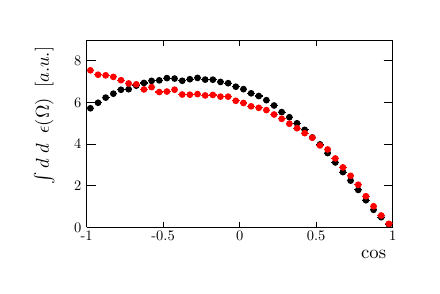
\begin{tikzpicture}
\pgfdeclareplotmark{cross} {
\pgfpathmoveto{\pgfpoint{-0.3\pgfplotmarksize}{\pgfplotmarksize}}
\pgfpathlineto{\pgfpoint{+0.3\pgfplotmarksize}{\pgfplotmarksize}}
\pgfpathlineto{\pgfpoint{+0.3\pgfplotmarksize}{0.3\pgfplotmarksize}}
\pgfpathlineto{\pgfpoint{+1\pgfplotmarksize}{0.3\pgfplotmarksize}}
\pgfpathlineto{\pgfpoint{+1\pgfplotmarksize}{-0.3\pgfplotmarksize}}
\pgfpathlineto{\pgfpoint{+0.3\pgfplotmarksize}{-0.3\pgfplotmarksize}}
\pgfpathlineto{\pgfpoint{+0.3\pgfplotmarksize}{-1.\pgfplotmarksize}}
\pgfpathlineto{\pgfpoint{-0.3\pgfplotmarksize}{-1.\pgfplotmarksize}}
\pgfpathlineto{\pgfpoint{-0.3\pgfplotmarksize}{-0.3\pgfplotmarksize}}
\pgfpathlineto{\pgfpoint{-1.\pgfplotmarksize}{-0.3\pgfplotmarksize}}
\pgfpathlineto{\pgfpoint{-1.\pgfplotmarksize}{0.3\pgfplotmarksize}}
\pgfpathlineto{\pgfpoint{-0.3\pgfplotmarksize}{0.3\pgfplotmarksize}}
\pgfpathclose
\pgfusepathqstroke
}
\pgfdeclareplotmark{cross*} {
\pgfpathmoveto{\pgfpoint{-0.3\pgfplotmarksize}{\pgfplotmarksize}}
\pgfpathlineto{\pgfpoint{+0.3\pgfplotmarksize}{\pgfplotmarksize}}
\pgfpathlineto{\pgfpoint{+0.3\pgfplotmarksize}{0.3\pgfplotmarksize}}
\pgfpathlineto{\pgfpoint{+1\pgfplotmarksize}{0.3\pgfplotmarksize}}
\pgfpathlineto{\pgfpoint{+1\pgfplotmarksize}{-0.3\pgfplotmarksize}}
\pgfpathlineto{\pgfpoint{+0.3\pgfplotmarksize}{-0.3\pgfplotmarksize}}
\pgfpathlineto{\pgfpoint{+0.3\pgfplotmarksize}{-1.\pgfplotmarksize}}
\pgfpathlineto{\pgfpoint{-0.3\pgfplotmarksize}{-1.\pgfplotmarksize}}
\pgfpathlineto{\pgfpoint{-0.3\pgfplotmarksize}{-0.3\pgfplotmarksize}}
\pgfpathlineto{\pgfpoint{-1.\pgfplotmarksize}{-0.3\pgfplotmarksize}}
\pgfpathlineto{\pgfpoint{-1.\pgfplotmarksize}{0.3\pgfplotmarksize}}
\pgfpathlineto{\pgfpoint{-0.3\pgfplotmarksize}{0.3\pgfplotmarksize}}
\pgfpathclose
\pgfusepathqfillstroke
}
\pgfdeclareplotmark{newstar} {
\pgfpathmoveto{\pgfqpoint{0pt}{\pgfplotmarksize}}
\pgfpathlineto{\pgfqpointpolar{44}{0.5\pgfplotmarksize}}
\pgfpathlineto{\pgfqpointpolar{18}{\pgfplotmarksize}}
\pgfpathlineto{\pgfqpointpolar{-20}{0.5\pgfplotmarksize}}
\pgfpathlineto{\pgfqpointpolar{-54}{\pgfplotmarksize}}
\pgfpathlineto{\pgfqpointpolar{-90}{0.5\pgfplotmarksize}}
\pgfpathlineto{\pgfqpointpolar{234}{\pgfplotmarksize}}
\pgfpathlineto{\pgfqpointpolar{198}{0.5\pgfplotmarksize}}
\pgfpathlineto{\pgfqpointpolar{162}{\pgfplotmarksize}}
\pgfpathlineto{\pgfqpointpolar{134}{0.5\pgfplotmarksize}}
\pgfpathclose
\pgfusepathqstroke
}
\pgfdeclareplotmark{newstar*} {
\pgfpathmoveto{\pgfqpoint{0pt}{\pgfplotmarksize}}
\pgfpathlineto{\pgfqpointpolar{44}{0.5\pgfplotmarksize}}
\pgfpathlineto{\pgfqpointpolar{18}{\pgfplotmarksize}}
\pgfpathlineto{\pgfqpointpolar{-20}{0.5\pgfplotmarksize}}
\pgfpathlineto{\pgfqpointpolar{-54}{\pgfplotmarksize}}
\pgfpathlineto{\pgfqpointpolar{-90}{0.5\pgfplotmarksize}}
\pgfpathlineto{\pgfqpointpolar{234}{\pgfplotmarksize}}
\pgfpathlineto{\pgfqpointpolar{198}{0.5\pgfplotmarksize}}
\pgfpathlineto{\pgfqpointpolar{162}{\pgfplotmarksize}}
\pgfpathlineto{\pgfqpointpolar{134}{0.5\pgfplotmarksize}}
\pgfpathclose
\pgfusepathqfillstroke
}
\definecolor{c}{rgb}{1,1,1};
\draw [color=c, fill=c] (0.1,3.20034) rectangle (4.9,6.21242);
\draw [color=c, fill=c] (0.772,3.68227) rectangle (4.66,6.06181);
\definecolor{c}{rgb}{0,0,0};
\draw [c] (0.772,3.68227) -- (0.772,6.06181) -- (4.66,6.06181) -- (4.66,3.68227) -- (0.772,3.68227);
\draw [c,line width=0.4] (0.8206,5.18633) -- (0.8206,5.19592);
\draw [c,line width=0.4] (0.8206,5.19592) -- (0.8206,5.20551);
\draw [c,line width=0.4] (0.772,5.19592) -- (0.8206,5.19592);
\draw [c,line width=0.4] (0.8206,5.19592) -- (0.8692,5.19592);
\foreach \P in {(0.8206,5.19592)}{\draw[mark options={color=c,fill=c},mark size=2.402402pt,mark=*,mark size=1pt] plot coordinates {\P};}
\draw [c,line width=0.4] (0.9178,5.25594) -- (0.9178,5.26575);
\draw [c,line width=0.4] (0.9178,5.26575) -- (0.9178,5.27556);
\draw [c,line width=0.4] (0.8692,5.26575) -- (0.9178,5.26575);
\draw [c,line width=0.4] (0.9178,5.26575) -- (0.9664,5.26575);
\foreach \P in {(0.9178,5.26575)}{\draw[mark options={color=c,fill=c},mark size=2.402402pt,mark=*,mark size=1pt] plot coordinates {\P};}
\draw [c,line width=0.4] (1.015,5.32101) -- (1.015,5.33102);
\draw [c,line width=0.4] (1.015,5.33102) -- (1.015,5.34103);
\draw [c,line width=0.4] (0.9664,5.33102) -- (1.015,5.33102);
\draw [c,line width=0.4] (1.015,5.33102) -- (1.0636,5.33102);
\foreach \P in {(1.015,5.33102)}{\draw[mark options={color=c,fill=c},mark size=2.402402pt,mark=*,mark size=1pt] plot coordinates {\P};}
\draw [c,line width=0.4] (1.1122,5.3709) -- (1.1122,5.38106);
\draw [c,line width=0.4] (1.1122,5.38106) -- (1.1122,5.39123);
\draw [c,line width=0.4] (1.0636,5.38106) -- (1.1122,5.38106);
\draw [c,line width=0.4] (1.1122,5.38106) -- (1.1608,5.38106);
\foreach \P in {(1.1122,5.38106)}{\draw[mark options={color=c,fill=c},mark size=2.402402pt,mark=*,mark size=1pt] plot coordinates {\P};}
\draw [c,line width=0.4] (1.2094,5.42057) -- (1.2094,5.43088);
\draw [c,line width=0.4] (1.2094,5.43088) -- (1.2094,5.44119);
\draw [c,line width=0.4] (1.1608,5.43088) -- (1.2094,5.43088);
\draw [c,line width=0.4] (1.2094,5.43088) -- (1.258,5.43088);
\foreach \P in {(1.2094,5.43088)}{\draw[mark options={color=c,fill=c},mark size=2.402402pt,mark=*,mark size=1pt] plot coordinates {\P};}
\draw [c,line width=0.4] (1.3066,5.42732) -- (1.3066,5.43765);
\draw [c,line width=0.4] (1.3066,5.43765) -- (1.3066,5.44798);
\draw [c,line width=0.4] (1.258,5.43765) -- (1.3066,5.43765);
\draw [c,line width=0.4] (1.3066,5.43765) -- (1.3552,5.43765);
\foreach \P in {(1.3066,5.43765)}{\draw[mark options={color=c,fill=c},mark size=2.402402pt,mark=*,mark size=1pt] plot coordinates {\P};}
\draw [c,line width=0.4] (1.4038,5.47251) -- (1.4038,5.48298);
\draw [c,line width=0.4] (1.4038,5.48298) -- (1.4038,5.49344);
\draw [c,line width=0.4] (1.3552,5.48298) -- (1.4038,5.48298);
\draw [c,line width=0.4] (1.4038,5.48298) -- (1.4524,5.48298);
\foreach \P in {(1.4038,5.48298)}{\draw[mark options={color=c,fill=c},mark size=2.402402pt,mark=*,mark size=1pt] plot coordinates {\P};}
\draw [c,line width=0.4] (1.501,5.50679) -- (1.501,5.51735);
\draw [c,line width=0.4] (1.501,5.51735) -- (1.501,5.52791);
\draw [c,line width=0.4] (1.4524,5.51735) -- (1.501,5.51735);
\draw [c,line width=0.4] (1.501,5.51735) -- (1.5496,5.51735);
\foreach \P in {(1.501,5.51735)}{\draw[mark options={color=c,fill=c},mark size=2.402402pt,mark=*,mark size=1pt] plot coordinates {\P};}
\draw [c,line width=0.4] (1.5982,5.53334) -- (1.5982,5.54397);
\draw [c,line width=0.4] (1.5982,5.54397) -- (1.5982,5.55461);
\draw [c,line width=0.4] (1.5496,5.54397) -- (1.5982,5.54397);
\draw [c,line width=0.4] (1.5982,5.54397) -- (1.6468,5.54397);
\foreach \P in {(1.5982,5.54397)}{\draw[mark options={color=c,fill=c},mark size=2.402402pt,mark=*,mark size=1pt] plot coordinates {\P};}
\draw [c,line width=0.4] (1.6954,5.53996) -- (1.6954,5.55062);
\draw [c,line width=0.4] (1.6954,5.55062) -- (1.6954,5.56128);
\draw [c,line width=0.4] (1.6468,5.55062) -- (1.6954,5.55062);
\draw [c,line width=0.4] (1.6954,5.55062) -- (1.744,5.55062);
\foreach \P in {(1.6954,5.55062)}{\draw[mark options={color=c,fill=c},mark size=2.402402pt,mark=*,mark size=1pt] plot coordinates {\P};}
\draw [c,line width=0.4] (1.7926,5.56786) -- (1.7926,5.5786);
\draw [c,line width=0.4] (1.7926,5.5786) -- (1.7926,5.58934);
\draw [c,line width=0.4] (1.744,5.5786) -- (1.7926,5.5786);
\draw [c,line width=0.4] (1.7926,5.5786) -- (1.8412,5.5786);
\foreach \P in {(1.7926,5.5786)}{\draw[mark options={color=c,fill=c},mark size=2.402402pt,mark=*,mark size=1pt] plot coordinates {\P};}
\draw [c,line width=0.4] (1.8898,5.56224) -- (1.8898,5.57296);
\draw [c,line width=0.4] (1.8898,5.57296) -- (1.8898,5.58368);
\draw [c,line width=0.4] (1.8412,5.57296) -- (1.8898,5.57296);
\draw [c,line width=0.4] (1.8898,5.57296) -- (1.9384,5.57296);
\foreach \P in {(1.8898,5.57296)}{\draw[mark options={color=c,fill=c},mark size=2.402402pt,mark=*,mark size=1pt] plot coordinates {\P};}
\draw [c,line width=0.4] (1.987,5.53446) -- (1.987,5.5451);
\draw [c,line width=0.4] (1.987,5.5451) -- (1.987,5.55574);
\draw [c,line width=0.4] (1.9384,5.5451) -- (1.987,5.5451);
\draw [c,line width=0.4] (1.987,5.5451) -- (2.0356,5.5451);
\foreach \P in {(1.987,5.5451)}{\draw[mark options={color=c,fill=c},mark size=2.402402pt,mark=*,mark size=1pt] plot coordinates {\P};}
\draw [c,line width=0.4] (2.0842,5.55426) -- (2.0842,5.56495);
\draw [c,line width=0.4] (2.0842,5.56495) -- (2.0842,5.57565);
\draw [c,line width=0.4] (2.0356,5.56495) -- (2.0842,5.56495);
\draw [c,line width=0.4] (2.0842,5.56495) -- (2.1328,5.56495);
\foreach \P in {(2.0842,5.56495)}{\draw[mark options={color=c,fill=c},mark size=2.402402pt,mark=*,mark size=1pt] plot coordinates {\P};}
\draw [c,line width=0.4] (2.1814,5.57061) -- (2.1814,5.58136);
\draw [c,line width=0.4] (2.1814,5.58136) -- (2.1814,5.5921);
\draw [c,line width=0.4] (2.1328,5.58136) -- (2.1814,5.58136);
\draw [c,line width=0.4] (2.1814,5.58136) -- (2.23,5.58136);
\foreach \P in {(2.1814,5.58136)}{\draw[mark options={color=c,fill=c},mark size=2.402402pt,mark=*,mark size=1pt] plot coordinates {\P};}
\draw [c,line width=0.4] (2.2786,5.54922) -- (2.2786,5.5599);
\draw [c,line width=0.4] (2.2786,5.5599) -- (2.2786,5.57059);
\draw [c,line width=0.4] (2.23,5.5599) -- (2.2786,5.5599);
\draw [c,line width=0.4] (2.2786,5.5599) -- (2.3272,5.5599);
\foreach \P in {(2.2786,5.5599)}{\draw[mark options={color=c,fill=c},mark size=2.402402pt,mark=*,mark size=1pt] plot coordinates {\P};}
\draw [c,line width=0.4] (2.3758,5.54811) -- (2.3758,5.55879);
\draw [c,line width=0.4] (2.3758,5.55879) -- (2.3758,5.56947);
\draw [c,line width=0.4] (2.3272,5.55879) -- (2.3758,5.55879);
\draw [c,line width=0.4] (2.3758,5.55879) -- (2.4244,5.55879);
\foreach \P in {(2.3758,5.55879)}{\draw[mark options={color=c,fill=c},mark size=2.402402pt,mark=*,mark size=1pt] plot coordinates {\P};}
\draw [c,line width=0.4] (2.473,5.51955) -- (2.473,5.53015);
\draw [c,line width=0.4] (2.473,5.53015) -- (2.473,5.54075);
\draw [c,line width=0.4] (2.4244,5.53015) -- (2.473,5.53015);
\draw [c,line width=0.4] (2.473,5.53015) -- (2.5216,5.53015);
\foreach \P in {(2.473,5.53015)}{\draw[mark options={color=c,fill=c},mark size=2.402402pt,mark=*,mark size=1pt] plot coordinates {\P};}
\draw [c,line width=0.4] (2.5702,5.50366) -- (2.5702,5.51421);
\draw [c,line width=0.4] (2.5702,5.51421) -- (2.5702,5.52476);
\draw [c,line width=0.4] (2.5216,5.51421) -- (2.5702,5.51421);
\draw [c,line width=0.4] (2.5702,5.51421) -- (2.6188,5.51421);
\foreach \P in {(2.5702,5.51421)}{\draw[mark options={color=c,fill=c},mark size=2.402402pt,mark=*,mark size=1pt] plot coordinates {\P};}
\draw [c,line width=0.4] (2.6674,5.4593) -- (2.6674,5.46972);
\draw [c,line width=0.4] (2.6674,5.46972) -- (2.6674,5.48015);
\draw [c,line width=0.4] (2.6188,5.46972) -- (2.6674,5.46972);
\draw [c,line width=0.4] (2.6674,5.46972) -- (2.716,5.46972);
\foreach \P in {(2.6674,5.46972)}{\draw[mark options={color=c,fill=c},mark size=2.402402pt,mark=*,mark size=1pt] plot coordinates {\P};}
\draw [c,line width=0.4] (2.7646,5.42815) -- (2.7646,5.43848);
\draw [c,line width=0.4] (2.7646,5.43848) -- (2.7646,5.44882);
\draw [c,line width=0.4] (2.716,5.43848) -- (2.7646,5.43848);
\draw [c,line width=0.4] (2.7646,5.43848) -- (2.8132,5.43848);
\foreach \P in {(2.7646,5.43848)}{\draw[mark options={color=c,fill=c},mark size=2.402402pt,mark=*,mark size=1pt] plot coordinates {\P};}
\draw [c,line width=0.4] (2.8618,5.37567) -- (2.8618,5.38585);
\draw [c,line width=0.4] (2.8618,5.38585) -- (2.8618,5.39602);
\draw [c,line width=0.4] (2.8132,5.38585) -- (2.8618,5.38585);
\draw [c,line width=0.4] (2.8618,5.38585) -- (2.9104,5.38585);
\foreach \P in {(2.8618,5.38585)}{\draw[mark options={color=c,fill=c},mark size=2.402402pt,mark=*,mark size=1pt] plot coordinates {\P};}
\draw [c,line width=0.4] (2.959,5.34147) -- (2.959,5.35155);
\draw [c,line width=0.4] (2.959,5.35155) -- (2.959,5.36162);
\draw [c,line width=0.4] (2.9104,5.35155) -- (2.959,5.35155);
\draw [c,line width=0.4] (2.959,5.35155) -- (3.0076,5.35155);
\foreach \P in {(2.959,5.35155)}{\draw[mark options={color=c,fill=c},mark size=2.402402pt,mark=*,mark size=1pt] plot coordinates {\P};}
\draw [c,line width=0.4] (3.0562,5.28862) -- (3.0562,5.29854);
\draw [c,line width=0.4] (3.0562,5.29854) -- (3.0562,5.30845);
\draw [c,line width=0.4] (3.0076,5.29854) -- (3.0562,5.29854);
\draw [c,line width=0.4] (3.0562,5.29854) -- (3.1048,5.29854);
\foreach \P in {(3.0562,5.29854)}{\draw[mark options={color=c,fill=c},mark size=2.402402pt,mark=*,mark size=1pt] plot coordinates {\P};}
\draw [c,line width=0.4] (3.1534,5.22121) -- (3.1534,5.23091);
\draw [c,line width=0.4] (3.1534,5.23091) -- (3.1534,5.24061);
\draw [c,line width=0.4] (3.1048,5.23091) -- (3.1534,5.23091);
\draw [c,line width=0.4] (3.1534,5.23091) -- (3.202,5.23091);
\foreach \P in {(3.1534,5.23091)}{\draw[mark options={color=c,fill=c},mark size=2.402402pt,mark=*,mark size=1pt] plot coordinates {\P};}
\draw [c,line width=0.4] (3.2506,5.13778) -- (3.2506,5.14721);
\draw [c,line width=0.4] (3.2506,5.14721) -- (3.2506,5.15665);
\draw [c,line width=0.4] (3.202,5.14721) -- (3.2506,5.14721);
\draw [c,line width=0.4] (3.2506,5.14721) -- (3.2992,5.14721);
\foreach \P in {(3.2506,5.14721)}{\draw[mark options={color=c,fill=c},mark size=2.402402pt,mark=*,mark size=1pt] plot coordinates {\P};}
\draw [c,line width=0.4] (3.3478,5.0726) -- (3.3478,5.08182);
\draw [c,line width=0.4] (3.3478,5.08182) -- (3.3478,5.09105);
\draw [c,line width=0.4] (3.2992,5.08182) -- (3.3478,5.08182);
\draw [c,line width=0.4] (3.3478,5.08182) -- (3.3964,5.08182);
\foreach \P in {(3.3478,5.08182)}{\draw[mark options={color=c,fill=c},mark size=2.402402pt,mark=*,mark size=1pt] plot coordinates {\P};}
\draw [c,line width=0.4] (3.445,4.99639) -- (3.445,5.00536);
\draw [c,line width=0.4] (3.445,5.00536) -- (3.445,5.01433);
\draw [c,line width=0.4] (3.3964,5.00536) -- (3.445,5.00536);
\draw [c,line width=0.4] (3.445,5.00536) -- (3.4936,5.00536);
\foreach \P in {(3.445,5.00536)}{\draw[mark options={color=c,fill=c},mark size=2.402402pt,mark=*,mark size=1pt] plot coordinates {\P};}
\draw [c,line width=0.4] (3.5422,4.9135) -- (3.5422,4.92218);
\draw [c,line width=0.4] (3.5422,4.92218) -- (3.5422,4.93087);
\draw [c,line width=0.4] (3.4936,4.92218) -- (3.5422,4.92218);
\draw [c,line width=0.4] (3.5422,4.92218) -- (3.5908,4.92218);
\foreach \P in {(3.5422,4.92218)}{\draw[mark options={color=c,fill=c},mark size=2.402402pt,mark=*,mark size=1pt] plot coordinates {\P};}
\draw [c,line width=0.4] (3.6394,4.817) -- (3.6394,4.82533);
\draw [c,line width=0.4] (3.6394,4.82533) -- (3.6394,4.83367);
\draw [c,line width=0.4] (3.5908,4.82533) -- (3.6394,4.82533);
\draw [c,line width=0.4] (3.6394,4.82533) -- (3.688,4.82533);
\foreach \P in {(3.6394,4.82533)}{\draw[mark options={color=c,fill=c},mark size=2.402402pt,mark=*,mark size=1pt] plot coordinates {\P};}
\draw [c,line width=0.4] (3.7366,4.72895) -- (3.7366,4.73696);
\draw [c,line width=0.4] (3.7366,4.73696) -- (3.7366,4.74497);
\draw [c,line width=0.4] (3.688,4.73696) -- (3.7366,4.73696);
\draw [c,line width=0.4] (3.7366,4.73696) -- (3.7852,4.73696);
\foreach \P in {(3.7366,4.73696)}{\draw[mark options={color=c,fill=c},mark size=2.402402pt,mark=*,mark size=1pt] plot coordinates {\P};}
\draw [c,line width=0.4] (3.8338,4.61923) -- (3.8338,4.62681);
\draw [c,line width=0.4] (3.8338,4.62681) -- (3.8338,4.63438);
\draw [c,line width=0.4] (3.7852,4.62681) -- (3.8338,4.62681);
\draw [c,line width=0.4] (3.8338,4.62681) -- (3.8824,4.62681);
\foreach \P in {(3.8338,4.62681)}{\draw[mark options={color=c,fill=c},mark size=2.402402pt,mark=*,mark size=1pt] plot coordinates {\P};}
\draw [c,line width=0.4] (3.931,4.50087) -- (3.931,4.50796);
\draw [c,line width=0.4] (3.931,4.50796) -- (3.931,4.51504);
\draw [c,line width=0.4] (3.8824,4.50796) -- (3.931,4.50796);
\draw [c,line width=0.4] (3.931,4.50796) -- (3.9796,4.50796);
\foreach \P in {(3.931,4.50796)}{\draw[mark options={color=c,fill=c},mark size=2.402402pt,mark=*,mark size=1pt] plot coordinates {\P};}
\draw [c,line width=0.4] (4.0282,4.3789) -- (4.0282,4.38544);
\draw [c,line width=0.4] (4.0282,4.38544) -- (4.0282,4.39198);
\draw [c,line width=0.4] (3.9796,4.38544) -- (4.0282,4.38544);
\draw [c,line width=0.4] (4.0282,4.38544) -- (4.0768,4.38544);
\foreach \P in {(4.0282,4.38544)}{\draw[mark options={color=c,fill=c},mark size=2.402402pt,mark=*,mark size=1pt] plot coordinates {\P};}
\draw [c,line width=0.4] (4.1254,4.27109) -- (4.1254,4.2771);
\draw [c,line width=0.4] (4.1254,4.2771) -- (4.1254,4.28311);
\draw [c,line width=0.4] (4.0768,4.2771) -- (4.1254,4.2771);
\draw [c,line width=0.4] (4.1254,4.2771) -- (4.174,4.2771);
\foreach \P in {(4.1254,4.2771)}{\draw[mark options={color=c,fill=c},mark size=2.402402pt,mark=*,mark size=1pt] plot coordinates {\P};}
\draw [c,line width=0.4] (4.2226,4.15326) -- (4.2226,4.15864);
\draw [c,line width=0.4] (4.2226,4.15864) -- (4.2226,4.16402);
\draw [c,line width=0.4] (4.174,4.15864) -- (4.2226,4.15864);
\draw [c,line width=0.4] (4.2226,4.15864) -- (4.2712,4.15864);
\foreach \P in {(4.2226,4.15864)}{\draw[mark options={color=c,fill=c},mark size=2.402402pt,mark=*,mark size=1pt] plot coordinates {\P};}
\draw [c,line width=0.4] (4.3198,4.0232) -- (4.3198,4.02778);
\draw [c,line width=0.4] (4.3198,4.02778) -- (4.3198,4.03237);
\draw [c,line width=0.4] (4.2712,4.02778) -- (4.3198,4.02778);
\draw [c,line width=0.4] (4.3198,4.02778) -- (4.3684,4.02778);
\foreach \P in {(4.3198,4.02778)}{\draw[mark options={color=c,fill=c},mark size=2.402402pt,mark=*,mark size=1pt] plot coordinates {\P};}
\draw [c,line width=0.4] (4.417,3.9027) -- (4.417,3.90639);
\draw [c,line width=0.4] (4.417,3.90639) -- (4.417,3.91008);
\draw [c,line width=0.4] (4.3684,3.90639) -- (4.417,3.90639);
\draw [c,line width=0.4] (4.417,3.90639) -- (4.4656,3.90639);
\foreach \P in {(4.417,3.90639)}{\draw[mark options={color=c,fill=c},mark size=2.402402pt,mark=*,mark size=1pt] plot coordinates {\P};}
\draw [c,line width=0.4] (4.5142,3.80935) -- (4.5142,3.81216);
\draw [c,line width=0.4] (4.5142,3.81216) -- (4.5142,3.81497);
\draw [c,line width=0.4] (4.4656,3.81216) -- (4.5142,3.81216);
\draw [c,line width=0.4] (4.5142,3.81216) -- (4.5628,3.81216);
\foreach \P in {(4.5142,3.81216)}{\draw[mark options={color=c,fill=c},mark size=2.402402pt,mark=*,mark size=1pt] plot coordinates {\P};}
\draw [c,line width=0.4] (4.6114,3.72103) -- (4.6114,3.7226);
\draw [c,line width=0.4] (4.6114,3.7226) -- (4.6114,3.72417);
\draw [c,line width=0.4] (4.5628,3.7226) -- (4.6114,3.7226);
\draw [c,line width=0.4] (4.6114,3.7226) -- (4.66,3.7226);
\foreach \P in {(4.6114,3.7226)}{\draw[mark options={color=c,fill=c},mark size=2.402402pt,mark=*,mark size=1pt] plot coordinates {\P};}
\draw [c,line width=0.4] (0.772,3.68227) -- (4.66,3.68227);
\draw [anchor= east] (4.66,3.34492) node[scale=0.672711, rotate=0]{$\cos\thetaK$};
\draw [c,line width=0.4] (0.772,3.75546) -- (0.772,3.68227);
\draw [c,line width=0.4] (1.744,3.75546) -- (1.744,3.68227);
\draw [c,line width=0.4] (2.716,3.75546) -- (2.716,3.68227);
\draw [c,line width=0.4] (3.688,3.75546) -- (3.688,3.68227);
\draw [c,line width=0.4] (4.66,3.75546) -- (4.66,3.68227);
\draw [anchor=base] (0.772,3.51962) node[scale=0.52322, rotate=0]{-1};
\draw [anchor=base] (1.744,3.51962) node[scale=0.52322, rotate=0]{-0.5};
\draw [anchor=base] (2.716,3.51962) node[scale=0.52322, rotate=0]{0};
\draw [anchor=base] (3.688,3.51962) node[scale=0.52322, rotate=0]{0.5};
\draw [anchor=base] (4.66,3.51962) node[scale=0.52322, rotate=0]{1};
\draw [c,line width=0.4] (0.772,6.06181) -- (4.66,6.06181);
\draw [c,line width=0.4] (0.772,5.98862) -- (0.772,6.06181);
\draw [c,line width=0.4] (1.744,5.98862) -- (1.744,6.06181);
\draw [c,line width=0.4] (2.716,5.98862) -- (2.716,6.06181);
\draw [c,line width=0.4] (3.688,5.98862) -- (3.688,6.06181);
\draw [c,line width=0.4] (4.66,5.98862) -- (4.66,6.06181);
\draw [c,line width=0.4] (0.772,3.68227) -- (0.772,6.06181);
\draw [anchor= east] (0.2344,6.06181) node[scale=0.672711, rotate=90]{$\int d\thetamu \; d\phihel \;\; \epsilon(\Omega) \;\; [\text{a.u.}]$};
\draw [c,line width=0.4] (0.88576,3.68227) -- (0.772,3.68227);
\draw [c,line width=0.4] (0.88576,4.21106) -- (0.772,4.21106);
\draw [c,line width=0.4] (0.88576,4.73984) -- (0.772,4.73984);
\draw [c,line width=0.4] (0.88576,5.26863) -- (0.772,5.26863);
\draw [c,line width=0.4] (0.88576,5.79742) -- (0.772,5.79742);
\draw [c,line width=0.4] (0.88576,5.79742) -- (0.772,5.79742);
\draw [anchor= east] (0.772,3.68227) node[scale=0.52322, rotate=0]{0};
\draw [anchor= east] (0.772,4.21106) node[scale=0.52322, rotate=0]{2};
\draw [anchor= east] (0.772,4.73984) node[scale=0.52322, rotate=0]{4};
\draw [anchor= east] (0.772,5.26863) node[scale=0.52322, rotate=0]{6};
\draw [anchor= east] (0.772,5.79742) node[scale=0.52322, rotate=0]{8};
\draw [c,line width=0.4] (4.66,3.68227) -- (4.66,6.06181);
\draw [c,line width=0.4] (4.54624,3.68227) -- (4.66,3.68227);
\draw [c,line width=0.4] (4.54624,4.21106) -- (4.66,4.21106);
\draw [c,line width=0.4] (4.54624,4.73984) -- (4.66,4.73984);
\draw [c,line width=0.4] (4.54624,5.26863) -- (4.66,5.26863);
\draw [c,line width=0.4] (4.54624,5.79742) -- (4.66,5.79742);
\draw [c,line width=0.4] (4.54624,5.79742) -- (4.66,5.79742);
\definecolor{c}{rgb}{1,0,0};
\draw [c,line width=0.4] (0.8206,5.66676) -- (0.8206,5.67765);
\draw [c,line width=0.4] (0.8206,5.67765) -- (0.8206,5.68855);
\draw [c,line width=0.4] (0.772,5.67765) -- (0.8206,5.67765);
\draw [c,line width=0.4] (0.8206,5.67765) -- (0.8692,5.67765);
\foreach \P in {(0.8206,5.67765)}{\draw[mark options={color=c,fill=c},mark size=2.402402pt,mark=*,mark size=1pt] plot coordinates {\P};}
\draw [c,line width=0.4] (0.9178,5.61113) -- (0.9178,5.62187);
\draw [c,line width=0.4] (0.9178,5.62187) -- (0.9178,5.63261);
\draw [c,line width=0.4] (0.8692,5.62187) -- (0.9178,5.62187);
\draw [c,line width=0.4] (0.9178,5.62187) -- (0.9664,5.62187);
\foreach \P in {(0.9178,5.62187)}{\draw[mark options={color=c,fill=c},mark size=2.402402pt,mark=*,mark size=1pt] plot coordinates {\P};}
\draw [c,line width=0.4] (1.015,5.60355) -- (1.015,5.61427);
\draw [c,line width=0.4] (1.015,5.61427) -- (1.015,5.62499);
\draw [c,line width=0.4] (0.9664,5.61427) -- (1.015,5.61427);
\draw [c,line width=0.4] (1.015,5.61427) -- (1.0636,5.61427);
\foreach \P in {(1.015,5.61427)}{\draw[mark options={color=c,fill=c},mark size=2.402402pt,mark=*,mark size=1pt] plot coordinates {\P};}
\draw [c,line width=0.4] (1.1122,5.5837) -- (1.1122,5.59437);
\draw [c,line width=0.4] (1.1122,5.59437) -- (1.1122,5.60503);
\draw [c,line width=0.4] (1.0636,5.59437) -- (1.1122,5.59437);
\draw [c,line width=0.4] (1.1122,5.59437) -- (1.1608,5.59437);
\foreach \P in {(1.1122,5.59437)}{\draw[mark options={color=c,fill=c},mark size=2.402402pt,mark=*,mark size=1pt] plot coordinates {\P};}
\draw [c,line width=0.4] (1.2094,5.54191) -- (1.2094,5.55245);
\draw [c,line width=0.4] (1.2094,5.55245) -- (1.2094,5.563);
\draw [c,line width=0.4] (1.1608,5.55245) -- (1.2094,5.55245);
\draw [c,line width=0.4] (1.2094,5.55245) -- (1.258,5.55245);
\foreach \P in {(1.2094,5.55245)}{\draw[mark options={color=c,fill=c},mark size=2.402402pt,mark=*,mark size=1pt] plot coordinates {\P};}
\draw [c,line width=0.4] (1.3066,5.50091) -- (1.3066,5.51134);
\draw [c,line width=0.4] (1.3066,5.51134) -- (1.3066,5.52177);
\draw [c,line width=0.4] (1.258,5.51134) -- (1.3066,5.51134);
\draw [c,line width=0.4] (1.3066,5.51134) -- (1.3552,5.51134);
\foreach \P in {(1.3066,5.51134)}{\draw[mark options={color=c,fill=c},mark size=2.402402pt,mark=*,mark size=1pt] plot coordinates {\P};}
\draw [c,line width=0.4] (1.4038,5.48961) -- (1.4038,5.50001);
\draw [c,line width=0.4] (1.4038,5.50001) -- (1.4038,5.51041);
\draw [c,line width=0.4] (1.3552,5.50001) -- (1.4038,5.50001);
\draw [c,line width=0.4] (1.4038,5.50001) -- (1.4524,5.50001);
\foreach \P in {(1.4038,5.50001)}{\draw[mark options={color=c,fill=c},mark size=2.402402pt,mark=*,mark size=1pt] plot coordinates {\P};}
\draw [c,line width=0.4] (1.501,5.42448) -- (1.501,5.43469);
\draw [c,line width=0.4] (1.501,5.43469) -- (1.501,5.4449);
\draw [c,line width=0.4] (1.4524,5.43469) -- (1.501,5.43469);
\draw [c,line width=0.4] (1.501,5.43469) -- (1.5496,5.43469);
\foreach \P in {(1.501,5.43469)}{\draw[mark options={color=c,fill=c},mark size=2.402402pt,mark=*,mark size=1pt] plot coordinates {\P};}
\draw [c,line width=0.4] (1.5982,5.45404) -- (1.5982,5.46433);
\draw [c,line width=0.4] (1.5982,5.46433) -- (1.5982,5.47463);
\draw [c,line width=0.4] (1.5496,5.46433) -- (1.5982,5.46433);
\draw [c,line width=0.4] (1.5982,5.46433) -- (1.6468,5.46433);
\foreach \P in {(1.5982,5.46433)}{\draw[mark options={color=c,fill=c},mark size=2.402402pt,mark=*,mark size=1pt] plot coordinates {\P};}
\draw [c,line width=0.4] (1.6954,5.39176) -- (1.6954,5.40187);
\draw [c,line width=0.4] (1.6954,5.40187) -- (1.6954,5.41199);
\draw [c,line width=0.4] (1.6468,5.40187) -- (1.6954,5.40187);
\draw [c,line width=0.4] (1.6954,5.40187) -- (1.744,5.40187);
\foreach \P in {(1.6954,5.40187)}{\draw[mark options={color=c,fill=c},mark size=2.402402pt,mark=*,mark size=1pt] plot coordinates {\P};}
\draw [c,line width=0.4] (1.7926,5.39825) -- (1.7926,5.40838);
\draw [c,line width=0.4] (1.7926,5.40838) -- (1.7926,5.41851);
\draw [c,line width=0.4] (1.744,5.40838) -- (1.7926,5.40838);
\draw [c,line width=0.4] (1.7926,5.40838) -- (1.8412,5.40838);
\foreach \P in {(1.7926,5.40838)}{\draw[mark options={color=c,fill=c},mark size=2.402402pt,mark=*,mark size=1pt] plot coordinates {\P};}
\draw [c,line width=0.4] (1.8898,5.42137) -- (1.8898,5.43157);
\draw [c,line width=0.4] (1.8898,5.43157) -- (1.8898,5.44177);
\draw [c,line width=0.4] (1.8412,5.43157) -- (1.8898,5.43157);
\draw [c,line width=0.4] (1.8898,5.43157) -- (1.9384,5.43157);
\foreach \P in {(1.8898,5.43157)}{\draw[mark options={color=c,fill=c},mark size=2.402402pt,mark=*,mark size=1pt] plot coordinates {\P};}
\draw [c,line width=0.4] (1.987,5.36013) -- (1.987,5.37016);
\draw [c,line width=0.4] (1.987,5.37016) -- (1.987,5.38018);
\draw [c,line width=0.4] (1.9384,5.37016) -- (1.987,5.37016);
\draw [c,line width=0.4] (1.987,5.37016) -- (2.0356,5.37016);
\foreach \P in {(1.987,5.37016)}{\draw[mark options={color=c,fill=c},mark size=2.402402pt,mark=*,mark size=1pt] plot coordinates {\P};}
\draw [c,line width=0.4] (2.0842,5.35816) -- (2.0842,5.36817);
\draw [c,line width=0.4] (2.0842,5.36817) -- (2.0842,5.37819);
\draw [c,line width=0.4] (2.0356,5.36817) -- (2.0842,5.36817);
\draw [c,line width=0.4] (2.0842,5.36817) -- (2.1328,5.36817);
\foreach \P in {(2.0842,5.36817)}{\draw[mark options={color=c,fill=c},mark size=2.402402pt,mark=*,mark size=1pt] plot coordinates {\P};}
\draw [c,line width=0.4] (2.1814,5.36595) -- (2.1814,5.37599);
\draw [c,line width=0.4] (2.1814,5.37599) -- (2.1814,5.38603);
\draw [c,line width=0.4] (2.1328,5.37599) -- (2.1814,5.37599);
\draw [c,line width=0.4] (2.1814,5.37599) -- (2.23,5.37599);
\foreach \P in {(2.1814,5.37599)}{\draw[mark options={color=c,fill=c},mark size=2.402402pt,mark=*,mark size=1pt] plot coordinates {\P};}
\draw [c,line width=0.4] (2.2786,5.34866) -- (2.2786,5.35865);
\draw [c,line width=0.4] (2.2786,5.35865) -- (2.2786,5.36864);
\draw [c,line width=0.4] (2.23,5.35865) -- (2.2786,5.35865);
\draw [c,line width=0.4] (2.2786,5.35865) -- (2.3272,5.35865);
\foreach \P in {(2.2786,5.35865)}{\draw[mark options={color=c,fill=c},mark size=2.402402pt,mark=*,mark size=1pt] plot coordinates {\P};}
\draw [c,line width=0.4] (2.3758,5.35491) -- (2.3758,5.36492);
\draw [c,line width=0.4] (2.3758,5.36492) -- (2.3758,5.37492);
\draw [c,line width=0.4] (2.3272,5.36492) -- (2.3758,5.36492);
\draw [c,line width=0.4] (2.3758,5.36492) -- (2.4244,5.36492);
\foreach \P in {(2.3758,5.36492)}{\draw[mark options={color=c,fill=c},mark size=2.402402pt,mark=*,mark size=1pt] plot coordinates {\P};}
\draw [c,line width=0.4] (2.473,5.33363) -- (2.473,5.34358);
\draw [c,line width=0.4] (2.473,5.34358) -- (2.473,5.35352);
\draw [c,line width=0.4] (2.4244,5.34358) -- (2.473,5.34358);
\draw [c,line width=0.4] (2.473,5.34358) -- (2.5216,5.34358);
\foreach \P in {(2.473,5.34358)}{\draw[mark options={color=c,fill=c},mark size=2.402402pt,mark=*,mark size=1pt] plot coordinates {\P};}
\draw [c,line width=0.4] (2.5702,5.33345) -- (2.5702,5.34339);
\draw [c,line width=0.4] (2.5702,5.34339) -- (2.5702,5.35333);
\draw [c,line width=0.4] (2.5216,5.34339) -- (2.5702,5.34339);
\draw [c,line width=0.4] (2.5702,5.34339) -- (2.6188,5.34339);
\foreach \P in {(2.5702,5.34339)}{\draw[mark options={color=c,fill=c},mark size=2.402402pt,mark=*,mark size=1pt] plot coordinates {\P};}
\draw [c,line width=0.4] (2.6674,5.28107) -- (2.6674,5.29085);
\draw [c,line width=0.4] (2.6674,5.29085) -- (2.6674,5.30063);
\draw [c,line width=0.4] (2.6188,5.29085) -- (2.6674,5.29085);
\draw [c,line width=0.4] (2.6674,5.29085) -- (2.716,5.29085);
\foreach \P in {(2.6674,5.29085)}{\draw[mark options={color=c,fill=c},mark size=2.402402pt,mark=*,mark size=1pt] plot coordinates {\P};}
\draw [c,line width=0.4] (2.7646,5.25318) -- (2.7646,5.26288);
\draw [c,line width=0.4] (2.7646,5.26288) -- (2.7646,5.27258);
\draw [c,line width=0.4] (2.716,5.26288) -- (2.7646,5.26288);
\draw [c,line width=0.4] (2.7646,5.26288) -- (2.8132,5.26288);
\foreach \P in {(2.7646,5.26288)}{\draw[mark options={color=c,fill=c},mark size=2.402402pt,mark=*,mark size=1pt] plot coordinates {\P};}
\draw [c,line width=0.4] (2.8618,5.21069) -- (2.8618,5.22026);
\draw [c,line width=0.4] (2.8618,5.22026) -- (2.8618,5.22982);
\draw [c,line width=0.4] (2.8132,5.22026) -- (2.8618,5.22026);
\draw [c,line width=0.4] (2.8618,5.22026) -- (2.9104,5.22026);
\foreach \P in {(2.8618,5.22026)}{\draw[mark options={color=c,fill=c},mark size=2.402402pt,mark=*,mark size=1pt] plot coordinates {\P};}
\draw [c,line width=0.4] (2.959,5.19168) -- (2.959,5.20119);
\draw [c,line width=0.4] (2.959,5.20119) -- (2.959,5.21069);
\draw [c,line width=0.4] (2.9104,5.20119) -- (2.959,5.20119);
\draw [c,line width=0.4] (2.959,5.20119) -- (3.0076,5.20119);
\foreach \P in {(2.959,5.20119)}{\draw[mark options={color=c,fill=c},mark size=2.402402pt,mark=*,mark size=1pt] plot coordinates {\P};}
\draw [c,line width=0.4] (3.0562,5.16326) -- (3.0562,5.17268);
\draw [c,line width=0.4] (3.0562,5.17268) -- (3.0562,5.18209);
\draw [c,line width=0.4] (3.0076,5.17268) -- (3.0562,5.17268);
\draw [c,line width=0.4] (3.0562,5.17268) -- (3.1048,5.17268);
\foreach \P in {(3.0562,5.17268)}{\draw[mark options={color=c,fill=c},mark size=2.402402pt,mark=*,mark size=1pt] plot coordinates {\P};}
\draw [c,line width=0.4] (3.1534,5.1075) -- (3.1534,5.11674);
\draw [c,line width=0.4] (3.1534,5.11674) -- (3.1534,5.12598);
\draw [c,line width=0.4] (3.1048,5.11674) -- (3.1534,5.11674);
\draw [c,line width=0.4] (3.1534,5.11674) -- (3.202,5.11674);
\foreach \P in {(3.1534,5.11674)}{\draw[mark options={color=c,fill=c},mark size=2.402402pt,mark=*,mark size=1pt] plot coordinates {\P};}
\draw [c,line width=0.4] (3.2506,5.05247) -- (3.2506,5.06153);
\draw [c,line width=0.4] (3.2506,5.06153) -- (3.2506,5.07059);
\draw [c,line width=0.4] (3.202,5.06153) -- (3.2506,5.06153);
\draw [c,line width=0.4] (3.2506,5.06153) -- (3.2992,5.06153);
\foreach \P in {(3.2506,5.06153)}{\draw[mark options={color=c,fill=c},mark size=2.402402pt,mark=*,mark size=1pt] plot coordinates {\P};}
\draw [c,line width=0.4] (3.3478,4.9909) -- (3.3478,4.99976);
\draw [c,line width=0.4] (3.3478,4.99976) -- (3.3478,5.00861);
\draw [c,line width=0.4] (3.2992,4.99976) -- (3.3478,4.99976);
\draw [c,line width=0.4] (3.3478,4.99976) -- (3.3964,4.99976);
\foreach \P in {(3.3478,4.99976)}{\draw[mark options={color=c,fill=c},mark size=2.402402pt,mark=*,mark size=1pt] plot coordinates {\P};}
\draw [c,line width=0.4] (3.445,4.93385) -- (3.445,4.9425);
\draw [c,line width=0.4] (3.445,4.9425) -- (3.445,4.95116);
\draw [c,line width=0.4] (3.3964,4.9425) -- (3.445,4.9425);
\draw [c,line width=0.4] (3.445,4.9425) -- (3.4936,4.9425);
\foreach \P in {(3.445,4.9425)}{\draw[mark options={color=c,fill=c},mark size=2.402402pt,mark=*,mark size=1pt] plot coordinates {\P};}
\draw [c,line width=0.4] (3.5422,4.87145) -- (3.5422,4.87989);
\draw [c,line width=0.4] (3.5422,4.87989) -- (3.5422,4.88833);
\draw [c,line width=0.4] (3.4936,4.87989) -- (3.5422,4.87989);
\draw [c,line width=0.4] (3.5422,4.87989) -- (3.5908,4.87989);
\foreach \P in {(3.5422,4.87989)}{\draw[mark options={color=c,fill=c},mark size=2.402402pt,mark=*,mark size=1pt] plot coordinates {\P};}
\draw [c,line width=0.4] (3.6394,4.81431) -- (3.6394,4.82255);
\draw [c,line width=0.4] (3.6394,4.82255) -- (3.6394,4.83078);
\draw [c,line width=0.4] (3.5908,4.82255) -- (3.6394,4.82255);
\draw [c,line width=0.4] (3.6394,4.82255) -- (3.688,4.82255);
\foreach \P in {(3.6394,4.82255)}{\draw[mark options={color=c,fill=c},mark size=2.402402pt,mark=*,mark size=1pt] plot coordinates {\P};}
\draw [c,line width=0.4] (3.7366,4.71619) -- (3.7366,4.72406);
\draw [c,line width=0.4] (3.7366,4.72406) -- (3.7366,4.73193);
\draw [c,line width=0.4] (3.688,4.72406) -- (3.7366,4.72406);
\draw [c,line width=0.4] (3.7366,4.72406) -- (3.7852,4.72406);
\foreach \P in {(3.7366,4.72406)}{\draw[mark options={color=c,fill=c},mark size=2.402402pt,mark=*,mark size=1pt] plot coordinates {\P};}
\draw [c,line width=0.4] (3.8338,4.66508) -- (3.8338,4.67276);
\draw [c,line width=0.4] (3.8338,4.67276) -- (3.8338,4.68044);
\draw [c,line width=0.4] (3.7852,4.67276) -- (3.8338,4.67276);
\draw [c,line width=0.4] (3.8338,4.67276) -- (3.8824,4.67276);
\foreach \P in {(3.8338,4.67276)}{\draw[mark options={color=c,fill=c},mark size=2.402402pt,mark=*,mark size=1pt] plot coordinates {\P};}
\draw [c,line width=0.4] (3.931,4.5512) -- (3.931,4.55842);
\draw [c,line width=0.4] (3.931,4.55842) -- (3.931,4.56564);
\draw [c,line width=0.4] (3.8824,4.55842) -- (3.931,4.55842);
\draw [c,line width=0.4] (3.931,4.55842) -- (3.9796,4.55842);
\foreach \P in {(3.931,4.55842)}{\draw[mark options={color=c,fill=c},mark size=2.402402pt,mark=*,mark size=1pt] plot coordinates {\P};}
\draw [c,line width=0.4] (4.0282,4.43834) -- (4.0282,4.44508);
\draw [c,line width=0.4] (4.0282,4.44508) -- (4.0282,4.45182);
\draw [c,line width=0.4] (3.9796,4.44508) -- (4.0282,4.44508);
\draw [c,line width=0.4] (4.0282,4.44508) -- (4.0768,4.44508);
\foreach \P in {(4.0282,4.44508)}{\draw[mark options={color=c,fill=c},mark size=2.402402pt,mark=*,mark size=1pt] plot coordinates {\P};}
\draw [c,line width=0.4] (4.1254,4.33181) -- (4.1254,4.33806);
\draw [c,line width=0.4] (4.1254,4.33806) -- (4.1254,4.34431);
\draw [c,line width=0.4] (4.0768,4.33806) -- (4.1254,4.33806);
\draw [c,line width=0.4] (4.1254,4.33806) -- (4.174,4.33806);
\foreach \P in {(4.1254,4.33806)}{\draw[mark options={color=c,fill=c},mark size=2.402402pt,mark=*,mark size=1pt] plot coordinates {\P};}
\draw [c,line width=0.4] (4.2226,4.21942) -- (4.2226,4.2251);
\draw [c,line width=0.4] (4.2226,4.2251) -- (4.2226,4.23078);
\draw [c,line width=0.4] (4.174,4.2251) -- (4.2226,4.2251);
\draw [c,line width=0.4] (4.2226,4.2251) -- (4.2712,4.2251);
\foreach \P in {(4.2226,4.2251)}{\draw[mark options={color=c,fill=c},mark size=2.402402pt,mark=*,mark size=1pt] plot coordinates {\P};}
\draw [c,line width=0.4] (4.3198,4.0743) -- (4.3198,4.07915);
\draw [c,line width=0.4] (4.3198,4.07915) -- (4.3198,4.08401);
\draw [c,line width=0.4] (4.2712,4.07915) -- (4.3198,4.07915);
\draw [c,line width=0.4] (4.3198,4.07915) -- (4.3684,4.07915);
\foreach \P in {(4.3198,4.07915)}{\draw[mark options={color=c,fill=c},mark size=2.402402pt,mark=*,mark size=1pt] plot coordinates {\P};}
\draw [c,line width=0.4] (4.417,3.94714) -- (4.417,3.95114);
\draw [c,line width=0.4] (4.417,3.95114) -- (4.417,3.95514);
\draw [c,line width=0.4] (4.3684,3.95114) -- (4.417,3.95114);
\draw [c,line width=0.4] (4.417,3.95114) -- (4.4656,3.95114);
\foreach \P in {(4.417,3.95114)}{\draw[mark options={color=c,fill=c},mark size=2.402402pt,mark=*,mark size=1pt] plot coordinates {\P};}
\draw [c,line width=0.4] (4.5142,3.83115) -- (4.5142,3.83415);
\draw [c,line width=0.4] (4.5142,3.83415) -- (4.5142,3.83716);
\draw [c,line width=0.4] (4.4656,3.83415) -- (4.5142,3.83415);
\draw [c,line width=0.4] (4.5142,3.83415) -- (4.5628,3.83415);
\foreach \P in {(4.5142,3.83415)}{\draw[mark options={color=c,fill=c},mark size=2.402402pt,mark=*,mark size=1pt] plot coordinates {\P};}
\draw [c,line width=0.4] (4.6114,3.72672) -- (4.6114,3.72838);
\draw [c,line width=0.4] (4.6114,3.72838) -- (4.6114,3.73004);
\draw [c,line width=0.4] (4.5628,3.72838) -- (4.6114,3.72838);
\draw [c,line width=0.4] (4.6114,3.72838) -- (4.66,3.72838);
\foreach \P in {(4.6114,3.72838)}{\draw[mark options={color=c,fill=c},mark size=2.402402pt,mark=*,mark size=1pt] plot coordinates {\P};}
\end{tikzpicture}
}
    \caption{}
    \label{angAccCor_ctk}
  \end{subfigure}%
  \hfill%
  \begin{subfigure}{0.49\textwidth}
    \raggedleft
    \tikzsetnextfilename{eff_mc_helcosthetaL_allKaons_binall_rew}
    \scalebox{1.13}{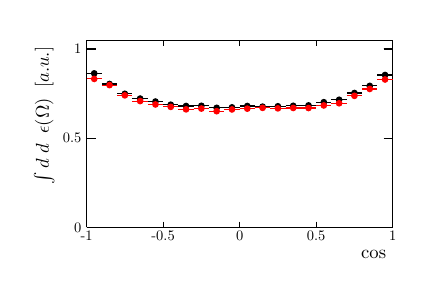
\begin{tikzpicture}
\pgfdeclareplotmark{cross} {
\pgfpathmoveto{\pgfpoint{-0.3\pgfplotmarksize}{\pgfplotmarksize}}
\pgfpathlineto{\pgfpoint{+0.3\pgfplotmarksize}{\pgfplotmarksize}}
\pgfpathlineto{\pgfpoint{+0.3\pgfplotmarksize}{0.3\pgfplotmarksize}}
\pgfpathlineto{\pgfpoint{+1\pgfplotmarksize}{0.3\pgfplotmarksize}}
\pgfpathlineto{\pgfpoint{+1\pgfplotmarksize}{-0.3\pgfplotmarksize}}
\pgfpathlineto{\pgfpoint{+0.3\pgfplotmarksize}{-0.3\pgfplotmarksize}}
\pgfpathlineto{\pgfpoint{+0.3\pgfplotmarksize}{-1.\pgfplotmarksize}}
\pgfpathlineto{\pgfpoint{-0.3\pgfplotmarksize}{-1.\pgfplotmarksize}}
\pgfpathlineto{\pgfpoint{-0.3\pgfplotmarksize}{-0.3\pgfplotmarksize}}
\pgfpathlineto{\pgfpoint{-1.\pgfplotmarksize}{-0.3\pgfplotmarksize}}
\pgfpathlineto{\pgfpoint{-1.\pgfplotmarksize}{0.3\pgfplotmarksize}}
\pgfpathlineto{\pgfpoint{-0.3\pgfplotmarksize}{0.3\pgfplotmarksize}}
\pgfpathclose
\pgfusepathqstroke
}
\pgfdeclareplotmark{cross*} {
\pgfpathmoveto{\pgfpoint{-0.3\pgfplotmarksize}{\pgfplotmarksize}}
\pgfpathlineto{\pgfpoint{+0.3\pgfplotmarksize}{\pgfplotmarksize}}
\pgfpathlineto{\pgfpoint{+0.3\pgfplotmarksize}{0.3\pgfplotmarksize}}
\pgfpathlineto{\pgfpoint{+1\pgfplotmarksize}{0.3\pgfplotmarksize}}
\pgfpathlineto{\pgfpoint{+1\pgfplotmarksize}{-0.3\pgfplotmarksize}}
\pgfpathlineto{\pgfpoint{+0.3\pgfplotmarksize}{-0.3\pgfplotmarksize}}
\pgfpathlineto{\pgfpoint{+0.3\pgfplotmarksize}{-1.\pgfplotmarksize}}
\pgfpathlineto{\pgfpoint{-0.3\pgfplotmarksize}{-1.\pgfplotmarksize}}
\pgfpathlineto{\pgfpoint{-0.3\pgfplotmarksize}{-0.3\pgfplotmarksize}}
\pgfpathlineto{\pgfpoint{-1.\pgfplotmarksize}{-0.3\pgfplotmarksize}}
\pgfpathlineto{\pgfpoint{-1.\pgfplotmarksize}{0.3\pgfplotmarksize}}
\pgfpathlineto{\pgfpoint{-0.3\pgfplotmarksize}{0.3\pgfplotmarksize}}
\pgfpathclose
\pgfusepathqfillstroke
}
\pgfdeclareplotmark{newstar} {
\pgfpathmoveto{\pgfqpoint{0pt}{\pgfplotmarksize}}
\pgfpathlineto{\pgfqpointpolar{44}{0.5\pgfplotmarksize}}
\pgfpathlineto{\pgfqpointpolar{18}{\pgfplotmarksize}}
\pgfpathlineto{\pgfqpointpolar{-20}{0.5\pgfplotmarksize}}
\pgfpathlineto{\pgfqpointpolar{-54}{\pgfplotmarksize}}
\pgfpathlineto{\pgfqpointpolar{-90}{0.5\pgfplotmarksize}}
\pgfpathlineto{\pgfqpointpolar{234}{\pgfplotmarksize}}
\pgfpathlineto{\pgfqpointpolar{198}{0.5\pgfplotmarksize}}
\pgfpathlineto{\pgfqpointpolar{162}{\pgfplotmarksize}}
\pgfpathlineto{\pgfqpointpolar{134}{0.5\pgfplotmarksize}}
\pgfpathclose
\pgfusepathqstroke
}
\pgfdeclareplotmark{newstar*} {
\pgfpathmoveto{\pgfqpoint{0pt}{\pgfplotmarksize}}
\pgfpathlineto{\pgfqpointpolar{44}{0.5\pgfplotmarksize}}
\pgfpathlineto{\pgfqpointpolar{18}{\pgfplotmarksize}}
\pgfpathlineto{\pgfqpointpolar{-20}{0.5\pgfplotmarksize}}
\pgfpathlineto{\pgfqpointpolar{-54}{\pgfplotmarksize}}
\pgfpathlineto{\pgfqpointpolar{-90}{0.5\pgfplotmarksize}}
\pgfpathlineto{\pgfqpointpolar{234}{\pgfplotmarksize}}
\pgfpathlineto{\pgfqpointpolar{198}{0.5\pgfplotmarksize}}
\pgfpathlineto{\pgfqpointpolar{162}{\pgfplotmarksize}}
\pgfpathlineto{\pgfqpointpolar{134}{0.5\pgfplotmarksize}}
\pgfpathclose
\pgfusepathqfillstroke
}
\definecolor{c}{rgb}{1,1,1};
\draw [color=c, fill=c] (5.1,3.20034) rectangle (9.9,6.21242);
\draw [color=c, fill=c] (5.772,3.68227) rectangle (9.66,6.06181);
\definecolor{c}{rgb}{0,0,0};
\draw [c] (5.772,3.68227) -- (5.772,6.06181) -- (9.66,6.06181) -- (9.66,3.68227) -- (5.772,3.68227);
\draw [c,line width=0.4] (5.8692,5.62691) -- (5.8692,5.63874);
\draw [c,line width=0.4] (5.8692,5.63874) -- (5.8692,5.65057);
\draw [c,line width=0.4] (5.772,5.63874) -- (5.8692,5.63874);
\draw [c,line width=0.4] (5.8692,5.63874) -- (5.9664,5.63874);
\foreach \P in {(5.8692,5.63874)}{\draw[mark options={color=c,fill=c},mark size=2.402402pt,mark=*,mark size=1pt] plot coordinates {\P};}
\draw [c,line width=0.4] (6.0636,5.49391) -- (6.0636,5.50447);
\draw [c,line width=0.4] (6.0636,5.50447) -- (6.0636,5.51502);
\draw [c,line width=0.4] (5.9664,5.50447) -- (6.0636,5.50447);
\draw [c,line width=0.4] (6.0636,5.50447) -- (6.1608,5.50447);
\foreach \P in {(6.0636,5.50447)}{\draw[mark options={color=c,fill=c},mark size=2.402402pt,mark=*,mark size=1pt] plot coordinates {\P};}
\draw [c,line width=0.4] (6.258,5.36949) -- (6.258,5.37943);
\draw [c,line width=0.4] (6.258,5.37943) -- (6.258,5.38937);
\draw [c,line width=0.4] (6.1608,5.37943) -- (6.258,5.37943);
\draw [c,line width=0.4] (6.258,5.37943) -- (6.3552,5.37943);
\foreach \P in {(6.258,5.37943)}{\draw[mark options={color=c,fill=c},mark size=2.402402pt,mark=*,mark size=1pt] plot coordinates {\P};}
\draw [c,line width=0.4] (6.4524,5.30891) -- (6.4524,5.31858);
\draw [c,line width=0.4] (6.4524,5.31858) -- (6.4524,5.32825);
\draw [c,line width=0.4] (6.3552,5.31858) -- (6.4524,5.31858);
\draw [c,line width=0.4] (6.4524,5.31858) -- (6.5496,5.31858);
\foreach \P in {(6.4524,5.31858)}{\draw[mark options={color=c,fill=c},mark size=2.402402pt,mark=*,mark size=1pt] plot coordinates {\P};}
\draw [c,line width=0.4] (6.6468,5.27176) -- (6.6468,5.2813);
\draw [c,line width=0.4] (6.6468,5.2813) -- (6.6468,5.29083);
\draw [c,line width=0.4] (6.5496,5.2813) -- (6.6468,5.2813);
\draw [c,line width=0.4] (6.6468,5.2813) -- (6.744,5.2813);
\foreach \P in {(6.6468,5.2813)}{\draw[mark options={color=c,fill=c},mark size=2.402402pt,mark=*,mark size=1pt] plot coordinates {\P};}
\draw [c,line width=0.4] (6.8412,5.23139) -- (6.8412,5.24083);
\draw [c,line width=0.4] (6.8412,5.24083) -- (6.8412,5.25027);
\draw [c,line width=0.4] (6.744,5.24083) -- (6.8412,5.24083);
\draw [c,line width=0.4] (6.8412,5.24083) -- (6.9384,5.24083);
\foreach \P in {(6.8412,5.24083)}{\draw[mark options={color=c,fill=c},mark size=2.402402pt,mark=*,mark size=1pt] plot coordinates {\P};}
\draw [c,line width=0.4] (7.0356,5.21504) -- (7.0356,5.22447);
\draw [c,line width=0.4] (7.0356,5.22447) -- (7.0356,5.2339);
\draw [c,line width=0.4] (6.9384,5.22447) -- (7.0356,5.22447);
\draw [c,line width=0.4] (7.0356,5.22447) -- (7.1328,5.22447);
\foreach \P in {(7.0356,5.22447)}{\draw[mark options={color=c,fill=c},mark size=2.402402pt,mark=*,mark size=1pt] plot coordinates {\P};}
\draw [c,line width=0.4] (7.23,5.21749) -- (7.23,5.22703);
\draw [c,line width=0.4] (7.23,5.22703) -- (7.23,5.23658);
\draw [c,line width=0.4] (7.1328,5.22703) -- (7.23,5.22703);
\draw [c,line width=0.4] (7.23,5.22703) -- (7.3272,5.22703);
\foreach \P in {(7.23,5.22703)}{\draw[mark options={color=c,fill=c},mark size=2.402402pt,mark=*,mark size=1pt] plot coordinates {\P};}
\draw [c,line width=0.4] (7.4244,5.19173) -- (7.4244,5.20122);
\draw [c,line width=0.4] (7.4244,5.20122) -- (7.4244,5.21071);
\draw [c,line width=0.4] (7.3272,5.20122) -- (7.4244,5.20122);
\draw [c,line width=0.4] (7.4244,5.20122) -- (7.5216,5.20122);
\foreach \P in {(7.4244,5.20122)}{\draw[mark options={color=c,fill=c},mark size=2.402402pt,mark=*,mark size=1pt] plot coordinates {\P};}
\draw [c,line width=0.4] (7.6188,5.19782) -- (7.6188,5.20735);
\draw [c,line width=0.4] (7.6188,5.20735) -- (7.6188,5.21689);
\draw [c,line width=0.4] (7.5216,5.20735) -- (7.6188,5.20735);
\draw [c,line width=0.4] (7.6188,5.20735) -- (7.716,5.20735);
\foreach \P in {(7.6188,5.20735)}{\draw[mark options={color=c,fill=c},mark size=2.402402pt,mark=*,mark size=1pt] plot coordinates {\P};}
\draw [c,line width=0.4] (7.8132,5.21472) -- (7.8132,5.22439);
\draw [c,line width=0.4] (7.8132,5.22439) -- (7.8132,5.23406);
\draw [c,line width=0.4] (7.716,5.22439) -- (7.8132,5.22439);
\draw [c,line width=0.4] (7.8132,5.22439) -- (7.9104,5.22439);
\foreach \P in {(7.8132,5.22439)}{\draw[mark options={color=c,fill=c},mark size=2.402402pt,mark=*,mark size=1pt] plot coordinates {\P};}
\draw [c,line width=0.4] (8.0076,5.20692) -- (8.0076,5.21648);
\draw [c,line width=0.4] (8.0076,5.21648) -- (8.0076,5.22604);
\draw [c,line width=0.4] (7.9104,5.21648) -- (8.0076,5.21648);
\draw [c,line width=0.4] (8.0076,5.21648) -- (8.1048,5.21648);
\foreach \P in {(8.0076,5.21648)}{\draw[mark options={color=c,fill=c},mark size=2.402402pt,mark=*,mark size=1pt] plot coordinates {\P};}
\draw [c,line width=0.4] (8.202,5.21158) -- (8.202,5.22108);
\draw [c,line width=0.4] (8.202,5.22108) -- (8.202,5.23059);
\draw [c,line width=0.4] (8.1048,5.22108) -- (8.202,5.22108);
\draw [c,line width=0.4] (8.202,5.22108) -- (8.2992,5.22108);
\foreach \P in {(8.202,5.22108)}{\draw[mark options={color=c,fill=c},mark size=2.402402pt,mark=*,mark size=1pt] plot coordinates {\P};}
\draw [c,line width=0.4] (8.3964,5.21763) -- (8.3964,5.22708);
\draw [c,line width=0.4] (8.3964,5.22708) -- (8.3964,5.23653);
\draw [c,line width=0.4] (8.2992,5.22708) -- (8.3964,5.22708);
\draw [c,line width=0.4] (8.3964,5.22708) -- (8.4936,5.22708);
\foreach \P in {(8.3964,5.22708)}{\draw[mark options={color=c,fill=c},mark size=2.402402pt,mark=*,mark size=1pt] plot coordinates {\P};}
\draw [c,line width=0.4] (8.5908,5.22277) -- (8.5908,5.2322);
\draw [c,line width=0.4] (8.5908,5.2322) -- (8.5908,5.24164);
\draw [c,line width=0.4] (8.4936,5.2322) -- (8.5908,5.2322);
\draw [c,line width=0.4] (8.5908,5.2322) -- (8.688,5.2322);
\foreach \P in {(8.5908,5.2322)}{\draw[mark options={color=c,fill=c},mark size=2.402402pt,mark=*,mark size=1pt] plot coordinates {\P};}
\draw [c,line width=0.4] (8.7852,5.26319) -- (8.7852,5.27274);
\draw [c,line width=0.4] (8.7852,5.27274) -- (8.7852,5.28229);
\draw [c,line width=0.4] (8.688,5.27274) -- (8.7852,5.27274);
\draw [c,line width=0.4] (8.7852,5.27274) -- (8.8824,5.27274);
\foreach \P in {(8.7852,5.27274)}{\draw[mark options={color=c,fill=c},mark size=2.402402pt,mark=*,mark size=1pt] plot coordinates {\P};}
\draw [c,line width=0.4] (8.9796,5.29385) -- (8.9796,5.30347);
\draw [c,line width=0.4] (8.9796,5.30347) -- (8.9796,5.31309);
\draw [c,line width=0.4] (8.8824,5.30347) -- (8.9796,5.30347);
\draw [c,line width=0.4] (8.9796,5.30347) -- (9.0768,5.30347);
\foreach \P in {(8.9796,5.30347)}{\draw[mark options={color=c,fill=c},mark size=2.402402pt,mark=*,mark size=1pt] plot coordinates {\P};}
\draw [c,line width=0.4] (9.174,5.37964) -- (9.174,5.3896);
\draw [c,line width=0.4] (9.174,5.3896) -- (9.174,5.39955);
\draw [c,line width=0.4] (9.0768,5.3896) -- (9.174,5.3896);
\draw [c,line width=0.4] (9.174,5.3896) -- (9.2712,5.3896);
\foreach \P in {(9.174,5.3896)}{\draw[mark options={color=c,fill=c},mark size=2.402402pt,mark=*,mark size=1pt] plot coordinates {\P};}
\draw [c,line width=0.4] (9.3684,5.46945) -- (9.3684,5.47997);
\draw [c,line width=0.4] (9.3684,5.47997) -- (9.3684,5.49049);
\draw [c,line width=0.4] (9.2712,5.47997) -- (9.3684,5.47997);
\draw [c,line width=0.4] (9.3684,5.47997) -- (9.4656,5.47997);
\foreach \P in {(9.3684,5.47997)}{\draw[mark options={color=c,fill=c},mark size=2.402402pt,mark=*,mark size=1pt] plot coordinates {\P};}
\draw [c,line width=0.4] (9.5628,5.60608) -- (9.5628,5.61823);
\draw [c,line width=0.4] (9.5628,5.61823) -- (9.5628,5.63039);
\draw [c,line width=0.4] (9.4656,5.61823) -- (9.5628,5.61823);
\draw [c,line width=0.4] (9.5628,5.61823) -- (9.66,5.61823);
\foreach \P in {(9.5628,5.61823)}{\draw[mark options={color=c,fill=c},mark size=2.402402pt,mark=*,mark size=1pt] plot coordinates {\P};}
\draw [c,line width=0.4] (5.772,3.68227) -- (9.66,3.68227);
\draw [anchor= east] (9.66,3.34492) node[scale=0.672711, rotate=0]{$\cos\thetamu$};
\draw [c,line width=0.4] (5.772,3.75546) -- (5.772,3.68227);
\draw [c,line width=0.4] (6.744,3.75546) -- (6.744,3.68227);
\draw [c,line width=0.4] (7.716,3.75546) -- (7.716,3.68227);
\draw [c,line width=0.4] (8.688,3.75546) -- (8.688,3.68227);
\draw [c,line width=0.4] (9.66,3.75546) -- (9.66,3.68227);
\draw [anchor=base] (5.772,3.51962) node[scale=0.52322, rotate=0]{-1};
\draw [anchor=base] (6.744,3.51962) node[scale=0.52322, rotate=0]{-0.5};
\draw [anchor=base] (7.716,3.51962) node[scale=0.52322, rotate=0]{0};
\draw [anchor=base] (8.688,3.51962) node[scale=0.52322, rotate=0]{0.5};
\draw [anchor=base] (9.66,3.51962) node[scale=0.52322, rotate=0]{1};
\draw [c,line width=0.4] (5.772,6.06181) -- (9.66,6.06181);
\draw [c,line width=0.4] (5.772,5.98862) -- (5.772,6.06181);
\draw [c,line width=0.4] (6.744,5.98862) -- (6.744,6.06181);
\draw [c,line width=0.4] (7.716,5.98862) -- (7.716,6.06181);
\draw [c,line width=0.4] (8.688,5.98862) -- (8.688,6.06181);
\draw [c,line width=0.4] (9.66,5.98862) -- (9.66,6.06181);
\draw [c,line width=0.4] (5.772,3.68227) -- (5.772,6.06181);
\draw [anchor= east] (5.2344,6.06181) node[scale=0.672711, rotate=90]{$\int d\thetaK \; d\phihel \;\; \epsilon(\Omega) \;\; [\text{a.u.}]$};
\draw [c,line width=0.4] (5.88576,3.68227) -- (5.772,3.68227);
\draw [c,line width=0.4] (5.88576,4.81538) -- (5.772,4.81538);
\draw [c,line width=0.4] (5.88576,5.9485) -- (5.772,5.9485);
\draw [c,line width=0.4] (5.88576,5.9485) -- (5.772,5.9485);
\draw [anchor= east] (5.772,3.68227) node[scale=0.52322, rotate=0]{0};
\draw [anchor= east] (5.772,4.81538) node[scale=0.52322, rotate=0]{0.5};
\draw [anchor= east] (5.772,5.9485) node[scale=0.52322, rotate=0]{1};
\draw [c,line width=0.4] (9.66,3.68227) -- (9.66,6.06181);
\draw [c,line width=0.4] (9.54624,3.68227) -- (9.66,3.68227);
\draw [c,line width=0.4] (9.54624,4.81538) -- (9.66,4.81538);
\draw [c,line width=0.4] (9.54624,5.9485) -- (9.66,5.9485);
\draw [c,line width=0.4] (9.54624,5.9485) -- (9.66,5.9485);
\definecolor{c}{rgb}{1,0,0};
\draw [c,line width=0.4] (5.8692,5.54707) -- (5.8692,5.56876);
\draw [c,line width=0.4] (5.8692,5.56876) -- (5.8692,5.59046);
\draw [c,line width=0.4] (5.772,5.56876) -- (5.8692,5.56876);
\draw [c,line width=0.4] (5.8692,5.56876) -- (5.9664,5.56876);
\foreach \P in {(5.8692,5.56876)}{\draw[mark options={color=c,fill=c},mark size=2.402402pt,mark=*,mark size=1pt] plot coordinates {\P};}
\draw [c,line width=0.4] (6.0636,5.47182) -- (6.0636,5.49005);
\draw [c,line width=0.4] (6.0636,5.49005) -- (6.0636,5.50828);
\draw [c,line width=0.4] (5.9664,5.49005) -- (6.0636,5.49005);
\draw [c,line width=0.4] (6.0636,5.49005) -- (6.1608,5.49005);
\foreach \P in {(6.0636,5.49005)}{\draw[mark options={color=c,fill=c},mark size=2.402402pt,mark=*,mark size=1pt] plot coordinates {\P};}
\draw [c,line width=0.4] (6.258,5.34363) -- (6.258,5.36005);
\draw [c,line width=0.4] (6.258,5.36005) -- (6.258,5.37647);
\draw [c,line width=0.4] (6.1608,5.36005) -- (6.258,5.36005);
\draw [c,line width=0.4] (6.258,5.36005) -- (6.3552,5.36005);
\foreach \P in {(6.258,5.36005)}{\draw[mark options={color=c,fill=c},mark size=2.402402pt,mark=*,mark size=1pt] plot coordinates {\P};}
\draw [c,line width=0.4] (6.4524,5.2725) -- (6.4524,5.28742);
\draw [c,line width=0.4] (6.4524,5.28742) -- (6.4524,5.30233);
\draw [c,line width=0.4] (6.3552,5.28742) -- (6.4524,5.28742);
\draw [c,line width=0.4] (6.4524,5.28742) -- (6.5496,5.28742);
\foreach \P in {(6.4524,5.28742)}{\draw[mark options={color=c,fill=c},mark size=2.402402pt,mark=*,mark size=1pt] plot coordinates {\P};}
\draw [c,line width=0.4] (6.6468,5.22924) -- (6.6468,5.24437);
\draw [c,line width=0.4] (6.6468,5.24437) -- (6.6468,5.2595);
\draw [c,line width=0.4] (6.5496,5.24437) -- (6.6468,5.24437);
\draw [c,line width=0.4] (6.6468,5.24437) -- (6.744,5.24437);
\foreach \P in {(6.6468,5.24437)}{\draw[mark options={color=c,fill=c},mark size=2.402402pt,mark=*,mark size=1pt] plot coordinates {\P};}
\draw [c,line width=0.4] (6.8412,5.19927) -- (6.8412,5.21356);
\draw [c,line width=0.4] (6.8412,5.21356) -- (6.8412,5.22786);
\draw [c,line width=0.4] (6.744,5.21356) -- (6.8412,5.21356);
\draw [c,line width=0.4] (6.8412,5.21356) -- (6.9384,5.21356);
\foreach \P in {(6.8412,5.21356)}{\draw[mark options={color=c,fill=c},mark size=2.402402pt,mark=*,mark size=1pt] plot coordinates {\P};}
\draw [c,line width=0.4] (7.0356,5.16913) -- (7.0356,5.18215);
\draw [c,line width=0.4] (7.0356,5.18215) -- (7.0356,5.19518);
\draw [c,line width=0.4] (6.9384,5.18215) -- (7.0356,5.18215);
\draw [c,line width=0.4] (7.0356,5.18215) -- (7.1328,5.18215);
\foreach \P in {(7.0356,5.18215)}{\draw[mark options={color=c,fill=c},mark size=2.402402pt,mark=*,mark size=1pt] plot coordinates {\P};}
\draw [c,line width=0.4] (7.23,5.17836) -- (7.23,5.19201);
\draw [c,line width=0.4] (7.23,5.19201) -- (7.23,5.20566);
\draw [c,line width=0.4] (7.1328,5.19201) -- (7.23,5.19201);
\draw [c,line width=0.4] (7.23,5.19201) -- (7.3272,5.19201);
\foreach \P in {(7.23,5.19201)}{\draw[mark options={color=c,fill=c},mark size=2.402402pt,mark=*,mark size=1pt] plot coordinates {\P};}
\draw [c,line width=0.4] (7.4244,5.14505) -- (7.4244,5.15859);
\draw [c,line width=0.4] (7.4244,5.15859) -- (7.4244,5.17214);
\draw [c,line width=0.4] (7.3272,5.15859) -- (7.4244,5.15859);
\draw [c,line width=0.4] (7.4244,5.15859) -- (7.5216,5.15859);
\foreach \P in {(7.4244,5.15859)}{\draw[mark options={color=c,fill=c},mark size=2.402402pt,mark=*,mark size=1pt] plot coordinates {\P};}
\draw [c,line width=0.4] (7.6188,5.16712) -- (7.6188,5.18086);
\draw [c,line width=0.4] (7.6188,5.18086) -- (7.6188,5.19459);
\draw [c,line width=0.4] (7.5216,5.18086) -- (7.6188,5.18086);
\draw [c,line width=0.4] (7.6188,5.18086) -- (7.716,5.18086);
\foreach \P in {(7.6188,5.18086)}{\draw[mark options={color=c,fill=c},mark size=2.402402pt,mark=*,mark size=1pt] plot coordinates {\P};}
\draw [c,line width=0.4] (7.8132,5.17685) -- (7.8132,5.19103);
\draw [c,line width=0.4] (7.8132,5.19103) -- (7.8132,5.2052);
\draw [c,line width=0.4] (7.716,5.19103) -- (7.8132,5.19103);
\draw [c,line width=0.4] (7.8132,5.19103) -- (7.9104,5.19103);
\foreach \P in {(7.8132,5.19103)}{\draw[mark options={color=c,fill=c},mark size=2.402402pt,mark=*,mark size=1pt] plot coordinates {\P};}
\draw [c,line width=0.4] (8.0076,5.1868) -- (8.0076,5.20119);
\draw [c,line width=0.4] (8.0076,5.20119) -- (8.0076,5.21559);
\draw [c,line width=0.4] (7.9104,5.20119) -- (8.0076,5.20119);
\draw [c,line width=0.4] (8.0076,5.20119) -- (8.1048,5.20119);
\foreach \P in {(8.0076,5.20119)}{\draw[mark options={color=c,fill=c},mark size=2.402402pt,mark=*,mark size=1pt] plot coordinates {\P};}
\draw [c,line width=0.4] (8.202,5.1806) -- (8.202,5.19449);
\draw [c,line width=0.4] (8.202,5.19449) -- (8.202,5.20839);
\draw [c,line width=0.4] (8.1048,5.19449) -- (8.202,5.19449);
\draw [c,line width=0.4] (8.202,5.19449) -- (8.2992,5.19449);
\foreach \P in {(8.202,5.19449)}{\draw[mark options={color=c,fill=c},mark size=2.402402pt,mark=*,mark size=1pt] plot coordinates {\P};}
\draw [c,line width=0.4] (8.3964,5.1849) -- (8.3964,5.19966);
\draw [c,line width=0.4] (8.3964,5.19966) -- (8.3964,5.21442);
\draw [c,line width=0.4] (8.2992,5.19966) -- (8.3964,5.19966);
\draw [c,line width=0.4] (8.3964,5.19966) -- (8.4936,5.19966);
\foreach \P in {(8.3964,5.19966)}{\draw[mark options={color=c,fill=c},mark size=2.402402pt,mark=*,mark size=1pt] plot coordinates {\P};}
\draw [c,line width=0.4] (8.5908,5.18488) -- (8.5908,5.19881);
\draw [c,line width=0.4] (8.5908,5.19881) -- (8.5908,5.21273);
\draw [c,line width=0.4] (8.4936,5.19881) -- (8.5908,5.19881);
\draw [c,line width=0.4] (8.5908,5.19881) -- (8.688,5.19881);
\foreach \P in {(8.5908,5.19881)}{\draw[mark options={color=c,fill=c},mark size=2.402402pt,mark=*,mark size=1pt] plot coordinates {\P};}
\draw [c,line width=0.4] (8.7852,5.21789) -- (8.7852,5.23173);
\draw [c,line width=0.4] (8.7852,5.23173) -- (8.7852,5.24558);
\draw [c,line width=0.4] (8.688,5.23173) -- (8.7852,5.23173);
\draw [c,line width=0.4] (8.7852,5.23173) -- (8.8824,5.23173);
\foreach \P in {(8.7852,5.23173)}{\draw[mark options={color=c,fill=c},mark size=2.402402pt,mark=*,mark size=1pt] plot coordinates {\P};}
\draw [c,line width=0.4] (8.9796,5.24417) -- (8.9796,5.25925);
\draw [c,line width=0.4] (8.9796,5.25925) -- (8.9796,5.27433);
\draw [c,line width=0.4] (8.8824,5.25925) -- (8.9796,5.25925);
\draw [c,line width=0.4] (8.9796,5.25925) -- (9.0768,5.25925);
\foreach \P in {(8.9796,5.25925)}{\draw[mark options={color=c,fill=c},mark size=2.402402pt,mark=*,mark size=1pt] plot coordinates {\P};}
\draw [c,line width=0.4] (9.174,5.33765) -- (9.174,5.35382);
\draw [c,line width=0.4] (9.174,5.35382) -- (9.174,5.36999);
\draw [c,line width=0.4] (9.0768,5.35382) -- (9.174,5.35382);
\draw [c,line width=0.4] (9.174,5.35382) -- (9.2712,5.35382);
\foreach \P in {(9.174,5.35382)}{\draw[mark options={color=c,fill=c},mark size=2.402402pt,mark=*,mark size=1pt] plot coordinates {\P};}
\draw [c,line width=0.4] (9.3684,5.42389) -- (9.3684,5.44108);
\draw [c,line width=0.4] (9.3684,5.44108) -- (9.3684,5.45827);
\draw [c,line width=0.4] (9.2712,5.44108) -- (9.3684,5.44108);
\draw [c,line width=0.4] (9.3684,5.44108) -- (9.4656,5.44108);
\foreach \P in {(9.3684,5.44108)}{\draw[mark options={color=c,fill=c},mark size=2.402402pt,mark=*,mark size=1pt] plot coordinates {\P};}
\draw [c,line width=0.4] (9.5628,5.5413) -- (9.5628,5.56136);
\draw [c,line width=0.4] (9.5628,5.56136) -- (9.5628,5.58142);
\draw [c,line width=0.4] (9.4656,5.56136) -- (9.5628,5.56136);
\draw [c,line width=0.4] (9.5628,5.56136) -- (9.66,5.56136);
\foreach \P in {(9.5628,5.56136)}{\draw[mark options={color=c,fill=c},mark size=2.402402pt,mark=*,mark size=1pt] plot coordinates {\P};}
\end{tikzpicture}
}
    \caption{}
    \label{angAccCorr_ctl}
  \end{subfigure}
  \vspace*{0.02\textwidth}
  \begin{subfigure}{0.49\textwidth}
    \raggedright
    \tikzsetnextfilename{eff_mc_helphi_allKaons_binall_rew}
    \scalebox{1.13}{\input{Figures/Chapter4/eff_mc_helphi_allKaons_binall_rew}}
    \caption{}
    \label{angAccCorr_phi}
  \end{subfigure}
  \caption{Angular acceptance shape from simulated data before (black points) and after (red points) acceptance corrections.
           Plots are made in the same way as in \figref{angAcc_all}.}
  \label{angAggCorrections}
\end{figure}


\begin{enumerate}
\item Calculate an initial set of efficiency moments using uncorrected \BsJpsiKst simulated data.
\item Perform a fit on the \BsJpsiKst data using the initial efficiency moments, and obtain the first estimate of the physical parameters.
\item Weight each candidate in the simulated data for the difference between the angular \pdf obtained from the previous fit and the angular
      \pdf used to generate the simulated data. This essentially means that the underlying physics of the weighted simulated data corresponds
      to the estimated physics parameters obtained in the previous step.
\item Compare the 2D $(p_\kaon,p_\pion)$ momentum distribution between the physics weighted simulated data of the previous step with the
      data, and weigh again each simulated candidate according to the difference.
\item Re-estimate the efficiency moments using the physics and momentum corrected \BsJpsiKst simulated data and repeat the fit to the \BsJpsiKst data.
\item Go back to step 4 and repeat until the change in the parameters of interest is negligible.
\end{enumerate}

\begin{table}[!h]
  \center
  \begin{tabular}{c c c}
    \hline
     variables & range & $\# \text{intervals}$ \\
     %\multicolumn{2}{c}{range}   &  vs        \\
    \hline
    $p_\kaon$    &  $[0,140] \; \gevc$  & 10      \\
    $p_\pion$    &  $[0,60]  \; \gevc$  & 10      \\
    \hline
  \end{tabular}
  \caption{\small Weighting variable intervals.}
  \label{angAccBinning}
\end{table}

The $(p_\kaon,p_\pion)$ weighting of the simulated data sample is done using 2D histograms, following the intervals defined in \tabref{angAccBinning}.
At least 6 iterations are necessary to achieve convergence. Detailed evolution of the parameters of interest after each iteration are shown in
\tabref{pars_convergence}. The central values of the parameters of interest do not change significantly implying that the overall effect of the
acceptance corrections is small. \figref{angAggCorrections} shows the shape of the acceptance before and after corrections.
This is also supported by the effect of these corrections on the parameters of interest which are shown in \tabref{pars_convergence}.

\begin{table}[t]
\centering
\footnotesize
\begin{tabular}{ c c c c c c c c c | c}
  \hline
  Iteration          &       $1$       &       $2$       &       $3$       &       $4$       &       $5$       &       $6$  & total\\
  \hline
  $\Acp{0}$                       &  $-0.00$  &  $-0.03$  &  $+0.03$  &  $+0.00$  &  $-0.00$  &  $-0.00$  &  $+0.00$    \\
  $\Acp{\parallel}$               &  $+0.13$  &  $+0.04$  &  $-0.09$  &  $-0.04$  &  $-0.02$  &  $-0.01$  &  $+0.01$    \\
  $\Acp{\perp}$                   &  $-0.19$  &  $+0.15$  &  $+0.02$  &  $+0.01$  &  $+0.00$  &  $+0.00$  &  $-0.01$    \\
  $\Acp{\text{S}}$                &  $-0.01$  &  $-0.17$  &  $+0.09$  &  $+0.06$  &  $+0.03$  &  $+0.01$  &  $+0.01$    \\
  \hline
  $\fP{0}$                        &  $-1.15$  &  $+0.96$  &  $+0.19$  &  $+0.00$  &  $-0.02$  &  $-0.01$  &  $-0.03$    \\
  $\fP{\parallel}$                &  $-0.05$  &  $-0.06$  &  $+0.03$  &  $+0.04$  &  $+0.02$  &  $+0.01$  &  $-0.01$    \\
  $\ampPhase{\parallel}$          &  $-0.37$  &  $+0.23$  &  $+0.09$  &  $+0.03$  &  $+0.01$  &  $+0.0 $  &  $-0.01$    \\
  $\ampPhase{\perp}$              &  $-0.57$  &  $+0.28$  &  $+0.16$  &  $+0.07$  &  $+0.03$  &  $+0.01$  &  $-0.02$    \\
  \hline
  $\fS{1}$                        &  $+0.86$  &  $-0.66$  &  $-0.32$  &  $-0.12$  &  $-0.05$  &  $-0.02$  &  $-0.31$    \\
  $\fS{2}$                        &  $+0.84$  &  $-0.27$  &  $-0.18$  &  $-0.09$  &  $-0.05$  &  $-0.02$  &  $+0.23$    \\
  $\fS{3}$                        &  $+0.00$  &  $-0.02$  &  $-0.00$  &  $+0.01$  &  $+0.02$  &  $+0.01$  &  $+0.02$    \\
  $\fS{4}$                        &  $+0.47$  &  $-0.21$  &  $-0.14$  &  $-0.06$  &  $-0.04$  &  $-0.02$  &  $-0.00$    \\
  $\deltaS{1}$                    &  $-2.08$  &  $+0.90$  &  $+0.66$  &  $+0.32$  &  $+0.13$  &  $+0.04$  &  $-0.03$    \\
  $\deltaS{2}$                    &  $+0.13$  &  $-0.05$  &  $-0.02$  &  $-0.03$  &  $-0.01$  &  $-0.01$  &  $+0.01$    \\
  $\deltaS{3}$                    &  $-0.90$  &  $+0.48$  &  $+0.19$  &  $+0.08$  &  $+0.04$  &  $+0.03$  &  $-0.08$    \\
  $\deltaS{4}$                    &  $-2.43$  &  $+1.10$  &  $+0.53$  &  $+0.24$  &  $+0.13$  &  $+0.07$  &  $-0.36$    \\
  \hline
\end{tabular}
\caption{Parameters of interest after each iteration. The amount of change is expressed as a fraction of one standard deviation.
         Differences get progressively smaller, implying convergence.}
\label{pars_convergence}
\end{table}

Lastly, the acceptance can be floated in the angular fit to the data in order to assign a systematic uncertainty, see \secref{systAngAcc}.
This feature makes, in hindsight, the acceptance correction procedure unnecessary.


%%%%%%%%%%%%%%%%%%%%%%%%%%%%%%%%%%%%%%%%%%%%%%%%
\subsection{\Kpi Invariant Mass}
\label{Kpi_Invariant_mass}
%%%%%%%%%%%%%%%%%%%%%%%%%%%%%%%%%%%%%%%%%%%%%%%%

The dependence of the \BJpsiKpi decay amplitude on \mkpi as introduced in \equref{ang_terms} is treated in a special way.
The $\mKpiAmp$ functions are not implemented, but instead they are integrated over in four intervals. The choice of this strategy
is good enough given the fact that the \mkpi region relevant for this analysis is dominated by the $\Kstar$ \pwave,
while the \swave component is small. As a result the development of a full model for both the \pwave and \swave, which is not the
first priority in the current analysis, can be avoided. Despite the \mkpi integration there is still some residual dependence left.
It originates from integrals like the one in the following equation:

\begin{equation}
  \label{spIntegrals}
  \int d\mkpi \; \Phi \; \mKpiAmp^* \mKpiAmp[m],
\end{equation}

\noindent where $\mKpiAmp[n,m]$ run in the same way as in \equref{ang_terms}, and $\Phi$ is a standard
phase space factor:

\begin{equation}
  \centering
  \Phi = \frac{\lambda(m_\mmu,m_\kaon,m_\pion) \lambda(m_{\Bs},m_\jpsi,m_\mmu)}{ 4 m_\mmu^2},
  \label{csp_ph_sp_factor}
\end{equation}

\noindent with

\begin{equation}
  \centering
  \lambda(m_1,m_2,m_3) = \frac{m_1^2 - 2m_1^2(m_2^2 + m_3^2) + m_2^2 + m_3^2 - 2m_2^2m_3^2 } {m_1^2} \nonumber
  \label{csp_ph_sp_factor_def}
\end{equation}

Integrals like \equref{spIntegrals} eventually manifest themselves only in the \spwave interference
terms of \tabref{eff_moms_table}. Note that the diagonal $m=n$ integrals are by construction equal to 1.
These integrals can be written as:

\begin{equation}
  \centering
  \label{csp_def}
  \frac{\int_{\mkpi^-}^{\mkpi^+} d\mkpi \; \Phi \; s^* \times p} {\int_{\mkpi^-}^{\mkpi^+} d\mkpi \; \Phi \; |s|^2 \; \int_{\mkpi^-}^{\mkpi^+} d\mkpi \; \Phi |p|^2} = \CSP \; e^{-i\ThetaSP},
\end{equation}

\noindent where $s$ and $p$ stand for the \swave and \pwave line-shapes respectively. Evaluating these complex valued integrals yield
the so called $\CSP$ factors which are inserted in the angular functions of \tabref{ang_distr}. Particularly, the real part
is inserted as a multiplicative factor in all of the \spwave interference terms, for example $\ReAmp{0}{S} \to \ReAmp{0}{S} \cdot \CSP\cdot\cos\parenthesis{\ampPhase{0}+\deltaS{}+\ThetaSP}$.
The imaginary part, $\ThetaSP$, is absorbed in the overall phase of the \spwave interference term.
Varying either $\CSP$ or $\ThetaSP$ in the fit is not preferred due to high correlations between the decay amplitudes.
Instead it would be better to extend the angular fit so that the \mkpi dependence is modeled directly via the $\mKpiAmp$
terms of \equref{ang_terms}. The above-mentioned line-shapes, $s$ and $p$ that are necessary
to compute the $\CSP$ factors are a combination of a \KstENT and \KstOFOZ for the \pwave, as in \cite{PhysRevD.11.3165}.
Whereas for the \swave a LASS parametrization \cite{Aston1988493} is used, consisting of a linear combination of the \KstOFTZ resonance with
a non-resonant term, coming from elastic scattering.

\subsubsection{Background subtracted \mkpi distribution}

\begin{figure}[!t]
  \centering
  \begin{subfigure}{0.5\textwidth}
    \tikzsetnextfilename{eff_corrected_raw_mdau2}
    \raggedright
    \scalebox{0.56}{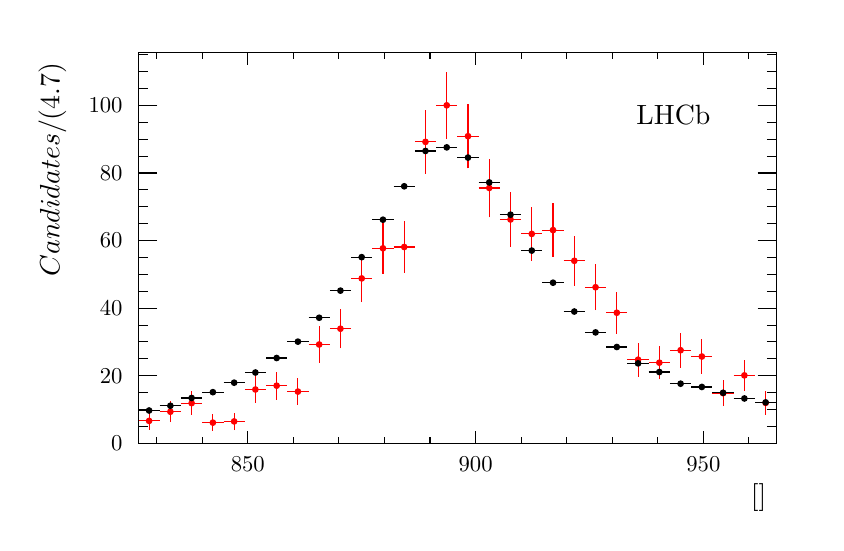
\begin{tikzpicture}
\pgfdeclareplotmark{cross} {
\pgfpathmoveto{\pgfpoint{-0.3\pgfplotmarksize}{\pgfplotmarksize}}
\pgfpathlineto{\pgfpoint{+0.3\pgfplotmarksize}{\pgfplotmarksize}}
\pgfpathlineto{\pgfpoint{+0.3\pgfplotmarksize}{0.3\pgfplotmarksize}}
\pgfpathlineto{\pgfpoint{+1\pgfplotmarksize}{0.3\pgfplotmarksize}}
\pgfpathlineto{\pgfpoint{+1\pgfplotmarksize}{-0.3\pgfplotmarksize}}
\pgfpathlineto{\pgfpoint{+0.3\pgfplotmarksize}{-0.3\pgfplotmarksize}}
\pgfpathlineto{\pgfpoint{+0.3\pgfplotmarksize}{-1.\pgfplotmarksize}}
\pgfpathlineto{\pgfpoint{-0.3\pgfplotmarksize}{-1.\pgfplotmarksize}}
\pgfpathlineto{\pgfpoint{-0.3\pgfplotmarksize}{-0.3\pgfplotmarksize}}
\pgfpathlineto{\pgfpoint{-1.\pgfplotmarksize}{-0.3\pgfplotmarksize}}
\pgfpathlineto{\pgfpoint{-1.\pgfplotmarksize}{0.3\pgfplotmarksize}}
\pgfpathlineto{\pgfpoint{-0.3\pgfplotmarksize}{0.3\pgfplotmarksize}}
\pgfpathclose
\pgfusepathqstroke
}
\pgfdeclareplotmark{cross*} {
\pgfpathmoveto{\pgfpoint{-0.3\pgfplotmarksize}{\pgfplotmarksize}}
\pgfpathlineto{\pgfpoint{+0.3\pgfplotmarksize}{\pgfplotmarksize}}
\pgfpathlineto{\pgfpoint{+0.3\pgfplotmarksize}{0.3\pgfplotmarksize}}
\pgfpathlineto{\pgfpoint{+1\pgfplotmarksize}{0.3\pgfplotmarksize}}
\pgfpathlineto{\pgfpoint{+1\pgfplotmarksize}{-0.3\pgfplotmarksize}}
\pgfpathlineto{\pgfpoint{+0.3\pgfplotmarksize}{-0.3\pgfplotmarksize}}
\pgfpathlineto{\pgfpoint{+0.3\pgfplotmarksize}{-1.\pgfplotmarksize}}
\pgfpathlineto{\pgfpoint{-0.3\pgfplotmarksize}{-1.\pgfplotmarksize}}
\pgfpathlineto{\pgfpoint{-0.3\pgfplotmarksize}{-0.3\pgfplotmarksize}}
\pgfpathlineto{\pgfpoint{-1.\pgfplotmarksize}{-0.3\pgfplotmarksize}}
\pgfpathlineto{\pgfpoint{-1.\pgfplotmarksize}{0.3\pgfplotmarksize}}
\pgfpathlineto{\pgfpoint{-0.3\pgfplotmarksize}{0.3\pgfplotmarksize}}
\pgfpathclose
\pgfusepathqfillstroke
}
\pgfdeclareplotmark{newstar} {
\pgfpathmoveto{\pgfqpoint{0pt}{\pgfplotmarksize}}
\pgfpathlineto{\pgfqpointpolar{44}{0.5\pgfplotmarksize}}
\pgfpathlineto{\pgfqpointpolar{18}{\pgfplotmarksize}}
\pgfpathlineto{\pgfqpointpolar{-20}{0.5\pgfplotmarksize}}
\pgfpathlineto{\pgfqpointpolar{-54}{\pgfplotmarksize}}
\pgfpathlineto{\pgfqpointpolar{-90}{0.5\pgfplotmarksize}}
\pgfpathlineto{\pgfqpointpolar{234}{\pgfplotmarksize}}
\pgfpathlineto{\pgfqpointpolar{198}{0.5\pgfplotmarksize}}
\pgfpathlineto{\pgfqpointpolar{162}{\pgfplotmarksize}}
\pgfpathlineto{\pgfqpointpolar{134}{0.5\pgfplotmarksize}}
\pgfpathclose
\pgfusepathqstroke
}
\pgfdeclareplotmark{newstar*} {
\pgfpathmoveto{\pgfqpoint{0pt}{\pgfplotmarksize}}
\pgfpathlineto{\pgfqpointpolar{44}{0.5\pgfplotmarksize}}
\pgfpathlineto{\pgfqpointpolar{18}{\pgfplotmarksize}}
\pgfpathlineto{\pgfqpointpolar{-20}{0.5\pgfplotmarksize}}
\pgfpathlineto{\pgfqpointpolar{-54}{\pgfplotmarksize}}
\pgfpathlineto{\pgfqpointpolar{-90}{0.5\pgfplotmarksize}}
\pgfpathlineto{\pgfqpointpolar{234}{\pgfplotmarksize}}
\pgfpathlineto{\pgfqpointpolar{198}{0.5\pgfplotmarksize}}
\pgfpathlineto{\pgfqpointpolar{162}{\pgfplotmarksize}}
\pgfpathlineto{\pgfqpointpolar{134}{0.5\pgfplotmarksize}}
\pgfpathclose
\pgfusepathqfillstroke
}
\definecolor{c}{rgb}{1,1,1};
\draw [color=c, fill=c] (0,0) rectangle (10,6.27517);
\draw [color=c, fill=c] (1.4,1.00403) rectangle (9.5,5.96141);
\definecolor{c}{rgb}{0,0,0};
\draw [c] (1.4,1.00403) -- (1.4,5.96141) -- (9.5,5.96141) -- (9.5,1.00403) -- (1.4,1.00403);
\definecolor{c}{rgb}{1,1,1};
\draw [color=c, fill=c] (1.4,1.00403) rectangle (9.5,5.96141);
\definecolor{c}{rgb}{0,0,0};
\draw [c] (1.4,1.00403) -- (1.4,5.96141) -- (9.5,5.96141) -- (9.5,1.00403) -- (1.4,1.00403);
\definecolor{c}{rgb}{1,0,0};
\draw [c,line width=0.4] (1.535,1.17784) -- (1.535,1.28827);
\draw [c,line width=0.4] (1.535,1.28827) -- (1.535,1.39869);
\draw [c,line width=0.4] (1.4,1.28827) -- (1.535,1.28827);
\draw [c,line width=0.4] (1.535,1.28827) -- (1.67,1.28827);
\foreach \P in {(1.535,1.28827)}{\draw[mark options={color=c,fill=c},mark size=2.402402pt,mark=*,mark size=1pt] plot coordinates {\P};}
\draw [c,line width=0.4] (1.805,1.27348) -- (1.805,1.40456);
\draw [c,line width=0.4] (1.805,1.40456) -- (1.805,1.53565);
\draw [c,line width=0.4] (1.67,1.40456) -- (1.805,1.40456);
\draw [c,line width=0.4] (1.805,1.40456) -- (1.94,1.40456);
\foreach \P in {(1.805,1.40456)}{\draw[mark options={color=c,fill=c},mark size=2.402402pt,mark=*,mark size=1pt] plot coordinates {\P};}
\draw [c,line width=0.4] (2.075,1.36594) -- (2.075,1.51382);
\draw [c,line width=0.4] (2.075,1.51382) -- (2.075,1.6617);
\draw [c,line width=0.4] (1.94,1.51382) -- (2.075,1.51382);
\draw [c,line width=0.4] (2.075,1.51382) -- (2.21,1.51382);
\foreach \P in {(2.075,1.51382)}{\draw[mark options={color=c,fill=c},mark size=2.402402pt,mark=*,mark size=1pt] plot coordinates {\P};}
\draw [c,line width=0.4] (2.345,1.16002) -- (2.345,1.26604);
\draw [c,line width=0.4] (2.345,1.26604) -- (2.345,1.37205);
\draw [c,line width=0.4] (2.21,1.26604) -- (2.345,1.26604);
\draw [c,line width=0.4] (2.345,1.26604) -- (2.48,1.26604);
\foreach \P in {(2.345,1.26604)}{\draw[mark options={color=c,fill=c},mark size=2.402402pt,mark=*,mark size=1pt] plot coordinates {\P};}
\draw [c,line width=0.4] (2.615,1.17259) -- (2.615,1.28174);
\draw [c,line width=0.4] (2.615,1.28174) -- (2.615,1.39089);
\draw [c,line width=0.4] (2.48,1.28174) -- (2.615,1.28174);
\draw [c,line width=0.4] (2.615,1.28174) -- (2.75,1.28174);
\foreach \P in {(2.615,1.28174)}{\draw[mark options={color=c,fill=c},mark size=2.402402pt,mark=*,mark size=1pt] plot coordinates {\P};}
\draw [c,line width=0.4] (2.885,1.51579) -- (2.885,1.68695);
\draw [c,line width=0.4] (2.885,1.68695) -- (2.885,1.85811);
\draw [c,line width=0.4] (2.75,1.68695) -- (2.885,1.68695);
\draw [c,line width=0.4] (2.885,1.68695) -- (3.02,1.68695);
\foreach \P in {(2.885,1.68695)}{\draw[mark options={color=c,fill=c},mark size=2.402402pt,mark=*,mark size=1pt] plot coordinates {\P};}
\draw [c,line width=0.4] (3.155,1.55856) -- (3.155,1.73572);
\draw [c,line width=0.4] (3.155,1.73572) -- (3.155,1.91289);
\draw [c,line width=0.4] (3.02,1.73572) -- (3.155,1.73572);
\draw [c,line width=0.4] (3.155,1.73572) -- (3.29,1.73572);
\foreach \P in {(3.155,1.73572)}{\draw[mark options={color=c,fill=c},mark size=2.402402pt,mark=*,mark size=1pt] plot coordinates {\P};}
\draw [c,line width=0.4] (3.425,1.49251) -- (3.425,1.6603);
\draw [c,line width=0.4] (3.425,1.6603) -- (3.425,1.82808);
\draw [c,line width=0.4] (3.29,1.6603) -- (3.425,1.6603);
\draw [c,line width=0.4] (3.425,1.6603) -- (3.56,1.6603);
\foreach \P in {(3.425,1.6603)}{\draw[mark options={color=c,fill=c},mark size=2.402402pt,mark=*,mark size=1pt] plot coordinates {\P};}
\draw [c,line width=0.4] (3.695,2.02663) -- (3.695,2.25862);
\draw [c,line width=0.4] (3.695,2.25862) -- (3.695,2.49061);
\draw [c,line width=0.4] (3.56,2.25862) -- (3.695,2.25862);
\draw [c,line width=0.4] (3.695,2.25862) -- (3.83,2.25862);
\foreach \P in {(3.695,2.25862)}{\draw[mark options={color=c,fill=c},mark size=2.402402pt,mark=*,mark size=1pt] plot coordinates {\P};}
\draw [c,line width=0.4] (3.965,2.209) -- (3.965,2.45881);
\draw [c,line width=0.4] (3.965,2.45881) -- (3.965,2.70862);
\draw [c,line width=0.4] (3.83,2.45881) -- (3.965,2.45881);
\draw [c,line width=0.4] (3.965,2.45881) -- (4.1,2.45881);
\foreach \P in {(3.965,2.45881)}{\draw[mark options={color=c,fill=c},mark size=2.402402pt,mark=*,mark size=1pt] plot coordinates {\P};}
\draw [c,line width=0.4] (4.235,2.79809) -- (4.235,3.09778);
\draw [c,line width=0.4] (4.235,3.09778) -- (4.235,3.39748);
\draw [c,line width=0.4] (4.1,3.09778) -- (4.235,3.09778);
\draw [c,line width=0.4] (4.235,3.09778) -- (4.37,3.09778);
\foreach \P in {(4.235,3.09778)}{\draw[mark options={color=c,fill=c},mark size=2.402402pt,mark=*,mark size=1pt] plot coordinates {\P};}
\draw [c,line width=0.4] (4.505,3.1545) -- (4.505,3.48044);
\draw [c,line width=0.4] (4.505,3.48044) -- (4.505,3.80637);
\draw [c,line width=0.4] (4.37,3.48044) -- (4.505,3.48044);
\draw [c,line width=0.4] (4.505,3.48044) -- (4.64,3.48044);
\foreach \P in {(4.505,3.48044)}{\draw[mark options={color=c,fill=c},mark size=2.402402pt,mark=*,mark size=1pt] plot coordinates {\P};}
\draw [c,line width=0.4] (4.775,3.16967) -- (4.775,3.49667);
\draw [c,line width=0.4] (4.775,3.49667) -- (4.775,3.82366);
\draw [c,line width=0.4] (4.64,3.49667) -- (4.775,3.49667);
\draw [c,line width=0.4] (4.775,3.49667) -- (4.91,3.49667);
\foreach \P in {(4.775,3.49667)}{\draw[mark options={color=c,fill=c},mark size=2.402402pt,mark=*,mark size=1pt] plot coordinates {\P};}
\draw [c,line width=0.4] (5.045,4.42665) -- (5.045,4.83187);
\draw [c,line width=0.4] (5.045,4.83187) -- (5.045,5.23709);
\draw [c,line width=0.4] (4.91,4.83187) -- (5.045,4.83187);
\draw [c,line width=0.4] (5.045,4.83187) -- (5.18,4.83187);
\foreach \P in {(5.045,4.83187)}{\draw[mark options={color=c,fill=c},mark size=2.402402pt,mark=*,mark size=1pt] plot coordinates {\P};}
\draw [c,line width=0.4] (5.315,4.86715) -- (5.315,5.29625);
\draw [c,line width=0.4] (5.315,5.29625) -- (5.315,5.72534);
\draw [c,line width=0.4] (5.18,5.29625) -- (5.315,5.29625);
\draw [c,line width=0.4] (5.315,5.29625) -- (5.45,5.29625);
\foreach \P in {(5.315,5.29625)}{\draw[mark options={color=c,fill=c},mark size=2.402402pt,mark=*,mark size=1pt] plot coordinates {\P};}
\draw [c,line width=0.4] (5.585,4.4952) -- (5.585,4.90423);
\draw [c,line width=0.4] (5.585,4.90423) -- (5.585,5.31327);
\draw [c,line width=0.4] (5.45,4.90423) -- (5.585,4.90423);
\draw [c,line width=0.4] (5.585,4.90423) -- (5.72,4.90423);
\foreach \P in {(5.585,4.90423)}{\draw[mark options={color=c,fill=c},mark size=2.402402pt,mark=*,mark size=1pt] plot coordinates {\P};}
\draw [c,line width=0.4] (5.855,3.87371) -- (5.855,4.24667);
\draw [c,line width=0.4] (5.855,4.24667) -- (5.855,4.61964);
\draw [c,line width=0.4] (5.72,4.24667) -- (5.855,4.24667);
\draw [c,line width=0.4] (5.855,4.24667) -- (5.99,4.24667);
\foreach \P in {(5.855,4.24667)}{\draw[mark options={color=c,fill=c},mark size=2.402402pt,mark=*,mark size=1pt] plot coordinates {\P};}
\draw [c,line width=0.4] (6.125,3.49716) -- (6.125,3.84635);
\draw [c,line width=0.4] (6.125,3.84635) -- (6.125,4.19553);
\draw [c,line width=0.4] (5.99,3.84635) -- (6.125,3.84635);
\draw [c,line width=0.4] (6.125,3.84635) -- (6.26,3.84635);
\foreach \P in {(6.125,3.84635)}{\draw[mark options={color=c,fill=c},mark size=2.402402pt,mark=*,mark size=1pt] plot coordinates {\P};}
\draw [c,line width=0.4] (6.395,3.32518) -- (6.395,3.66291);
\draw [c,line width=0.4] (6.395,3.66291) -- (6.395,4.00064);
\draw [c,line width=0.4] (6.26,3.66291) -- (6.395,3.66291);
\draw [c,line width=0.4] (6.395,3.66291) -- (6.53,3.66291);
\foreach \P in {(6.395,3.66291)}{\draw[mark options={color=c,fill=c},mark size=2.402402pt,mark=*,mark size=1pt] plot coordinates {\P};}
\draw [c,line width=0.4] (6.665,3.37055) -- (6.665,3.71134);
\draw [c,line width=0.4] (6.665,3.71134) -- (6.665,4.05213);
\draw [c,line width=0.4] (6.53,3.71134) -- (6.665,3.71134);
\draw [c,line width=0.4] (6.665,3.71134) -- (6.8,3.71134);
\foreach \P in {(6.665,3.71134)}{\draw[mark options={color=c,fill=c},mark size=2.402402pt,mark=*,mark size=1pt] plot coordinates {\P};}
\draw [c,line width=0.4] (6.935,3.00614) -- (6.935,3.32143);
\draw [c,line width=0.4] (6.935,3.32143) -- (6.935,3.63673);
\draw [c,line width=0.4] (6.8,3.32143) -- (6.935,3.32143);
\draw [c,line width=0.4] (6.935,3.32143) -- (7.07,3.32143);
\foreach \P in {(6.935,3.32143)}{\draw[mark options={color=c,fill=c},mark size=2.402402pt,mark=*,mark size=1pt] plot coordinates {\P};}
\draw [c,line width=0.4] (7.205,2.69423) -- (7.205,2.9858);
\draw [c,line width=0.4] (7.205,2.9858) -- (7.205,3.27737);
\draw [c,line width=0.4] (7.07,2.9858) -- (7.205,2.9858);
\draw [c,line width=0.4] (7.205,2.9858) -- (7.34,2.9858);
\foreach \P in {(7.205,2.9858)}{\draw[mark options={color=c,fill=c},mark size=2.402402pt,mark=*,mark size=1pt] plot coordinates {\P};}
\draw [c,line width=0.4] (7.475,2.39511) -- (7.475,2.66178);
\draw [c,line width=0.4] (7.475,2.66178) -- (7.475,2.92845);
\draw [c,line width=0.4] (7.34,2.66178) -- (7.475,2.66178);
\draw [c,line width=0.4] (7.475,2.66178) -- (7.61,2.66178);
\foreach \P in {(7.475,2.66178)}{\draw[mark options={color=c,fill=c},mark size=2.402402pt,mark=*,mark size=1pt] plot coordinates {\P};}
\draw [c,line width=0.4] (7.745,1.85202) -- (7.745,2.0654);
\draw [c,line width=0.4] (7.745,2.0654) -- (7.745,2.27878);
\draw [c,line width=0.4] (7.61,2.0654) -- (7.745,2.0654);
\draw [c,line width=0.4] (7.745,2.0654) -- (7.88,2.0654);
\foreach \P in {(7.745,2.0654)}{\draw[mark options={color=c,fill=c},mark size=2.402402pt,mark=*,mark size=1pt] plot coordinates {\P};}
\draw [c,line width=0.4] (8.015,1.81816) -- (8.015,2.02772);
\draw [c,line width=0.4] (8.015,2.02772) -- (8.015,2.23728);
\draw [c,line width=0.4] (7.88,2.02772) -- (8.015,2.02772);
\draw [c,line width=0.4] (8.015,2.02772) -- (8.15,2.02772);
\foreach \P in {(8.015,2.02772)}{\draw[mark options={color=c,fill=c},mark size=2.402402pt,mark=*,mark size=1pt] plot coordinates {\P};}
\draw [c,line width=0.4] (8.285,1.96043) -- (8.285,2.18556);
\draw [c,line width=0.4] (8.285,2.18556) -- (8.285,2.4107);
\draw [c,line width=0.4] (8.15,2.18556) -- (8.285,2.18556);
\draw [c,line width=0.4] (8.285,2.18556) -- (8.42,2.18556);
\foreach \P in {(8.285,2.18556)}{\draw[mark options={color=c,fill=c},mark size=2.402402pt,mark=*,mark size=1pt] plot coordinates {\P};}
\draw [c,line width=0.4] (8.555,1.88822) -- (8.555,2.1056);
\draw [c,line width=0.4] (8.555,2.1056) -- (8.555,2.32299);
\draw [c,line width=0.4] (8.42,2.1056) -- (8.555,2.1056);
\draw [c,line width=0.4] (8.555,2.1056) -- (8.69,2.1056);
\foreach \P in {(8.555,2.1056)}{\draw[mark options={color=c,fill=c},mark size=2.402402pt,mark=*,mark size=1pt] plot coordinates {\P};}
\draw [c,line width=0.4] (8.825,1.47523) -- (8.825,1.64046);
\draw [c,line width=0.4] (8.825,1.64046) -- (8.825,1.80569);
\draw [c,line width=0.4] (8.69,1.64046) -- (8.825,1.64046);
\draw [c,line width=0.4] (8.825,1.64046) -- (8.96,1.64046);
\foreach \P in {(8.825,1.64046)}{\draw[mark options={color=c,fill=c},mark size=2.402402pt,mark=*,mark size=1pt] plot coordinates {\P};}
\draw [c,line width=0.4] (9.095,1.67404) -- (9.095,1.86638);
\draw [c,line width=0.4] (9.095,1.86638) -- (9.095,2.05871);
\draw [c,line width=0.4] (8.96,1.86638) -- (9.095,1.86638);
\draw [c,line width=0.4] (9.095,1.86638) -- (9.23,1.86638);
\foreach \P in {(9.095,1.86638)}{\draw[mark options={color=c,fill=c},mark size=2.402402pt,mark=*,mark size=1pt] plot coordinates {\P};}
\draw [c,line width=0.4] (9.365,1.36845) -- (9.365,1.51676);
\draw [c,line width=0.4] (9.365,1.51676) -- (9.365,1.66507);
\draw [c,line width=0.4] (9.23,1.51676) -- (9.365,1.51676);
\draw [c,line width=0.4] (9.365,1.51676) -- (9.5,1.51676);
\foreach \P in {(9.365,1.51676)}{\draw[mark options={color=c,fill=c},mark size=2.402402pt,mark=*,mark size=1pt] plot coordinates {\P};}
\definecolor{c}{rgb}{0,0,0};
\draw [c,line width=0.4] (1.4,1.00403) -- (9.5,1.00403);
\draw [anchor= east] (9.5,0.317272) node[scale=1.00614, rotate=0]{$\mkpi [\mevcc]$};
\draw [c,line width=0.4] (2.78857,1.15651) -- (2.78857,1.00403);
\draw [c,line width=0.4] (3.36714,1.08027) -- (3.36714,1.00403);
\draw [c,line width=0.4] (3.94571,1.08027) -- (3.94571,1.00403);
\draw [c,line width=0.4] (4.52429,1.08027) -- (4.52429,1.00403);
\draw [c,line width=0.4] (5.10286,1.08027) -- (5.10286,1.00403);
\draw [c,line width=0.4] (5.68143,1.15651) -- (5.68143,1.00403);
\draw [c,line width=0.4] (6.26,1.08027) -- (6.26,1.00403);
\draw [c,line width=0.4] (6.83857,1.08027) -- (6.83857,1.00403);
\draw [c,line width=0.4] (7.41714,1.08027) -- (7.41714,1.00403);
\draw [c,line width=0.4] (7.99571,1.08027) -- (7.99571,1.00403);
\draw [c,line width=0.4] (8.57429,1.15651) -- (8.57429,1.00403);
\draw [c,line width=0.4] (2.78857,1.15651) -- (2.78857,1.00403);
\draw [c,line width=0.4] (2.21,1.08027) -- (2.21,1.00403);
\draw [c,line width=0.4] (1.63143,1.08027) -- (1.63143,1.00403);
\draw [c,line width=0.4] (8.57429,1.15651) -- (8.57429,1.00403);
\draw [c,line width=0.4] (9.15286,1.08027) -- (9.15286,1.00403);
\draw [anchor=base] (2.78857,0.640067) node[scale=0.819821, rotate=0]{850};
\draw [anchor=base] (5.68143,0.640067) node[scale=0.819821, rotate=0]{900};
\draw [anchor=base] (8.57429,0.640067) node[scale=0.819821, rotate=0]{950};
\draw [c,line width=0.4] (1.4,5.96141) -- (9.5,5.96141);
\draw [c,line width=0.4] (2.78857,5.80892) -- (2.78857,5.96141);
\draw [c,line width=0.4] (3.36714,5.88517) -- (3.36714,5.96141);
\draw [c,line width=0.4] (3.94571,5.88517) -- (3.94571,5.96141);
\draw [c,line width=0.4] (4.52429,5.88517) -- (4.52429,5.96141);
\draw [c,line width=0.4] (5.10286,5.88517) -- (5.10286,5.96141);
\draw [c,line width=0.4] (5.68143,5.80892) -- (5.68143,5.96141);
\draw [c,line width=0.4] (6.26,5.88517) -- (6.26,5.96141);
\draw [c,line width=0.4] (6.83857,5.88517) -- (6.83857,5.96141);
\draw [c,line width=0.4] (7.41714,5.88517) -- (7.41714,5.96141);
\draw [c,line width=0.4] (7.99571,5.88517) -- (7.99571,5.96141);
\draw [c,line width=0.4] (8.57429,5.80892) -- (8.57429,5.96141);
\draw [c,line width=0.4] (2.78857,5.80892) -- (2.78857,5.96141);
\draw [c,line width=0.4] (2.21,5.88517) -- (2.21,5.96141);
\draw [c,line width=0.4] (1.63143,5.88517) -- (1.63143,5.96141);
\draw [c,line width=0.4] (8.57429,5.80892) -- (8.57429,5.96141);
\draw [c,line width=0.4] (9.15286,5.88517) -- (9.15286,5.96141);
\draw [c,line width=0.4] (1.4,1.00403) -- (1.4,5.96141);
\draw [anchor= east] (0.3056,5.96141) node[scale=1.00614, rotate=90]{$\text{Candidates} / (4.7 \mevcc)$};
\draw [c,line width=0.4] (1.637,1.00403) -- (1.4,1.00403);
\draw [c,line width=0.4] (1.5185,1.21851) -- (1.4,1.21851);
\draw [c,line width=0.4] (1.5185,1.433) -- (1.4,1.433);
\draw [c,line width=0.4] (1.5185,1.64749) -- (1.4,1.64749);
\draw [c,line width=0.4] (1.637,1.86198) -- (1.4,1.86198);
\draw [c,line width=0.4] (1.5185,2.07647) -- (1.4,2.07647);
\draw [c,line width=0.4] (1.5185,2.29095) -- (1.4,2.29095);
\draw [c,line width=0.4] (1.5185,2.50544) -- (1.4,2.50544);
\draw [c,line width=0.4] (1.637,2.71993) -- (1.4,2.71993);
\draw [c,line width=0.4] (1.5185,2.93442) -- (1.4,2.93442);
\draw [c,line width=0.4] (1.5185,3.1489) -- (1.4,3.1489);
\draw [c,line width=0.4] (1.5185,3.36339) -- (1.4,3.36339);
\draw [c,line width=0.4] (1.637,3.57788) -- (1.4,3.57788);
\draw [c,line width=0.4] (1.5185,3.79237) -- (1.4,3.79237);
\draw [c,line width=0.4] (1.5185,4.00686) -- (1.4,4.00686);
\draw [c,line width=0.4] (1.5185,4.22134) -- (1.4,4.22134);
\draw [c,line width=0.4] (1.637,4.43583) -- (1.4,4.43583);
\draw [c,line width=0.4] (1.5185,4.65032) -- (1.4,4.65032);
\draw [c,line width=0.4] (1.5185,4.86481) -- (1.4,4.86481);
\draw [c,line width=0.4] (1.5185,5.07929) -- (1.4,5.07929);
\draw [c,line width=0.4] (1.637,5.29378) -- (1.4,5.29378);
\draw [c,line width=0.4] (1.637,5.29378) -- (1.4,5.29378);
\draw [c,line width=0.4] (1.5185,5.50827) -- (1.4,5.50827);
\draw [c,line width=0.4] (1.5185,5.72276) -- (1.4,5.72276);
\draw [c,line width=0.4] (1.5185,5.93724) -- (1.4,5.93724);
\draw [anchor= east] (1.3,1.00403) node[scale=0.819821, rotate=0]{0};
\draw [anchor= east] (1.3,1.86198) node[scale=0.819821, rotate=0]{20};
\draw [anchor= east] (1.3,2.71993) node[scale=0.819821, rotate=0]{40};
\draw [anchor= east] (1.3,3.57788) node[scale=0.819821, rotate=0]{60};
\draw [anchor= east] (1.3,4.43583) node[scale=0.819821, rotate=0]{80};
\draw [anchor= east] (1.3,5.29378) node[scale=0.819821, rotate=0]{100};
\draw [c,line width=0.4] (9.5,1.00403) -- (9.5,5.96141);
\draw [c,line width=0.4] (9.263,1.00403) -- (9.5,1.00403);
\draw [c,line width=0.4] (9.3815,1.21851) -- (9.5,1.21851);
\draw [c,line width=0.4] (9.3815,1.433) -- (9.5,1.433);
\draw [c,line width=0.4] (9.3815,1.64749) -- (9.5,1.64749);
\draw [c,line width=0.4] (9.263,1.86198) -- (9.5,1.86198);
\draw [c,line width=0.4] (9.3815,2.07647) -- (9.5,2.07647);
\draw [c,line width=0.4] (9.3815,2.29095) -- (9.5,2.29095);
\draw [c,line width=0.4] (9.3815,2.50544) -- (9.5,2.50544);
\draw [c,line width=0.4] (9.263,2.71993) -- (9.5,2.71993);
\draw [c,line width=0.4] (9.3815,2.93442) -- (9.5,2.93442);
\draw [c,line width=0.4] (9.3815,3.1489) -- (9.5,3.1489);
\draw [c,line width=0.4] (9.3815,3.36339) -- (9.5,3.36339);
\draw [c,line width=0.4] (9.263,3.57788) -- (9.5,3.57788);
\draw [c,line width=0.4] (9.3815,3.79237) -- (9.5,3.79237);
\draw [c,line width=0.4] (9.3815,4.00686) -- (9.5,4.00686);
\draw [c,line width=0.4] (9.3815,4.22134) -- (9.5,4.22134);
\draw [c,line width=0.4] (9.263,4.43583) -- (9.5,4.43583);
\draw [c,line width=0.4] (9.3815,4.65032) -- (9.5,4.65032);
\draw [c,line width=0.4] (9.3815,4.86481) -- (9.5,4.86481);
\draw [c,line width=0.4] (9.3815,5.07929) -- (9.5,5.07929);
\draw [c,line width=0.4] (9.263,5.29378) -- (9.5,5.29378);
\draw [c,line width=0.4] (9.263,5.29378) -- (9.5,5.29378);
\draw [c,line width=0.4] (9.3815,5.50827) -- (9.5,5.50827);
\draw [c,line width=0.4] (9.3815,5.72276) -- (9.5,5.72276);
\draw [c,line width=0.4] (9.3815,5.93724) -- (9.5,5.93724);
\draw [c,line width=0.4] (1.535,1.41014) -- (1.535,1.42026);
\draw [c,line width=0.4] (1.535,1.42026) -- (1.535,1.43038);
\draw [c,line width=0.4] (1.4,1.42026) -- (1.535,1.42026);
\draw [c,line width=0.4] (1.535,1.42026) -- (1.67,1.42026);
\foreach \P in {(1.535,1.42026)}{\draw[mark options={color=c,fill=c},mark size=2.402402pt,mark=*,mark size=1pt] plot coordinates {\P};}
\draw [c,line width=0.4] (1.805,1.46974) -- (1.805,1.48057);
\draw [c,line width=0.4] (1.805,1.48057) -- (1.805,1.4914);
\draw [c,line width=0.4] (1.67,1.48057) -- (1.805,1.48057);
\draw [c,line width=0.4] (1.805,1.48057) -- (1.94,1.48057);
\foreach \P in {(1.805,1.48057)}{\draw[mark options={color=c,fill=c},mark size=2.402402pt,mark=*,mark size=1pt] plot coordinates {\P};}
\draw [c,line width=0.4] (2.075,1.56752) -- (2.075,1.57942);
\draw [c,line width=0.4] (2.075,1.57942) -- (2.075,1.59133);
\draw [c,line width=0.4] (1.94,1.57942) -- (2.075,1.57942);
\draw [c,line width=0.4] (2.075,1.57942) -- (2.21,1.57942);
\foreach \P in {(2.075,1.57942)}{\draw[mark options={color=c,fill=c},mark size=2.402402pt,mark=*,mark size=1pt] plot coordinates {\P};}
\draw [c,line width=0.4] (2.345,1.64049) -- (2.345,1.65313);
\draw [c,line width=0.4] (2.345,1.65313) -- (2.345,1.66577);
\draw [c,line width=0.4] (2.21,1.65313) -- (2.345,1.65313);
\draw [c,line width=0.4] (2.345,1.65313) -- (2.48,1.65313);
\foreach \P in {(2.345,1.65313)}{\draw[mark options={color=c,fill=c},mark size=2.402402pt,mark=*,mark size=1pt] plot coordinates {\P};}
\draw [c,line width=0.4] (2.615,1.75977) -- (2.615,1.77354);
\draw [c,line width=0.4] (2.615,1.77354) -- (2.615,1.7873);
\draw [c,line width=0.4] (2.48,1.77354) -- (2.615,1.77354);
\draw [c,line width=0.4] (2.615,1.77354) -- (2.75,1.77354);
\foreach \P in {(2.615,1.77354)}{\draw[mark options={color=c,fill=c},mark size=2.402402pt,mark=*,mark size=1pt] plot coordinates {\P};}
\draw [c,line width=0.4] (2.885,1.88793) -- (2.885,1.9028);
\draw [c,line width=0.4] (2.885,1.9028) -- (2.885,1.91768);
\draw [c,line width=0.4] (2.75,1.9028) -- (2.885,1.9028);
\draw [c,line width=0.4] (2.885,1.9028) -- (3.02,1.9028);
\foreach \P in {(2.885,1.9028)}{\draw[mark options={color=c,fill=c},mark size=2.402402pt,mark=*,mark size=1pt] plot coordinates {\P};}
\draw [c,line width=0.4] (3.155,2.07054) -- (3.155,2.08687);
\draw [c,line width=0.4] (3.155,2.08687) -- (3.155,2.1032);
\draw [c,line width=0.4] (3.02,2.08687) -- (3.155,2.08687);
\draw [c,line width=0.4] (3.155,2.08687) -- (3.29,2.08687);
\foreach \P in {(3.155,2.08687)}{\draw[mark options={color=c,fill=c},mark size=2.402402pt,mark=*,mark size=1pt] plot coordinates {\P};}
\draw [c,line width=0.4] (3.425,2.2771) -- (3.425,2.29493);
\draw [c,line width=0.4] (3.425,2.29493) -- (3.425,2.31276);
\draw [c,line width=0.4] (3.29,2.29493) -- (3.425,2.29493);
\draw [c,line width=0.4] (3.425,2.29493) -- (3.56,2.29493);
\foreach \P in {(3.425,2.29493)}{\draw[mark options={color=c,fill=c},mark size=2.402402pt,mark=*,mark size=1pt] plot coordinates {\P};}
\draw [c,line width=0.4] (3.695,2.57837) -- (3.695,2.59818);
\draw [c,line width=0.4] (3.695,2.59818) -- (3.695,2.618);
\draw [c,line width=0.4] (3.56,2.59818) -- (3.695,2.59818);
\draw [c,line width=0.4] (3.695,2.59818) -- (3.83,2.59818);
\foreach \P in {(3.695,2.59818)}{\draw[mark options={color=c,fill=c},mark size=2.402402pt,mark=*,mark size=1pt] plot coordinates {\P};}
\draw [c,line width=0.4] (3.965,2.92076) -- (3.965,2.94261);
\draw [c,line width=0.4] (3.965,2.94261) -- (3.965,2.96446);
\draw [c,line width=0.4] (3.83,2.94261) -- (3.965,2.94261);
\draw [c,line width=0.4] (3.965,2.94261) -- (4.1,2.94261);
\foreach \P in {(3.965,2.94261)}{\draw[mark options={color=c,fill=c},mark size=2.402402pt,mark=*,mark size=1pt] plot coordinates {\P};}
\draw [c,line width=0.4] (4.235,3.34382) -- (4.235,3.36795);
\draw [c,line width=0.4] (4.235,3.36795) -- (4.235,3.39208);
\draw [c,line width=0.4] (4.1,3.36795) -- (4.235,3.36795);
\draw [c,line width=0.4] (4.235,3.36795) -- (4.37,3.36795);
\foreach \P in {(4.235,3.36795)}{\draw[mark options={color=c,fill=c},mark size=2.402402pt,mark=*,mark size=1pt] plot coordinates {\P};}
\draw [c,line width=0.4] (4.505,3.81695) -- (4.505,3.84339);
\draw [c,line width=0.4] (4.505,3.84339) -- (4.505,3.86984);
\draw [c,line width=0.4] (4.37,3.84339) -- (4.505,3.84339);
\draw [c,line width=0.4] (4.505,3.84339) -- (4.64,3.84339);
\foreach \P in {(4.505,3.84339)}{\draw[mark options={color=c,fill=c},mark size=2.402402pt,mark=*,mark size=1pt] plot coordinates {\P};}
\draw [c,line width=0.4] (4.775,4.23942) -- (4.775,4.26777);
\draw [c,line width=0.4] (4.775,4.26777) -- (4.775,4.29612);
\draw [c,line width=0.4] (4.64,4.26777) -- (4.775,4.26777);
\draw [c,line width=0.4] (4.775,4.26777) -- (4.91,4.26777);
\foreach \P in {(4.775,4.26777)}{\draw[mark options={color=c,fill=c},mark size=2.402402pt,mark=*,mark size=1pt] plot coordinates {\P};}
\draw [c,line width=0.4] (5.045,4.68612) -- (5.045,4.71636);
\draw [c,line width=0.4] (5.045,4.71636) -- (5.045,4.7466);
\draw [c,line width=0.4] (4.91,4.71636) -- (5.045,4.71636);
\draw [c,line width=0.4] (5.045,4.71636) -- (5.18,4.71636);
\foreach \P in {(5.045,4.71636)}{\draw[mark options={color=c,fill=c},mark size=2.402402pt,mark=*,mark size=1pt] plot coordinates {\P};}
\draw [c,line width=0.4] (5.315,4.73167) -- (5.315,4.76209);
\draw [c,line width=0.4] (5.315,4.76209) -- (5.315,4.79251);
\draw [c,line width=0.4] (5.18,4.76209) -- (5.315,4.76209);
\draw [c,line width=0.4] (5.315,4.76209) -- (5.45,4.76209);
\foreach \P in {(5.315,4.76209)}{\draw[mark options={color=c,fill=c},mark size=2.402402pt,mark=*,mark size=1pt] plot coordinates {\P};}
\draw [c,line width=0.4] (5.585,4.60254) -- (5.585,4.63244);
\draw [c,line width=0.4] (5.585,4.63244) -- (5.585,4.66233);
\draw [c,line width=0.4] (5.45,4.63244) -- (5.585,4.63244);
\draw [c,line width=0.4] (5.585,4.63244) -- (5.72,4.63244);
\foreach \P in {(5.585,4.63244)}{\draw[mark options={color=c,fill=c},mark size=2.402402pt,mark=*,mark size=1pt] plot coordinates {\P};}
\draw [c,line width=0.4] (5.855,4.28818) -- (5.855,4.31675);
\draw [c,line width=0.4] (5.855,4.31675) -- (5.855,4.34531);
\draw [c,line width=0.4] (5.72,4.31675) -- (5.855,4.31675);
\draw [c,line width=0.4] (5.855,4.31675) -- (5.99,4.31675);
\foreach \P in {(5.855,4.31675)}{\draw[mark options={color=c,fill=c},mark size=2.402402pt,mark=*,mark size=1pt] plot coordinates {\P};}
\draw [c,line width=0.4] (6.125,3.88034) -- (6.125,3.90708);
\draw [c,line width=0.4] (6.125,3.90708) -- (6.125,3.93382);
\draw [c,line width=0.4] (5.99,3.90708) -- (6.125,3.90708);
\draw [c,line width=0.4] (6.125,3.90708) -- (6.26,3.90708);
\foreach \P in {(6.125,3.90708)}{\draw[mark options={color=c,fill=c},mark size=2.402402pt,mark=*,mark size=1pt] plot coordinates {\P};}
\draw [c,line width=0.4] (6.395,3.42666) -- (6.395,3.45121);
\draw [c,line width=0.4] (6.395,3.45121) -- (6.395,3.47576);
\draw [c,line width=0.4] (6.26,3.45121) -- (6.395,3.45121);
\draw [c,line width=0.4] (6.395,3.45121) -- (6.53,3.45121);
\foreach \P in {(6.395,3.45121)}{\draw[mark options={color=c,fill=c},mark size=2.402402pt,mark=*,mark size=1pt] plot coordinates {\P};}
\draw [c,line width=0.4] (6.665,3.02074) -- (6.665,3.04315);
\draw [c,line width=0.4] (6.665,3.04315) -- (6.665,3.06556);
\draw [c,line width=0.4] (6.53,3.04315) -- (6.665,3.04315);
\draw [c,line width=0.4] (6.665,3.04315) -- (6.8,3.04315);
\foreach \P in {(6.665,3.04315)}{\draw[mark options={color=c,fill=c},mark size=2.402402pt,mark=*,mark size=1pt] plot coordinates {\P};}
\draw [c,line width=0.4] (6.935,2.65694) -- (6.935,2.67724);
\draw [c,line width=0.4] (6.935,2.67724) -- (6.935,2.69754);
\draw [c,line width=0.4] (6.8,2.67724) -- (6.935,2.67724);
\draw [c,line width=0.4] (6.935,2.67724) -- (7.07,2.67724);
\foreach \P in {(6.935,2.67724)}{\draw[mark options={color=c,fill=c},mark size=2.402402pt,mark=*,mark size=1pt] plot coordinates {\P};}
\draw [c,line width=0.4] (7.205,2.39361) -- (7.205,2.41223);
\draw [c,line width=0.4] (7.205,2.41223) -- (7.205,2.43086);
\draw [c,line width=0.4] (7.07,2.41223) -- (7.205,2.41223);
\draw [c,line width=0.4] (7.205,2.41223) -- (7.34,2.41223);
\foreach \P in {(7.205,2.41223)}{\draw[mark options={color=c,fill=c},mark size=2.402402pt,mark=*,mark size=1pt] plot coordinates {\P};}
\draw [c,line width=0.4] (7.475,2.20922) -- (7.475,2.22657);
\draw [c,line width=0.4] (7.475,2.22657) -- (7.475,2.24392);
\draw [c,line width=0.4] (7.34,2.22657) -- (7.475,2.22657);
\draw [c,line width=0.4] (7.475,2.22657) -- (7.61,2.22657);
\foreach \P in {(7.475,2.22657)}{\draw[mark options={color=c,fill=c},mark size=2.402402pt,mark=*,mark size=1pt] plot coordinates {\P};}
\draw [c,line width=0.4] (7.745,2.00304) -- (7.745,2.01885);
\draw [c,line width=0.4] (7.745,2.01885) -- (7.745,2.03466);
\draw [c,line width=0.4] (7.61,2.01885) -- (7.745,2.01885);
\draw [c,line width=0.4] (7.745,2.01885) -- (7.88,2.01885);
\foreach \P in {(7.745,2.01885)}{\draw[mark options={color=c,fill=c},mark size=2.402402pt,mark=*,mark size=1pt] plot coordinates {\P};}
\draw [c,line width=0.4] (8.015,1.89412) -- (8.015,1.90905);
\draw [c,line width=0.4] (8.015,1.90905) -- (8.015,1.92398);
\draw [c,line width=0.4] (7.88,1.90905) -- (8.015,1.90905);
\draw [c,line width=0.4] (8.015,1.90905) -- (8.15,1.90905);
\foreach \P in {(8.015,1.90905)}{\draw[mark options={color=c,fill=c},mark size=2.402402pt,mark=*,mark size=1pt] plot coordinates {\P};}
\draw [c,line width=0.4] (8.285,1.74702) -- (8.285,1.76067);
\draw [c,line width=0.4] (8.285,1.76067) -- (8.285,1.77432);
\draw [c,line width=0.4] (8.15,1.76067) -- (8.285,1.76067);
\draw [c,line width=0.4] (8.285,1.76067) -- (8.42,1.76067);
\foreach \P in {(8.285,1.76067)}{\draw[mark options={color=c,fill=c},mark size=2.402402pt,mark=*,mark size=1pt] plot coordinates {\P};}
\draw [c,line width=0.4] (8.555,1.70609) -- (8.555,1.71936);
\draw [c,line width=0.4] (8.555,1.71936) -- (8.555,1.73263);
\draw [c,line width=0.4] (8.42,1.71936) -- (8.555,1.71936);
\draw [c,line width=0.4] (8.555,1.71936) -- (8.69,1.71936);
\foreach \P in {(8.555,1.71936)}{\draw[mark options={color=c,fill=c},mark size=2.402402pt,mark=*,mark size=1pt] plot coordinates {\P};}
\draw [c,line width=0.4] (8.825,1.63255) -- (8.825,1.64512);
\draw [c,line width=0.4] (8.825,1.64512) -- (8.825,1.65768);
\draw [c,line width=0.4] (8.69,1.64512) -- (8.825,1.64512);
\draw [c,line width=0.4] (8.825,1.64512) -- (8.96,1.64512);
\foreach \P in {(8.825,1.64512)}{\draw[mark options={color=c,fill=c},mark size=2.402402pt,mark=*,mark size=1pt] plot coordinates {\P};}
\draw [c,line width=0.4] (9.095,1.56134) -- (9.095,1.57318);
\draw [c,line width=0.4] (9.095,1.57318) -- (9.095,1.58502);
\draw [c,line width=0.4] (8.96,1.57318) -- (9.095,1.57318);
\draw [c,line width=0.4] (9.095,1.57318) -- (9.23,1.57318);
\foreach \P in {(9.095,1.57318)}{\draw[mark options={color=c,fill=c},mark size=2.402402pt,mark=*,mark size=1pt] plot coordinates {\P};}
\draw [c,line width=0.4] (9.365,1.51213) -- (9.365,1.52344);
\draw [c,line width=0.4] (9.365,1.52344) -- (9.365,1.53475);
\draw [c,line width=0.4] (9.23,1.52344) -- (9.365,1.52344);
\draw [c,line width=0.4] (9.365,1.52344) -- (9.5,1.52344);
\foreach \P in {(9.365,1.52344)}{\draw[mark options={color=c,fill=c},mark size=2.402402pt,mark=*,mark size=1pt] plot coordinates {\P};}
\draw [anchor= west] (7.6,5.17701) node[scale=1.00614, rotate=0]{LHCb};
\end{tikzpicture}
}
    \caption{}
    \label{mkpiPlot_raw}
  \end{subfigure}%
  \hfill%
  \begin{subfigure}{0.5\textwidth}
    \raggedleft
    \tikzsetnextfilename{eff_corrected_eff_mdau2}
    \scalebox{0.56}{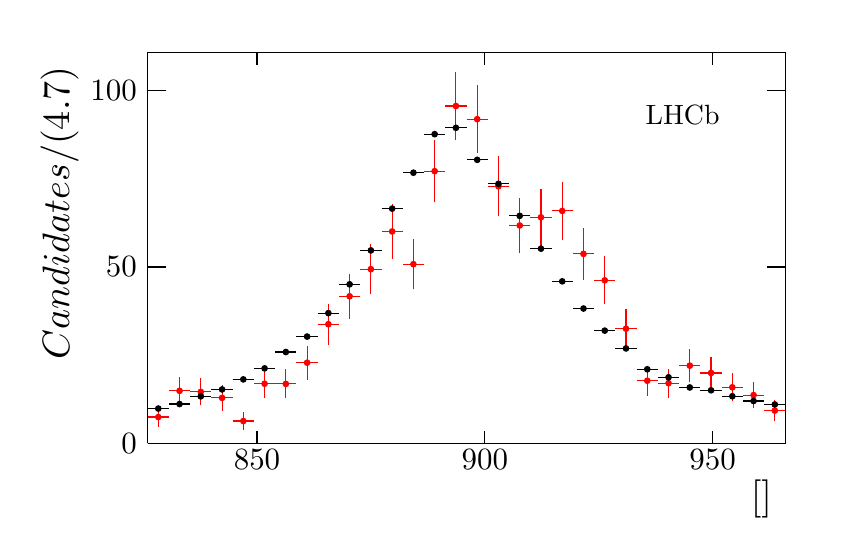
\begin{tikzpicture}
\pgfdeclareplotmark{cross} {
\pgfpathmoveto{\pgfpoint{-0.3\pgfplotmarksize}{\pgfplotmarksize}}
\pgfpathlineto{\pgfpoint{+0.3\pgfplotmarksize}{\pgfplotmarksize}}
\pgfpathlineto{\pgfpoint{+0.3\pgfplotmarksize}{0.3\pgfplotmarksize}}
\pgfpathlineto{\pgfpoint{+1\pgfplotmarksize}{0.3\pgfplotmarksize}}
\pgfpathlineto{\pgfpoint{+1\pgfplotmarksize}{-0.3\pgfplotmarksize}}
\pgfpathlineto{\pgfpoint{+0.3\pgfplotmarksize}{-0.3\pgfplotmarksize}}
\pgfpathlineto{\pgfpoint{+0.3\pgfplotmarksize}{-1.\pgfplotmarksize}}
\pgfpathlineto{\pgfpoint{-0.3\pgfplotmarksize}{-1.\pgfplotmarksize}}
\pgfpathlineto{\pgfpoint{-0.3\pgfplotmarksize}{-0.3\pgfplotmarksize}}
\pgfpathlineto{\pgfpoint{-1.\pgfplotmarksize}{-0.3\pgfplotmarksize}}
\pgfpathlineto{\pgfpoint{-1.\pgfplotmarksize}{0.3\pgfplotmarksize}}
\pgfpathlineto{\pgfpoint{-0.3\pgfplotmarksize}{0.3\pgfplotmarksize}}
\pgfpathclose
\pgfusepathqstroke
}
\pgfdeclareplotmark{cross*} {
\pgfpathmoveto{\pgfpoint{-0.3\pgfplotmarksize}{\pgfplotmarksize}}
\pgfpathlineto{\pgfpoint{+0.3\pgfplotmarksize}{\pgfplotmarksize}}
\pgfpathlineto{\pgfpoint{+0.3\pgfplotmarksize}{0.3\pgfplotmarksize}}
\pgfpathlineto{\pgfpoint{+1\pgfplotmarksize}{0.3\pgfplotmarksize}}
\pgfpathlineto{\pgfpoint{+1\pgfplotmarksize}{-0.3\pgfplotmarksize}}
\pgfpathlineto{\pgfpoint{+0.3\pgfplotmarksize}{-0.3\pgfplotmarksize}}
\pgfpathlineto{\pgfpoint{+0.3\pgfplotmarksize}{-1.\pgfplotmarksize}}
\pgfpathlineto{\pgfpoint{-0.3\pgfplotmarksize}{-1.\pgfplotmarksize}}
\pgfpathlineto{\pgfpoint{-0.3\pgfplotmarksize}{-0.3\pgfplotmarksize}}
\pgfpathlineto{\pgfpoint{-1.\pgfplotmarksize}{-0.3\pgfplotmarksize}}
\pgfpathlineto{\pgfpoint{-1.\pgfplotmarksize}{0.3\pgfplotmarksize}}
\pgfpathlineto{\pgfpoint{-0.3\pgfplotmarksize}{0.3\pgfplotmarksize}}
\pgfpathclose
\pgfusepathqfillstroke
}
\pgfdeclareplotmark{newstar} {
\pgfpathmoveto{\pgfqpoint{0pt}{\pgfplotmarksize}}
\pgfpathlineto{\pgfqpointpolar{44}{0.5\pgfplotmarksize}}
\pgfpathlineto{\pgfqpointpolar{18}{\pgfplotmarksize}}
\pgfpathlineto{\pgfqpointpolar{-20}{0.5\pgfplotmarksize}}
\pgfpathlineto{\pgfqpointpolar{-54}{\pgfplotmarksize}}
\pgfpathlineto{\pgfqpointpolar{-90}{0.5\pgfplotmarksize}}
\pgfpathlineto{\pgfqpointpolar{234}{\pgfplotmarksize}}
\pgfpathlineto{\pgfqpointpolar{198}{0.5\pgfplotmarksize}}
\pgfpathlineto{\pgfqpointpolar{162}{\pgfplotmarksize}}
\pgfpathlineto{\pgfqpointpolar{134}{0.5\pgfplotmarksize}}
\pgfpathclose
\pgfusepathqstroke
}
\pgfdeclareplotmark{newstar*} {
\pgfpathmoveto{\pgfqpoint{0pt}{\pgfplotmarksize}}
\pgfpathlineto{\pgfqpointpolar{44}{0.5\pgfplotmarksize}}
\pgfpathlineto{\pgfqpointpolar{18}{\pgfplotmarksize}}
\pgfpathlineto{\pgfqpointpolar{-20}{0.5\pgfplotmarksize}}
\pgfpathlineto{\pgfqpointpolar{-54}{\pgfplotmarksize}}
\pgfpathlineto{\pgfqpointpolar{-90}{0.5\pgfplotmarksize}}
\pgfpathlineto{\pgfqpointpolar{234}{\pgfplotmarksize}}
\pgfpathlineto{\pgfqpointpolar{198}{0.5\pgfplotmarksize}}
\pgfpathlineto{\pgfqpointpolar{162}{\pgfplotmarksize}}
\pgfpathlineto{\pgfqpointpolar{134}{0.5\pgfplotmarksize}}
\pgfpathclose
\pgfusepathqfillstroke
}
\definecolor{c}{rgb}{1,1,1};
\draw [color=c, fill=c] (0,0) rectangle (10,6.27517);
\draw [color=c, fill=c] (1.4,1.00403) rectangle (9.5,5.96141);
\definecolor{c}{rgb}{0,0,0};
\draw [c] (1.4,1.00403) -- (1.4,5.96141) -- (9.5,5.96141) -- (9.5,1.00403) -- (1.4,1.00403);
\definecolor{c}{rgb}{1,1,1};
\draw [color=c, fill=c] (1.4,1.00403) rectangle (9.5,5.96141);
\definecolor{c}{rgb}{0,0,0};
\draw [c] (1.4,1.00403) -- (1.4,5.96141) -- (9.5,5.96141) -- (9.5,1.00403) -- (1.4,1.00403);
\definecolor{c}{rgb}{1,0,0};
\draw [c,line width=0.4] (1.535,1.21521) -- (1.535,1.33737);
\draw [c,line width=0.4] (1.535,1.33737) -- (1.535,1.45953);
\draw [c,line width=0.4] (1.4,1.33737) -- (1.535,1.33737);
\draw [c,line width=0.4] (1.535,1.33737) -- (1.67,1.33737);
\foreach \P in {(1.535,1.33737)}{\draw[mark options={color=c,fill=c},mark size=2.402402pt,mark=*,mark size=1pt] plot coordinates {\P};}
\draw [c,line width=0.4] (1.805,1.49722) -- (1.805,1.66987);
\draw [c,line width=0.4] (1.805,1.66987) -- (1.805,1.84252);
\draw [c,line width=0.4] (1.67,1.66987) -- (1.805,1.66987);
\draw [c,line width=0.4] (1.805,1.66987) -- (1.94,1.66987);
\foreach \P in {(1.805,1.66987)}{\draw[mark options={color=c,fill=c},mark size=2.402402pt,mark=*,mark size=1pt] plot coordinates {\P};}
\draw [c,line width=0.4] (2.075,1.48566) -- (2.075,1.65658);
\draw [c,line width=0.4] (2.075,1.65658) -- (2.075,1.82749);
\draw [c,line width=0.4] (1.94,1.65658) -- (2.075,1.65658);
\draw [c,line width=0.4] (2.075,1.65658) -- (2.21,1.65658);
\foreach \P in {(2.075,1.65658)}{\draw[mark options={color=c,fill=c},mark size=2.402402pt,mark=*,mark size=1pt] plot coordinates {\P};}
\draw [c,line width=0.4] (2.345,1.41972) -- (2.345,1.58035);
\draw [c,line width=0.4] (2.345,1.58035) -- (2.345,1.74097);
\draw [c,line width=0.4] (2.21,1.58035) -- (2.345,1.58035);
\draw [c,line width=0.4] (2.345,1.58035) -- (2.48,1.58035);
\foreach \P in {(2.345,1.58035)}{\draw[mark options={color=c,fill=c},mark size=2.402402pt,mark=*,mark size=1pt] plot coordinates {\P};}
\draw [c,line width=0.4] (2.615,1.17396) -- (2.615,1.2864);
\draw [c,line width=0.4] (2.615,1.2864) -- (2.615,1.39883);
\draw [c,line width=0.4] (2.48,1.2864) -- (2.615,1.2864);
\draw [c,line width=0.4] (2.615,1.2864) -- (2.75,1.2864);
\foreach \P in {(2.615,1.2864)}{\draw[mark options={color=c,fill=c},mark size=2.402402pt,mark=*,mark size=1pt] plot coordinates {\P};}
\draw [c,line width=0.4] (2.885,1.57625) -- (2.885,1.76025);
\draw [c,line width=0.4] (2.885,1.76025) -- (2.885,1.94424);
\draw [c,line width=0.4] (2.75,1.76025) -- (2.885,1.76025);
\draw [c,line width=0.4] (2.885,1.76025) -- (3.02,1.76025);
\foreach \P in {(2.885,1.76025)}{\draw[mark options={color=c,fill=c},mark size=2.402402pt,mark=*,mark size=1pt] plot coordinates {\P};}
\draw [c,line width=0.4] (3.155,1.57448) -- (3.155,1.75823);
\draw [c,line width=0.4] (3.155,1.75823) -- (3.155,1.94198);
\draw [c,line width=0.4] (3.02,1.75823) -- (3.155,1.75823);
\draw [c,line width=0.4] (3.155,1.75823) -- (3.29,1.75823);
\foreach \P in {(3.155,1.75823)}{\draw[mark options={color=c,fill=c},mark size=2.402402pt,mark=*,mark size=1pt] plot coordinates {\P};}
\draw [c,line width=0.4] (3.425,1.81321) -- (3.425,2.02724);
\draw [c,line width=0.4] (3.425,2.02724) -- (3.425,2.24126);
\draw [c,line width=0.4] (3.29,2.02724) -- (3.425,2.02724);
\draw [c,line width=0.4] (3.425,2.02724) -- (3.56,2.02724);
\foreach \P in {(3.425,2.02724)}{\draw[mark options={color=c,fill=c},mark size=2.402402pt,mark=*,mark size=1pt] plot coordinates {\P};}
\draw [c,line width=0.4] (3.695,2.25571) -- (3.695,2.51587);
\draw [c,line width=0.4] (3.695,2.51587) -- (3.695,2.77603);
\draw [c,line width=0.4] (3.56,2.51587) -- (3.695,2.51587);
\draw [c,line width=0.4] (3.695,2.51587) -- (3.83,2.51587);
\foreach \P in {(3.695,2.51587)}{\draw[mark options={color=c,fill=c},mark size=2.402402pt,mark=*,mark size=1pt] plot coordinates {\P};}
\draw [c,line width=0.4] (3.965,2.58184) -- (3.965,2.87094);
\draw [c,line width=0.4] (3.965,2.87094) -- (3.965,3.16004);
\draw [c,line width=0.4] (3.83,2.87094) -- (3.965,2.87094);
\draw [c,line width=0.4] (3.965,2.87094) -- (4.1,2.87094);
\foreach \P in {(3.965,2.87094)}{\draw[mark options={color=c,fill=c},mark size=2.402402pt,mark=*,mark size=1pt] plot coordinates {\P};}
\draw [c,line width=0.4] (4.235,2.90073) -- (4.235,3.21536);
\draw [c,line width=0.4] (4.235,3.21536) -- (4.235,3.53);
\draw [c,line width=0.4] (4.1,3.21536) -- (4.235,3.21536);
\draw [c,line width=0.4] (4.235,3.21536) -- (4.37,3.21536);
\foreach \P in {(4.235,3.21536)}{\draw[mark options={color=c,fill=c},mark size=2.402402pt,mark=*,mark size=1pt] plot coordinates {\P};}
\draw [c,line width=0.4] (4.505,3.34704) -- (4.505,3.69406);
\draw [c,line width=0.4] (4.505,3.69406) -- (4.505,4.04109);
\draw [c,line width=0.4] (4.37,3.69406) -- (4.505,3.69406);
\draw [c,line width=0.4] (4.505,3.69406) -- (4.64,3.69406);
\foreach \P in {(4.505,3.69406)}{\draw[mark options={color=c,fill=c},mark size=2.402402pt,mark=*,mark size=1pt] plot coordinates {\P};}
\draw [c,line width=0.4] (4.775,2.95942) -- (4.775,3.27852);
\draw [c,line width=0.4] (4.775,3.27852) -- (4.775,3.59762);
\draw [c,line width=0.4] (4.64,3.27852) -- (4.775,3.27852);
\draw [c,line width=0.4] (4.775,3.27852) -- (4.91,3.27852);
\foreach \P in {(4.775,3.27852)}{\draw[mark options={color=c,fill=c},mark size=2.402402pt,mark=*,mark size=1pt] plot coordinates {\P};}
\draw [c,line width=0.4] (5.045,4.06677) -- (5.045,4.46011);
\draw [c,line width=0.4] (5.045,4.46011) -- (5.045,4.85346);
\draw [c,line width=0.4] (4.91,4.46011) -- (5.045,4.46011);
\draw [c,line width=0.4] (5.045,4.46011) -- (5.18,4.46011);
\foreach \P in {(5.045,4.46011)}{\draw[mark options={color=c,fill=c},mark size=2.402402pt,mark=*,mark size=1pt] plot coordinates {\P};}
\draw [c,line width=0.4] (5.315,4.84954) -- (5.315,5.28744);
\draw [c,line width=0.4] (5.315,5.28744) -- (5.315,5.72534);
\draw [c,line width=0.4] (5.18,5.28744) -- (5.315,5.28744);
\draw [c,line width=0.4] (5.315,5.28744) -- (5.45,5.28744);
\foreach \P in {(5.315,5.28744)}{\draw[mark options={color=c,fill=c},mark size=2.402402pt,mark=*,mark size=1pt] plot coordinates {\P};}
\draw [c,line width=0.4] (5.585,4.6908) -- (5.585,5.12006);
\draw [c,line width=0.4] (5.585,5.12006) -- (5.585,5.54932);
\draw [c,line width=0.4] (5.45,5.12006) -- (5.585,5.12006);
\draw [c,line width=0.4] (5.585,5.12006) -- (5.72,5.12006);
\foreach \P in {(5.585,5.12006)}{\draw[mark options={color=c,fill=c},mark size=2.402402pt,mark=*,mark size=1pt] plot coordinates {\P};}
\draw [c,line width=0.4] (5.855,3.88595) -- (5.855,4.26822);
\draw [c,line width=0.4] (5.855,4.26822) -- (5.855,4.65049);
\draw [c,line width=0.4] (5.72,4.26822) -- (5.855,4.26822);
\draw [c,line width=0.4] (5.855,4.26822) -- (5.99,4.26822);
\foreach \P in {(5.855,4.26822)}{\draw[mark options={color=c,fill=c},mark size=2.402402pt,mark=*,mark size=1pt] plot coordinates {\P};}
\draw [c,line width=0.4] (6.125,3.41805) -- (6.125,3.76993);
\draw [c,line width=0.4] (6.125,3.76993) -- (6.125,4.12182);
\draw [c,line width=0.4] (5.99,3.76993) -- (6.125,3.76993);
\draw [c,line width=0.4] (6.125,3.76993) -- (6.26,3.76993);
\foreach \P in {(6.125,3.76993)}{\draw[mark options={color=c,fill=c},mark size=2.402402pt,mark=*,mark size=1pt] plot coordinates {\P};}
\draw [c,line width=0.4] (6.395,3.51549) -- (6.395,3.87393);
\draw [c,line width=0.4] (6.395,3.87393) -- (6.395,4.23237);
\draw [c,line width=0.4] (6.26,3.87393) -- (6.395,3.87393);
\draw [c,line width=0.4] (6.395,3.87393) -- (6.53,3.87393);
\foreach \P in {(6.395,3.87393)}{\draw[mark options={color=c,fill=c},mark size=2.402402pt,mark=*,mark size=1pt] plot coordinates {\P};}
\draw [c,line width=0.4] (6.665,3.5914) -- (6.665,3.95486);
\draw [c,line width=0.4] (6.665,3.95486) -- (6.665,4.31832);
\draw [c,line width=0.4] (6.53,3.95486) -- (6.665,3.95486);
\draw [c,line width=0.4] (6.665,3.95486) -- (6.8,3.95486);
\foreach \P in {(6.665,3.95486)}{\draw[mark options={color=c,fill=c},mark size=2.402402pt,mark=*,mark size=1pt] plot coordinates {\P};}
\draw [c,line width=0.4] (6.935,3.08114) -- (6.935,3.40928);
\draw [c,line width=0.4] (6.935,3.40928) -- (6.935,3.73743);
\draw [c,line width=0.4] (6.8,3.40928) -- (6.935,3.40928);
\draw [c,line width=0.4] (6.935,3.40928) -- (7.07,3.40928);
\foreach \P in {(6.935,3.40928)}{\draw[mark options={color=c,fill=c},mark size=2.402402pt,mark=*,mark size=1pt] plot coordinates {\P};}
\draw [c,line width=0.4] (7.205,2.76932) -- (7.205,3.07371);
\draw [c,line width=0.4] (7.205,3.07371) -- (7.205,3.3781);
\draw [c,line width=0.4] (7.07,3.07371) -- (7.205,3.07371);
\draw [c,line width=0.4] (7.205,3.07371) -- (7.34,3.07371);
\foreach \P in {(7.205,3.07371)}{\draw[mark options={color=c,fill=c},mark size=2.402402pt,mark=*,mark size=1pt] plot coordinates {\P};}
\draw [c,line width=0.4] (7.475,2.2037) -- (7.475,2.45891);
\draw [c,line width=0.4] (7.475,2.45891) -- (7.475,2.71412);
\draw [c,line width=0.4] (7.34,2.45891) -- (7.475,2.45891);
\draw [c,line width=0.4] (7.475,2.45891) -- (7.61,2.45891);
\foreach \P in {(7.475,2.45891)}{\draw[mark options={color=c,fill=c},mark size=2.402402pt,mark=*,mark size=1pt] plot coordinates {\P};}
\draw [c,line width=0.4] (7.745,1.60969) -- (7.745,1.79825);
\draw [c,line width=0.4] (7.745,1.79825) -- (7.745,1.98681);
\draw [c,line width=0.4] (7.61,1.79825) -- (7.745,1.79825);
\draw [c,line width=0.4] (7.745,1.79825) -- (7.88,1.79825);
\foreach \P in {(7.745,1.79825)}{\draw[mark options={color=c,fill=c},mark size=2.402402pt,mark=*,mark size=1pt] plot coordinates {\P};}
\draw [c,line width=0.4] (8.015,1.58243) -- (8.015,1.76728);
\draw [c,line width=0.4] (8.015,1.76728) -- (8.015,1.95213);
\draw [c,line width=0.4] (7.88,1.76728) -- (8.015,1.76728);
\draw [c,line width=0.4] (8.015,1.76728) -- (8.15,1.76728);
\foreach \P in {(8.015,1.76728)}{\draw[mark options={color=c,fill=c},mark size=2.402402pt,mark=*,mark size=1pt] plot coordinates {\P};}
\draw [c,line width=0.4] (8.285,1.7799) -- (8.285,1.99);
\draw [c,line width=0.4] (8.285,1.99) -- (8.285,2.20009);
\draw [c,line width=0.4] (8.15,1.99) -- (8.285,1.99);
\draw [c,line width=0.4] (8.285,1.99) -- (8.42,1.99);
\foreach \P in {(8.285,1.99)}{\draw[mark options={color=c,fill=c},mark size=2.402402pt,mark=*,mark size=1pt] plot coordinates {\P};}
\draw [c,line width=0.4] (8.555,1.69713) -- (8.555,1.89708);
\draw [c,line width=0.4] (8.555,1.89708) -- (8.555,2.09703);
\draw [c,line width=0.4] (8.42,1.89708) -- (8.555,1.89708);
\draw [c,line width=0.4] (8.555,1.89708) -- (8.69,1.89708);
\foreach \P in {(8.555,1.89708)}{\draw[mark options={color=c,fill=c},mark size=2.402402pt,mark=*,mark size=1pt] plot coordinates {\P};}
\draw [c,line width=0.4] (8.825,1.53677) -- (8.825,1.7152);
\draw [c,line width=0.4] (8.825,1.7152) -- (8.825,1.89363);
\draw [c,line width=0.4] (8.69,1.7152) -- (8.825,1.7152);
\draw [c,line width=0.4] (8.825,1.7152) -- (8.96,1.7152);
\foreach \P in {(8.825,1.7152)}{\draw[mark options={color=c,fill=c},mark size=2.402402pt,mark=*,mark size=1pt] plot coordinates {\P};}
\draw [c,line width=0.4] (9.095,1.45023) -- (9.095,1.61571);
\draw [c,line width=0.4] (9.095,1.61571) -- (9.095,1.78118);
\draw [c,line width=0.4] (8.96,1.61571) -- (9.095,1.61571);
\draw [c,line width=0.4] (9.095,1.61571) -- (9.23,1.61571);
\foreach \P in {(9.095,1.61571)}{\draw[mark options={color=c,fill=c},mark size=2.402402pt,mark=*,mark size=1pt] plot coordinates {\P};}
\draw [c,line width=0.4] (9.365,1.28266) -- (9.365,1.41895);
\draw [c,line width=0.4] (9.365,1.41895) -- (9.365,1.55524);
\draw [c,line width=0.4] (9.23,1.41895) -- (9.365,1.41895);
\draw [c,line width=0.4] (9.365,1.41895) -- (9.5,1.41895);
\foreach \P in {(9.365,1.41895)}{\draw[mark options={color=c,fill=c},mark size=2.402402pt,mark=*,mark size=1pt] plot coordinates {\P};}
\definecolor{c}{rgb}{0,0,0};
\draw [c,line width=0.4] (1.4,1.00403) -- (9.5,1.00403);
\draw [anchor= east] (9.5,0.301208) node[scale=1.37879, rotate=0]{$\mkpi [\mevcc]$};
\draw [c,line width=0.4] (2.78857,1.15651) -- (2.78857,1.00403);
\draw [c,line width=0.4] (5.68143,1.15651) -- (5.68143,1.00403);
\draw [c,line width=0.4] (8.57429,1.15651) -- (8.57429,1.00403);
\draw [c,line width=0.4] (2.78857,1.15651) -- (2.78857,1.00403);
\draw [c,line width=0.4] (8.57429,1.15651) -- (8.57429,1.00403);
\draw [anchor=base] (2.78857,0.665168) node[scale=1.11794, rotate=0]{850};
\draw [anchor=base] (5.68143,0.665168) node[scale=1.11794, rotate=0]{900};
\draw [anchor=base] (8.57429,0.665168) node[scale=1.11794, rotate=0]{950};
\draw [c,line width=0.4] (1.4,5.96141) -- (9.5,5.96141);
\draw [c,line width=0.4] (2.78857,5.80892) -- (2.78857,5.96141);
\draw [c,line width=0.4] (5.68143,5.80892) -- (5.68143,5.96141);
\draw [c,line width=0.4] (8.57429,5.80892) -- (8.57429,5.96141);
\draw [c,line width=0.4] (2.78857,5.80892) -- (2.78857,5.96141);
\draw [c,line width=0.4] (8.57429,5.80892) -- (8.57429,5.96141);
\draw [c,line width=0.4] (1.4,1.00403) -- (1.4,5.96141);
\draw [anchor= east] (0.28,5.96141) node[scale=1.37879, rotate=90]{$\text{Candidates} / (4.7 \mevcc)$};
\draw [c,line width=0.4] (1.637,1.00403) -- (1.4,1.00403);
\draw [c,line width=0.4] (1.637,3.24241) -- (1.4,3.24241);
\draw [c,line width=0.4] (1.637,5.48079) -- (1.4,5.48079);
\draw [c,line width=0.4] (1.637,5.48079) -- (1.4,5.48079);
\draw [anchor= east] (1.4,1.00403) node[scale=1.11794, rotate=0]{0};
\draw [anchor= east] (1.4,3.24241) node[scale=1.11794, rotate=0]{50};
\draw [anchor= east] (1.4,5.48079) node[scale=1.11794, rotate=0]{100};
\draw [c,line width=0.4] (9.5,1.00403) -- (9.5,5.96141);
\draw [c,line width=0.4] (9.263,1.00403) -- (9.5,1.00403);
\draw [c,line width=0.4] (9.263,3.24241) -- (9.5,3.24241);
\draw [c,line width=0.4] (9.263,5.48079) -- (9.5,5.48079);
\draw [c,line width=0.4] (9.263,5.48079) -- (9.5,5.48079);
\draw [c,line width=0.4] (1.535,1.4337) -- (1.535,1.44495);
\draw [c,line width=0.4] (1.535,1.44495) -- (1.535,1.45621);
\draw [c,line width=0.4] (1.4,1.44495) -- (1.535,1.44495);
\draw [c,line width=0.4] (1.535,1.44495) -- (1.67,1.44495);
\foreach \P in {(1.535,1.44495)}{\draw[mark options={color=c,fill=c},mark size=2.402402pt,mark=*,mark size=1pt] plot coordinates {\P};}
\draw [c,line width=0.4] (1.805,1.49052) -- (1.805,1.50248);
\draw [c,line width=0.4] (1.805,1.50248) -- (1.805,1.51444);
\draw [c,line width=0.4] (1.67,1.50248) -- (1.805,1.50248);
\draw [c,line width=0.4] (1.805,1.50248) -- (1.94,1.50248);
\foreach \P in {(1.805,1.50248)}{\draw[mark options={color=c,fill=c},mark size=2.402402pt,mark=*,mark size=1pt] plot coordinates {\P};}
\draw [c,line width=0.4] (2.075,1.58698) -- (2.075,1.60006);
\draw [c,line width=0.4] (2.075,1.60006) -- (2.075,1.61314);
\draw [c,line width=0.4] (1.94,1.60006) -- (2.075,1.60006);
\draw [c,line width=0.4] (2.075,1.60006) -- (2.21,1.60006);
\foreach \P in {(2.075,1.60006)}{\draw[mark options={color=c,fill=c},mark size=2.402402pt,mark=*,mark size=1pt] plot coordinates {\P};}
\draw [c,line width=0.4] (2.345,1.67397) -- (2.345,1.68798);
\draw [c,line width=0.4] (2.345,1.68798) -- (2.345,1.702);
\draw [c,line width=0.4] (2.21,1.68798) -- (2.345,1.68798);
\draw [c,line width=0.4] (2.345,1.68798) -- (2.48,1.68798);
\foreach \P in {(2.345,1.68798)}{\draw[mark options={color=c,fill=c},mark size=2.402402pt,mark=*,mark size=1pt] plot coordinates {\P};}
\draw [c,line width=0.4] (2.615,1.80015) -- (2.615,1.81541);
\draw [c,line width=0.4] (2.615,1.81541) -- (2.615,1.83067);
\draw [c,line width=0.4] (2.48,1.81541) -- (2.615,1.81541);
\draw [c,line width=0.4] (2.615,1.81541) -- (2.75,1.81541);
\foreach \P in {(2.615,1.81541)}{\draw[mark options={color=c,fill=c},mark size=2.402402pt,mark=*,mark size=1pt] plot coordinates {\P};}
\draw [c,line width=0.4] (2.885,1.93874) -- (2.885,1.95527);
\draw [c,line width=0.4] (2.885,1.95527) -- (2.885,1.9718);
\draw [c,line width=0.4] (2.75,1.95527) -- (2.885,1.95527);
\draw [c,line width=0.4] (2.885,1.95527) -- (3.02,1.95527);
\foreach \P in {(2.885,1.95527)}{\draw[mark options={color=c,fill=c},mark size=2.402402pt,mark=*,mark size=1pt] plot coordinates {\P};}
\draw [c,line width=0.4] (3.155,2.14466) -- (3.155,2.1629);
\draw [c,line width=0.4] (3.155,2.1629) -- (3.155,2.18114);
\draw [c,line width=0.4] (3.02,2.1629) -- (3.155,2.1629);
\draw [c,line width=0.4] (3.155,2.1629) -- (3.29,2.1629);
\foreach \P in {(3.155,2.1629)}{\draw[mark options={color=c,fill=c},mark size=2.402402pt,mark=*,mark size=1pt] plot coordinates {\P};}
\draw [c,line width=0.4] (3.425,2.33954) -- (3.425,2.35926);
\draw [c,line width=0.4] (3.425,2.35926) -- (3.425,2.37899);
\draw [c,line width=0.4] (3.29,2.35926) -- (3.425,2.35926);
\draw [c,line width=0.4] (3.425,2.35926) -- (3.56,2.35926);
\foreach \P in {(3.425,2.35926)}{\draw[mark options={color=c,fill=c},mark size=2.402402pt,mark=*,mark size=1pt] plot coordinates {\P};}
\draw [c,line width=0.4] (3.695,2.6353) -- (3.695,2.65709);
\draw [c,line width=0.4] (3.695,2.65709) -- (3.695,2.67888);
\draw [c,line width=0.4] (3.56,2.65709) -- (3.695,2.65709);
\draw [c,line width=0.4] (3.695,2.65709) -- (3.83,2.65709);
\foreach \P in {(3.695,2.65709)}{\draw[mark options={color=c,fill=c},mark size=2.402402pt,mark=*,mark size=1pt] plot coordinates {\P};}
\draw [c,line width=0.4] (3.965,2.99871) -- (3.965,3.02278);
\draw [c,line width=0.4] (3.965,3.02278) -- (3.965,3.04686);
\draw [c,line width=0.4] (3.83,3.02278) -- (3.965,3.02278);
\draw [c,line width=0.4] (3.965,3.02278) -- (4.1,3.02278);
\foreach \P in {(3.965,3.02278)}{\draw[mark options={color=c,fill=c},mark size=2.402402pt,mark=*,mark size=1pt] plot coordinates {\P};}
\draw [c,line width=0.4] (4.235,3.42701) -- (4.235,3.45353);
\draw [c,line width=0.4] (4.235,3.45353) -- (4.235,3.48005);
\draw [c,line width=0.4] (4.1,3.45353) -- (4.235,3.45353);
\draw [c,line width=0.4] (4.235,3.45353) -- (4.37,3.45353);
\foreach \P in {(4.235,3.45353)}{\draw[mark options={color=c,fill=c},mark size=2.402402pt,mark=*,mark size=1pt] plot coordinates {\P};}
\draw [c,line width=0.4] (4.505,3.95471) -- (4.505,3.98396);
\draw [c,line width=0.4] (4.505,3.98396) -- (4.505,4.01321);
\draw [c,line width=0.4] (4.37,3.98396) -- (4.505,3.98396);
\draw [c,line width=0.4] (4.505,3.98396) -- (4.64,3.98396);
\foreach \P in {(4.505,3.98396)}{\draw[mark options={color=c,fill=c},mark size=2.402402pt,mark=*,mark size=1pt] plot coordinates {\P};}
\draw [c,line width=0.4] (4.775,4.40867) -- (4.775,4.44008);
\draw [c,line width=0.4] (4.775,4.44008) -- (4.775,4.4715);
\draw [c,line width=0.4] (4.64,4.44008) -- (4.775,4.44008);
\draw [c,line width=0.4] (4.775,4.44008) -- (4.91,4.44008);
\foreach \P in {(4.775,4.44008)}{\draw[mark options={color=c,fill=c},mark size=2.402402pt,mark=*,mark size=1pt] plot coordinates {\P};}
\draw [c,line width=0.4] (5.045,4.89615) -- (5.045,4.92972);
\draw [c,line width=0.4] (5.045,4.92972) -- (5.045,4.9633);
\draw [c,line width=0.4] (4.91,4.92972) -- (5.045,4.92972);
\draw [c,line width=0.4] (5.045,4.92972) -- (5.18,4.92972);
\foreach \P in {(5.045,4.92972)}{\draw[mark options={color=c,fill=c},mark size=2.402402pt,mark=*,mark size=1pt] plot coordinates {\P};}
\draw [c,line width=0.4] (5.315,4.9763) -- (5.315,5.01022);
\draw [c,line width=0.4] (5.315,5.01022) -- (5.315,5.04414);
\draw [c,line width=0.4] (5.18,5.01022) -- (5.315,5.01022);
\draw [c,line width=0.4] (5.315,5.01022) -- (5.45,5.01022);
\foreach \P in {(5.315,5.01022)}{\draw[mark options={color=c,fill=c},mark size=2.402402pt,mark=*,mark size=1pt] plot coordinates {\P};}
\draw [c,line width=0.4] (5.585,4.57166) -- (5.585,4.60381);
\draw [c,line width=0.4] (5.585,4.60381) -- (5.585,4.63596);
\draw [c,line width=0.4] (5.45,4.60381) -- (5.585,4.60381);
\draw [c,line width=0.4] (5.585,4.60381) -- (5.72,4.60381);
\foreach \P in {(5.585,4.60381)}{\draw[mark options={color=c,fill=c},mark size=2.402402pt,mark=*,mark size=1pt] plot coordinates {\P};}
\draw [c,line width=0.4] (5.855,4.26804) -- (5.855,4.2988);
\draw [c,line width=0.4] (5.855,4.2988) -- (5.855,4.32956);
\draw [c,line width=0.4] (5.72,4.2988) -- (5.855,4.2988);
\draw [c,line width=0.4] (5.855,4.2988) -- (5.99,4.2988);
\foreach \P in {(5.855,4.2988)}{\draw[mark options={color=c,fill=c},mark size=2.402402pt,mark=*,mark size=1pt] plot coordinates {\P};}
\draw [c,line width=0.4] (6.125,3.86347) -- (6.125,3.89227);
\draw [c,line width=0.4] (6.125,3.89227) -- (6.125,3.92107);
\draw [c,line width=0.4] (5.99,3.89227) -- (6.125,3.89227);
\draw [c,line width=0.4] (6.125,3.89227) -- (6.26,3.89227);
\foreach \P in {(6.125,3.89227)}{\draw[mark options={color=c,fill=c},mark size=2.402402pt,mark=*,mark size=1pt] plot coordinates {\P};}
\draw [c,line width=0.4] (6.395,3.44879) -- (6.395,3.47543);
\draw [c,line width=0.4] (6.395,3.47543) -- (6.395,3.50207);
\draw [c,line width=0.4] (6.26,3.47543) -- (6.395,3.47543);
\draw [c,line width=0.4] (6.395,3.47543) -- (6.53,3.47543);
\foreach \P in {(6.395,3.47543)}{\draw[mark options={color=c,fill=c},mark size=2.402402pt,mark=*,mark size=1pt] plot coordinates {\P};}
\draw [c,line width=0.4] (6.665,3.0363) -- (6.665,3.0606);
\draw [c,line width=0.4] (6.665,3.0606) -- (6.665,3.0849);
\draw [c,line width=0.4] (6.53,3.0606) -- (6.665,3.0606);
\draw [c,line width=0.4] (6.665,3.0606) -- (6.8,3.0606);
\foreach \P in {(6.665,3.0606)}{\draw[mark options={color=c,fill=c},mark size=2.402402pt,mark=*,mark size=1pt] plot coordinates {\P};}
\draw [c,line width=0.4] (6.935,2.69321) -- (6.935,2.71538);
\draw [c,line width=0.4] (6.935,2.71538) -- (6.935,2.73755);
\draw [c,line width=0.4] (6.8,2.71538) -- (6.935,2.71538);
\draw [c,line width=0.4] (6.935,2.71538) -- (7.07,2.71538);
\foreach \P in {(6.935,2.71538)}{\draw[mark options={color=c,fill=c},mark size=2.402402pt,mark=*,mark size=1pt] plot coordinates {\P};}
\draw [c,line width=0.4] (7.205,2.41446) -- (7.205,2.43473);
\draw [c,line width=0.4] (7.205,2.43473) -- (7.205,2.455);
\draw [c,line width=0.4] (7.07,2.43473) -- (7.205,2.43473);
\draw [c,line width=0.4] (7.205,2.43473) -- (7.34,2.43473);
\foreach \P in {(7.205,2.43473)}{\draw[mark options={color=c,fill=c},mark size=2.402402pt,mark=*,mark size=1pt] plot coordinates {\P};}
\draw [c,line width=0.4] (7.475,2.18984) -- (7.475,2.20844);
\draw [c,line width=0.4] (7.475,2.20844) -- (7.475,2.22703);
\draw [c,line width=0.4] (7.34,2.20844) -- (7.475,2.20844);
\draw [c,line width=0.4] (7.475,2.20844) -- (7.61,2.20844);
\foreach \P in {(7.475,2.20844)}{\draw[mark options={color=c,fill=c},mark size=2.402402pt,mark=*,mark size=1pt] plot coordinates {\P};}
\draw [c,line width=0.4] (7.745,1.92756) -- (7.745,1.94399);
\draw [c,line width=0.4] (7.745,1.94399) -- (7.745,1.96042);
\draw [c,line width=0.4] (7.61,1.94399) -- (7.745,1.94399);
\draw [c,line width=0.4] (7.745,1.94399) -- (7.88,1.94399);
\foreach \P in {(7.745,1.94399)}{\draw[mark options={color=c,fill=c},mark size=2.402402pt,mark=*,mark size=1pt] plot coordinates {\P};}
\draw [c,line width=0.4] (8.015,1.82634) -- (8.015,1.84186);
\draw [c,line width=0.4] (8.015,1.84186) -- (8.015,1.85737);
\draw [c,line width=0.4] (7.88,1.84186) -- (8.015,1.84186);
\draw [c,line width=0.4] (8.015,1.84186) -- (8.15,1.84186);
\foreach \P in {(8.015,1.84186)}{\draw[mark options={color=c,fill=c},mark size=2.402402pt,mark=*,mark size=1pt] plot coordinates {\P};}
\draw [c,line width=0.4] (8.285,1.69859) -- (8.285,1.71285);
\draw [c,line width=0.4] (8.285,1.71285) -- (8.285,1.72712);
\draw [c,line width=0.4] (8.15,1.71285) -- (8.285,1.71285);
\draw [c,line width=0.4] (8.285,1.71285) -- (8.42,1.71285);
\foreach \P in {(8.285,1.71285)}{\draw[mark options={color=c,fill=c},mark size=2.402402pt,mark=*,mark size=1pt] plot coordinates {\P};}
\draw [c,line width=0.4] (8.555,1.66293) -- (8.555,1.67683);
\draw [c,line width=0.4] (8.555,1.67683) -- (8.555,1.69073);
\draw [c,line width=0.4] (8.42,1.67683) -- (8.555,1.67683);
\draw [c,line width=0.4] (8.555,1.67683) -- (8.69,1.67683);
\foreach \P in {(8.555,1.67683)}{\draw[mark options={color=c,fill=c},mark size=2.402402pt,mark=*,mark size=1pt] plot coordinates {\P};}
\draw [c,line width=0.4] (8.825,1.58811) -- (8.825,1.60121);
\draw [c,line width=0.4] (8.825,1.60121) -- (8.825,1.6143);
\draw [c,line width=0.4] (8.69,1.60121) -- (8.825,1.60121);
\draw [c,line width=0.4] (8.825,1.60121) -- (8.96,1.60121);
\foreach \P in {(8.825,1.60121)}{\draw[mark options={color=c,fill=c},mark size=2.402402pt,mark=*,mark size=1pt] plot coordinates {\P};}
\draw [c,line width=0.4] (9.095,1.52849) -- (9.095,1.54091);
\draw [c,line width=0.4] (9.095,1.54091) -- (9.095,1.55332);
\draw [c,line width=0.4] (8.96,1.54091) -- (9.095,1.54091);
\draw [c,line width=0.4] (9.095,1.54091) -- (9.23,1.54091);
\foreach \P in {(9.095,1.54091)}{\draw[mark options={color=c,fill=c},mark size=2.402402pt,mark=*,mark size=1pt] plot coordinates {\P};}
\draw [c,line width=0.4] (9.365,1.48526) -- (9.365,1.49716);
\draw [c,line width=0.4] (9.365,1.49716) -- (9.365,1.50906);
\draw [c,line width=0.4] (9.23,1.49716) -- (9.365,1.49716);
\draw [c,line width=0.4] (9.365,1.49716) -- (9.5,1.49716);
\foreach \P in {(9.365,1.49716)}{\draw[mark options={color=c,fill=c},mark size=2.402402pt,mark=*,mark size=1pt] plot coordinates {\P};}
\draw [anchor= west] (7.6,5.17701) node[scale=1.00614, rotate=0]{LHCb};
\end{tikzpicture}
}
    \caption{}
    \label{mkpiPlot_eff}
  \end{subfigure}
  \begin{subfigure}{0.5\textwidth}
    \raggedright
    \tikzsetnextfilename{eff_corrected_raw_mdau1}
    \scalebox{0.56}{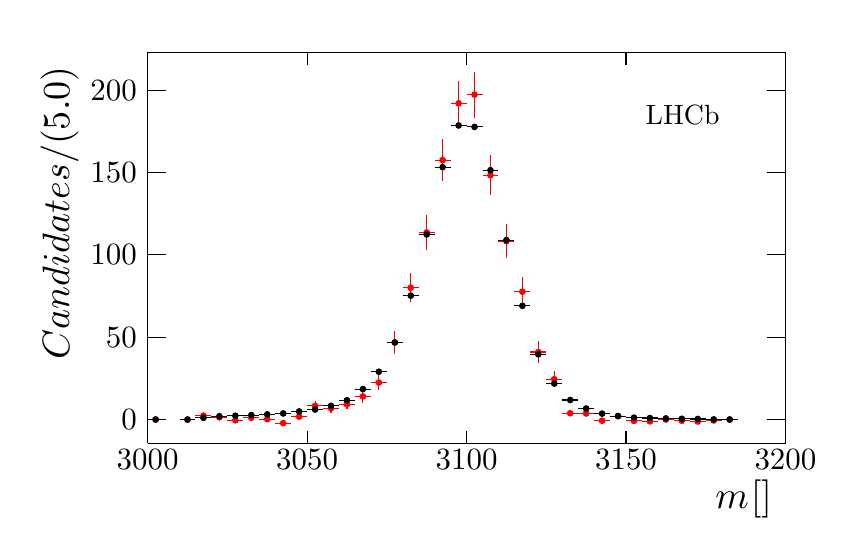
\begin{tikzpicture}
\pgfdeclareplotmark{cross} {
\pgfpathmoveto{\pgfpoint{-0.3\pgfplotmarksize}{\pgfplotmarksize}}
\pgfpathlineto{\pgfpoint{+0.3\pgfplotmarksize}{\pgfplotmarksize}}
\pgfpathlineto{\pgfpoint{+0.3\pgfplotmarksize}{0.3\pgfplotmarksize}}
\pgfpathlineto{\pgfpoint{+1\pgfplotmarksize}{0.3\pgfplotmarksize}}
\pgfpathlineto{\pgfpoint{+1\pgfplotmarksize}{-0.3\pgfplotmarksize}}
\pgfpathlineto{\pgfpoint{+0.3\pgfplotmarksize}{-0.3\pgfplotmarksize}}
\pgfpathlineto{\pgfpoint{+0.3\pgfplotmarksize}{-1.\pgfplotmarksize}}
\pgfpathlineto{\pgfpoint{-0.3\pgfplotmarksize}{-1.\pgfplotmarksize}}
\pgfpathlineto{\pgfpoint{-0.3\pgfplotmarksize}{-0.3\pgfplotmarksize}}
\pgfpathlineto{\pgfpoint{-1.\pgfplotmarksize}{-0.3\pgfplotmarksize}}
\pgfpathlineto{\pgfpoint{-1.\pgfplotmarksize}{0.3\pgfplotmarksize}}
\pgfpathlineto{\pgfpoint{-0.3\pgfplotmarksize}{0.3\pgfplotmarksize}}
\pgfpathclose
\pgfusepathqstroke
}
\pgfdeclareplotmark{cross*} {
\pgfpathmoveto{\pgfpoint{-0.3\pgfplotmarksize}{\pgfplotmarksize}}
\pgfpathlineto{\pgfpoint{+0.3\pgfplotmarksize}{\pgfplotmarksize}}
\pgfpathlineto{\pgfpoint{+0.3\pgfplotmarksize}{0.3\pgfplotmarksize}}
\pgfpathlineto{\pgfpoint{+1\pgfplotmarksize}{0.3\pgfplotmarksize}}
\pgfpathlineto{\pgfpoint{+1\pgfplotmarksize}{-0.3\pgfplotmarksize}}
\pgfpathlineto{\pgfpoint{+0.3\pgfplotmarksize}{-0.3\pgfplotmarksize}}
\pgfpathlineto{\pgfpoint{+0.3\pgfplotmarksize}{-1.\pgfplotmarksize}}
\pgfpathlineto{\pgfpoint{-0.3\pgfplotmarksize}{-1.\pgfplotmarksize}}
\pgfpathlineto{\pgfpoint{-0.3\pgfplotmarksize}{-0.3\pgfplotmarksize}}
\pgfpathlineto{\pgfpoint{-1.\pgfplotmarksize}{-0.3\pgfplotmarksize}}
\pgfpathlineto{\pgfpoint{-1.\pgfplotmarksize}{0.3\pgfplotmarksize}}
\pgfpathlineto{\pgfpoint{-0.3\pgfplotmarksize}{0.3\pgfplotmarksize}}
\pgfpathclose
\pgfusepathqfillstroke
}
\pgfdeclareplotmark{newstar} {
\pgfpathmoveto{\pgfqpoint{0pt}{\pgfplotmarksize}}
\pgfpathlineto{\pgfqpointpolar{44}{0.5\pgfplotmarksize}}
\pgfpathlineto{\pgfqpointpolar{18}{\pgfplotmarksize}}
\pgfpathlineto{\pgfqpointpolar{-20}{0.5\pgfplotmarksize}}
\pgfpathlineto{\pgfqpointpolar{-54}{\pgfplotmarksize}}
\pgfpathlineto{\pgfqpointpolar{-90}{0.5\pgfplotmarksize}}
\pgfpathlineto{\pgfqpointpolar{234}{\pgfplotmarksize}}
\pgfpathlineto{\pgfqpointpolar{198}{0.5\pgfplotmarksize}}
\pgfpathlineto{\pgfqpointpolar{162}{\pgfplotmarksize}}
\pgfpathlineto{\pgfqpointpolar{134}{0.5\pgfplotmarksize}}
\pgfpathclose
\pgfusepathqstroke
}
\pgfdeclareplotmark{newstar*} {
\pgfpathmoveto{\pgfqpoint{0pt}{\pgfplotmarksize}}
\pgfpathlineto{\pgfqpointpolar{44}{0.5\pgfplotmarksize}}
\pgfpathlineto{\pgfqpointpolar{18}{\pgfplotmarksize}}
\pgfpathlineto{\pgfqpointpolar{-20}{0.5\pgfplotmarksize}}
\pgfpathlineto{\pgfqpointpolar{-54}{\pgfplotmarksize}}
\pgfpathlineto{\pgfqpointpolar{-90}{0.5\pgfplotmarksize}}
\pgfpathlineto{\pgfqpointpolar{234}{\pgfplotmarksize}}
\pgfpathlineto{\pgfqpointpolar{198}{0.5\pgfplotmarksize}}
\pgfpathlineto{\pgfqpointpolar{162}{\pgfplotmarksize}}
\pgfpathlineto{\pgfqpointpolar{134}{0.5\pgfplotmarksize}}
\pgfpathclose
\pgfusepathqfillstroke
}
\definecolor{c}{rgb}{1,1,1};
\draw [color=c, fill=c] (0,0) rectangle (10,6.27517);
\draw [color=c, fill=c] (1.4,1.00403) rectangle (9.5,5.96141);
\definecolor{c}{rgb}{0,0,0};
\draw [c] (1.4,1.00403) -- (1.4,5.96141) -- (9.5,5.96141) -- (9.5,1.00403) -- (1.4,1.00403);
\definecolor{c}{rgb}{1,1,1};
\draw [color=c, fill=c] (1.4,1.00403) rectangle (9.5,5.96141);
\definecolor{c}{rgb}{0,0,0};
\draw [c] (1.4,1.00403) -- (1.4,5.96141) -- (9.5,5.96141) -- (9.5,1.00403) -- (1.4,1.00403);
\definecolor{c}{rgb}{1,0,0};
\draw [c,line width=0.4] (1.50125,1.30263) -- (1.50125,1.30542);
\draw [c,line width=0.4] (1.50125,1.30542) -- (1.50125,1.30821);
\draw [c,line width=0.4] (1.4,1.30542) -- (1.50125,1.30542);
\draw [c,line width=0.4] (1.50125,1.30542) -- (1.6025,1.30542);
\foreach \P in {(1.50125,1.30542)}{\draw[mark options={color=c,fill=c},mark size=2.402402pt,mark=*,mark size=1pt] plot coordinates {\P};}
\draw [c,line width=0.4] (1.90625,1.29609) -- (1.90625,1.3033);
\draw [c,line width=0.4] (1.90625,1.3033) -- (1.90625,1.31052);
\draw [c,line width=0.4] (1.805,1.3033) -- (1.90625,1.3033);
\draw [c,line width=0.4] (1.90625,1.3033) -- (2.0075,1.3033);
\foreach \P in {(1.90625,1.3033)}{\draw[mark options={color=c,fill=c},mark size=2.402402pt,mark=*,mark size=1pt] plot coordinates {\P};}
\draw [c,line width=0.4] (2.10875,1.32351) -- (2.10875,1.35585);
\draw [c,line width=0.4] (2.10875,1.35585) -- (2.10875,1.3882);
\draw [c,line width=0.4] (2.0075,1.35585) -- (2.10875,1.35585);
\draw [c,line width=0.4] (2.10875,1.35585) -- (2.21,1.35585);
\foreach \P in {(2.10875,1.35585)}{\draw[mark options={color=c,fill=c},mark size=2.402402pt,mark=*,mark size=1pt] plot coordinates {\P};}
\draw [c,line width=0.4] (2.31125,1.30958) -- (2.31125,1.33376);
\draw [c,line width=0.4] (2.31125,1.33376) -- (2.31125,1.35794);
\draw [c,line width=0.4] (2.21,1.33376) -- (2.31125,1.33376);
\draw [c,line width=0.4] (2.31125,1.33376) -- (2.4125,1.33376);
\foreach \P in {(2.31125,1.33376)}{\draw[mark options={color=c,fill=c},mark size=2.402402pt,mark=*,mark size=1pt] plot coordinates {\P};}
\draw [c,line width=0.4] (2.51375,1.28158) -- (2.51375,1.29593);
\draw [c,line width=0.4] (2.51375,1.29593) -- (2.51375,1.31029);
\draw [c,line width=0.4] (2.4125,1.29593) -- (2.51375,1.29593);
\draw [c,line width=0.4] (2.51375,1.29593) -- (2.615,1.29593);
\foreach \P in {(2.51375,1.29593)}{\draw[mark options={color=c,fill=c},mark size=2.402402pt,mark=*,mark size=1pt] plot coordinates {\P};}
\draw [c,line width=0.4] (2.71625,1.30607) -- (2.71625,1.32724);
\draw [c,line width=0.4] (2.71625,1.32724) -- (2.71625,1.34841);
\draw [c,line width=0.4] (2.615,1.32724) -- (2.71625,1.32724);
\draw [c,line width=0.4] (2.71625,1.32724) -- (2.8175,1.32724);
\foreach \P in {(2.71625,1.32724)}{\draw[mark options={color=c,fill=c},mark size=2.402402pt,mark=*,mark size=1pt] plot coordinates {\P};}
\draw [c,line width=0.4] (2.91875,1.30066) -- (2.91875,1.30973);
\draw [c,line width=0.4] (2.91875,1.30973) -- (2.91875,1.31879);
\draw [c,line width=0.4] (2.8175,1.30973) -- (2.91875,1.30973);
\draw [c,line width=0.4] (2.91875,1.30973) -- (3.02,1.30973);
\foreach \P in {(2.91875,1.30973)}{\draw[mark options={color=c,fill=c},mark size=2.402402pt,mark=*,mark size=1pt] plot coordinates {\P};}
\draw [c,line width=0.4] (3.12125,1.22885) -- (3.12125,1.25984);
\draw [c,line width=0.4] (3.12125,1.25984) -- (3.12125,1.29084);
\draw [c,line width=0.4] (3.02,1.25984) -- (3.12125,1.25984);
\draw [c,line width=0.4] (3.12125,1.25984) -- (3.2225,1.25984);
\foreach \P in {(3.12125,1.25984)}{\draw[mark options={color=c,fill=c},mark size=2.402402pt,mark=*,mark size=1pt] plot coordinates {\P};}
\draw [c,line width=0.4] (3.32375,1.31427) -- (3.32375,1.34164);
\draw [c,line width=0.4] (3.32375,1.34164) -- (3.32375,1.36902);
\draw [c,line width=0.4] (3.2225,1.34164) -- (3.32375,1.34164);
\draw [c,line width=0.4] (3.32375,1.34164) -- (3.425,1.34164);
\foreach \P in {(3.32375,1.34164)}{\draw[mark options={color=c,fill=c},mark size=2.402402pt,mark=*,mark size=1pt] plot coordinates {\P};}
\draw [c,line width=0.4] (3.52625,1.41873) -- (3.52625,1.47888);
\draw [c,line width=0.4] (3.52625,1.47888) -- (3.52625,1.53903);
\draw [c,line width=0.4] (3.425,1.47888) -- (3.52625,1.47888);
\draw [c,line width=0.4] (3.52625,1.47888) -- (3.6275,1.47888);
\foreach \P in {(3.52625,1.47888)}{\draw[mark options={color=c,fill=c},mark size=2.402402pt,mark=*,mark size=1pt] plot coordinates {\P};}
\draw [c,line width=0.4] (3.72875,1.39417) -- (3.72875,1.44886);
\draw [c,line width=0.4] (3.72875,1.44886) -- (3.72875,1.50354);
\draw [c,line width=0.4] (3.6275,1.44886) -- (3.72875,1.44886);
\draw [c,line width=0.4] (3.72875,1.44886) -- (3.83,1.44886);
\foreach \P in {(3.72875,1.44886)}{\draw[mark options={color=c,fill=c},mark size=2.402402pt,mark=*,mark size=1pt] plot coordinates {\P};}
\draw [c,line width=0.4] (3.93125,1.43498) -- (3.93125,1.49844);
\draw [c,line width=0.4] (3.93125,1.49844) -- (3.93125,1.5619);
\draw [c,line width=0.4] (3.83,1.49844) -- (3.93125,1.49844);
\draw [c,line width=0.4] (3.93125,1.49844) -- (4.0325,1.49844);
\foreach \P in {(3.93125,1.49844)}{\draw[mark options={color=c,fill=c},mark size=2.402402pt,mark=*,mark size=1pt] plot coordinates {\P};}
\draw [c,line width=0.4] (4.13375,1.52091) -- (4.13375,1.59922);
\draw [c,line width=0.4] (4.13375,1.59922) -- (4.13375,1.67754);
\draw [c,line width=0.4] (4.0325,1.59922) -- (4.13375,1.59922);
\draw [c,line width=0.4] (4.13375,1.59922) -- (4.235,1.59922);
\foreach \P in {(4.13375,1.59922)}{\draw[mark options={color=c,fill=c},mark size=2.402402pt,mark=*,mark size=1pt] plot coordinates {\P};}
\draw [c,line width=0.4] (4.33625,1.67561) -- (4.33625,1.77461);
\draw [c,line width=0.4] (4.33625,1.77461) -- (4.33625,1.8736);
\draw [c,line width=0.4] (4.235,1.77461) -- (4.33625,1.77461);
\draw [c,line width=0.4] (4.33625,1.77461) -- (4.4375,1.77461);
\foreach \P in {(4.33625,1.77461)}{\draw[mark options={color=c,fill=c},mark size=2.402402pt,mark=*,mark size=1pt] plot coordinates {\P};}
\draw [c,line width=0.4] (4.53875,2.14103) -- (4.53875,2.28403);
\draw [c,line width=0.4] (4.53875,2.28403) -- (4.53875,2.42702);
\draw [c,line width=0.4] (4.4375,2.28403) -- (4.53875,2.28403);
\draw [c,line width=0.4] (4.53875,2.28403) -- (4.64,2.28403);
\foreach \P in {(4.53875,2.28403)}{\draw[mark options={color=c,fill=c},mark size=2.402402pt,mark=*,mark size=1pt] plot coordinates {\P};}
\draw [c,line width=0.4] (4.74125,2.79202) -- (4.74125,2.97904);
\draw [c,line width=0.4] (4.74125,2.97904) -- (4.74125,3.16605);
\draw [c,line width=0.4] (4.64,2.97904) -- (4.74125,2.97904);
\draw [c,line width=0.4] (4.74125,2.97904) -- (4.8425,2.97904);
\foreach \P in {(4.74125,2.97904)}{\draw[mark options={color=c,fill=c},mark size=2.402402pt,mark=*,mark size=1pt] plot coordinates {\P};}
\draw [c,line width=0.4] (4.94375,3.45838) -- (4.94375,3.68121);
\draw [c,line width=0.4] (4.94375,3.68121) -- (4.94375,3.90404);
\draw [c,line width=0.4] (4.8425,3.68121) -- (4.94375,3.68121);
\draw [c,line width=0.4] (4.94375,3.68121) -- (5.045,3.68121);
\foreach \P in {(4.94375,3.68121)}{\draw[mark options={color=c,fill=c},mark size=2.402402pt,mark=*,mark size=1pt] plot coordinates {\P};}
\draw [c,line width=0.4] (5.14625,4.33817) -- (5.14625,4.6006);
\draw [c,line width=0.4] (5.14625,4.6006) -- (5.14625,4.86303);
\draw [c,line width=0.4] (5.045,4.6006) -- (5.14625,4.6006);
\draw [c,line width=0.4] (5.14625,4.6006) -- (5.2475,4.6006);
\foreach \P in {(5.14625,4.6006)}{\draw[mark options={color=c,fill=c},mark size=2.402402pt,mark=*,mark size=1pt] plot coordinates {\P};}
\draw [c,line width=0.4] (5.34875,5.03126) -- (5.34875,5.32096);
\draw [c,line width=0.4] (5.34875,5.32096) -- (5.34875,5.61066);
\draw [c,line width=0.4] (5.2475,5.32096) -- (5.34875,5.32096);
\draw [c,line width=0.4] (5.34875,5.32096) -- (5.45,5.32096);
\foreach \P in {(5.34875,5.32096)}{\draw[mark options={color=c,fill=c},mark size=2.402402pt,mark=*,mark size=1pt] plot coordinates {\P};}
\draw [c,line width=0.4] (5.55125,5.138) -- (5.55125,5.43167);
\draw [c,line width=0.4] (5.55125,5.43167) -- (5.55125,5.72534);
\draw [c,line width=0.4] (5.45,5.43167) -- (5.55125,5.43167);
\draw [c,line width=0.4] (5.55125,5.43167) -- (5.6525,5.43167);
\foreach \P in {(5.55125,5.43167)}{\draw[mark options={color=c,fill=c},mark size=2.402402pt,mark=*,mark size=1pt] plot coordinates {\P};}
\draw [c,line width=0.4] (5.75375,4.15356) -- (5.75375,4.40822);
\draw [c,line width=0.4] (5.75375,4.40822) -- (5.75375,4.66288);
\draw [c,line width=0.4] (5.6525,4.40822) -- (5.75375,4.40822);
\draw [c,line width=0.4] (5.75375,4.40822) -- (5.855,4.40822);
\foreach \P in {(5.75375,4.40822)}{\draw[mark options={color=c,fill=c},mark size=2.402402pt,mark=*,mark size=1pt] plot coordinates {\P};}
\draw [c,line width=0.4] (5.95625,3.35186) -- (5.95625,3.56938);
\draw [c,line width=0.4] (5.95625,3.56938) -- (5.95625,3.7869);
\draw [c,line width=0.4] (5.855,3.56938) -- (5.95625,3.56938);
\draw [c,line width=0.4] (5.95625,3.56938) -- (6.0575,3.56938);
\foreach \P in {(5.95625,3.56938)}{\draw[mark options={color=c,fill=c},mark size=2.402402pt,mark=*,mark size=1pt] plot coordinates {\P};}
\draw [c,line width=0.4] (6.15875,2.74492) -- (6.15875,2.92913);
\draw [c,line width=0.4] (6.15875,2.92913) -- (6.15875,3.11334);
\draw [c,line width=0.4] (6.0575,2.92913) -- (6.15875,2.92913);
\draw [c,line width=0.4] (6.15875,2.92913) -- (6.26,2.92913);
\foreach \P in {(6.15875,2.92913)}{\draw[mark options={color=c,fill=c},mark size=2.402402pt,mark=*,mark size=1pt] plot coordinates {\P};}
\draw [c,line width=0.4] (6.36125,2.02911) -- (6.36125,2.16296);
\draw [c,line width=0.4] (6.36125,2.16296) -- (6.36125,2.29682);
\draw [c,line width=0.4] (6.26,2.16296) -- (6.36125,2.16296);
\draw [c,line width=0.4] (6.36125,2.16296) -- (6.4625,2.16296);
\foreach \P in {(6.36125,2.16296)}{\draw[mark options={color=c,fill=c},mark size=2.402402pt,mark=*,mark size=1pt] plot coordinates {\P};}
\draw [c,line width=0.4] (6.56375,1.714) -- (6.56375,1.81741);
\draw [c,line width=0.4] (6.56375,1.81741) -- (6.56375,1.92082);
\draw [c,line width=0.4] (6.4625,1.81741) -- (6.56375,1.81741);
\draw [c,line width=0.4] (6.56375,1.81741) -- (6.665,1.81741);
\foreach \P in {(6.56375,1.81741)}{\draw[mark options={color=c,fill=c},mark size=2.402402pt,mark=*,mark size=1pt] plot coordinates {\P};}
\draw [c,line width=0.4] (6.76625,1.34466) -- (6.76625,1.38547);
\draw [c,line width=0.4] (6.76625,1.38547) -- (6.76625,1.42627);
\draw [c,line width=0.4] (6.665,1.38547) -- (6.76625,1.38547);
\draw [c,line width=0.4] (6.76625,1.38547) -- (6.8675,1.38547);
\foreach \P in {(6.76625,1.38547)}{\draw[mark options={color=c,fill=c},mark size=2.402402pt,mark=*,mark size=1pt] plot coordinates {\P};}
\draw [c,line width=0.4] (6.96875,1.34285) -- (6.96875,1.38303);
\draw [c,line width=0.4] (6.96875,1.38303) -- (6.96875,1.42321);
\draw [c,line width=0.4] (6.8675,1.38303) -- (6.96875,1.38303);
\draw [c,line width=0.4] (6.96875,1.38303) -- (7.07,1.38303);
\foreach \P in {(6.96875,1.38303)}{\draw[mark options={color=c,fill=c},mark size=2.402402pt,mark=*,mark size=1pt] plot coordinates {\P};}
\draw [c,line width=0.4] (7.17125,1.2726) -- (7.17125,1.29049);
\draw [c,line width=0.4] (7.17125,1.29049) -- (7.17125,1.30837);
\draw [c,line width=0.4] (7.07,1.29049) -- (7.17125,1.29049);
\draw [c,line width=0.4] (7.17125,1.29049) -- (7.2725,1.29049);
\foreach \P in {(7.17125,1.29049)}{\draw[mark options={color=c,fill=c},mark size=2.402402pt,mark=*,mark size=1pt] plot coordinates {\P};}
\draw [c,line width=0.4] (7.37375,1.31892) -- (7.37375,1.34896);
\draw [c,line width=0.4] (7.37375,1.34896) -- (7.37375,1.379);
\draw [c,line width=0.4] (7.2725,1.34896) -- (7.37375,1.34896);
\draw [c,line width=0.4] (7.37375,1.34896) -- (7.475,1.34896);
\foreach \P in {(7.37375,1.34896)}{\draw[mark options={color=c,fill=c},mark size=2.402402pt,mark=*,mark size=1pt] plot coordinates {\P};}
\draw [c,line width=0.4] (7.57625,1.26893) -- (7.57625,1.28814);
\draw [c,line width=0.4] (7.57625,1.28814) -- (7.57625,1.30735);
\draw [c,line width=0.4] (7.475,1.28814) -- (7.57625,1.28814);
\draw [c,line width=0.4] (7.57625,1.28814) -- (7.6775,1.28814);
\foreach \P in {(7.57625,1.28814)}{\draw[mark options={color=c,fill=c},mark size=2.402402pt,mark=*,mark size=1pt] plot coordinates {\P};}
\draw [c,line width=0.4] (7.77875,1.25931) -- (7.77875,1.28174);
\draw [c,line width=0.4] (7.77875,1.28174) -- (7.77875,1.30416);
\draw [c,line width=0.4] (7.6775,1.28174) -- (7.77875,1.28174);
\draw [c,line width=0.4] (7.77875,1.28174) -- (7.88,1.28174);
\foreach \P in {(7.77875,1.28174)}{\draw[mark options={color=c,fill=c},mark size=2.402402pt,mark=*,mark size=1pt] plot coordinates {\P};}
\draw [c,line width=0.4] (7.98125,1.30314) -- (7.98125,1.30552);
\draw [c,line width=0.4] (7.98125,1.30552) -- (7.98125,1.30791);
\draw [c,line width=0.4] (7.88,1.30552) -- (7.98125,1.30552);
\draw [c,line width=0.4] (7.98125,1.30552) -- (8.0825,1.30552);
\foreach \P in {(7.98125,1.30552)}{\draw[mark options={color=c,fill=c},mark size=2.402402pt,mark=*,mark size=1pt] plot coordinates {\P};}
\draw [c,line width=0.4] (8.18375,1.27222) -- (8.18375,1.29025);
\draw [c,line width=0.4] (8.18375,1.29025) -- (8.18375,1.30828);
\draw [c,line width=0.4] (8.0825,1.29025) -- (8.18375,1.29025);
\draw [c,line width=0.4] (8.18375,1.29025) -- (8.285,1.29025);
\foreach \P in {(8.18375,1.29025)}{\draw[mark options={color=c,fill=c},mark size=2.402402pt,mark=*,mark size=1pt] plot coordinates {\P};}
\draw [c,line width=0.4] (8.38625,1.2575) -- (8.38625,1.28049);
\draw [c,line width=0.4] (8.38625,1.28049) -- (8.38625,1.30349);
\draw [c,line width=0.4] (8.285,1.28049) -- (8.38625,1.28049);
\draw [c,line width=0.4] (8.38625,1.28049) -- (8.4875,1.28049);
\foreach \P in {(8.38625,1.28049)}{\draw[mark options={color=c,fill=c},mark size=2.402402pt,mark=*,mark size=1pt] plot coordinates {\P};}
\draw [c,line width=0.4] (8.58875,1.27825) -- (8.58875,1.29397);
\draw [c,line width=0.4] (8.58875,1.29397) -- (8.58875,1.30969);
\draw [c,line width=0.4] (8.4875,1.29397) -- (8.58875,1.29397);
\draw [c,line width=0.4] (8.58875,1.29397) -- (8.69,1.29397);
\foreach \P in {(8.58875,1.29397)}{\draw[mark options={color=c,fill=c},mark size=2.402402pt,mark=*,mark size=1pt] plot coordinates {\P};}
\draw [c,line width=0.4] (8.79125,1.30513) -- (8.79125,1.30582);
\draw [c,line width=0.4] (8.79125,1.30582) -- (8.79125,1.3065);
\draw [c,line width=0.4] (8.69,1.30582) -- (8.79125,1.30582);
\draw [c,line width=0.4] (8.79125,1.30582) -- (8.8925,1.30582);
\foreach \P in {(8.79125,1.30582)}{\draw[mark options={color=c,fill=c},mark size=2.402402pt,mark=*,mark size=1pt] plot coordinates {\P};}
\definecolor{c}{rgb}{0,0,0};
\draw [c,line width=0.4] (1.4,1.00403) -- (9.5,1.00403);
\draw [anchor= east] (9.5,0.301208) node[scale=1.37879, rotate=0]{$m_{\Jpsi} [\mevcc]$};
\draw [c,line width=0.4] (1.4,1.15651) -- (1.4,1.00403);
\draw [c,line width=0.4] (3.425,1.15651) -- (3.425,1.00403);
\draw [c,line width=0.4] (5.45,1.15651) -- (5.45,1.00403);
\draw [c,line width=0.4] (7.475,1.15651) -- (7.475,1.00403);
\draw [c,line width=0.4] (9.5,1.15651) -- (9.5,1.00403);
\draw [anchor=base] (1.4,0.665168) node[scale=1.11794, rotate=0]{3000};
\draw [anchor=base] (3.425,0.665168) node[scale=1.11794, rotate=0]{3050};
\draw [anchor=base] (5.45,0.665168) node[scale=1.11794, rotate=0]{3100};
\draw [anchor=base] (7.475,0.665168) node[scale=1.11794, rotate=0]{3150};
\draw [anchor=base] (9.5,0.665168) node[scale=1.11794, rotate=0]{3200};
\draw [c,line width=0.4] (1.4,5.96141) -- (9.5,5.96141);
\draw [c,line width=0.4] (1.4,5.80892) -- (1.4,5.96141);
\draw [c,line width=0.4] (3.425,5.80892) -- (3.425,5.96141);
\draw [c,line width=0.4] (5.45,5.80892) -- (5.45,5.96141);
\draw [c,line width=0.4] (7.475,5.80892) -- (7.475,5.96141);
\draw [c,line width=0.4] (9.5,5.80892) -- (9.5,5.96141);
\draw [c,line width=0.4] (1.4,1.00403) -- (1.4,5.96141);
\draw [anchor= east] (0.28,5.96141) node[scale=1.37879, rotate=90]{$\text{Candidates} / (5.0 \mevcc)$};
\draw [c,line width=0.4] (1.637,1.30579) -- (1.4,1.30579);
\draw [c,line width=0.4] (1.637,2.35093) -- (1.4,2.35093);
\draw [c,line width=0.4] (1.637,3.39607) -- (1.4,3.39607);
\draw [c,line width=0.4] (1.637,4.44121) -- (1.4,4.44121);
\draw [c,line width=0.4] (1.637,5.48635) -- (1.4,5.48635);
\draw [c,line width=0.4] (1.637,1.30579) -- (1.4,1.30579);
\draw [c,line width=0.4] (1.637,5.48635) -- (1.4,5.48635);
\draw [anchor= east] (1.4,1.30579) node[scale=1.11794, rotate=0]{0};
\draw [anchor= east] (1.4,2.35093) node[scale=1.11794, rotate=0]{50};
\draw [anchor= east] (1.4,3.39607) node[scale=1.11794, rotate=0]{100};
\draw [anchor= east] (1.4,4.44121) node[scale=1.11794, rotate=0]{150};
\draw [anchor= east] (1.4,5.48635) node[scale=1.11794, rotate=0]{200};
\draw [c,line width=0.4] (9.5,1.00403) -- (9.5,5.96141);
\draw [c,line width=0.4] (9.263,1.30579) -- (9.5,1.30579);
\draw [c,line width=0.4] (9.263,2.35093) -- (9.5,2.35093);
\draw [c,line width=0.4] (9.263,3.39607) -- (9.5,3.39607);
\draw [c,line width=0.4] (9.263,4.44121) -- (9.5,4.44121);
\draw [c,line width=0.4] (9.263,5.48635) -- (9.5,5.48635);
\draw [c,line width=0.4] (9.263,1.30579) -- (9.5,1.30579);
\draw [c,line width=0.4] (9.263,5.48635) -- (9.5,5.48635);
\draw [c,line width=0.4] (1.50125,1.30578) -- (1.50125,1.3059);
\draw [c,line width=0.4] (1.50125,1.3059) -- (1.50125,1.30602);
\draw [c,line width=0.4] (1.4,1.3059) -- (1.50125,1.3059);
\draw [c,line width=0.4] (1.50125,1.3059) -- (1.6025,1.3059);
\foreach \P in {(1.50125,1.3059)}{\draw[mark options={color=c,fill=c},mark size=2.402402pt,mark=*,mark size=1pt] plot coordinates {\P};}
\draw [c,line width=0.4] (1.90625,1.30594) -- (1.90625,1.30616);
\draw [c,line width=0.4] (1.90625,1.30616) -- (1.90625,1.30638);
\draw [c,line width=0.4] (1.805,1.30616) -- (1.90625,1.30616);
\draw [c,line width=0.4] (1.90625,1.30616) -- (2.0075,1.30616);
\foreach \P in {(1.90625,1.30616)}{\draw[mark options={color=c,fill=c},mark size=2.402402pt,mark=*,mark size=1pt] plot coordinates {\P};}
\draw [c,line width=0.4] (2.10875,1.32564) -- (2.10875,1.32732);
\draw [c,line width=0.4] (2.10875,1.32732) -- (2.10875,1.32899);
\draw [c,line width=0.4] (2.0075,1.32732) -- (2.10875,1.32732);
\draw [c,line width=0.4] (2.10875,1.32732) -- (2.21,1.32732);
\foreach \P in {(2.10875,1.32732)}{\draw[mark options={color=c,fill=c},mark size=2.402402pt,mark=*,mark size=1pt] plot coordinates {\P};}
\draw [c,line width=0.4] (2.31125,1.3454) -- (2.31125,1.34774);
\draw [c,line width=0.4] (2.31125,1.34774) -- (2.31125,1.35008);
\draw [c,line width=0.4] (2.21,1.34774) -- (2.31125,1.34774);
\draw [c,line width=0.4] (2.31125,1.34774) -- (2.4125,1.34774);
\foreach \P in {(2.31125,1.34774)}{\draw[mark options={color=c,fill=c},mark size=2.402402pt,mark=*,mark size=1pt] plot coordinates {\P};}
\draw [c,line width=0.4] (2.51375,1.35162) -- (2.51375,1.35412);
\draw [c,line width=0.4] (2.51375,1.35412) -- (2.51375,1.35663);
\draw [c,line width=0.4] (2.4125,1.35412) -- (2.51375,1.35412);
\draw [c,line width=0.4] (2.51375,1.35412) -- (2.615,1.35412);
\foreach \P in {(2.51375,1.35412)}{\draw[mark options={color=c,fill=c},mark size=2.402402pt,mark=*,mark size=1pt] plot coordinates {\P};}
\draw [c,line width=0.4] (2.71625,1.35893) -- (2.71625,1.36163);
\draw [c,line width=0.4] (2.71625,1.36163) -- (2.71625,1.36433);
\draw [c,line width=0.4] (2.615,1.36163) -- (2.71625,1.36163);
\draw [c,line width=0.4] (2.71625,1.36163) -- (2.8175,1.36163);
\foreach \P in {(2.71625,1.36163)}{\draw[mark options={color=c,fill=c},mark size=2.402402pt,mark=*,mark size=1pt] plot coordinates {\P};}
\draw [c,line width=0.4] (2.91875,1.36797) -- (2.91875,1.37088);
\draw [c,line width=0.4] (2.91875,1.37088) -- (2.91875,1.37379);
\draw [c,line width=0.4] (2.8175,1.37088) -- (2.91875,1.37088);
\draw [c,line width=0.4] (2.91875,1.37088) -- (3.02,1.37088);
\foreach \P in {(2.91875,1.37088)}{\draw[mark options={color=c,fill=c},mark size=2.402402pt,mark=*,mark size=1pt] plot coordinates {\P};}
\draw [c,line width=0.4] (3.12125,1.37986) -- (3.12125,1.38304);
\draw [c,line width=0.4] (3.12125,1.38304) -- (3.12125,1.38621);
\draw [c,line width=0.4] (3.02,1.38304) -- (3.12125,1.38304);
\draw [c,line width=0.4] (3.12125,1.38304) -- (3.2225,1.38304);
\foreach \P in {(3.12125,1.38304)}{\draw[mark options={color=c,fill=c},mark size=2.402402pt,mark=*,mark size=1pt] plot coordinates {\P};}
\draw [c,line width=0.4] (3.32375,1.40451) -- (3.32375,1.40816);
\draw [c,line width=0.4] (3.32375,1.40816) -- (3.32375,1.41181);
\draw [c,line width=0.4] (3.2225,1.40816) -- (3.32375,1.40816);
\draw [c,line width=0.4] (3.32375,1.40816) -- (3.425,1.40816);
\foreach \P in {(3.32375,1.40816)}{\draw[mark options={color=c,fill=c},mark size=2.402402pt,mark=*,mark size=1pt] plot coordinates {\P};}
\draw [c,line width=0.4] (3.52625,1.42825) -- (3.52625,1.43231);
\draw [c,line width=0.4] (3.52625,1.43231) -- (3.52625,1.43637);
\draw [c,line width=0.4] (3.425,1.43231) -- (3.52625,1.43231);
\draw [c,line width=0.4] (3.52625,1.43231) -- (3.6275,1.43231);
\foreach \P in {(3.52625,1.43231)}{\draw[mark options={color=c,fill=c},mark size=2.402402pt,mark=*,mark size=1pt] plot coordinates {\P};}
\draw [c,line width=0.4] (3.72875,1.47515) -- (3.72875,1.47991);
\draw [c,line width=0.4] (3.72875,1.47991) -- (3.72875,1.48468);
\draw [c,line width=0.4] (3.6275,1.47991) -- (3.72875,1.47991);
\draw [c,line width=0.4] (3.72875,1.47991) -- (3.83,1.47991);
\foreach \P in {(3.72875,1.47991)}{\draw[mark options={color=c,fill=c},mark size=2.402402pt,mark=*,mark size=1pt] plot coordinates {\P};}
\draw [c,line width=0.4] (3.93125,1.54443) -- (3.93125,1.55007);
\draw [c,line width=0.4] (3.93125,1.55007) -- (3.93125,1.55571);
\draw [c,line width=0.4] (3.83,1.55007) -- (3.93125,1.55007);
\draw [c,line width=0.4] (3.93125,1.55007) -- (4.0325,1.55007);
\foreach \P in {(3.93125,1.55007)}{\draw[mark options={color=c,fill=c},mark size=2.402402pt,mark=*,mark size=1pt] plot coordinates {\P};}
\draw [c,line width=0.4] (4.13375,1.68508) -- (4.13375,1.69218);
\draw [c,line width=0.4] (4.13375,1.69218) -- (4.13375,1.69927);
\draw [c,line width=0.4] (4.0325,1.69218) -- (4.13375,1.69218);
\draw [c,line width=0.4] (4.13375,1.69218) -- (4.235,1.69218);
\foreach \P in {(4.13375,1.69218)}{\draw[mark options={color=c,fill=c},mark size=2.402402pt,mark=*,mark size=1pt] plot coordinates {\P};}
\draw [c,line width=0.4] (4.33625,1.90395) -- (4.33625,1.91284);
\draw [c,line width=0.4] (4.33625,1.91284) -- (4.33625,1.92174);
\draw [c,line width=0.4] (4.235,1.91284) -- (4.33625,1.91284);
\draw [c,line width=0.4] (4.33625,1.91284) -- (4.4375,1.91284);
\foreach \P in {(4.33625,1.91284)}{\draw[mark options={color=c,fill=c},mark size=2.402402pt,mark=*,mark size=1pt] plot coordinates {\P};}
\draw [c,line width=0.4] (4.53875,2.27346) -- (4.53875,2.28476);
\draw [c,line width=0.4] (4.53875,2.28476) -- (4.53875,2.29605);
\draw [c,line width=0.4] (4.4375,2.28476) -- (4.53875,2.28476);
\draw [c,line width=0.4] (4.53875,2.28476) -- (4.64,2.28476);
\foreach \P in {(4.53875,2.28476)}{\draw[mark options={color=c,fill=c},mark size=2.402402pt,mark=*,mark size=1pt] plot coordinates {\P};}
\draw [c,line width=0.4] (4.74125,2.86463) -- (4.74125,2.87895);
\draw [c,line width=0.4] (4.74125,2.87895) -- (4.74125,2.89327);
\draw [c,line width=0.4] (4.64,2.87895) -- (4.74125,2.87895);
\draw [c,line width=0.4] (4.74125,2.87895) -- (4.8425,2.87895);
\foreach \P in {(4.74125,2.87895)}{\draw[mark options={color=c,fill=c},mark size=2.402402pt,mark=*,mark size=1pt] plot coordinates {\P};}
\draw [c,line width=0.4] (4.94375,3.63832) -- (4.94375,3.65582);
\draw [c,line width=0.4] (4.94375,3.65582) -- (4.94375,3.67331);
\draw [c,line width=0.4] (4.8425,3.65582) -- (4.94375,3.65582);
\draw [c,line width=0.4] (4.94375,3.65582) -- (5.045,3.65582);
\foreach \P in {(4.94375,3.65582)}{\draw[mark options={color=c,fill=c},mark size=2.402402pt,mark=*,mark size=1pt] plot coordinates {\P};}
\draw [c,line width=0.4] (5.14625,4.49096) -- (5.14625,4.5114);
\draw [c,line width=0.4] (5.14625,4.5114) -- (5.14625,4.53183);
\draw [c,line width=0.4] (5.045,4.5114) -- (5.14625,4.5114);
\draw [c,line width=0.4] (5.14625,4.5114) -- (5.2475,4.5114);
\foreach \P in {(5.14625,4.5114)}{\draw[mark options={color=c,fill=c},mark size=2.402402pt,mark=*,mark size=1pt] plot coordinates {\P};}
\draw [c,line width=0.4] (5.34875,5.01806) -- (5.34875,5.04012);
\draw [c,line width=0.4] (5.34875,5.04012) -- (5.34875,5.06218);
\draw [c,line width=0.4] (5.2475,5.04012) -- (5.34875,5.04012);
\draw [c,line width=0.4] (5.34875,5.04012) -- (5.45,5.04012);
\foreach \P in {(5.34875,5.04012)}{\draw[mark options={color=c,fill=c},mark size=2.402402pt,mark=*,mark size=1pt] plot coordinates {\P};}
\draw [c,line width=0.4] (5.55125,4.99957) -- (5.55125,5.02157);
\draw [c,line width=0.4] (5.55125,5.02157) -- (5.55125,5.04358);
\draw [c,line width=0.4] (5.45,5.02157) -- (5.55125,5.02157);
\draw [c,line width=0.4] (5.55125,5.02157) -- (5.6525,5.02157);
\foreach \P in {(5.55125,5.02157)}{\draw[mark options={color=c,fill=c},mark size=2.402402pt,mark=*,mark size=1pt] plot coordinates {\P};}
\draw [c,line width=0.4] (5.75375,4.45184) -- (5.75375,4.47216);
\draw [c,line width=0.4] (5.75375,4.47216) -- (5.75375,4.49247);
\draw [c,line width=0.4] (5.6525,4.47216) -- (5.75375,4.47216);
\draw [c,line width=0.4] (5.75375,4.47216) -- (5.855,4.47216);
\foreach \P in {(5.75375,4.47216)}{\draw[mark options={color=c,fill=c},mark size=2.402402pt,mark=*,mark size=1pt] plot coordinates {\P};}
\draw [c,line width=0.4] (5.95625,3.56746) -- (5.95625,3.5847);
\draw [c,line width=0.4] (5.95625,3.5847) -- (5.95625,3.60193);
\draw [c,line width=0.4] (5.855,3.5847) -- (5.95625,3.5847);
\draw [c,line width=0.4] (5.95625,3.5847) -- (6.0575,3.5847);
\foreach \P in {(5.95625,3.5847)}{\draw[mark options={color=c,fill=c},mark size=2.402402pt,mark=*,mark size=1pt] plot coordinates {\P};}
\draw [c,line width=0.4] (6.15875,2.73591) -- (6.15875,2.74963);
\draw [c,line width=0.4] (6.15875,2.74963) -- (6.15875,2.76335);
\draw [c,line width=0.4] (6.0575,2.74963) -- (6.15875,2.74963);
\draw [c,line width=0.4] (6.15875,2.74963) -- (6.26,2.74963);
\foreach \P in {(6.15875,2.74963)}{\draw[mark options={color=c,fill=c},mark size=2.402402pt,mark=*,mark size=1pt] plot coordinates {\P};}
\draw [c,line width=0.4] (6.36125,2.12331) -- (6.36125,2.1337);
\draw [c,line width=0.4] (6.36125,2.1337) -- (6.36125,2.14408);
\draw [c,line width=0.4] (6.26,2.1337) -- (6.36125,2.1337);
\draw [c,line width=0.4] (6.36125,2.1337) -- (6.4625,2.1337);
\foreach \P in {(6.36125,2.1337)}{\draw[mark options={color=c,fill=c},mark size=2.402402pt,mark=*,mark size=1pt] plot coordinates {\P};}
\draw [c,line width=0.4] (6.56375,1.75436) -- (6.56375,1.76207);
\draw [c,line width=0.4] (6.56375,1.76207) -- (6.56375,1.76978);
\draw [c,line width=0.4] (6.4625,1.76207) -- (6.56375,1.76207);
\draw [c,line width=0.4] (6.56375,1.76207) -- (6.665,1.76207);
\foreach \P in {(6.56375,1.76207)}{\draw[mark options={color=c,fill=c},mark size=2.402402pt,mark=*,mark size=1pt] plot coordinates {\P};}
\draw [c,line width=0.4] (6.76625,1.54787) -- (6.76625,1.55355);
\draw [c,line width=0.4] (6.76625,1.55355) -- (6.76625,1.55923);
\draw [c,line width=0.4] (6.665,1.55355) -- (6.76625,1.55355);
\draw [c,line width=0.4] (6.76625,1.55355) -- (6.8675,1.55355);
\foreach \P in {(6.76625,1.55355)}{\draw[mark options={color=c,fill=c},mark size=2.402402pt,mark=*,mark size=1pt] plot coordinates {\P};}
\draw [c,line width=0.4] (6.96875,1.44145) -- (6.96875,1.44572);
\draw [c,line width=0.4] (6.96875,1.44572) -- (6.96875,1.44999);
\draw [c,line width=0.4] (6.8675,1.44572) -- (6.96875,1.44572);
\draw [c,line width=0.4] (6.96875,1.44572) -- (7.07,1.44572);
\foreach \P in {(6.96875,1.44572)}{\draw[mark options={color=c,fill=c},mark size=2.402402pt,mark=*,mark size=1pt] plot coordinates {\P};}
\draw [c,line width=0.4] (7.17125,1.37775) -- (7.17125,1.38088);
\draw [c,line width=0.4] (7.17125,1.38088) -- (7.17125,1.384);
\draw [c,line width=0.4] (7.07,1.38088) -- (7.17125,1.38088);
\draw [c,line width=0.4] (7.17125,1.38088) -- (7.2725,1.38088);
\foreach \P in {(7.17125,1.38088)}{\draw[mark options={color=c,fill=c},mark size=2.402402pt,mark=*,mark size=1pt] plot coordinates {\P};}
\draw [c,line width=0.4] (7.37375,1.34711) -- (7.37375,1.3495);
\draw [c,line width=0.4] (7.37375,1.3495) -- (7.37375,1.35188);
\draw [c,line width=0.4] (7.2725,1.3495) -- (7.37375,1.3495);
\draw [c,line width=0.4] (7.37375,1.3495) -- (7.475,1.3495);
\foreach \P in {(7.37375,1.3495)}{\draw[mark options={color=c,fill=c},mark size=2.402402pt,mark=*,mark size=1pt] plot coordinates {\P};}
\draw [c,line width=0.4] (7.57625,1.32764) -- (7.57625,1.3294);
\draw [c,line width=0.4] (7.57625,1.3294) -- (7.57625,1.33115);
\draw [c,line width=0.4] (7.475,1.3294) -- (7.57625,1.3294);
\draw [c,line width=0.4] (7.57625,1.3294) -- (7.6775,1.3294);
\foreach \P in {(7.57625,1.3294)}{\draw[mark options={color=c,fill=c},mark size=2.402402pt,mark=*,mark size=1pt] plot coordinates {\P};}
\draw [c,line width=0.4] (7.77875,1.32289) -- (7.77875,1.32445);
\draw [c,line width=0.4] (7.77875,1.32445) -- (7.77875,1.32601);
\draw [c,line width=0.4] (7.6775,1.32445) -- (7.77875,1.32445);
\draw [c,line width=0.4] (7.77875,1.32445) -- (7.88,1.32445);
\foreach \P in {(7.77875,1.32445)}{\draw[mark options={color=c,fill=c},mark size=2.402402pt,mark=*,mark size=1pt] plot coordinates {\P};}
\draw [c,line width=0.4] (7.98125,1.31813) -- (7.98125,1.31947);
\draw [c,line width=0.4] (7.98125,1.31947) -- (7.98125,1.3208);
\draw [c,line width=0.4] (7.88,1.31947) -- (7.98125,1.31947);
\draw [c,line width=0.4] (7.98125,1.31947) -- (8.0825,1.31947);
\foreach \P in {(7.98125,1.31947)}{\draw[mark options={color=c,fill=c},mark size=2.402402pt,mark=*,mark size=1pt] plot coordinates {\P};}
\draw [c,line width=0.4] (8.18375,1.31364) -- (8.18375,1.31472);
\draw [c,line width=0.4] (8.18375,1.31472) -- (8.18375,1.3158);
\draw [c,line width=0.4] (8.0825,1.31472) -- (8.18375,1.31472);
\draw [c,line width=0.4] (8.18375,1.31472) -- (8.285,1.31472);
\foreach \P in {(8.18375,1.31472)}{\draw[mark options={color=c,fill=c},mark size=2.402402pt,mark=*,mark size=1pt] plot coordinates {\P};}
\draw [c,line width=0.4] (8.38625,1.31199) -- (8.38625,1.31296);
\draw [c,line width=0.4] (8.38625,1.31296) -- (8.38625,1.31393);
\draw [c,line width=0.4] (8.285,1.31296) -- (8.38625,1.31296);
\draw [c,line width=0.4] (8.38625,1.31296) -- (8.4875,1.31296);
\foreach \P in {(8.38625,1.31296)}{\draw[mark options={color=c,fill=c},mark size=2.402402pt,mark=*,mark size=1pt] plot coordinates {\P};}
\draw [c,line width=0.4] (8.58875,1.30708) -- (8.58875,1.30756);
\draw [c,line width=0.4] (8.58875,1.30756) -- (8.58875,1.30803);
\draw [c,line width=0.4] (8.4875,1.30756) -- (8.58875,1.30756);
\draw [c,line width=0.4] (8.58875,1.30756) -- (8.69,1.30756);
\foreach \P in {(8.58875,1.30756)}{\draw[mark options={color=c,fill=c},mark size=2.402402pt,mark=*,mark size=1pt] plot coordinates {\P};}
\draw [c,line width=0.4] (8.79125,1.30579) -- (8.79125,1.30592);
\draw [c,line width=0.4] (8.79125,1.30592) -- (8.79125,1.30605);
\draw [c,line width=0.4] (8.69,1.30592) -- (8.79125,1.30592);
\draw [c,line width=0.4] (8.79125,1.30592) -- (8.8925,1.30592);
\foreach \P in {(8.79125,1.30592)}{\draw[mark options={color=c,fill=c},mark size=2.402402pt,mark=*,mark size=1pt] plot coordinates {\P};}
\draw [anchor= west] (7.6,5.17701) node[scale=1.00614, rotate=0]{LHCb};
\end{tikzpicture}
}
    \caption{}
    \label{jpsiPlot}
  \end{subfigure}
\caption{Comparison of the intermediate state particles mass distributions between \Bs and \Bd.
         The plots are background subtracted. Top row shows the \mkpi distribution before (left)
         and after (right) correcting for angular acceptance effects. The \jpsi mass background subtracted
         distribution is shown at the bottom. It was checked that the acceptance correction has negligible
         effects on the shapes of the \jpsi mass distributions.}
\end{figure}

While the \Bs and \Bd background subtracted muon pair mass background subtracted, $\mmumu$, have very similar shapes, the \mkpi spectra exhibit different shapes.
Indeed, the \Bs \mkpi \sPlot of \figref{mkpiPlot_raw} seems to be slightly distorted compared to the one of \Bd \mkpi.
Since there is no \aprior reason why the \Kstarz \pwave
should have different shape between \BsJpsiKst and \BdJpsiKst; This could indicate the presence of interference between
the $\kaon\pi$ \swave and the \Kstarz, which may be stronger in the \Bs decays compared to the \Bd ones. In order
to check the validity of this hypothesis, two additional studies are performed. First it was checked that the non-resonant
background treatment propagated to the \sWeights was not responsible for this behavior. Indeed, no significant difference
between the \Bs \mkpi spectrum using \sWeights computed with and without simulated data injection was found. Second, the \mkpi
is corrected for angular acceptance effects, by weighting each candidate with the inverse of the acceptance function of \equref{eff_func_new}.
This way the interference between the $\kaon\pi$ \swave and the \Kstarz \pwave vanishes, since
for a perfect acceptance the interference terms in \tabref{ang_terms}, integrated over all angles, evaluate to zero.
This is demonstrated in \figref{mkpiPlot_eff}. The \Bs \mkpi distribution is closer to the one of the \Bd after applying
the efficiency correction. This is a clear indication of the presence of stronger interference in the \Bs case compared to the \Bd.

%%%%%%%%%%%%%%%%%%%%%%%%%%%%%%%%%%%%%%%%%%%%%%%%
\subsection{Production and Detection Asymmetries}
\label{experimentalAssym}
%%%%%%%%%%%%%%%%%%%%%%%%%%%%%%%%%%%%%%%%%%%%%%%%
The nature of the current analysis is such that it is affected by asymmetries related to experimental effects.
Particularly, the difference between the number of observed \BsJpsiKst and \BsbarJpsiKst decays is related to the
main parameters of interest, introduced in \secref{cp_assymetries_and_total_decay_rate}. These parameters essentially
quantify the direct \CP asymmetry between the previous decays.
Considering now the case where collisions at the \lhc would favor the \BsJpsiKst decay over its \CP conjugate, \BsbarJpsiKst;
or that the detector might have different efficiency for positive and negative kaons (or pions),
then the observed $\Acp{}$ will be biased by these experimental effects. In fact it happens so that both of these effects
are present. The first one, where the creation of a \Bs or \Bsb is favoured is labelled as  production asymmetry, $\Aprod$,
whereas the second effect is labelled as detection asymmetry, $\Adet$. The production and detection
asymmetries are defined in the following equation:

\begin{equation}
\centering
         \Aprod = \frac{ \crosSec{\Bsb} - \crosSec{\Bs} }{\crosSec{\Bsb} + \crosSec{\Bs}}
  \quad  \Adet  = \frac{ \effDet{\Kstarz} - \effDet{\Kstarzb} }{\effDet{\Kstarz} + \effDet{\Kstarzb}},
\label{exp_asym_def}
\end{equation}

\noindent where $\sigma$ is the production cross section of either \Bs or \Bb , whereas \edet is the efficiency
of detecting \Bs(\Bsb) decays into the final state which is a $\jpsi\Kstarzb$($\jpsi\Kstarz$), see also \secref{cp_assymetries_and_total_decay_rate}.
Both of the production and detection asymmetries have to be estimated so that the experimentally measured asymmetry, $\Acp{\rm raw}$,
defined in \equref{acp_mes}, can be corrected for as follows:

\begin{equation}
\centering
\Acp\;(\BsJpsiKst) = \Acp{\rm raw} +\Adet - \kappa\Aprod,
\label{acp_corrected}
\end{equation}

\noindent where the corrected asymmetry \Acp\;(\BsJpsiKst) is related to the \BsJpsiKst decay
amplitudes, defined in \equref{ang_terms}, as:

\begin{align}
\centering
  \Acp\;(\BsJpsiKst&) = \nonumber \\
  = &\frac{\totAmp{\BsbarJpsiKst} - \totAmp{\BsJpsiKst}}{\totAmp{\BsbarJpsiKst} + \totAmp{\BsJpsiKst}}.
\label{acp_corrected_amps}
\end{align}

\noindent The factor $\kappa$ of \equref{acp_corrected} accounts for the dilution due to $\Bs-\Bsb$
oscillations \cite{LHCb-PAPER-2013-018} and is:

\begin{equation}
  \centering
 \kappa = \frac{\int_0^\infty  e^{-\Gamma_s t} \cos \!\left( \Delta m_s t \right ) \varepsilon(t)\mathrm{d}t}{\int_0^\infty  e^{-\Gamma_s t} \cosh \left( \frac{\Delta \Gamma_s}{2} t \right ) \varepsilon(t)\mathrm{d}t}.
\label{kappa}
\end{equation}

\noindent It evaluates to $0.06\%$, which implies that the $\Bs-\Bsb$ oscillation frequency is large compared to the
average lifetime, $\Gamma_s$. As a result the production asymmetry is nearly completely washed out.
The quantities $\Delta\Gamma_s$ and $\Delta m_s$ have been introduced in \secref{Phenomenology},
while the decay time efficiency function $\varepsilon(t)$ is estimated on background subtracted \BsJpsiKst
data and parameterized as in \cite{LHCb-PAPER-2014-053}.

% with a the function $\varepsilon(t)= \frac{[1+\beta(t-t_0)][a(t-t0)]^n}{1+[a(t-t_0)]^n}$ found

Using the result from the dedicated \lhcb measurement of the production asymmetry \cite{LHCb-PAPER-2014-042}
and replacing the yield fractions in intervals of \Bs momentum of Table 3 in the same reference with the background
subtracted \BsJpsiKst ones of the current analysis, one gets the following production asymmetry:

\begin{equation}
    \centering
    \Aprod = (-1.64 \pm 2.28 \stat \pm 0.55 \syst).
  \label{prod_assym}
\end{equation}

\noindent The detection asymmetry is computed starting from the \lhcb study of the detection asymmetry
in \cite{LHCb-PAPER-2014-013} and weighting the kaon momentum distribution to much the observed
distribution in \BsJpsiKst data. The result is:

\begin{equation}
    \centering
    \Adet  = (-1.086 \pm 0.531 \stat).
  \label{det_assym}
\end{equation}

%%%%%%%%%%%%%%%%%%%%%%%%%%%%%%%%%%%%%%%%%%%%%%%%
\subsection{Likelihood fit and Total Decay Rate}
\label{Total_Decay_Rate}
%%%%%%%%%%%%%%%%%%%%%%%%%%%%%%%%%%%%%%%%%%%%%%%%

Nearly all the necessary ingredients to fit for the parameters of interest are covered in the previous subsections.
However there are a few important details remaining. The current subsection addresses the
implications arising from the necessary splitting of the data in slices and the impact of this in the adopted
fitting strategy. Lastly but most importantly the issue of defining
the polarization dependant \CP asymmetries, \Acp{k}, as free parameters in the angular fit and how this becomes
relevant in the normalization of the \pdfs involved is discussed in the last part of the current subsection.

\subsubsection{Simultaneous likelihood fit}
\label{Simutaneous_Likelihood_fit}
There are several reasons as to why the data are divided into sub-samples.
For example, the special treatment of the \mkpi dependence, as described in \secref{Kpi_Invariant_mass}
requires that the data is split in four \mkpi intervals. This implies that for each data category, a
corresponding component \pdf must be defined. Some parameters of interest differ between the categories
while some others are shared. In order to avoid performing four independent fits and subsequently averaging the common parameters
of interest, a simultaneous fit is implemented. In a simultaneous fit each component \pdf is assigned to a certain part of the data
such that the corresponding component \pdf is invoked when the total \pdf is evaluated. The current section summarizes
all the categories that the data is split into and the implications arising from this. Lastly a brief insight in some aspects
of the likelihood parameter estimation method are included.

The first data category is related to the fact that the angular \pdf terms of \tabref{ang_distr} cannot describe both \BsJpsiKst
and \BsbarJpsiKst. There is a relative minus sign difference in the imaginary terms originating from complex conjugating the decay
amplitude of \BsJpsiKst. For reasons explain in \secref{penguin_formalism} the \BsJpsiKst decays always have a negative kaon in
the final state and \viceversa in the case of \BsbarJpsiKst decays. Thus the data must be split according to the charge of
the kaon. Furthermore, as can be seen in \tabref{moms_comp_signs} the agreement between the \BsJpsiKst and \BsbarJpsiKst samples
is sufficient for them to be averaged into one set of efficiency moments. However, the angular acceptance as described in \secref{Accceptance}
is calculated separately for these two samples. This is done to avoid involving the $\Acp{i}$ parameters of interest
in the estimation of the efficiency moments, which significantly simplifies the necessary computation.
Note that the $\Acp{i}$ parameters are used to average the \BsJpsiKst and \BsbarJpsiKst decay amplitudes into one parameter,
more details in \secref{cp_assymetries_and_total_decay_rate}.

\begin{table}[t]
\centering
\begin{tabular}{c c c c c}
  \hline
              & interval 1 & interval 2 & interval 3 & interval 4\\
  \hline
  \mkpi range & $ [826,861) $ & $ [861,896) $ & $ [896,931) $ & $ [931,966] $ \\
  \CSP factor & $ 0.9681 $    & $ 0.9312 $    & $ 0.9519 $    & $ 0.9880 $ \\  \hline
\end{tabular}
\caption{Definitions of \mkpi intervals and the corresponding \CSP factor values.}
\label{csp_vals}
\end{table}

The next observable used to split the data is already mentioned in \secref{Kpi_Invariant_mass} that dealt with the \mkpi dependence.
There are four \mkpi intervals defining four more categories in the data. Furthermore, and contrary to the above-mentioned data category, there
are parameters of interest that are different in each \mkpi interval. Namely the \swave fraction $\fS{}$ and phase $\deltaS{}$.
In addition, the \CSP factors of \secref{Kpi_Invariant_mass} need to be calculated and inserted separately for each component \pdf resulting in
\tabref{csp_vals}, where the \CSP factors are shown for each \mkpi interval. The acceptance is also split in the \mkpi category
since it was found to vary significantly between \mkpi intervals, see \tabref{moms_final_neg} and \tabref{moms_final_pos}.
The \mkpi intervals chosen are shown in \tabref{csp_vals}.

The data categories described above result in a simultaneous fit consisting of eight categories.
A single angular acceptance is computed form the combined 2011 and 2012 data samples on grounds of
tables \tabref{moms_comp_periods_pos} and \tabref{moms_comp_periods_neg}.

Having addressed the simultaneous nature of the fit it is interesting to provide an insight on
the connection between a \pdf and the likelihood estimation of the parameters of interest.
Thus, starting from any \pdf $\mathcal{P}$ a likelihood function can be built as:

\begin{equation}
  \centering
L(\vec{p};\vec{x}) = \prod_e^n \mathcal{P}(\vec{x};\vec{p}).
\label{likelihood}
\end{equation}

\noindent By definition the likelihood function is the product of probabilities of every candidate according to the
 given \pdf. Note that, contrary to the \pdf, the likelihood is a function of the parameters given all the candidates in the data.
It is useful to realize that at the maximum of the likelihood function one gets the best estimate for the parameters of
interest, $\vec{p}$, given the data, $\vec{x}$. The inverse of the covariance matrix for the estimated parameters is given
by the negative second derivative of the log likelihood at the maximum,

\begin{equation}
  \centering
\left( V^{-1} \right)_{ij} = - \left. \frac{\partial^2\ln L}{\partial p_1 \partial p_2} \right|_{ \vec{p}_{\rm\bf max}}.
\label{covariance}
\end{equation}

Regarding the concept of the extended likelihood: In \equref{likelihood} the number of candidates is fixed.
However, it is possible to extend the previous equation such that the expected number of candidates shows up as a parameter in the likelihood
function and can thus be estimated. This is useful in cases where the \pdf consists of a sum over two species, such as signal and background,
or if the expected number of candidates depends on the parameters of interest $\vec{p}$. For the current analysis, the latter is
exploited in order to estimate the $\Acp{i}$ asymmetries in the fit. The \pdf is extended by multiplying it with the Poisson
probability to observe $n$ events when expecting $\expEvnts$ candidates, see \equref{extlikelihood}.
The expected number of candidates $\expEvnts$ depends on the
parameters of interest which increases the statistical uncertainties. This is because the likelihood has more freedom
as the number of parameters increases and thus the shape of the likelihood becomes less steep leading to larger statistical
uncertainty.

\begin{equation}
  \centering
L(\vec{p};\vec{x}) = P(n;\expEvnts) \; \prod_e^n \mathcal{P}(\vec{x};\vec{p}),
\label{extlikelihood}
\end{equation}

For purely practical reasons one would typically choose to minimize the negative logarithm of the likelihood, which after some simple
algebra and using the well known expression of the Poisson distribution results in:

\begin{align}
  \centering
  -\nll &= -\ln\left( \frac{\expEvnts}{n\,!} e^{-\expEvnts } \right) - \ln\left( \prod_e^n \mathcal{P}(\vec{x};\vec{p}) \right)  \nonumber \\
        &= - n\ln(\expEvnts) + \expEvnts  + \ln n! - \sum_e^n \ln\parenthesis{\mathcal{P}(\vec{x};\vec{p})} \nonumber \\
        &=  \expEvnts  - \sum_e^n \ln\parenthesis{\expEvnts \; \mathcal{P}(\vec{x};\vec{p}) } + {\rm const}.
\label{extloglikelihood}
\end{align}

\noindent Note that constant terms in the likelihood, like $\ln n!$, affect neither the shape of the likelihood
nor the position of the minimum and can thus be omitted.

\subsubsection{\CP asymmetries as free parameters}
\label{cp_assymetries_and_total_decay_rate}
The raw asymmetry, $\Acp{\rm raw}$, discussed in \secref{experimentalAssym}, can be measured by counting
$\BsbarJpsiKst$ and $\BsJpsiKst$ decays and use them to determine:

\begin{equation}
\Acp{\text{raw}} \equiv \frac{\Nplus - \Nminus}{\Nplus + \Nminus},
\label{acp_mes}
\end{equation}

\noindent where $\Nplus$ and $\Nminus$ are the number of observed \BsbarJpsiKst and \BsJpsiKst respectively.
Going one step further, $\Acp{\text{raw}}$ can be implemented as a parameter to be estimated in the fit. The advantage
is that the statistical uncertainty propagation for these parameters is implicit in the likelihood thus avoiding
explicit calculations. In addition, the above quantities can then be estimated separately for each polarization.
In order to vary $\Acp{\text{raw}}$ in the fit it is necessary to re-parameterize them as follows:

\begin{align}
  \label{acp_param}
\Acp{i} = \frac{\Nplus\AmpPlSq{i} - \Nminus\AmpMnSq{i}}{\Nplus\AmpPlSq{i} + \Nminus\AmpMnSq{i} } & \\
\text{and} \quad \AmpSq{i} = &\frac{ \Nplus \AmpPlSq{i} - \Nminus\AmpMnSq{i}}{\Nplus + \Nminus},
\end{align}

\noindent where $\AmpPlSq{i}$ and $\AmpMnSq{i}$ are the polarized amplitude in the \BsbarJpsiKst
and \BsJpsiKst samples respectively. The above equations can be solved for $\AmpPlSq{i}$ and $\AmpMnSq{i}$. The idea
is that the latter parameters will be used as amplitudes for the \BsbarJpsiKst and \BsJpsiKst \pdfs respectively.
This way both samples are fitted simultaneously in one fit. Solving \equref{acp_param} for $\AmpSq{\pm}$ yields:

\begin{equation}
\AmpPlSq{i} = \xi \; \AmpSq{i} (1+\Acp{i}) \,\, \text{and}\;\; \AmpMnSq{i} = \frac{\xi}{2\xi-1} \AmpSq{i} (1-\Acp{i}).
\label{acp_free}
\end{equation}

\noindent The $\AmpPlSq{i}$ and $\AmpMnSq{i}$ are the amplitude expressions that are used along with the angular functions of \tabref{ang_terms}.
The normalization factors in front of them can be re-expressed as function of $\Acp{\text{raw}}$ using \equref{acp_mes}.

\begin{align}
\xi = \frac{\Nplus+\Nminus}{2\Nplus} &= \frac{1}{2}\left( 1 + \frac{\yieldMn{}}{\yieldPl{}}\right) = \nonumber \\
                                     &= \frac{1}{2}\left( 1 + \frac{1-\Acp{\text{raw}}}{1+\Acp{\text{raw}}}\right) =
                                        \frac{1}{1+\Acp{\text{raw}}},  \\
\frac{\xi}{2\xi-1} = \frac{1}{2-\nicefrac{1}{\xi}} &= \frac{1}{1-\sum_i\Acp{\text{raw}}}.
\label{amp_norms}
\end{align}

\noindent Now, the quantities that are actually estimated in the likelihood fit are the $\AmpSq{i}$ with $i:\{0,\parallel,\perp,S\}$.
Having said that, and by looking at \equref{acp_free}, one understands that in order for $\AmpPlSq{i}$ and $\AmpMnSq{i}$
to be meaningful and consistent, the sum of all amplitudes $\sum\AmpSq{i}$ (with $i:{0,\parallel,\perp,S}$ ) must add up to one.
Thus imposing the condition $\sum\AmpSq{i} = 1$ one can re-express the $\AmpSq{i}$ as relative fractions:

\begin{equation}
\AmpSq{S} = \fS{} \;\;\;\text{and}\;\;\; \AmpSq{k} = (1-\fS{})\fP{k}.
\label{amps_param}
\end{equation}

\noindent Note that the \pwave fractions are also constrained so that they add up to one by imposing $\sum\fP{k}=1$ with $k:\{0,\parallel,\perp\}$.
The fractions $\fP{k}$ and $\fS{}$ are the actual parameters that one wishes to estimate and correspond to these used in the subsequent analysis of
\chapref{Penguins}. The final expressions of the $\AmpSqPm{i}$ after the above is given by:

\begin{equation}
\AmpSqPm{k} = \frac{1\pm\Acp{k}}{1\pm\sum_i\Acp{i}}  (1-\fS{})\fP{k}  \;\;\; \text{and}\;\;\; \AmpSqPm{S} = \frac{1\pm\Acp{S}}{1\pm\sum_i\Acp{i}} \; \fS{},
\label{amps_final}
\end{equation}

\noindent where the $i$ index runs through all amplitudes whereas $k$ only runs through the \pwave amplitudes.

There is one final step required to build the complete extended \pdf. That is the normalization of each component \pdf. Tempting as it might be to
normalize the component \pdfs to the number of observed candidates it would be wrong since the observed number of candidates are diluted by production and detection
asymmetry. Given that the parameters of interest, $\Acp{i}$, quantify the difference between the observed \BsbarJpsiKst and \BsJpsiKst decays, it follows that
the observed number of these decays need to be corrected for. With input from \secref{experimentalAssym} where the production and detection
asymmetries were estimated, the observed yields are made dependent on the $\Acp{i}$ asymmetry as:

\begin{subequations}
  \label{acp_yields}
  \begin{align}
    \yieldPl{\CP} &= \frac{ \yieldRaw{\text{total}} }{2} \left( \fS{}\; \Acp{S} + \sum_k^{0,\parallel,\perp} (1-\fS{})\fP{k}\Acp{k}  \right), \\
    \yieldMn{\CP} &=  \yieldRaw{\text{total}} - \yieldPl{\CP}
  \end{align}
\end{subequations}

\noindent and then subsequently corrected for the production and detection asymmetry resulting in:

\begin{equation}
\yield{\pm} = \yield{\pm}_{\CP}  \left( 1 \pm \Adet \mp \Aprod \right).
\label{norm_yields}
\end{equation}

\noindent The above yields are the expected number of candidates in the extended likelihood term of the \pdfs as discussed earlier.
